\documentclass[]{book}
\usepackage{lmodern}
\usepackage{amssymb,amsmath}
\usepackage{ifxetex,ifluatex}
\usepackage{fixltx2e} % provides \textsubscript
\ifnum 0\ifxetex 1\fi\ifluatex 1\fi=0 % if pdftex
  \usepackage[T1]{fontenc}
  \usepackage[utf8]{inputenc}
\else % if luatex or xelatex
  \ifxetex
    \usepackage{mathspec}
  \else
    \usepackage{fontspec}
  \fi
  \defaultfontfeatures{Ligatures=TeX,Scale=MatchLowercase}
\fi
% use upquote if available, for straight quotes in verbatim environments
\IfFileExists{upquote.sty}{\usepackage{upquote}}{}
% use microtype if available
\IfFileExists{microtype.sty}{%
\usepackage{microtype}
\UseMicrotypeSet[protrusion]{basicmath} % disable protrusion for tt fonts
}{}
\usepackage[margin=1in]{geometry}
\usepackage{hyperref}
\hypersetup{unicode=true,
            pdftitle={資料科學與R語言},
            pdfauthor={曾意儒 Yi-Ju Tseng},
            pdfborder={0 0 0},
            breaklinks=true}
\urlstyle{same}  % don't use monospace font for urls
\usepackage{natbib}
\bibliographystyle{apalike}
\usepackage{color}
\usepackage{fancyvrb}
\newcommand{\VerbBar}{|}
\newcommand{\VERB}{\Verb[commandchars=\\\{\}]}
\DefineVerbatimEnvironment{Highlighting}{Verbatim}{commandchars=\\\{\}}
% Add ',fontsize=\small' for more characters per line
\usepackage{framed}
\definecolor{shadecolor}{RGB}{248,248,248}
\newenvironment{Shaded}{\begin{snugshade}}{\end{snugshade}}
\newcommand{\KeywordTok}[1]{\textcolor[rgb]{0.13,0.29,0.53}{\textbf{{#1}}}}
\newcommand{\DataTypeTok}[1]{\textcolor[rgb]{0.13,0.29,0.53}{{#1}}}
\newcommand{\DecValTok}[1]{\textcolor[rgb]{0.00,0.00,0.81}{{#1}}}
\newcommand{\BaseNTok}[1]{\textcolor[rgb]{0.00,0.00,0.81}{{#1}}}
\newcommand{\FloatTok}[1]{\textcolor[rgb]{0.00,0.00,0.81}{{#1}}}
\newcommand{\ConstantTok}[1]{\textcolor[rgb]{0.00,0.00,0.00}{{#1}}}
\newcommand{\CharTok}[1]{\textcolor[rgb]{0.31,0.60,0.02}{{#1}}}
\newcommand{\SpecialCharTok}[1]{\textcolor[rgb]{0.00,0.00,0.00}{{#1}}}
\newcommand{\StringTok}[1]{\textcolor[rgb]{0.31,0.60,0.02}{{#1}}}
\newcommand{\VerbatimStringTok}[1]{\textcolor[rgb]{0.31,0.60,0.02}{{#1}}}
\newcommand{\SpecialStringTok}[1]{\textcolor[rgb]{0.31,0.60,0.02}{{#1}}}
\newcommand{\ImportTok}[1]{{#1}}
\newcommand{\CommentTok}[1]{\textcolor[rgb]{0.56,0.35,0.01}{\textit{{#1}}}}
\newcommand{\DocumentationTok}[1]{\textcolor[rgb]{0.56,0.35,0.01}{\textbf{\textit{{#1}}}}}
\newcommand{\AnnotationTok}[1]{\textcolor[rgb]{0.56,0.35,0.01}{\textbf{\textit{{#1}}}}}
\newcommand{\CommentVarTok}[1]{\textcolor[rgb]{0.56,0.35,0.01}{\textbf{\textit{{#1}}}}}
\newcommand{\OtherTok}[1]{\textcolor[rgb]{0.56,0.35,0.01}{{#1}}}
\newcommand{\FunctionTok}[1]{\textcolor[rgb]{0.00,0.00,0.00}{{#1}}}
\newcommand{\VariableTok}[1]{\textcolor[rgb]{0.00,0.00,0.00}{{#1}}}
\newcommand{\ControlFlowTok}[1]{\textcolor[rgb]{0.13,0.29,0.53}{\textbf{{#1}}}}
\newcommand{\OperatorTok}[1]{\textcolor[rgb]{0.81,0.36,0.00}{\textbf{{#1}}}}
\newcommand{\BuiltInTok}[1]{{#1}}
\newcommand{\ExtensionTok}[1]{{#1}}
\newcommand{\PreprocessorTok}[1]{\textcolor[rgb]{0.56,0.35,0.01}{\textit{{#1}}}}
\newcommand{\AttributeTok}[1]{\textcolor[rgb]{0.77,0.63,0.00}{{#1}}}
\newcommand{\RegionMarkerTok}[1]{{#1}}
\newcommand{\InformationTok}[1]{\textcolor[rgb]{0.56,0.35,0.01}{\textbf{\textit{{#1}}}}}
\newcommand{\WarningTok}[1]{\textcolor[rgb]{0.56,0.35,0.01}{\textbf{\textit{{#1}}}}}
\newcommand{\AlertTok}[1]{\textcolor[rgb]{0.94,0.16,0.16}{{#1}}}
\newcommand{\ErrorTok}[1]{\textcolor[rgb]{0.64,0.00,0.00}{\textbf{{#1}}}}
\newcommand{\NormalTok}[1]{{#1}}
\usepackage{longtable,booktabs}
\usepackage{graphicx,grffile}
\makeatletter
\def\maxwidth{\ifdim\Gin@nat@width>\linewidth\linewidth\else\Gin@nat@width\fi}
\def\maxheight{\ifdim\Gin@nat@height>\textheight\textheight\else\Gin@nat@height\fi}
\makeatother
% Scale images if necessary, so that they will not overflow the page
% margins by default, and it is still possible to overwrite the defaults
% using explicit options in \includegraphics[width, height, ...]{}
\setkeys{Gin}{width=\maxwidth,height=\maxheight,keepaspectratio}
\IfFileExists{parskip.sty}{%
\usepackage{parskip}
}{% else
\setlength{\parindent}{0pt}
\setlength{\parskip}{6pt plus 2pt minus 1pt}
}
\setlength{\emergencystretch}{3em}  % prevent overfull lines
\providecommand{\tightlist}{%
  \setlength{\itemsep}{0pt}\setlength{\parskip}{0pt}}
\setcounter{secnumdepth}{5}
% Redefines (sub)paragraphs to behave more like sections
\ifx\paragraph\undefined\else
\let\oldparagraph\paragraph
\renewcommand{\paragraph}[1]{\oldparagraph{#1}\mbox{}}
\fi
\ifx\subparagraph\undefined\else
\let\oldsubparagraph\subparagraph
\renewcommand{\subparagraph}[1]{\oldsubparagraph{#1}\mbox{}}
\fi

%%% Use protect on footnotes to avoid problems with footnotes in titles
\let\rmarkdownfootnote\footnote%
\def\footnote{\protect\rmarkdownfootnote}

%%% Change title format to be more compact
\usepackage{titling}

% Create subtitle command for use in maketitle
\newcommand{\subtitle}[1]{
  \posttitle{
    \begin{center}\large#1\end{center}
    }
}

\setlength{\droptitle}{-2em}
  \title{資料科學與R語言}
  \pretitle{\vspace{\droptitle}\centering\huge}
  \posttitle{\par}
  \author{曾意儒 Yi-Ju Tseng}
  \preauthor{\centering\large\emph}
  \postauthor{\par}
  \predate{\centering\large\emph}
  \postdate{\par}
  \date{2017-03-25}


\usepackage{amsthm}
\newtheorem{theorem}{Theorem}[chapter]
\newtheorem{lemma}{Lemma}[chapter]
\theoremstyle{definition}
\newtheorem{definition}{Definition}[chapter]
\newtheorem{corollary}{Corollary}[chapter]
\newtheorem{proposition}{Proposition}[chapter]
\theoremstyle{definition}
\newtheorem{example}{Example}[chapter]
\theoremstyle{remark}
\newtheorem*{remark}{Remark}
\begin{document}
\maketitle

{
\setcounter{tocdepth}{1}
\tableofcontents
}
\hypertarget{preface}{\chapter*{}\label{preface}}
\addcontentsline{toc}{chapter}{}

本書介紹如何使用\href{http://www.r-project.org/}{R語言}完成資料讀取
(檔案、透過API擷取或爬蟲)、資料清洗與處理、探索式資料分析、資料視覺化、互動式資料呈現
(搭配Shiny) 與資料探勘等,並介紹R與Hadoop Ecosystems介接方法。

資料探勘章節尚未完成,epub版本格式微調中。

如要一次安裝所有本書會使用到的套件,可在R內執行以下程式碼:

\begin{Shaded}
\begin{Highlighting}[]
\KeywordTok{install.packages}\NormalTok{(}\StringTok{"devtools"}\NormalTok{)}
\NormalTok{devtools::}\KeywordTok{install_github}\NormalTok{(}\StringTok{"yijutseng/DataAnalyticsWithRBook"}\NormalTok{)}
\end{Highlighting}
\end{Shaded}

本書為\href{http://im.cgu.edu.tw/bin/home.php}{長庚大學資訊管理學系}
\href{https://github.com/yijutseng/BigDataCGUIM}{大數據分析方法}課程教學使用書籍

如果您想修改文字或範例,歡迎透過\href{https://goo.gl/forms/5Htobvwy2vsB7yiF3}{此連結}或是透過\href{https://github.com/yijutseng/DataAnalyticsWithRBook/issues}{GitHub}
issue提供建議與回饋。

本書程式碼執行環境:

\begin{Shaded}
\begin{Highlighting}[]
\KeywordTok{sessionInfo}\NormalTok{()}
\end{Highlighting}
\end{Shaded}

\begin{verbatim}
## R version 3.3.2 (2016-10-31)
## Platform: x86_64-apple-darwin13.4.0 (64-bit)
## Running under: macOS Sierra 10.12.3
## 
## locale:
## [1] en_US.UTF-8/en_US.UTF-8/en_US.UTF-8/C/en_US.UTF-8/en_US.UTF-8
## 
## attached base packages:
## [1] stats     graphics  grDevices utils     datasets  methods   base     
## 
## loaded via a namespace (and not attached):
##  [1] backports_1.0.5 bookdown_0.3.9  magrittr_1.5    rprojroot_1.2  
##  [5] tools_3.3.2     htmltools_0.3.5 rstudioapi_0.6  yaml_2.1.14    
##  [9] Rcpp_0.12.9     stringi_1.1.2   rmarkdown_1.3   knitr_1.15.1   
## [13] stringr_1.1.0   digest_0.6.12   evaluate_0.10
\end{verbatim}

本書使用套件版本:

\begin{Shaded}
\begin{Highlighting}[]
\NormalTok{pkgInfo<-}\KeywordTok{lapply}\NormalTok{(pkg, packageDescription, }\DataTypeTok{fields =} \KeywordTok{c}\NormalTok{(}\StringTok{"Package"}\NormalTok{, }\StringTok{"Version"}\NormalTok{))}
\NormalTok{knitr::}\KeywordTok{kable}\NormalTok{(}\KeywordTok{data.frame}\NormalTok{(}\DataTypeTok{Package=}\KeywordTok{sapply}\NormalTok{(pkgInfo, }\StringTok{`}\DataTypeTok{[[}\StringTok{`}\NormalTok{, }\DecValTok{1}\NormalTok{),}
  \DataTypeTok{Version=}\KeywordTok{sapply}\NormalTok{(pkgInfo, }\StringTok{`}\DataTypeTok{[[}\StringTok{`}\NormalTok{, }\DecValTok{2}\NormalTok{)))}
\end{Highlighting}
\end{Shaded}

\begin{tabular}{l|l}
\hline
Package & Version\\
\hline
ggplot2 & 2.2.1\\
\hline
dplyr & 0.5.0\\
\hline
lubridate & 1.6.0\\
\hline
bit64 & 0.9-5\\
\hline
bookdown & 0.3.9\\
\hline
knitr & 1.15.1\\
\hline
rmarkdown & 1.3\\
\hline
RCurl & 1.95-4.8\\
\hline
data.table & 1.10.0\\
\hline
stringr & 1.1.0\\
\hline
reshape2 & 1.4.2\\
\hline
SportsAnalytics & 0.2\\
\hline
readr & 1.0.0\\
\hline
readxl & 0.1.1\\
\hline
jsonlite & 1.2\\
\hline
XML & 3.98-1.5\\
\hline
Rfacebook & 0.6.11\\
\hline
rvest & 0.3.2\\
\hline
rgdal & 1.2-5\\
\hline
rgeos & 0.3-22\\
\hline
maptools & 0.8-41\\
\hline
ggmap & 2.6.1\\
\hline
choroplethr & 3.5.3\\
\hline
choroplethrMaps & 1.0.1\\
\hline
WDI & 2.4\\
\hline
treemapify & 0.2.2\\
\hline
shiny & 1.0.0\\
\hline
plotly & 4.5.6\\
\hline
ggvis & 0.4.3\\
\hline
googleVis & 0.6.2\\
\hline
rpart & 4.1-10\\
\hline
rpart.plot & 2.1.0\\
\hline
fields & 8.10\\
\hline
arules & 1.5-0\\
\hline
datasets & 3.3.2\\
\hline
arulesViz & 1.2-0\\
\hline
MASS & 7.3-45\\
\hline
caret & 6.0-73\\
\hline
purrr & 0.2.2\\
\hline
treemap & 2.4-1\\
\hline
\end{tabular}

本著作係採用創用 CC 姓名標示-非商業性-禁止改作 3.0 台灣 授權條款授權。

\chapter{R語言101}\label{intro}

本章節介紹學習R語言的基本知識,包括基本指令操作、運算子介紹等。

\section{什麼是R語言}\label{r}

\href{http://www.r-project.org/}{R語言}是一種自由軟體程式語言,主要用於資料分析與統計運算,2000年時終於發表R
1.0.0,有關R語言的發展歷史可參考\href{https://zh.wikipedia.org/wiki/R\%E8\%AF\%AD\%E8\%A8\%80}{維基百科}。基本的R軟體已經內建多種統計及分析功能,其餘功能可以透過安裝\textbf{套件(Packages)}加載,眾多的套件使R的使用者可以【站在巨人的肩膀上(Standing
on the shoulders of giants (Hal R. Varian,
Google))】做資料分析,截至2017年1月為止,R軟體可另外安裝的套件數目共有10,000個以上
(\href{https://www.rstudio.com/rviews/2017/01/06/10000-cran-packages/}{R
Studio報導})。常用的套件清單可參考各項網路資訊,如\href{https://support.rstudio.com/hc/en-us/articles/201057987-Quick-list-of-useful-R-packages}{R
Studio的整理:Quick list of useful R packages}

安裝套件Package的方法如下:

\begin{Shaded}
\begin{Highlighting}[]
\KeywordTok{install.packages}\NormalTok{(}\StringTok{"套件名稱"}\NormalTok{)}
\end{Highlighting}
\end{Shaded}

值得注意的是,套件名稱需要加上雙引號,舉例來說,若要安裝\texttt{ggplot2}套件,則要在R的Console視窗內輸入:

\begin{Shaded}
\begin{Highlighting}[]
\KeywordTok{install.packages}\NormalTok{(}\StringTok{"ggplot2"}\NormalTok{)}
\end{Highlighting}
\end{Shaded}

若要載入\textbf{已安裝}的套件,則輸入\texttt{library(套件名稱)},範例:

\begin{Shaded}
\begin{Highlighting}[]
\KeywordTok{library}\NormalTok{(ggplot2)}
\end{Highlighting}
\end{Shaded}

載入已安裝的套件時,可以\textbf{不用}在套件名稱前後加雙引號,但也可以加
(\href{http://stackoverflow.com/questions/25210455/how-can-library-accept-both-quoted-and-unquoted-strings}{參考資料})。

\section{函數使用}

在R中有許多內建函數,安裝套件後各套件也會提供各式各樣寫好的函數,函數使用方式為\texttt{函數名稱(參數1,參數2,....)},以計算平均數為例,可使用\texttt{mean()}函數,範例如下:

\begin{Shaded}
\begin{Highlighting}[]
\KeywordTok{mean}\NormalTok{(}\KeywordTok{c}\NormalTok{(}\DecValTok{1}\NormalTok{,}\DecValTok{2}\NormalTok{,}\DecValTok{3}\NormalTok{,}\DecValTok{4}\NormalTok{,}\DecValTok{5}\NormalTok{,}\DecValTok{6}\NormalTok{)) ##計算1~6的平均數}
\end{Highlighting}
\end{Shaded}

\begin{verbatim}
## [1] 3.5
\end{verbatim}

若想知道各函數所需參數,可使用\texttt{?函數名稱}觀看函數作者所撰寫的說明文件

\begin{Shaded}
\begin{Highlighting}[]
\NormalTok{?mean}
\end{Highlighting}
\end{Shaded}

除非有指定參數名稱,函數的參數設定有順序性,如序列產生函數\texttt{seq()},參數順序為\texttt{from,\ to,\ by},代表序列起點、序列終點,以及相隔單位。

\begin{Shaded}
\begin{Highlighting}[]
\KeywordTok{seq}\NormalTok{(}\DataTypeTok{from=}\DecValTok{1}\NormalTok{,}\DataTypeTok{to=}\DecValTok{9}\NormalTok{,}\DataTypeTok{by=}\DecValTok{2}\NormalTok{)}\CommentTok{#1~9,每隔2產生一數字}
\end{Highlighting}
\end{Shaded}

\begin{verbatim}
## [1] 1 3 5 7 9
\end{verbatim}

\begin{Shaded}
\begin{Highlighting}[]
\KeywordTok{seq}\NormalTok{(}\DecValTok{1}\NormalTok{,}\DecValTok{9}\NormalTok{,}\DecValTok{2}\NormalTok{)}\CommentTok{#按照順序輸入參數,可省去參數名稱}
\end{Highlighting}
\end{Shaded}

\begin{verbatim}
## [1] 1 3 5 7 9
\end{verbatim}

\begin{Shaded}
\begin{Highlighting}[]
\KeywordTok{seq}\NormalTok{(}\DataTypeTok{by=}\DecValTok{2}\NormalTok{,}\DataTypeTok{to=}\DecValTok{9}\NormalTok{,}\DataTypeTok{from=}\DecValTok{1}\NormalTok{)}\CommentTok{#若不想照順序輸入參數,需要指定參數名稱}
\end{Highlighting}
\end{Shaded}

\begin{verbatim}
## [1] 1 3 5 7 9
\end{verbatim}

\section{變數設定}

在開始深入學習R語言之前,首要任務是學習最基本的R程式碼:\textbf{變數設定},在R語言中,主要使用\texttt{\textless{}-}設定變數,設定方法為:\textbf{變數名稱}\texttt{\textless{}-}\textbf{變數內容(值)},雖然\textbf{變數名稱}可依箭頭方向放置於左側\texttt{\textless{}-}或右側\texttt{-\textgreater{}},但為方便閱讀,\textbf{變數名稱}多放置於左側。

\begin{Shaded}
\begin{Highlighting}[]
\NormalTok{a<-}\DecValTok{1} 
\DecValTok{2}\NormalTok{->b}
\NormalTok{a}
\end{Highlighting}
\end{Shaded}

\begin{verbatim}
## [1] 1
\end{verbatim}

\begin{Shaded}
\begin{Highlighting}[]
\NormalTok{b}
\end{Highlighting}
\end{Shaded}

\begin{verbatim}
## [1] 2
\end{verbatim}

R語言也接受使用\texttt{=}設定變數,此時\textbf{變數名稱}必須在左側,如:\textbf{變數名稱}\texttt{=}\textbf{變數內容}

\begin{Shaded}
\begin{Highlighting}[]
\NormalTok{c=}\DecValTok{1} 
\NormalTok{c}
\end{Highlighting}
\end{Shaded}

\begin{verbatim}
## [1] 1
\end{verbatim}

除了\textbf{變數設定}外,\texttt{str()}函數也為常用基本函數,\texttt{str()}用在檢查與總覽各類變數型態。

\begin{Shaded}
\begin{Highlighting}[]
\NormalTok{d<-}\DecValTok{3}
\KeywordTok{str}\NormalTok{(d)}
\end{Highlighting}
\end{Shaded}

\begin{verbatim}
##  num 3
\end{verbatim}

變數的命名有以下規則:

\begin{itemize}
\tightlist
\item
  不可使用保留字,如break, else, FALSE, for, function, if, Inf, NA, NaN,
  next, repeat, return, TRUE, while等
\item
  開頭只能是英文字,或 \texttt{.}
\item
  大小寫敏感
\end{itemize}

\section{執行視窗}

R是可直譯的語言,也就是說,可以在執行視窗(Console)直接打程式碼,在視窗出現\texttt{\textgreater{}}時,表示可輸入指令,若視窗出現\texttt{+}時,表示前面的程式碼還沒打完,必須鍵入完整的程式碼讓R執行。

\section{資料型態}\label{DataType}

在R語言中,常用的資料型態包括\textbf{數值 (numeric)}、\textbf{字串
(character)}、\textbf{布林變數 (logic)}以及\textbf{日期 (Date)}等。

\subsection{數值 numeric}\label{-numeric}

數值包括整數(沒有小數點)與浮點數(有小數點)的數值

\begin{Shaded}
\begin{Highlighting}[]
\NormalTok{num1<-}\DecValTok{100} 
\NormalTok{num2<-}\FloatTok{1000.001}
\end{Highlighting}
\end{Shaded}

值得注意的是,若數值長度超過 \texttt{2\^{}53},必須導入\texttt{bit64}
package
\citep{R-bit64},將數值長度上限提高為\texttt{2\^{}63},才能表示完整數值

\begin{Shaded}
\begin{Highlighting}[]
\KeywordTok{print}\NormalTok{(}\DecValTok{2}\NormalTok{^}\DecValTok{53}\NormalTok{, }\DataTypeTok{digits=}\DecValTok{20}\NormalTok{) }
\end{Highlighting}
\end{Shaded}

\begin{verbatim}
## [1] 9007199254740992
\end{verbatim}

\begin{Shaded}
\begin{Highlighting}[]
\KeywordTok{print}\NormalTok{(}\DecValTok{2}\NormalTok{^}\DecValTok{53+1}\NormalTok{, }\DataTypeTok{digits=}\DecValTok{20}\NormalTok{) }\CommentTok{# +1後,數值仍與2^53相同}
\end{Highlighting}
\end{Shaded}

\begin{verbatim}
## [1] 9007199254740992
\end{verbatim}

\begin{Shaded}
\begin{Highlighting}[]
\KeywordTok{library}\NormalTok{(bit64) }\CommentTok{# 導入bit64 package}
\KeywordTok{print}\NormalTok{(}\KeywordTok{as.integer64}\NormalTok{(}\DecValTok{2}\NormalTok{)^}\DecValTok{53}\NormalTok{, }\DataTypeTok{digits=}\DecValTok{20}\NormalTok{)}
\end{Highlighting}
\end{Shaded}

\begin{verbatim}
## integer64
## [1] 9007199254740992
\end{verbatim}

\begin{Shaded}
\begin{Highlighting}[]
\KeywordTok{print}\NormalTok{(}\KeywordTok{as.integer64}\NormalTok{(}\DecValTok{2}\NormalTok{)^}\DecValTok{53+1}\NormalTok{, }\DataTypeTok{digits=}\DecValTok{20}\NormalTok{)}\CommentTok{# 導入bit64後,可得正確答案}
\end{Highlighting}
\end{Shaded}

\begin{verbatim}
## integer64
## [1] 9007199254740993
\end{verbatim}

\subsection{字串 character}\label{-character}

用雙引號\texttt{"}框起的文字會被儲存為字串格式,若在數字前後加上雙引號,數字也會被儲存為文字形式,無法進行數值的加減乘除等運算。

\begin{Shaded}
\begin{Highlighting}[]
\NormalTok{char1<-}\StringTok{"abcTest"} 
\NormalTok{char2<-}\StringTok{"100"}
\NormalTok{char3<-}\StringTok{"200"}
\CommentTok{#char2+char3 #會輸出Error message: non-numeric argument to binary operator}
\end{Highlighting}
\end{Shaded}

\subsection{布林變數 logic}\label{-logic}

用於邏輯判斷,可使用大寫\textbf{TRUE}或\textbf{T}代表\textbf{真},大寫\textbf{FALSE}或\textbf{F}代表假。

\begin{Shaded}
\begin{Highlighting}[]
\NormalTok{boolT<-}\OtherTok{TRUE}
\NormalTok{boolT1<-T}
\NormalTok{boolF<-}\OtherTok{FALSE}
\NormalTok{boolF1<-F}
\end{Highlighting}
\end{Shaded}

\subsection{日期 (Date)}\label{-date}

用於表示日期,於資料分析中常用,使用\texttt{Sys.Date()}指令可得系統日期。

\begin{Shaded}
\begin{Highlighting}[]
\NormalTok{dateBook<-}\KeywordTok{Sys.Date}\NormalTok{()}
\NormalTok{dateBook}
\end{Highlighting}
\end{Shaded}

\begin{verbatim}
## [1] "2017-03-25"
\end{verbatim}

日期與字串的相關轉換操作可考慮使用簡單易懂的\texttt{lubridate}\citep{R-lubridate}
package,如果想要將\texttt{年/月/日}格式的文字轉換為日期物件,可使用\texttt{ymd()}函數(y表年year,m表月month,d表日day),如果想要將\texttt{月/日/年}格式的文字轉換為日期物件,則使用\texttt{mdy()}函數,以此類推。

\begin{Shaded}
\begin{Highlighting}[]
\KeywordTok{library}\NormalTok{(lubridate)}
\KeywordTok{ymd}\NormalTok{(}\StringTok{'2012/3/3'}\NormalTok{)}
\end{Highlighting}
\end{Shaded}

\begin{verbatim}
## [1] "2012-03-03"
\end{verbatim}

\begin{Shaded}
\begin{Highlighting}[]
\KeywordTok{mdy}\NormalTok{(}\StringTok{'3/3/2012'}\NormalTok{)}
\end{Highlighting}
\end{Shaded}

\begin{verbatim}
## [1] "2012-03-03"
\end{verbatim}

其他使用方式可參考
\href{http://blog.yhat.com/static/pdf/R_date_cheat_sheet.pdf}{The Yhat
Blog}。

\section{基本運算子}

\subsection{數學基本運算}

在R中,數學運算與其他程式語言相同

\begin{itemize}
\tightlist
\item
  加 \texttt{+}
\item
  減 \texttt{-}
\item
  乘 \texttt{*}
\item
  除 \texttt{/}
\item
  餘數 \texttt{\%\%}
\item
  次方 \texttt{\^{}}
\end{itemize}

\begin{Shaded}
\begin{Highlighting}[]
\NormalTok{num1<-}\DecValTok{1}
\NormalTok{num2<-}\DecValTok{100}
\NormalTok{num1+num2}
\end{Highlighting}
\end{Shaded}

\begin{verbatim}
## [1] 101
\end{verbatim}

\begin{Shaded}
\begin{Highlighting}[]
\NormalTok{num1-num2}
\end{Highlighting}
\end{Shaded}

\begin{verbatim}
## [1] -99
\end{verbatim}

\begin{Shaded}
\begin{Highlighting}[]
\NormalTok{num1*num2}
\end{Highlighting}
\end{Shaded}

\begin{verbatim}
## [1] 100
\end{verbatim}

\begin{Shaded}
\begin{Highlighting}[]
\NormalTok{num1/num2}
\end{Highlighting}
\end{Shaded}

\begin{verbatim}
## [1] 0.01
\end{verbatim}

\begin{Shaded}
\begin{Highlighting}[]
\DecValTok{100}\NormalTok\DecValTok{3} \NormalTok{##100除以3後所得餘數}
\end{Highlighting}
\end{Shaded}

\begin{verbatim}
## [1] 1
\end{verbatim}

\begin{Shaded}
\begin{Highlighting}[]
\DecValTok{2}\NormalTok{^}\DecValTok{3} \NormalTok{##2的3次方}
\end{Highlighting}
\end{Shaded}

\begin{verbatim}
## [1] 8
\end{verbatim}

\subsection{進階數學函數}

\begin{itemize}
\tightlist
\item
  四捨五入 \texttt{round()}
\item
  無條件捨去 \texttt{floor()}
\item
  無條件進位 \texttt{ceiling()}
\end{itemize}

\begin{Shaded}
\begin{Highlighting}[]
\NormalTok{num1<-}\FloatTok{1.568}
\NormalTok{num2<-}\FloatTok{2.121}
\KeywordTok{round}\NormalTok{(num1,}\DataTypeTok{digits =} \DecValTok{2}\NormalTok{) }\CommentTok{#四捨五入至小數點第二位}
\end{Highlighting}
\end{Shaded}

\begin{verbatim}
## [1] 1.6
\end{verbatim}

\begin{Shaded}
\begin{Highlighting}[]
\KeywordTok{round}\NormalTok{(num2,}\DataTypeTok{digits =} \DecValTok{1}\NormalTok{) }\CommentTok{#四捨五入至小數點第一位}
\end{Highlighting}
\end{Shaded}

\begin{verbatim}
## [1] 2.1
\end{verbatim}

\begin{Shaded}
\begin{Highlighting}[]
\KeywordTok{floor}\NormalTok{(num1) ##1.568}
\end{Highlighting}
\end{Shaded}

\begin{verbatim}
## [1] 1
\end{verbatim}

\begin{Shaded}
\begin{Highlighting}[]
\KeywordTok{ceiling}\NormalTok{(num2) ##2.121}
\end{Highlighting}
\end{Shaded}

\begin{verbatim}
## [1] 3
\end{verbatim}

\subsection{邏輯運算}

常用之邏輯判斷也可在R中直接使用

\begin{itemize}
\tightlist
\item
  大於 \texttt{\textgreater{}}
\item
  小於 \texttt{\textless{}}
\item
  等於
  \texttt{==},為了不與變數設定混淆,判斷兩變數是否相等,要用\textbf{雙等號}
\item
  大於等於 \texttt{\textgreater{}=}
\item
  小於等於 \texttt{\textless{}=}
\end{itemize}

\begin{Shaded}
\begin{Highlighting}[]
\NormalTok{num1<-}\DecValTok{1}
\NormalTok{num2<-}\DecValTok{100}
\NormalTok{num1>num2}
\end{Highlighting}
\end{Shaded}

\begin{verbatim}
## [1] FALSE
\end{verbatim}

\begin{Shaded}
\begin{Highlighting}[]
\NormalTok{num1<num2}
\end{Highlighting}
\end{Shaded}

\begin{verbatim}
## [1] TRUE
\end{verbatim}

文字字串也可比較大小

\begin{Shaded}
\begin{Highlighting}[]
\NormalTok{char1<-}\StringTok{"abcTest"} 
\NormalTok{char2<-}\StringTok{"defTest"}
\NormalTok{char1>char2}
\end{Highlighting}
\end{Shaded}

\begin{verbatim}
## [1] FALSE
\end{verbatim}

邏輯混合判斷,和JAVA等語言不同的是,在R中使用\textbf{單符號}即可表示且\texttt{\&}和或\texttt{\textbar{}}

\begin{itemize}
\tightlist
\item
  且 \texttt{\&}
\item
  或 \texttt{\textbar{}}
\end{itemize}

\begin{Shaded}
\begin{Highlighting}[]
\OtherTok{TRUE} \NormalTok{&}\StringTok{ }\OtherTok{TRUE}
\end{Highlighting}
\end{Shaded}

\begin{verbatim}
## [1] TRUE
\end{verbatim}

\begin{Shaded}
\begin{Highlighting}[]
\OtherTok{TRUE} \NormalTok{&}\StringTok{ }\OtherTok{FALSE}
\end{Highlighting}
\end{Shaded}

\begin{verbatim}
## [1] FALSE
\end{verbatim}

\begin{Shaded}
\begin{Highlighting}[]
\OtherTok{TRUE} \NormalTok{|}\StringTok{ }\OtherTok{TRUE}
\end{Highlighting}
\end{Shaded}

\begin{verbatim}
## [1] TRUE
\end{verbatim}

\begin{Shaded}
\begin{Highlighting}[]
\OtherTok{TRUE} \NormalTok{|}\StringTok{ }\OtherTok{FALSE}
\end{Highlighting}
\end{Shaded}

\begin{verbatim}
## [1] TRUE
\end{verbatim}

反向布林變數\texttt{!}

\begin{Shaded}
\begin{Highlighting}[]
\NormalTok{!}\OtherTok{TRUE}
\end{Highlighting}
\end{Shaded}

\begin{verbatim}
## [1] FALSE
\end{verbatim}

\begin{Shaded}
\begin{Highlighting}[]
\NormalTok{!}\OtherTok{FALSE}
\end{Highlighting}
\end{Shaded}

\begin{verbatim}
## [1] TRUE
\end{verbatim}

\section{錯誤訊息}

\begin{itemize}
\tightlist
\item
  Message:有可能的錯誤通知,程式會繼續執行
\item
  Warning:有錯誤,但是不會影響太多,程式會繼續執行
\item
  Error:有錯,而且無法繼續執行程式
\item
  Condition:可能會發生的情況
\end{itemize}

\begin{Shaded}
\begin{Highlighting}[]
\KeywordTok{log}\NormalTok{(-}\DecValTok{1}\NormalTok{)}
\end{Highlighting}
\end{Shaded}

\begin{verbatim}
## Warning in log(-1): NaNs produced
\end{verbatim}

\begin{verbatim}
## [1] NaN
\end{verbatim}

\begin{Shaded}
\begin{Highlighting}[]
\KeywordTok{mena}\NormalTok{(}\OtherTok{NA}\NormalTok{)}
\end{Highlighting}
\end{Shaded}

\begin{verbatim}
## Error in eval(expr, envir, enclos): could not find function "mena"
\end{verbatim}

錯誤訊息範例1:

\begin{verbatim}
# Error: could not find function "fetch_NBAPlayerStatistics"
# 找不到"fetch_NBAPlayerStatistics" function
\end{verbatim}

可能原因:沒安裝或沒讀入SportsAnalytics package

錯誤訊息範例2:

\begin{verbatim}
# Error in library(knitr): there is no package called 'knitr'
# 找不到"knitr" package
\end{verbatim}

可能原因:沒安裝knitr package

\section{Help}\label{help}

R語言與套件均有完整的文件與範例可以參考,在R的執行視窗中,輸入\texttt{?函數名稱}或\texttt{?套件名稱}即可看到函數或套件的使用說明

\begin{Shaded}
\begin{Highlighting}[]
\NormalTok{?ggplot2}
\NormalTok{?ymd}
\end{Highlighting}
\end{Shaded}

除此之外,\href{http://stackoverflow.com/}{Stack
Overflow}中也有許多問答,可直接在網站中搜尋關鍵字與錯誤訊息。

如果找不到解答,發問時請附上可以重現錯誤的\textbf{程式碼}與\textbf{資料},以及系統/套件的版本資訊,版本資訊可以透過執行下列程式碼取得:

\begin{Shaded}
\begin{Highlighting}[]
\KeywordTok{sessionInfo}\NormalTok{()}
\end{Highlighting}
\end{Shaded}

\begin{verbatim}
## R version 3.3.2 (2016-10-31)
## Platform: x86_64-apple-darwin13.4.0 (64-bit)
## Running under: macOS Sierra 10.12.3
## 
## locale:
## [1] en_US.UTF-8/en_US.UTF-8/en_US.UTF-8/C/en_US.UTF-8/en_US.UTF-8
## 
## attached base packages:
## [1] stats     graphics  grDevices utils     datasets  methods   base     
## 
## other attached packages:
## [1] lubridate_1.6.0 bit64_0.9-5     bit_1.1-12     
## 
## loaded via a namespace (and not attached):
##  [1] Rcpp_0.12.9     bookdown_0.3.9  digest_0.6.12   rprojroot_1.2  
##  [5] backports_1.0.5 magrittr_1.5    evaluate_0.10   stringi_1.1.2  
##  [9] rstudioapi_0.6  rmarkdown_1.3   tools_3.3.2     stringr_1.1.0  
## [13] yaml_2.1.14     htmltools_0.3.5 knitr_1.15.1
\end{verbatim}

\chapter{R 資料結構}\label{RDataStructure}

\section{向量 vector}\label{-vector}

向量為一維資料的表現和儲存方式,用\texttt{c()}函數可定義向量,如:

\begin{Shaded}
\begin{Highlighting}[]
\NormalTok{vec<-}\KeywordTok{c}\NormalTok{(}\StringTok{'a'}\NormalTok{,}\StringTok{'b'}\NormalTok{,}\StringTok{'c'}\NormalTok{,}\StringTok{'d'}\NormalTok{,}\StringTok{'e'}\NormalTok{)}
\end{Highlighting}
\end{Shaded}

a\textasciitilde{}e為vec向量中的\textbf{元素(element)},各元素在向量中的順序固定,\texttt{a}為\texttt{vec}向量中的第\textbf{1}個元素,\texttt{b}則為第\textbf{2}個元素,以此類推,若要將\texttt{vec}向量的第\textbf{4}個元素取出,可使用

\begin{Shaded}
\begin{Highlighting}[]
\NormalTok{vec[}\DecValTok{4}\NormalTok{] ## 第4個元素}
\end{Highlighting}
\end{Shaded}

\begin{verbatim}
## [1] "d"
\end{verbatim}

也可同時取出多個元素

\begin{Shaded}
\begin{Highlighting}[]
\NormalTok{vec[}\KeywordTok{c}\NormalTok{(}\DecValTok{2}\NormalTok{,}\DecValTok{3}\NormalTok{)] ## 第2與第3個元素}
\end{Highlighting}
\end{Shaded}

\begin{verbatim}
## [1] "b" "c"
\end{verbatim}

此外,在同一向量中,所有元素之\textbf{資料型態必須相同},如上述\texttt{vec}向量,元素均為文字型態。

和變數指定類似,向量中的元素也可以使用\texttt{\textless{}-}重新指定

\begin{Shaded}
\begin{Highlighting}[]
\NormalTok{vec[}\DecValTok{3}\NormalTok{]}
\end{Highlighting}
\end{Shaded}

\begin{verbatim}
## [1] "c"
\end{verbatim}

\begin{Shaded}
\begin{Highlighting}[]
\NormalTok{vec[}\DecValTok{3}\NormalTok{]<-}\StringTok{'z'} \NormalTok{##第三個元素值設定為“z”}
\NormalTok{vec}
\end{Highlighting}
\end{Shaded}

\begin{verbatim}
## [1] "a" "b" "z" "d" "e"
\end{verbatim}

\subsection{快速產生向量函數}

若要產生連續向量,如1\textasciitilde{}20,可使用\texttt{:}來串連首字與最後一字

\begin{Shaded}
\begin{Highlighting}[]
\DecValTok{1}\NormalTok{:}\DecValTok{20} \NormalTok{## c(1,2,...,19,20)}
\end{Highlighting}
\end{Shaded}

\begin{verbatim}
##  [1]  1  2  3  4  5  6  7  8  9 10 11 12 13 14 15 16 17 18 19 20
\end{verbatim}

或是使用\texttt{seq()}函數

\begin{Shaded}
\begin{Highlighting}[]
\KeywordTok{seq}\NormalTok{(}\DataTypeTok{from=}\DecValTok{1}\NormalTok{,}\DataTypeTok{to=}\DecValTok{20}\NormalTok{,}\DataTypeTok{by=}\DecValTok{1}\NormalTok{) ##1~20,中間相隔1}
\end{Highlighting}
\end{Shaded}

\begin{verbatim}
##  [1]  1  2  3  4  5  6  7  8  9 10 11 12 13 14 15 16 17 18 19 20
\end{verbatim}

\begin{Shaded}
\begin{Highlighting}[]
\KeywordTok{seq}\NormalTok{(}\DataTypeTok{from=}\DecValTok{1}\NormalTok{,}\DataTypeTok{to=}\DecValTok{50}\NormalTok{,}\DataTypeTok{by=}\DecValTok{2}\NormalTok{) ##1~50,中間相隔2}
\end{Highlighting}
\end{Shaded}

\begin{verbatim}
##  [1]  1  3  5  7  9 11 13 15 17 19 21 23 25 27 29 31 33 35 37 39 41 43 45 47 49
\end{verbatim}

\subsection{向量運算}

向量也可直接做加減乘除運算,如

\begin{Shaded}
\begin{Highlighting}[]
\NormalTok{numvec<-}\DecValTok{1}\NormalTok{:}\DecValTok{10} \NormalTok{## c(1,2,3,4,5,6,7,8,9,10)}
\NormalTok{numvec}\DecValTok{+3} \NormalTok{## 所有元素+3}
\end{Highlighting}
\end{Shaded}

\begin{verbatim}
##  [1]  4  5  6  7  8  9 10 11 12 13
\end{verbatim}

\begin{Shaded}
\begin{Highlighting}[]
\NormalTok{numvec*}\DecValTok{2} \NormalTok{## 所有元素*2}
\end{Highlighting}
\end{Shaded}

\begin{verbatim}
##  [1]  2  4  6  8 10 12 14 16 18 20
\end{verbatim}

向量和向量也可做運算,如

\begin{Shaded}
\begin{Highlighting}[]
\NormalTok{numvec1<-}\DecValTok{1}\NormalTok{:}\DecValTok{3} \NormalTok{## c(1,2,3)}
\NormalTok{numvec2<-}\DecValTok{4}\NormalTok{:}\DecValTok{6} \NormalTok{## c(4,5,6)}
\NormalTok{numvec1+numvec2}
\end{Highlighting}
\end{Shaded}

\begin{verbatim}
## [1] 5 7 9
\end{verbatim}

\begin{Shaded}
\begin{Highlighting}[]
\NormalTok{numvec1*numvec2}
\end{Highlighting}
\end{Shaded}

\begin{verbatim}
## [1]  4 10 18
\end{verbatim}

\section{因子 factor}\label{-factor}

因子是由向量轉換而成,多用於表示\textbf{類別}數據,如大學中有大學生、碩士班學生與博士班學生三種類別的學生,使用方法為\texttt{factor(資料向量,levels=類別次序)},\texttt{levels}參數可設定各類別的次序

\begin{Shaded}
\begin{Highlighting}[]
\KeywordTok{factor}\NormalTok{(}\KeywordTok{c}\NormalTok{(}\StringTok{"大學生"}\NormalTok{,}\StringTok{"碩士班學生"}\NormalTok{,}\StringTok{"博士班學生"}\NormalTok{),}
       \DataTypeTok{levels =} \KeywordTok{c}\NormalTok{(}\StringTok{"大學生"}\NormalTok{,}\StringTok{"碩士班學生"}\NormalTok{,}\StringTok{"博士班學生"}\NormalTok{))}
\end{Highlighting}
\end{Shaded}

\begin{verbatim}
## [1] 大學生     碩士班學生 博士班學生
## Levels: 大學生 碩士班學生 博士班學生
\end{verbatim}

因子變量一但決定其類別的種類與數目時,通常不會再作更動,也就是任何新增的元素都要是大學生、碩士班學生與博士班學生其中一種。

\section{列表 list}\label{-list}

由於向量和因子都只能儲存一種元素,使用上彈性較不足,在R語言中,有一彈性很大的資料型態\textbf{列表list},在列表中,元素可分屬不同資料類別,除了可包括\textbf{數值}與\textbf{文字}外,也可以包括資料集,如\textbf{向量}和\textbf{因子}等,更進階的使用,還可以包括矩陣與資料框。如要建立列表,可使用\texttt{list()}函數

\begin{Shaded}
\begin{Highlighting}[]
\NormalTok{listSample<-}\KeywordTok{list}\NormalTok{(}\DataTypeTok{Students=}\KeywordTok{c}\NormalTok{(}\StringTok{"Tom"}\NormalTok{,}\StringTok{"Kobe"}\NormalTok{,}\StringTok{"Emma"}\NormalTok{,}\StringTok{"Amy"}\NormalTok{),}\DataTypeTok{Year=}\DecValTok{2017}\NormalTok{,}
                 \DataTypeTok{Score=}\KeywordTok{c}\NormalTok{(}\DecValTok{60}\NormalTok{,}\DecValTok{50}\NormalTok{,}\DecValTok{80}\NormalTok{,}\DecValTok{40}\NormalTok{),}\DataTypeTok{School=}\StringTok{"CGU"}\NormalTok{)}
\NormalTok{listSample}
\end{Highlighting}
\end{Shaded}

\begin{verbatim}
## $Students
## [1] "Tom"  "Kobe" "Emma" "Amy" 
## 
## $Year
## [1] 2017
## 
## $Score
## [1] 60 50 80 40
## 
## $School
## [1] "CGU"
\end{verbatim}

\subsection{列表資料擷取}

列表可用\texttt{\$}符號做資料擷取

\begin{Shaded}
\begin{Highlighting}[]
\NormalTok{listSample$Students ##取得中表中的Students變量}
\end{Highlighting}
\end{Shaded}

\begin{verbatim}
## [1] "Tom"  "Kobe" "Emma" "Amy"
\end{verbatim}

也可和向量一樣,使用索引值來擷取資料,和向量不同的是,若要取得\textbf{值},要使用雙中括號\texttt{{[}{[}\ {]}{]}}

\begin{Shaded}
\begin{Highlighting}[]
\NormalTok{listSample[[}\DecValTok{1}\NormalTok{]] ##取得中表中第一個變量的值}
\end{Highlighting}
\end{Shaded}

\begin{verbatim}
## [1] "Tom"  "Kobe" "Emma" "Amy"
\end{verbatim}

如果只使用單中括號,回傳的資料型態會是列表list,並非列表中的值

\begin{Shaded}
\begin{Highlighting}[]
\NormalTok{listSample[}\DecValTok{1}\NormalTok{] ##取得中表中第一個變量(列表型態)}
\end{Highlighting}
\end{Shaded}

\begin{verbatim}
## $Students
## [1] "Tom"  "Kobe" "Emma" "Amy"
\end{verbatim}

\subsection{列表資料編輯設定}

列表資料也可和向量資料一樣,重新編輯設定

\begin{Shaded}
\begin{Highlighting}[]
\NormalTok{listSample[[}\DecValTok{1}\NormalTok{]] }
\end{Highlighting}
\end{Shaded}

\begin{verbatim}
## [1] "Tom"  "Kobe" "Emma" "Amy"
\end{verbatim}

\begin{Shaded}
\begin{Highlighting}[]
\NormalTok{listSample[[}\DecValTok{1}\NormalTok{]]<-}\KeywordTok{c}\NormalTok{(}\StringTok{"小明"}\NormalTok{,}\StringTok{"大雄"}\NormalTok{,}\StringTok{"胖虎"}\NormalTok{,}\StringTok{"小新"}\NormalTok{,}\StringTok{"大白"}\NormalTok{) ##將Students變量重新設定}
\NormalTok{listSample[[}\DecValTok{1}\NormalTok{]] }
\end{Highlighting}
\end{Shaded}

\begin{verbatim}
## [1] "小明" "大雄" "胖虎" "小新" "大白"
\end{verbatim}

除了編輯以外,列表資料也能用\texttt{\$}符號與\texttt{\textless{}-}變數設定符號新增

\begin{Shaded}
\begin{Highlighting}[]
\NormalTok{listSample$Gender<-}\KeywordTok{c}\NormalTok{(}\StringTok{"M"}\NormalTok{,}\StringTok{"F"}\NormalTok{,}\StringTok{"M"}\NormalTok{,}\StringTok{"F"}\NormalTok{,}\StringTok{"M"}\NormalTok{) ##新增Gender變量,並設定向量值}
\end{Highlighting}
\end{Shaded}

若需刪除某變量,可將變量值設定為\texttt{NULL}

\begin{Shaded}
\begin{Highlighting}[]
\NormalTok{listSample$Score<-}\OtherTok{NULL} \NormalTok{##刪除Score變量}
\NormalTok{listSample}
\end{Highlighting}
\end{Shaded}

\begin{verbatim}
## $Students
## [1] "小明" "大雄" "胖虎" "小新" "大白"
## 
## $Year
## [1] 2017
## 
## $School
## [1] "CGU"
## 
## $Gender
## [1] "M" "F" "M" "F" "M"
\end{verbatim}

\section{矩陣 matrix}\label{-matrix}

\begin{Shaded}
\begin{Highlighting}[]
\NormalTok{a <-}\StringTok{ }\KeywordTok{matrix}\NormalTok{(}\KeywordTok{c}\NormalTok{(}\DecValTok{1}\NormalTok{:}\DecValTok{6}\NormalTok{), }\DataTypeTok{nrow=}\DecValTok{3}\NormalTok{, }\DataTypeTok{ncol=}\DecValTok{2}\NormalTok{) ##建立3x2的矩陣,分別填入1~6的值}
\NormalTok{a}
\end{Highlighting}
\end{Shaded}

\begin{verbatim}
##      [,1] [,2]
## [1,]    1    4
## [2,]    2    5
## [3,]    3    6
\end{verbatim}

\section{資料框 data.frame}\label{-data.frame}

資料框是非常常見的二維資料格式,由一系列的欄位(Column)和列(Row)所組成,常見的Excel試算表也是類似的資料表現形式,可使用\texttt{data.frame()}來創建新的資料框

\begin{Shaded}
\begin{Highlighting}[]
\NormalTok{StuDF <-}\StringTok{ }\KeywordTok{data.frame}\NormalTok{(}\DataTypeTok{StuID=}\KeywordTok{c}\NormalTok{(}\DecValTok{1}\NormalTok{,}\DecValTok{2}\NormalTok{,}\DecValTok{3}\NormalTok{,}\DecValTok{4}\NormalTok{,}\DecValTok{5}\NormalTok{), ##欄位名稱=欄位值}
                  \DataTypeTok{name=}\KeywordTok{c}\NormalTok{(}\StringTok{"小明"}\NormalTok{,}\StringTok{"大雄"}\NormalTok{,}\StringTok{"胖虎"}\NormalTok{,}\StringTok{"小新"}\NormalTok{,}\StringTok{"大白"}\NormalTok{),}
                  \DataTypeTok{score=}\KeywordTok{c}\NormalTok{(}\DecValTok{80}\NormalTok{,}\DecValTok{60}\NormalTok{,}\DecValTok{90}\NormalTok{,}\DecValTok{70}\NormalTok{,}\DecValTok{50}\NormalTok{))}
\NormalTok{StuDF }
\end{Highlighting}
\end{Shaded}

\begin{verbatim}
##   StuID name score
## 1     1 小明    80
## 2     2 大雄    60
## 3     3 胖虎    90
## 4     4 小新    70
## 5     5 大白    50
\end{verbatim}

如範例所示,每個欄位都有名稱(StuID, name,
score),若沒有設定欄位名稱,R會自動指派 V1 - Vn
作為欄位名稱。在R中,每個欄位的資料型態必須相同,如StuID和score為數值型態,name為文字型態。每一列也有預設的列名,R自動依序指派
1 - n 作為列名。
如需檢查欄位名稱與列名,可使用\texttt{colnames()}和\texttt{rownames()}

\begin{Shaded}
\begin{Highlighting}[]
\KeywordTok{colnames}\NormalTok{(StuDF) ##欄位名稱}
\end{Highlighting}
\end{Shaded}

\begin{verbatim}
## [1] "StuID" "name"  "score"
\end{verbatim}

\begin{Shaded}
\begin{Highlighting}[]
\KeywordTok{rownames}\NormalTok{(StuDF) ##列名}
\end{Highlighting}
\end{Shaded}

\begin{verbatim}
## [1] "1" "2" "3" "4" "5"
\end{verbatim}

如需檢查個欄位之資料型別,可使用\texttt{str()}函數

\begin{Shaded}
\begin{Highlighting}[]
\KeywordTok{str}\NormalTok{(StuDF) }
\end{Highlighting}
\end{Shaded}

\begin{verbatim}
## 'data.frame':    5 obs. of  3 variables:
##  $ StuID: num  1 2 3 4 5
##  $ name : Factor w/ 5 levels "大白","大雄",..: 4 2 5 3 1
##  $ score: num  80 60 90 70 50
\end{verbatim}

資料框可用\texttt{\$}符號做\textbf{欄位}資料擷取

\begin{Shaded}
\begin{Highlighting}[]
\NormalTok{iris$Species ##取得iris資料框中的Species欄位}
\end{Highlighting}
\end{Shaded}

\begin{verbatim}
##   [1] setosa     setosa     setosa     setosa     setosa     setosa    
##   [7] setosa     setosa     setosa     setosa     setosa     setosa    
##  [13] setosa     setosa     setosa     setosa     setosa     setosa    
##  [19] setosa     setosa     setosa     setosa     setosa     setosa    
##  [25] setosa     setosa     setosa     setosa     setosa     setosa    
##  [31] setosa     setosa     setosa     setosa     setosa     setosa    
##  [37] setosa     setosa     setosa     setosa     setosa     setosa    
##  [43] setosa     setosa     setosa     setosa     setosa     setosa    
##  [49] setosa     setosa     versicolor versicolor versicolor versicolor
##  [55] versicolor versicolor versicolor versicolor versicolor versicolor
##  [61] versicolor versicolor versicolor versicolor versicolor versicolor
##  [67] versicolor versicolor versicolor versicolor versicolor versicolor
##  [73] versicolor versicolor versicolor versicolor versicolor versicolor
##  [79] versicolor versicolor versicolor versicolor versicolor versicolor
##  [85] versicolor versicolor versicolor versicolor versicolor versicolor
##  [91] versicolor versicolor versicolor versicolor versicolor versicolor
##  [97] versicolor versicolor versicolor versicolor virginica  virginica 
## [103] virginica  virginica  virginica  virginica  virginica  virginica 
## [109] virginica  virginica  virginica  virginica  virginica  virginica 
## [115] virginica  virginica  virginica  virginica  virginica  virginica 
## [121] virginica  virginica  virginica  virginica  virginica  virginica 
## [127] virginica  virginica  virginica  virginica  virginica  virginica 
## [133] virginica  virginica  virginica  virginica  virginica  virginica 
## [139] virginica  virginica  virginica  virginica  virginica  virginica 
## [145] virginica  virginica  virginica  virginica  virginica  virginica 
## Levels: setosa versicolor virginica
\end{verbatim}

資料框可用\texttt{\$}符號做\textbf{欄位}資料擷取後,當成\textbf{向量},並使用\textbf{\protect\hyperlink{preface}{}}做資料編輯。

\begin{Shaded}
\begin{Highlighting}[]
\NormalTok{iris$Species[}\DecValTok{2}\NormalTok{]<-}\StringTok{"versicolor"}
\KeywordTok{head}\NormalTok{(iris$Species)}
\end{Highlighting}
\end{Shaded}

\begin{verbatim}
## [1] setosa     versicolor setosa     setosa     setosa     setosa    
## Levels: setosa versicolor virginica
\end{verbatim}

若需刪除某欄位,可將欄位值設定為\texttt{NULL}

\begin{Shaded}
\begin{Highlighting}[]
\NormalTok{iris$Species<-}\OtherTok{NULL} \NormalTok{##刪除Species欄位}
\KeywordTok{head}\NormalTok{(iris)}
\end{Highlighting}
\end{Shaded}

\begin{verbatim}
##   Sepal.Length Sepal.Width Petal.Length Petal.Width
## 1          5.1         3.5          1.4         0.2
## 2          4.9         3.0          1.4         0.2
## 3          4.7         3.2          1.3         0.2
## 4          4.6         3.1          1.5         0.2
## 5          5.0         3.6          1.4         0.2
## 6          5.4         3.9          1.7         0.4
\end{verbatim}

\section{資料表 data.table}\label{-data.table}

data.table是data.frame資料框型別的延伸,如要使用必須安裝data.table
\citep{R-data.table}
package,使用\texttt{data.table}讀取大型資料的速度比使用資料框快上數倍,進階處理語言也相當好用,在探索式資料分析章節Chapter
\ref{eda}會詳細介紹。其他詳細教學可見 Chapter \ref{datatable}
,DataCamp也提供\href{https://www.datacamp.com/courses/data-table-data-manipulation-r-tutorial}{互動式教學課程},可自行參閱。

\section{資料屬性查詢函數}

資料屬性可透過下列函數查詢:

\begin{itemize}
\tightlist
\item
  名稱 \texttt{names()}
\item
  各維度名稱 \texttt{dimnames()}
\item
  長度 \texttt{length()}
\item
  各維度長度 \texttt{dim()}
\item
  資料型態 \texttt{class()}
\item
  各類資料計數 \texttt{table()}
\item
  總覽資料 \texttt{str()}
\end{itemize}

透過\texttt{names()}函數,可取得各種資料之名稱

\begin{Shaded}
\begin{Highlighting}[]
\KeywordTok{head}\NormalTok{(islands) ##R內建的資料}
\end{Highlighting}
\end{Shaded}

\begin{verbatim}
##       Africa   Antarctica         Asia    Australia Axel Heiberg       Baffin 
##        11506         5500        16988         2968           16          184
\end{verbatim}

\begin{Shaded}
\begin{Highlighting}[]
\KeywordTok{head}\NormalTok{(}\KeywordTok{names}\NormalTok{(islands)) ##顯示上述資料之資料名稱}
\end{Highlighting}
\end{Shaded}

\begin{verbatim}
## [1] "Africa"       "Antarctica"   "Asia"         "Australia"    "Axel Heiberg"
## [6] "Baffin"
\end{verbatim}

若為資料框,則會顯示行(欄位)名稱

\begin{Shaded}
\begin{Highlighting}[]
\KeywordTok{head}\NormalTok{(USArrests) ##R內建的資料}
\end{Highlighting}
\end{Shaded}

\begin{verbatim}
##            Murder Assault UrbanPop Rape
## Alabama      13.2     236       58   21
## Alaska       10.0     263       48   44
## Arizona       8.1     294       80   31
## Arkansas      8.8     190       50   20
## California    9.0     276       91   41
## Colorado      7.9     204       78   39
\end{verbatim}

\begin{Shaded}
\begin{Highlighting}[]
\KeywordTok{head}\NormalTok{(}\KeywordTok{names}\NormalTok{(USArrests)) ##顯示上述資料之資料名稱}
\end{Highlighting}
\end{Shaded}

\begin{verbatim}
## [1] "Murder"   "Assault"  "UrbanPop" "Rape"
\end{verbatim}

透過\texttt{dimnames()}函數可顯示資料框列與行的名稱,先顯示列,再顯示行

\begin{Shaded}
\begin{Highlighting}[]
\KeywordTok{dimnames}\NormalTok{(USArrests) }
\end{Highlighting}
\end{Shaded}

\begin{verbatim}
## [[1]]
##  [1] "Alabama"        "Alaska"         "Arizona"        "Arkansas"      
##  [5] "California"     "Colorado"       "Connecticut"    "Delaware"      
##  [9] "Florida"        "Georgia"        "Hawaii"         "Idaho"         
## [13] "Illinois"       "Indiana"        "Iowa"           "Kansas"        
## [17] "Kentucky"       "Louisiana"      "Maine"          "Maryland"      
## [21] "Massachusetts"  "Michigan"       "Minnesota"      "Mississippi"   
## [25] "Missouri"       "Montana"        "Nebraska"       "Nevada"        
## [29] "New Hampshire"  "New Jersey"     "New Mexico"     "New York"      
## [33] "North Carolina" "North Dakota"   "Ohio"           "Oklahoma"      
## [37] "Oregon"         "Pennsylvania"   "Rhode Island"   "South Carolina"
## [41] "South Dakota"   "Tennessee"      "Texas"          "Utah"          
## [45] "Vermont"        "Virginia"       "Washington"     "West Virginia" 
## [49] "Wisconsin"      "Wyoming"       
## 
## [[2]]
## [1] "Murder"   "Assault"  "UrbanPop" "Rape"
\end{verbatim}

透過\texttt{length()}函數可顯示資料長度,包括向量與資料框,若資料行態為資料框,則會顯示行(欄位)數

\begin{Shaded}
\begin{Highlighting}[]
\KeywordTok{length}\NormalTok{(islands) }
\end{Highlighting}
\end{Shaded}

\begin{verbatim}
## [1] 48
\end{verbatim}

\begin{Shaded}
\begin{Highlighting}[]
\KeywordTok{length}\NormalTok{(USArrests) }
\end{Highlighting}
\end{Shaded}

\begin{verbatim}
## [1] 4
\end{verbatim}

透過\texttt{dim()}函數可顯示資料框列與行的長度,與\texttt{dimnames()}相同,先顯示列,後顯示行

\begin{Shaded}
\begin{Highlighting}[]
\KeywordTok{dim}\NormalTok{(USArrests) }
\end{Highlighting}
\end{Shaded}

\begin{verbatim}
## [1] 50  4
\end{verbatim}

使用\texttt{class()}函數可知道變數類別

\begin{Shaded}
\begin{Highlighting}[]
\KeywordTok{class}\NormalTok{(}\DecValTok{1}\NormalTok{)}
\end{Highlighting}
\end{Shaded}

\begin{verbatim}
## [1] "numeric"
\end{verbatim}

\begin{Shaded}
\begin{Highlighting}[]
\KeywordTok{class}\NormalTok{(}\StringTok{"Test"}\NormalTok{)}
\end{Highlighting}
\end{Shaded}

\begin{verbatim}
## [1] "character"
\end{verbatim}

\begin{Shaded}
\begin{Highlighting}[]
\KeywordTok{class}\NormalTok{(}\KeywordTok{Sys.Date}\NormalTok{())}
\end{Highlighting}
\end{Shaded}

\begin{verbatim}
## [1] "Date"
\end{verbatim}

使用\texttt{table()}函數可知道向量中每個值出現幾次

\begin{Shaded}
\begin{Highlighting}[]
\NormalTok{iris$Species ##原始值}
\end{Highlighting}
\end{Shaded}

\begin{verbatim}
## NULL
\end{verbatim}

\begin{Shaded}
\begin{Highlighting}[]
\KeywordTok{table}\NormalTok{(iris$Species) ##統計結果}
\end{Highlighting}
\end{Shaded}

\begin{verbatim}
## < table of extent 0 >
\end{verbatim}

使用\texttt{str()}函數可總覽變數資訊

\begin{Shaded}
\begin{Highlighting}[]
\KeywordTok{str}\NormalTok{(iris)}
\end{Highlighting}
\end{Shaded}

\begin{verbatim}
## 'data.frame':    150 obs. of  4 variables:
##  $ Sepal.Length: num  5.1 4.9 4.7 4.6 5 5.4 4.6 5 4.4 4.9 ...
##  $ Sepal.Width : num  3.5 3 3.2 3.1 3.6 3.9 3.4 3.4 2.9 3.1 ...
##  $ Petal.Length: num  1.4 1.4 1.3 1.5 1.4 1.7 1.4 1.5 1.4 1.5 ...
##  $ Petal.Width : num  0.2 0.2 0.2 0.2 0.2 0.4 0.3 0.2 0.2 0.1 ...
\end{verbatim}

\begin{Shaded}
\begin{Highlighting}[]
\KeywordTok{str}\NormalTok{(listSample)}
\end{Highlighting}
\end{Shaded}

\begin{verbatim}
## List of 4
##  $ Students: chr [1:5] "小明" "大雄" "胖虎" "小新" ...
##  $ Year    : num 2017
##  $ School  : chr "CGU"
##  $ Gender  : chr [1:5] "M" "F" "M" "F" ...
\end{verbatim}

\chapter{控制流程}\label{controlstructure}

\section{條件判斷}

\subsection{if-else敘述}\label{if-else}

\textbf{if-else}敘述使用在邏輯判斷,若需要依條件改變需要執行的程式碼,就會使用\textbf{if-else},若\textbf{if}後所接邏輯判斷為\textbf{真(TRUE)},就會執行if下方之程式碼,若為\textbf{偽(FALSE)},則執行\textbf{else}下方之程式碼,若程式中沒有\textbf{else}片段,則不執行任何程式碼。


\includegraphics[width=27.78in]{figure/ifelse}

\texttt{if}與\texttt{else}下方的程式碼必須要使用\texttt{\{\}}將程式碼包起來,若程式碼只有一行,可省略\texttt{\{\}},但為閱讀方便,建議不要省略\texttt{\{\}}。

舉例來說,若考試分數\textbf{大於等於60分},則印出\textbf{及格}字樣,小於60分則印出\textbf{不及格}字樣,程式範例如下:

\begin{Shaded}
\begin{Highlighting}[]
\NormalTok{score<-}\DecValTok{59}
\NormalTok{if(score>=}\DecValTok{60}\NormalTok{)\{}
  \KeywordTok{print}\NormalTok{(}\StringTok{"及格"}\NormalTok{)}
\NormalTok{\}else\{}
  \KeywordTok{print}\NormalTok{(}\StringTok{"不及格"}\NormalTok{)}
\NormalTok{\}}
\end{Highlighting}
\end{Shaded}

\begin{verbatim}
## [1] "不及格"
\end{verbatim}

\begin{Shaded}
\begin{Highlighting}[]
\NormalTok{score<-}\DecValTok{80}
\NormalTok{if(score>=}\DecValTok{60}\NormalTok{)\{}
  \KeywordTok{print}\NormalTok{(}\StringTok{"及格"}\NormalTok{)}
\NormalTok{\}else\{}
  \KeywordTok{print}\NormalTok{(}\StringTok{"不及格"}\NormalTok{)}
\NormalTok{\}}
\end{Highlighting}
\end{Shaded}

\begin{verbatim}
## [1] "及格"
\end{verbatim}

\subsection{if-else if-else}\label{if-else-if-else}

很多時候必須要使用多重邏輯判斷,若考試分數大於等於90分,印出\textbf{優良},介於60到90分間,印出\textbf{及格},小於60分則印出\textbf{不及格},此時就會用到多重邏輯,使用多重邏輯時,會在\texttt{if}和\texttt{else}間新增邏輯區段\textbf{else
if},程式範例如下:

\begin{Shaded}
\begin{Highlighting}[]
\NormalTok{score<-}\DecValTok{95}
\NormalTok{if(score>=}\DecValTok{90}\NormalTok{)\{}
  \KeywordTok{print}\NormalTok{(}\StringTok{"優秀"}\NormalTok{)}
\NormalTok{\}else if(score>=}\DecValTok{60}\NormalTok{)\{}
  \KeywordTok{print}\NormalTok{(}\StringTok{"及格"}\NormalTok{)}
\NormalTok{\}else\{}
  \KeywordTok{print}\NormalTok{(}\StringTok{"不及格"}\NormalTok{)}
\NormalTok{\}}
\end{Highlighting}
\end{Shaded}

\begin{verbatim}
## [1] "優秀"
\end{verbatim}

\texttt{if-else\ if-else}敘述是有順序的,若在\texttt{if}敘述判斷為真,就算後方\texttt{else\ if}判斷也為真,也只會執行\texttt{if}區段的程式碼,如上述範例,95分大於等於90分(if邏輯),也大於等於60分(else
if邏輯),但最後只印出\textbf{優秀}字樣。

\subsection{巢狀if}\label{if}

巢狀if是指在\texttt{if}區段程式碼內包含其他\texttt{if-else}判斷,舉例來說,若國文分數與英文分數皆大於等於60分,印出\textbf{全部及格},國文分數大於等於60分,英文小於60分,則印\textbf{國文及格,英文再加油},以此類推,程式範例如下:

\begin{Shaded}
\begin{Highlighting}[]
\NormalTok{CHscore<-}\DecValTok{95} \NormalTok{##國文成績}
\NormalTok{ENscore<-}\DecValTok{55} \NormalTok{##英文成績}
\NormalTok{if(CHscore>=}\DecValTok{60}\NormalTok{)\{}
  \NormalTok{if(ENscore>=}\DecValTok{60}\NormalTok{)\{}
    \KeywordTok{print}\NormalTok{(}\StringTok{"全部及格"}\NormalTok{)}
  \NormalTok{\}else\{}
    \KeywordTok{print}\NormalTok{(}\StringTok{"國文及格,英文再加油"}\NormalTok{)}
  \NormalTok{\}}
\NormalTok{\}else\{}
  \NormalTok{if(ENscore>=}\DecValTok{60}\NormalTok{)\{}
    \KeywordTok{print}\NormalTok{(}\StringTok{"英文及格,國文再加油"}\NormalTok{)}
  \NormalTok{\}else\{}
    \KeywordTok{print}\NormalTok{(}\StringTok{"全部不及格"}\NormalTok{)}
  \NormalTok{\}}
\NormalTok{\}}
\end{Highlighting}
\end{Shaded}

\begin{verbatim}
## [1] "國文及格,英文再加油"
\end{verbatim}

\subsection{ifelse()}\label{ifelse}

\texttt{ifelse()}函數可用最短的方式取代\texttt{if-else}敘述,使用方法為\texttt{ifelse(邏輯判斷,判斷為真要執行的程式碼,判斷為偽要執行的程式碼)},依上述範例,重寫程式碼如下:

\begin{Shaded}
\begin{Highlighting}[]
\NormalTok{score<-}\DecValTok{80}
\KeywordTok{ifelse}\NormalTok{(score>=}\DecValTok{60}\NormalTok{,}\StringTok{"及格"}\NormalTok{,}\StringTok{"不及格"}\NormalTok{)}
\end{Highlighting}
\end{Shaded}

\begin{verbatim}
## [1] "及格"
\end{verbatim}

值得注意的是,\texttt{ifelse()}可判斷向量,也就是可一次\textbf{判斷多個元素}

\begin{Shaded}
\begin{Highlighting}[]
\NormalTok{scoreVector<-}\KeywordTok{c}\NormalTok{(}\DecValTok{30}\NormalTok{,}\DecValTok{90}\NormalTok{,}\DecValTok{50}\NormalTok{,}\DecValTok{60}\NormalTok{,}\DecValTok{80}\NormalTok{)}
\KeywordTok{ifelse}\NormalTok{(scoreVector>=}\DecValTok{60}\NormalTok{,}\StringTok{"及格"}\NormalTok{, }\StringTok{"不及格"}\NormalTok{)}
\end{Highlighting}
\end{Shaded}

\begin{verbatim}
## [1] "不及格" "及格"   "不及格" "及格"   "及格"
\end{verbatim}

\section{迴圈}

\subsection{for}\label{for}

R語言的\texttt{for}迴圈寫法和其他語言不同,首先必須建立需要逐一執行的參數向量或序列,再使用\texttt{for}迴圈逐一執行,程式寫法為\texttt{for\ (單一變數\ in\ 參數向量)\{\ 程式碼\ \}},範例如下:

\begin{Shaded}
\begin{Highlighting}[]
\NormalTok{for (n in }\DecValTok{1}\NormalTok{:}\DecValTok{10}\NormalTok{)\{ }\CommentTok{#n為單一變數,1:10為需要逐一執行的參數向量}
  \KeywordTok{print}\NormalTok{(n)}
\NormalTok{\}}
\end{Highlighting}
\end{Shaded}

\begin{verbatim}
## [1] 1
## [1] 2
## [1] 3
## [1] 4
## [1] 5
## [1] 6
## [1] 7
## [1] 8
## [1] 9
## [1] 10
\end{verbatim}

\texttt{for}迴圈也可和\texttt{if-else}函數合併使用,如:

\begin{Shaded}
\begin{Highlighting}[]
\NormalTok{for (n in }\DecValTok{1}\NormalTok{:}\DecValTok{10}\NormalTok{)\{}
  \NormalTok{if(n%%}\DecValTok{2}\NormalTok{==}\DecValTok{0}\NormalTok{)\{ }\CommentTok{#偶數直接輸出數字}
    \KeywordTok{print}\NormalTok{(n)}
  \NormalTok{\}else\{}
    \KeywordTok{print}\NormalTok{(}\StringTok{"奇數"}\NormalTok{) }\CommentTok{#奇數則輸出"奇數"}
  \NormalTok{\}}
\NormalTok{\}}
\end{Highlighting}
\end{Shaded}

\begin{verbatim}
## [1] "奇數"
## [1] 2
## [1] "奇數"
## [1] 4
## [1] "奇數"
## [1] 6
## [1] "奇數"
## [1] 8
## [1] "奇數"
## [1] 10
\end{verbatim}

\subsection{while}\label{while}

\texttt{while}函數則是在每次執行迴圈時檢查while邏輯判斷是否為真,若邏輯判斷為真,就會執行區段程式碼,若邏輯判斷為偽,則會結束迴圈執行。

\begin{Shaded}
\begin{Highlighting}[]
\NormalTok{x<-}\DecValTok{0}
\NormalTok{while(x<=}\DecValTok{5}\NormalTok{)\{}
  \KeywordTok{print}\NormalTok{(x)}
  \NormalTok{x<-x}\DecValTok{+1}
\NormalTok{\}}
\end{Highlighting}
\end{Shaded}

\begin{verbatim}
## [1] 0
## [1] 1
## [1] 2
## [1] 3
## [1] 4
## [1] 5
\end{verbatim}

\subsection{break}\label{break}

若遇特殊情形想\textbf{結束}迴圈執行,可使用\texttt{break}指令

\begin{Shaded}
\begin{Highlighting}[]
\NormalTok{for(n in }\DecValTok{1}\NormalTok{:}\DecValTok{10}\NormalTok{)\{}
  \NormalTok{if(n==}\DecValTok{5}\NormalTok{)\{}
    \NormalTok{break ##一執行到5,跳出迴圈,不再執行之後的迴圈}
  \NormalTok{\}}
  \KeywordTok{print}\NormalTok{(n)}
\NormalTok{\}}
\end{Highlighting}
\end{Shaded}

\begin{verbatim}
## [1] 1
## [1] 2
## [1] 3
## [1] 4
\end{verbatim}

\subsection{next}\label{next}

若遇特殊情形想\textbf{跳過}迴圈執行,可使用\texttt{next}指令

\begin{Shaded}
\begin{Highlighting}[]
\NormalTok{for(n in }\DecValTok{1}\NormalTok{:}\DecValTok{10}\NormalTok{)\{}
  \NormalTok{if(n==}\DecValTok{5}\NormalTok{)\{}
    \NormalTok{next ##跳過5,直接執行下一個迴圈}
  \NormalTok{\}}
  \KeywordTok{print}\NormalTok{(n)}
\NormalTok{\}}
\end{Highlighting}
\end{Shaded}

\begin{verbatim}
## [1] 1
## [1] 2
## [1] 3
## [1] 4
## [1] 6
## [1] 7
## [1] 8
## [1] 9
## [1] 10
\end{verbatim}

\section{purrr}\label{purrr}

better than sapply() and lapply()

\chapter{函數}\label{function}

\textbf{撰寫中}

如果同一段程式碼已經被剪下貼上兩次,那就是寫一個函式(Function)的時機。

函數包含四個重要的部分:

\begin{itemize}
\tightlist
\item
  名字
\item
  參數
\item
  程式碼本體
\item
  回傳值
\end{itemize}

\begin{Shaded}
\begin{Highlighting}[]
\NormalTok{名字<-function(參數}\DecValTok{1}\NormalTok{,參數}\DecValTok{2}\NormalTok{,...)\{}
  \NormalTok{程式碼本體}
  \NormalTok{最後一行的輸出自動設為回傳值}
\NormalTok{\}}
\end{Highlighting}
\end{Shaded}

寫函數的四個步驟:

\begin{itemize}
\tightlist
\item
  先寫出可以用的程式碼
\item
  將程式碼內可以重複使用的部分指派給臨時變數
\item
  其餘程式碼用臨時變數表示,讓程式碼變簡潔
\item
  把程式碼變成函數function
\end{itemize}

寫好的函數的方法:

\begin{itemize}
\tightlist
\item
  正確
\item
  容易閱讀與理解
\end{itemize}

函數命名原則:

\begin{itemize}
\tightlist
\item
  長的函數名稱要遵循一樣的命名樣式
\item
  不要用原本就存在R中的函數名稱
\item
  可以被理解的名稱,通常是\textbf{動詞}
\end{itemize}

參數命名原則:

\begin{itemize}
\tightlist
\item
  可以被理解的名稱
\item
  通常是\textbf{名詞}
\item
  輸入資料參數通常放在第一個
\item
  其他設定值通常會設定預設值
\end{itemize}

\chapter{資料讀取與匯出}\label{io}

資料(Data)在\href{http://en.wikipedia.org/wiki/Data}{維基百科}的定義是\texttt{values\ of\ qualitative\ or\ quantitative\ variables,\ belonging\ to\ a\ set\ of\ items.},一般來說,在資料分析前會經過多個步驟,包括\textbf{資料匯入}Chapter
\ref{io}、\textbf{資料清洗處理}Chapter \ref{manipulation}並轉換為Tidy
data、\textbf{資料分析}Chapter
\ref{eda}、\textbf{資料呈現與視覺化}Chapter \ref{vis}。

資料有多種可能來源,包括:

\begin{itemize}
\tightlist
\item
  硬碟
\item
  網路下載
\item
  Open Data (API)
\item
  網頁裡 (爬蟲!)
\item
  任何地方
\end{itemize}

以下介紹由檔案、網路等來源匯入多種資料格式的匯入方式,以及建議的資料匯出方法。

\section{從檔案匯入基本資料格式}\label{file}

\subsection{Import Dataset功能 (RStudio)}\label{import-dataset-rstudio}

\href{https://www.rstudio.com/}{RStudio}
1.0版後即提供很好的資料匯入介面,使用者可以不用撰寫任何程式碼,就能完成\texttt{.csv}、\texttt{Excel}以及\texttt{SAS}等檔案匯入。首先選取RStudio四分割視窗右上角的Environment標籤,選擇\textbf{Import
Dataset},就會出現檔案格式的選項

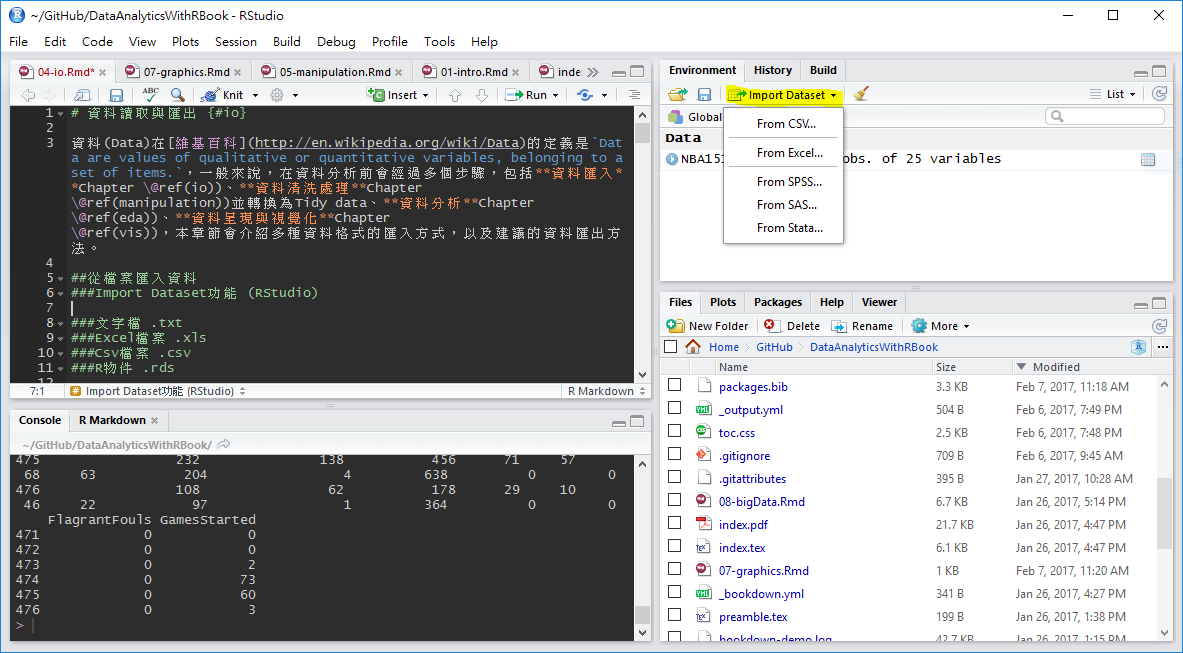
\includegraphics[width=16.43in]{figure/import}

以csv檔案為例,在選單中選取\texttt{From\ CSV},選取後會跳出資料匯入輔助視窗,點選\texttt{Browse}按鈕開啟檔案選取器,並點選欲匯入之文字檔案

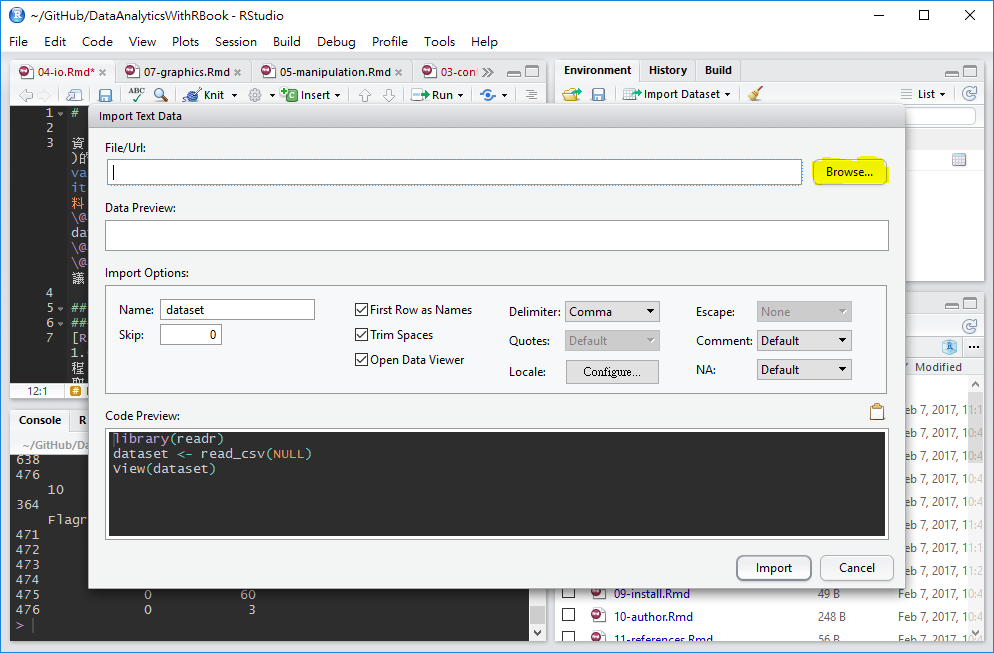
\includegraphics[width=13.81in]{figure/csv}

檔案選取後,資料匯入輔助視窗有預覽功能,供使用者檢查資料匯入方法是否正確,若需調整各項參數,可利用下方\texttt{Import\ Options}的選項微調,最常用的調整功能是\texttt{Delimiter}分隔符號與\texttt{First\ Row\ as\ Names}首列是否為欄位名稱。

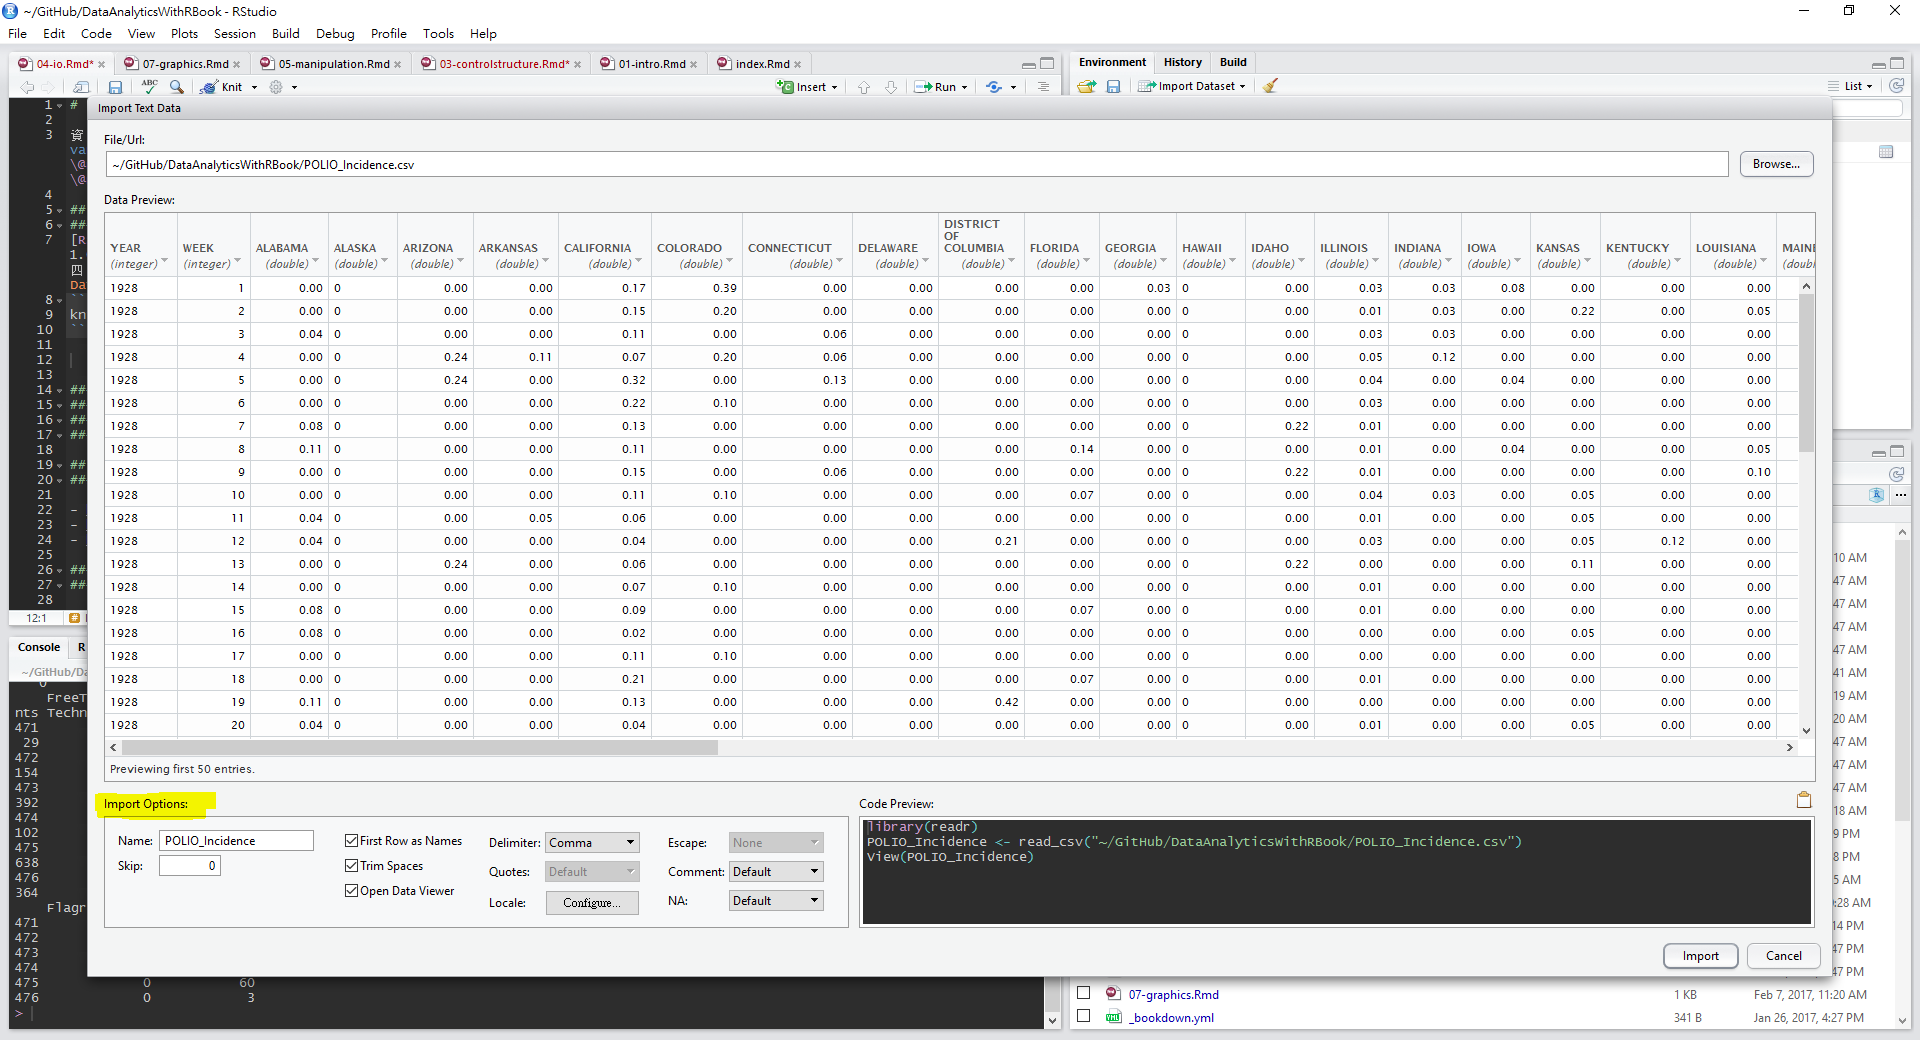
\includegraphics[width=26.67in]{figure/csv2}

如果要匯入的檔案為\textbf{tab分隔文字檔},一樣可以選擇\texttt{.csv}選項,再修改\texttt{Delimiter}參數為\texttt{Tab}即可。

資料匯入輔助視窗右下方\texttt{Code\ Preview:}子視窗中會自動產生資料匯入程式碼,如果未來想再使用視窗匯入,希望透過程式碼匯入,可以將此段程式碼複製貼上到R程式碼檔案(.R),供後續分析使用。

\subsection{分隔文字檔 .txt}\label{-.txt}

\texttt{readr} \citep{R-readr}
package提供完整的文字檔讀取功能,各讀取函數的第一個參數通常為\textbf{檔案路徑與名稱},\texttt{read\_delim()}函數可用來讀取所有用分隔符號分隔的文字檔案,以tab分隔為例,只需將\texttt{delim}參數設定為\texttt{\textbackslash{}t},即可用tab將各欄位分開讀取。此外,\texttt{col\_names}參數也常被使用,TRUE代表資料內有包含欄位名稱(通常在首列),預設為TRUE,如果設定為FALSE,欄位名稱則會依順序被設定為
X1, X2, X3 \ldots{}。

參數整理如下 (可用?read\_delim指令閱讀官方說明):

\begin{itemize}
\tightlist
\item
  \texttt{file}, 檔名
\item
  \texttt{delim}, 分隔符號
\item
  \texttt{quote}, 把欄位包起來的符號
\item
  \texttt{escape\_backslash}, 預設FALSE,是否用/作為逃脫符號
\item
  \texttt{escape\_double}, 預設TRUE,是否用quote符號作為逃脫符號
\item
  \texttt{col\_names}, 是否有欄位名稱(表頭)(T/F)
\item
  \texttt{col\_types}, 每一個欄位的類別,用向量表示
\item
  \texttt{comment}, 備註標示符號,在備註標示符號之後的文字不會被讀入
\item
  \texttt{skip}, 要跳過幾行?
\end{itemize}

\begin{Shaded}
\begin{Highlighting}[]
\KeywordTok{library}\NormalTok{(readr)}
\NormalTok{dataset <-}\StringTok{ }\KeywordTok{read_delim}\NormalTok{(}\StringTok{"檔案路徑與名稱"}\NormalTok{, }\DataTypeTok{delim=}\StringTok{"}\CharTok{\textbackslash{}t}\StringTok{"}\NormalTok{)}
\end{Highlighting}
\end{Shaded}

\subsection{CSV檔案 .csv}\label{csv}

\texttt{readr} \citep{R-readr} package也提供CSV
(逗號分隔)檔案的讀取功能,\texttt{read\_csv()}

\begin{Shaded}
\begin{Highlighting}[]
\KeywordTok{library}\NormalTok{(readr)}
\NormalTok{dataset <-}\StringTok{ }\KeywordTok{read_csv}\NormalTok{(}\StringTok{"檔案路徑與名稱"}\NormalTok{)}
\end{Highlighting}
\end{Shaded}

\subsection{Excel檔案 .xls}\label{excel-.xls}

\texttt{readxl} \citep{R-readxl} package提供讀取Excel檔案 (xls,
xlsx)的函數\texttt{read\_excel()},除了常用的\texttt{col\_names}參數外,也可使用\texttt{sheet}參數設定要讀取的工作表(sheet)

\begin{Shaded}
\begin{Highlighting}[]
\KeywordTok{library}\NormalTok{(readxl)}
\NormalTok{dataset <-}\StringTok{ }\KeywordTok{read_excel}\NormalTok{(}\StringTok{"檔案路徑與名稱"}\NormalTok{)}
\end{Highlighting}
\end{Shaded}

\subsection{R物件 .rds}\label{r-.rds}

R物件有檔案小與讀取快速的優點,如果在R程式處理資料後必須儲存一份以供後續分析的話,使用R物件儲存是最佳的方式,讀取R物件有多種函數可供選擇,推薦使用\texttt{readRDS()}函數
(參考資料:\href{http://www.fromthebottomoftheheap.net/2012/04/01/saving-and-loading-r-objects/}{A
better way of saving and loading objects in R})

\begin{Shaded}
\begin{Highlighting}[]
\NormalTok{dataset <-}\StringTok{ }\KeywordTok{readRDS}\NormalTok{(}\StringTok{"檔案路徑與名稱"}\NormalTok{)}
\end{Highlighting}
\end{Shaded}

\subsection{R程式 .R}\label{r-.r}

\texttt{source}, 讀R的Obejct or script, 執行, ASCII
(\texttt{dump}的相反)

\subsection{純文字資料 (無分隔)}\label{-}

\texttt{readLines}, 逐行讀取文字資料

\subsection{其他格式}

透過載入套件,R可讀入許多其他格式的檔案:

\begin{itemize}
\tightlist
\item
  MySQL \texttt{RMySQL}
\item
  HDF5 \texttt{rhdf5}
\item
  Weka \texttt{foreign}
\item
  Stata \texttt{foreign}
\item
  SPSS \texttt{Hmisc}
\item
  SAS \texttt{Hmisc}
\item
  GIS \texttt{rgdal}
\item
  Images \texttt{jpeg}
\item
  Music \texttt{tuneR}
\end{itemize}

\subsection{其他讀檔注意事項}

讀檔的時候R會自動

\begin{itemize}
\tightlist
\item
  跳過\#開頭的任何行(Row)
\item
  判斷要讀幾行
\item
  判斷每個列(Column)的類別
\item
  把欄位包起來的符號
\end{itemize}

如果讀取時已指定\textbf{Column類別}以及\textbf{把欄位包起來的符號},讀取速度會快很多。

\section{從網路匯入資料}

\subsection{Open Data}\label{open-data}

\textbf{開放資料} (Open data)
指的是一種經過挑選與許可的資料,這些資料不受著作權、專利權,以及其他管理機制所限制,可以開放給社會公眾,任何人都可以自由出版使用,不論是要拿來出版或是做其他的運用都不加以限制。Open
data
運動希望達成的目標與開放原始碼、內容開放、開放獲取等其他「開放」運動類似。Open
data 背後的核心思想由來已,但 Open data
這名詞直到近代才出現,拜網際網路崛起而為人所知,尤其是 Data.gov 等 Open
data
政府組織的設立。(\href{https://zh.wikipedia.org/wiki/\%E9\%96\%8B\%E6\%94\%BE\%E8\%B3\%87\%E6\%96\%99}{維基百科})

台灣政府從2011年開始大力推動開放政府與開放資料的概念,多個機關與縣市政府架設開放資料平台,供民眾擷取或再利用各項資料

\begin{itemize}
\tightlist
\item
  \href{http://data.gov.tw/}{政府資料開放平台}
\item
  \href{http://data.taipei/}{Data Taipei}
\item
  \href{http://data.tycg.gov.tw/}{開放資料 x 開放桃園}
\item
  \href{http://data.moi.gov.tw/}{內政資料開放平台}
\end{itemize}

Open Data常見的儲存方式為: \texttt{CSV}Chapter
\ref{csv}、\texttt{JSON}Chapter \ref{json}、\texttt{XML}Chapter
\ref{xml},開放資料網站通常有提供民眾\textbf{直接下載}檔案的服務,針對可下載的CSV格式資料,可以下載完成後,透過上述\textbf{由檔案匯入資料}
Chapter \ref{file}方法匯入即可。

\subsection{API (Application programming interfaces)}\label{api}

應用程式介面 Application programming interfaces (API)
通常是特定軟體、程序或系統,廠商或開發人員,為了能夠讓第三方的開發者可以額外開發應用程式來強化他們的產品,所推出可以與他們系統溝通的介面。(\href{https://zh.wikipedia.org/zh-tw/\%E5\%BA\%94\%E7\%94\%A8\%E7\%A8\%8B\%E5\%BA\%8F\%E6\%8E\%A5\%E5\%8F\%A3}{維基百科})

以下載Open
Data為例,若檔案更新頻繁,使用手動下載相當耗時。如\href{http://data.taipei/opendata/datalist/datasetMeta?oid=6a3e862a-e1cb-4e44-b989-d35609559463}{臺北市開放認養動物}資料,更新頻率為每日,所以許多開放資料也提供透過\textbf{API}下載的服務,透過API下載的資料格式會是JSON格式Chapter
\ref{json},如\href{http://data.taipei/opendata/datalist/datasetMeta/outboundDesc?id=6a3e862a-e1cb-4e44-b989-d35609559463\&rid=f4a75ba9-7721-4363-884d-c3820b0b917c}{臺北市開放認養動物API資訊}所示,開放資料網站會提供\textbf{資料集ID}與\textbf{資料RID}

\begin{itemize}
\tightlist
\item
  \textbf{資料集ID}: 紀錄資料的基本參數,如包含欄位、更新頻率等
\item
  \textbf{資料RID}: 資料集
\end{itemize}

並同時提供擷取範例,如果需要下載原始資料,可直接從範例複製貼上即可,如http://data.taipei/opendata/datalist/apiAccess?scope=resourceAquire\&rid=f4a75ba9-7721-4363-884d-c3820b0b917c

\subsection{JSON格式檔案}\label{json}

JSON (\textbf{J}ava\textbf{s}cript \textbf{O}bject
\textbf{N}otation)是一種輕量級的資料交換語言
(\href{http://en.wikipedia.org/wiki/JSON}{Wiki}),特色如下:

\begin{itemize}
\tightlist
\item
  from \textbf{a}pplication \textbf{p}rogramming \textbf{i}nterfaces
  (APIs)
\item
  JavaScript、Java、Node.js應用
\item
  一些NoSQL非關連型資料庫用JSON儲存資料:\textbf{MongoDB}
\item
  資料儲存格式

  \begin{itemize}
  \tightlist
  \item
    Numbers (double)
  \item
    Strings (double quoted)
  \item
    Boolean (\emph{true} or \emph{false})
  \item
    Array (ordered, comma separated enclosed in square brackets
    \emph{\protect\hyperlink{preface}{}})
  \item
    Object (unorderd, comma separated collection of \textbf{key:value}
    pairs in curley brackets \emph{\{\}})
  \end{itemize}
\end{itemize}

\href{https://api.github.com/users/yijutseng/repos}{JSON檔案範例}

許多Open
Data也用JSON格式儲存,例如\href{http://data.taipei/opendata/datalist/datasetMeta?oid=6a3e862a-e1cb-4e44-b989-d35609559463}{臺北市開放認養動物}資料,根據資料的API資訊,可得資料擷取網址http://data.taipei/opendata/datalist/apiAccess?scope=resourceAquire\&rid=f4a75ba9-7721-4363-884d-c3820b0b917c
。

將JSON檔案匯入R可以使用\texttt{jsonlite}\citep{R-jsonlite}
package,套件使用前必須安裝,安裝套件方法請參考Chapter
\ref{intro},載入後,可使用\texttt{fromJSON()}函數載入JSON資料。
如API網址為\textbf{httr}類別,需要載入\texttt{httr}\citep{Rhttr}
package,並使用\texttt{GET()}函數處理資料擷取網址。

\begin{Shaded}
\begin{Highlighting}[]
\KeywordTok{library}\NormalTok{(jsonlite)}
\NormalTok{PetData<-}\KeywordTok{fromJSON}\NormalTok{(}\StringTok{"http://data.taipei/opendata/datalist/apiAccess?scope=resourceAquire&rid=f4a75ba9-7721-4363-884d-c3820b0b917c"}\NormalTok{)}
\KeywordTok{str}\NormalTok{(PetData)}
\end{Highlighting}
\end{Shaded}

\begin{verbatim}
## List of 1
##  $ result:List of 5
##   ..$ offset : int 0
##   ..$ limit  : int 10000
##   ..$ count  : int 307
##   ..$ sort   : chr ""
##   ..$ results:'data.frame':  307 obs. of  20 variables:
##   .. ..$ _id            : chr [1:307] "1" "2" "3" "4" ...
##   .. ..$ Name           : chr [1:307] "" "" "花俏" "麥茶" ...
##   .. ..$ Sex            : chr [1:307] "雄" "雌" "雌" "雄" ...
##   .. ..$ Type           : chr [1:307] "貓" "犬" "貓" "貓" ...
##   .. ..$ Build          : chr [1:307] "中" "中" "中" "中" ...
##   .. ..$ Age            : chr [1:307] "成年" "老年" "成年" "成年" ...
##   .. ..$ Variety        : chr [1:307] "米克斯" "米克斯" "米克斯" "米克斯" ...
##   .. ..$ Reason         : chr [1:307] "動物救援" "動物救援" "動物救援" "動物管制" ...
##   .. ..$ AcceptNum      : chr [1:307] "106032203" "106031503" "106031204" "106031003" ...
##   .. ..$ ChipNum        : chr [1:307] "" "" "" "" ...
##   .. ..$ IsSterilization: chr [1:307] "未絕育" "未絕育" "未絕育" "未絕育" ...
##   .. ..$ HairType       : chr [1:307] "黃白" "黑" "三花" "黃白" ...
##   .. ..$ Note           : chr [1:307] "神經症狀" "虛弱、瘦、左側大範圍外傷、無法站立" "大家好~我的名字叫花俏,漂亮的我想要找個長期飯票,這個人會是你嗎?讓我們給彼此一個機會吧!!\n" "大家好,我叫麥茶,\n淡淡憂鬱的我有吸引你嗎?\n個性有點緊張、怕人,\n要花時間慢慢培養感情,等待我熟悉,\n你願意給我機會,讓我進"| __truncated__ ...
##   .. ..$ Resettlement   : chr [1:307] "臺北市動物之家 收容編號106032203" "臺北市動物之家 收容編號:106031503" "臺北市動物之家 收容編號106031204" "臺北市動物之家 收容編號106031003" ...
##   .. ..$ Phone          : chr [1:307] "02-87913063" "02-8791-3063" "02-87913062" "02-87913062" ...
##   .. ..$ Email          : chr [1:307] "tcapoa8@mail.taipei.gov.tw" "tcapoa8@mail.taipei.gov.tw" "tcapoa8@mail.taipei.gov.tw" "tcapoa8@mail.taipei.gov.tw" ...
##   .. ..$ ChildreAnlong  : chr [1:307] "" "" "" "" ...
##   .. ..$ AnimalAnlong   : chr [1:307] "" "" "" "" ...
##   .. ..$ Bodyweight     : chr [1:307] "" "" "" "" ...
##   .. ..$ ImageName      : chr [1:307] "http://163.29.39.183/uploads/images/medium/9fe8fb19-ed6f-41a2-b25c-719a80559085.jpg" "http://163.29.39.183/uploads/images/medium/6b77ae0f-e893-4bca-af97-c6e9afd36d2e.jpg" "http://163.29.39.183/uploads/images/medium/e0de6dfd-332e-459b-b157-36b006a1924c.jpg" "http://163.29.39.183/uploads/images/medium/c5983ea5-b55a-4bd1-bb3b-2c03f8e496a2.jpg" ...
\end{verbatim}

由資料結構可知,經過\texttt{fromJSON()}函數匯入的JSON檔案被轉存為\texttt{列表list}的型態,且在result元素中包含五個子元素(offset,
limit, count, sort,
results),其中,results子元素的類別為資料框data.frame,內含開放認養動物清單,因此,可使用\texttt{\$}符號截取元素與子元素

\begin{Shaded}
\begin{Highlighting}[]
\KeywordTok{head}\NormalTok{(PetData$result$results)}
\end{Highlighting}
\end{Shaded}

\begin{verbatim}
##   _id Name Sex Type Build  Age Variety   Reason AcceptNum ChipNum
## 1   1       雄   貓    中 成年  米克斯 動物救援 106032203        
## 2   2       雌   犬    中 老年  米克斯 動物救援 106031503        
## 3   3 花俏  雌   貓    中 成年  米克斯 動物救援 106031204        
## 4   4 麥茶  雄   貓    中 成年  米克斯 動物管制 106031003        
## 5   5 山姆  雄   貓    中 成年  米克斯 民眾拾獲 106031002        
## 6   6       雌   犬    幼 幼齡  米克斯 民眾拾獲 106031021        
##   IsSterilization HairType
## 1          未絕育     黃白
## 2          未絕育       黑
## 3          未絕育     三花
## 4          未絕育     黃白
## 5          未絕育   黃虎斑
## 6          未絕育       黑
##                                                                                                                                                                    Note
## 1                                                                                                                                                              神經症狀
## 2                                                                                                                                    虛弱、瘦、左側大範圍外傷、無法站立
## 3                                                                            大家好~我的名字叫花俏,漂亮的我想要找個長期飯票,這個人會是你嗎?讓我們給彼此一個機會吧!!\n
## 4 大家好,我叫麥茶,\n淡淡憂鬱的我有吸引你嗎?\n個性有點緊張、怕人,\n要花時間慢慢培養感情,等待我熟悉,\n你願意給我機會,讓我進入你的家庭嗎,\n歡迎來動物之家看看我唷!
## 5                                                                                          臉傷。\n嗨~我的名字叫山姆,我的個性比較緊張,請多給我一點時間適應新環境唷!\n
## 6                                                                                                                                                                      
##                         Resettlement        Phone                      Email
## 1   臺北市動物之家 收容編號106032203  02-87913063 tcapoa8@mail.taipei.gov.tw
## 2 臺北市動物之家 收容編號:106031503 02-8791-3063 tcapoa8@mail.taipei.gov.tw
## 3   臺北市動物之家 收容編號106031204  02-87913062 tcapoa8@mail.taipei.gov.tw
## 4   臺北市動物之家 收容編號106031003  02-87913062 tcapoa8@mail.taipei.gov.tw
## 5   臺北市動物之家 收容編號106031002  02-87913062 tcapoa8@mail.taipei.gov.tw
## 6   臺北市動物之家 收容編號106031021  02-87913062 tcapoa8@mail.taipei.gov.tw
##   ChildreAnlong AnimalAnlong Bodyweight
## 1                                      
## 2                                      
## 3                                      
## 4                                      
## 5                                      
## 6                                      
##                                                                             ImageName
## 1 http://163.29.39.183/uploads/images/medium/9fe8fb19-ed6f-41a2-b25c-719a80559085.jpg
## 2 http://163.29.39.183/uploads/images/medium/6b77ae0f-e893-4bca-af97-c6e9afd36d2e.jpg
## 3 http://163.29.39.183/uploads/images/medium/e0de6dfd-332e-459b-b157-36b006a1924c.jpg
## 4 http://163.29.39.183/uploads/images/medium/c5983ea5-b55a-4bd1-bb3b-2c03f8e496a2.jpg
## 5 http://163.29.39.183/uploads/images/medium/478ca5ce-4bc2-46c7-a22f-dd8c2bf7ed77.jpg
## 6 http://163.29.39.183/uploads/images/medium/c9318c07-988d-4ac4-b7ba-ddba0968759c.jpg
\end{verbatim}

results資料框中包含20個欄位,可以像分析資料框一樣,針對此資料框做分析,舉例來說,可分析各項\textbf{開放認養理由}出現次數

\begin{Shaded}
\begin{Highlighting}[]
\KeywordTok{table}\NormalTok{(PetData$result$results$Reason)}
\end{Highlighting}
\end{Shaded}

\begin{verbatim}
## 
##                  動物救援     動物管制 民眾不擬續養     民眾拾獲 
##           26           93          121           44           23
\end{verbatim}

分析可知開放認養理由以動物管制與未填寫居多。

如果需要將資料框轉換成JSON檔案可以使用\texttt{jsonlite}
package所提供的\texttt{toJSON()}函數。

\begin{Shaded}
\begin{Highlighting}[]
\NormalTok{myjson <-}\StringTok{ }\KeywordTok{toJSON}\NormalTok{(iris, }\DataTypeTok{pretty=}\OtherTok{TRUE}\NormalTok{)}
\KeywordTok{str}\NormalTok{(myjson)}
\end{Highlighting}
\end{Shaded}

\begin{verbatim}
## Class 'json'  chr "[\n  {\n    \"Sepal.Length\": 5.1,\n    \"Sepal.Width\": 3.5,\n    \"Petal.Length\": 1.4,\n    \"Petal.Width\": 0.2\n  },\n  {\"| __truncated__
\end{verbatim}

\subsection{XML 可延伸標記式語言}\label{xml}

\begin{itemize}
\tightlist
\item
  E\textbf{x}tensible \textbf{m}arkup \textbf{l}anguage
\item
  描述\textbf{結構化}資料的語言
\item
  處理XML檔案是網頁\textbf{Html}爬蟲的基礎
\item
  Components

  \begin{itemize}
  \tightlist
  \item
    Markup 標記 - labels that give the text structure
  \item
    Content 內文 - the actual text of the document
  \end{itemize}
\item
  \href{https://zh.wikipedia.org/wiki/XML}{XML Wiki}
\end{itemize}

Tags, elements and attributes

\begin{itemize}
\tightlist
\item
  Tags correspond to general labels

  \begin{itemize}
  \tightlist
  \item
    Start tags \texttt{\textless{}breakfast\_menu\textgreater{}},
    \texttt{\textless{}price\textgreater{}}
  \item
    End tags
    \texttt{\textless{}/breakfast\_menu\textgreater{}},\texttt{\textless{}/price\textgreater{}}
  \item
    Empty tags \texttt{\textless{}line-break\ /\textgreater{}}
  \end{itemize}
\item
  Elements are specific examples of tags

  \begin{itemize}
  \tightlist
  \item
    \texttt{\textless{}name\textgreater{}Belgian\ Waffles\textless{}/name\textgreater{}}
  \end{itemize}
\item
  Attributes are components of the label

  \begin{itemize}
  \tightlist
  \item
    \texttt{\textless{}book\ category="web"\textgreater{}}
  \end{itemize}
\end{itemize}

許多Open
Data也用XML格式儲存,例如\href{http://data.taipei/opendata/datalist/datasetMeta/download?id=961ca397-4a59-45e8-b312-697f26b059dc\&rid=190796c8-7c56-42e0-8068-39242b8ec927}{臺北市水質監測資訊}。如需將XML檔案匯入R中,需要安裝\texttt{XML}
\citep{R-XML} package,使用\texttt{xmlParse()}函數將檔案匯入。

\begin{Shaded}
\begin{Highlighting}[]
\KeywordTok{library}\NormalTok{(XML)}
\NormalTok{waterQ <-}\StringTok{ }\KeywordTok{xmlParse}\NormalTok{(}\StringTok{"http://data.taipei/opendata/datalist/datasetMeta/download?id=961ca397-4a59-45e8-b312-697f26b059dc&rid=190796c8-7c56-42e0-8068-39242b8ec927"}\NormalTok{)}
\end{Highlighting}
\end{Shaded}

完成資料讀取後,使用\texttt{xpathSApply()}函數搭配\textbf{XPath}語法取得指定標籤內的資料

\begin{Shaded}
\begin{Highlighting}[]
\CommentTok{#取得所有"code_name"標籤內的資料}
\KeywordTok{xpathSApply}\NormalTok{(waterQ,}\StringTok{"//code_name"}\NormalTok{,xmlValue)[}\DecValTok{1}\NormalTok{:}\DecValTok{10}\NormalTok{]}
\end{Highlighting}
\end{Shaded}

\begin{verbatim}
##  [1] "雙溪淨水場"               "衛理女中"                
##  [3] "雙溪國小                " "華興加壓站"              
##  [5] "長興淨水場"               "市政大樓"                
##  [7] "市議會"                   "捷運忠孝復興站"          
##  [9] "南港高工"                 "南港加壓站"
\end{verbatim}

\begin{Shaded}
\begin{Highlighting}[]
\CommentTok{#取得各監測站的經度}
\KeywordTok{xpathSApply}\NormalTok{(waterQ,}\StringTok{"//longitude"}\NormalTok{,xmlValue)[}\DecValTok{1}\NormalTok{:}\DecValTok{10}\NormalTok{]}
\end{Highlighting}
\end{Shaded}

\begin{verbatim}
##  [1] "121.56094" "121.54401" "121.55557" "121.53476" "121.54043" "121.55661"
##  [7] "121.55360" "121.53551" "121.59892" "121.60829"
\end{verbatim}

\textbf{XPath}是XML路徑語言(XML Path
Language),基於XML的樹狀結構,提供在資料結構樹中找尋節點的能力,\textbf{XPath}語法的邏輯,可參考\href{https://www.w3schools.com/xml/xpath_syntax.asp}{W3C
Schools}或是Google搜尋相關中文教學。在此列舉幾個常用的語法:

\begin{verbatim}
// : 子結點資料, 如所有連結標籤 //a
@ : 屬性資料, 如所有連結標籤內的連結網址 //a/@href
\end{verbatim}

\subsection{網頁爬蟲 Webscraping}\label{-webscraping}

由於不是每個網站都提供API,但網頁上卻有你想要分析的資料(像是ptt推文!?),除了人工複製貼上以外,也可以將網頁處理程式化,以程式化的方式擷取網頁資料就叫做\textbf{網頁爬蟲(Webscraping)}(\href{http://en.wikipedia.org/wiki/Web_scraping}{Webscraping
Wiki})。在R中可以直接把HTML檔案當作XML檔案處理分析,也可使用\texttt{rvest}\citep{R-rvest}
package輔助爬蟲程式撰寫。

此外,網頁爬蟲可能耗費很多網頁流量和資源,所以在許多網站被視為非法行為,如果一次讀太多太快,很可能被鎖IP。

以\href{http://im.cgu.edu.tw/bin/home.php}{長庚資管系}網站為例,可直接逐行讀取
\texttt{readLines()}

\begin{Shaded}
\begin{Highlighting}[]
\NormalTok{con <-}\StringTok{ }\KeywordTok{url}\NormalTok{(}\StringTok{"http://im.cgu.edu.tw/bin/home.php"}\NormalTok{)}
\NormalTok{htmlCode <-}\KeywordTok{readLines}\NormalTok{(con)}
\end{Highlighting}
\end{Shaded}

\begin{verbatim}
## Warning in readLines(con): incomplete final line found on 'http://im.cgu.edu.tw/
## bin/home.php'
\end{verbatim}

\begin{Shaded}
\begin{Highlighting}[]
\KeywordTok{close}\NormalTok{(con)}
\NormalTok{htmlCode[}\DecValTok{1}\NormalTok{:}\DecValTok{5}\NormalTok{]}
\end{Highlighting}
\end{Shaded}

\begin{verbatim}
## [1] "<!DOCTYPE html PUBLIC \"-//W3C//DTD XHTML 1.0 Transitional//EN\" \"http://www.w3.org/TR/xhtml1/DTD/xhtml1-transitional.dtd\">"                
## [2] "<html xmlns=\"http://www.w3.org/1999/xhtml\" lang=\"zh-tw\">"                                                                                 
## [3] "<head>"                                                                                                                                       
## [4] "<meta http-equiv=\"Content-Type\" content=\"text/html; charset=utf-8\" />"                                                                    
## [5] "<meta http-equiv=\"X-UA-Compatible\" content=\"IE=EmulateIE7\" /><meta name=\"keywords\" content=\"請填寫網站關鍵記事,用半角逗號(,)隔開\" />"
\end{verbatim}

或是使用XML工具分析擷取網頁 (\texttt{XML}
package),使用方法與XML檔案處理方法類似,搭配\textbf{XPath}語言,篩選所需資料

\begin{Shaded}
\begin{Highlighting}[]
\NormalTok{html <-}\StringTok{ }\KeywordTok{htmlParse}\NormalTok{(}\StringTok{"http://im.cgu.edu.tw/bin/home.php"}\NormalTok{)}
\KeywordTok{xpathSApply}\NormalTok{(html, }\StringTok{"//title"}\NormalTok{, xmlValue)}
\end{Highlighting}
\end{Shaded}

\begin{verbatim}
## [1] "長庚大學 資訊管理學系 "
\end{verbatim}

\begin{Shaded}
\begin{Highlighting}[]
\KeywordTok{xpathSApply}\NormalTok{(html, }\StringTok{"//span[@class='ptname ']"}\NormalTok{, xmlValue)}
\end{Highlighting}
\end{Shaded}

\begin{verbatim}
##  [1] "畢業專題成果展"       "碩士班計畫書審查"     "畢業校友資料登錄"    
##  [4] "長庚大學首頁"         "校務資訊系統"         "人事教育訓練資訊網"  
##  [7] "資管系導師名單"       "TA課後輔導值班表"     "碩博士論文網"        
## [10] "國內資管系所"         "資管系內部行政系統"   "資管系分機表"        
## [13] "資管系學會"           "工商管理學系/研究所"  "工業設計學系/研究所" 
## [16] "管理學院"             "醫務管理學系/研究所"  "商管專業學院"        
## [19] "企業管理研究所博士班" "長庚大學行事曆"
\end{verbatim}

除了把HTML檔案當作XML處理外,\texttt{rvest}\citep{R-rvest}
package是R語言中最常被使用的爬蟲套件,使用前一樣需要安裝與載入

\begin{Shaded}
\begin{Highlighting}[]
\KeywordTok{install.packages}\NormalTok{(}\StringTok{"rvest"}\NormalTok{) ##安裝}
\end{Highlighting}
\end{Shaded}

\begin{Shaded}
\begin{Highlighting}[]
\KeywordTok{library}\NormalTok{(rvest) ##載入}
\end{Highlighting}
\end{Shaded}

載入\texttt{rvest}套件後,經由以下步驟進行網站解析:

\begin{itemize}
\tightlist
\item
  使用\texttt{read\_html(“欲擷取的網站網址”)}函數讀取網頁
\item
  使用\texttt{html\_nodes()}函數擷取所需內容 (條件為CSS或xpath標籤)
\item
  使用\texttt{html\_text()}函數處理/清洗擷取內容,留下需要的資料
\item
  使用\texttt{html\_attr()}函數擷取資料參數(如連結url)
\end{itemize}

\begin{Shaded}
\begin{Highlighting}[]
\NormalTok{YahooNewsurl=}\StringTok{"https://tw.news.yahoo.com/"}
\NormalTok{news_title =}\StringTok{ }\KeywordTok{read_html}\NormalTok{(YahooNewsurl) %>%}\StringTok{ }\KeywordTok{html_nodes}\NormalTok{(}\StringTok{".tpl-title a"}\NormalTok{) %>%}\StringTok{ }\KeywordTok{html_text}\NormalTok{()}
\NormalTok{news_url =}\StringTok{ }\KeywordTok{read_html}\NormalTok{(YahooNewsurl) %>%}\StringTok{ }\KeywordTok{html_nodes}\NormalTok{(}\StringTok{".tpl-title a"}\NormalTok{) %>%}\StringTok{ }\KeywordTok{html_attr}\NormalTok{(}\StringTok{"href"}\NormalTok{)}
\NormalTok{Yahoo_news =}\StringTok{ }\KeywordTok{data.frame}\NormalTok{(}\DataTypeTok{title =} \NormalTok{news_title, }\DataTypeTok{url=}\NormalTok{news_url)}
\KeywordTok{head}\NormalTok{(Yahoo_news)}
\end{Highlighting}
\end{Shaded}

\begin{verbatim}
                                    title                                                           url
1         曾1妻5妾好風光 男星慘賣豪宅還債 /從1妻5妾的風光到變賣豪宅還債-網友噓雷洪:活該-091741737.html
2          美報告:美棄「一中」台灣更危險               /美報告-美拋棄-中-台灣處境更危險-081036215.html
3           藍色凍蕃薯!1張圖看寒流有多冷       /霸王級寒流再襲台-張圖看懂這波寒流有多強-101500692.html
4           他被妻子戴綠帽 對象竟是親弟弟                 /他被妻子戴綠帽-對象竟是親弟弟-072010033.html
5               匆忙推出移民禁令 他後悔了           /匆忙推移民禁令-美國土安全部長表後悔-044517088.html
6 蔡政府對釣魚台態度 國民黨憂美日安保質變       /蔡政府對釣魚台態度-國民黨憂美日安保質變-160200179.html
\end{verbatim}

在\texttt{html\_nodes()}、\texttt{html\_text()}和\texttt{html\_attr()}函數中,擷取條件的撰寫會因網頁語法不同而有差異,必須要使用\textbf{Google
Chrome開發工具}等工具輔助觀察需要擷取資料的條件。以上述Yahoo新聞為例,需要擷取的資料所在HTML片段如下:

\begin{verbatim}
<ul class="tpl-title yom-list list-style-none" id="yui_3_9_1_1_1486568229946_2408">
<li class="list-story first" id="yui_3_9_1_1_1486568229946_2407">
<div class="txt" id="yui_3_9_1_1_1486568229946_2406">
<a href="/從1妻5妾的風光到變賣豪宅還債-網友噓雷洪:活該-091741737.html" class="title " data-ylk="pkg:96a0ca11-47bc-3100-81ad-0a288707f150;ver:60cdb126-ee0c-11e6-bb9b-8a777738a932;lt:i;pos:1;" data-rapid_p="1">曾1妻5妾好風光 男星慘賣豪宅還債</a>
<cite id="yui_3_9_1_1_1486568229946_2405">
<span class="provider" id="yui_3_9_1_1_1486568229946_2404">Yahoo奇摩娛樂新聞</span>
</cite></div></li>
....
\end{verbatim}

觀察上述程式碼可已發現新聞清單被包含在\texttt{ul}標籤下,且css
class為\texttt{tpl-title\ yom-list\ list-style-none},所以這邊可以使用第一個class\texttt{tpl-title}為篩選條件。CSS
標籤的意義可參考\href{https://www.w3schools.com/cssref/css_selectors.asp}{W3C
Schools}的教學\{target=``\_blank``\}。

網頁爬蟲需要多做觀察與練習,才可熟知篩選技巧。

其他爬蟲相關參考資源:

\begin{itemize}
\tightlist
\item
  \href{https://www.slideshare.net/secret/mdfHLPgvIW1kPR}{網路爬蟲實作 -
  用 r 語言打造自己的爬蟲程式}
\item
  \href{https://github.com/hadley/rvest}{rvest GitHub}
\item
  R Bloggers
  有很多\href{http://www.r-bloggers.com/?s=Web+Scraping}{爬蟲範例}(英文)
\item
  \href{http://bryannotes.blogspot.tw/2014/08/r-ptt-wantedsocial-network-analysis.html}{Ptt爬蟲實作}
\item
  \href{http://www.largitdata.com/course_list/1}{大數學堂 網頁爬蟲課程}
\end{itemize}

\section{Facebook資料擷取}\label{facebook}

Facebook提供\href{https://developers.facebook.com/docs/graph-api?locale=zh_TW}{Graph
API},讓應用程式可透過API讀取與寫入 Facebook相關資料,\textbf{Graph
API}會根據篩選條件,回傳JSON格式的資料。除此之外,Facebook還提供\href{https://developers.facebook.com/tools/explorer/}{Graph
API Explorer},讓程式開發人員可以測試資料撈取方法和結果。
在開始使用\textbf{Graph API}之前,必須要取得自己的\textbf{access token}
(存取權杖),\href{https://developers.facebook.com/tools/explorer/}{Graph
API Explorer}工具提供\textbf{Get
Token}按鈕(通常在視窗右上角),可以讓開發者在不用新增應用程式(Application)的情況下取得暫時的\textbf{access
token}。

有關Facebook access
token的詳細介紹,可參考\href{https://developers.facebook.com/docs/facebook-login/access-tokens/?locale=zh_TW}{官方文件}

\subsection{Graph API in R}\label{graph-api-in-r}

\begin{Shaded}
\begin{Highlighting}[]
\KeywordTok{library}\NormalTok{(httr)}
\NormalTok{token<-}\StringTok{"your token"} \CommentTok{#將access token複製到此處 }
\NormalTok{FBData =}\StringTok{ }\KeywordTok{GET}\NormalTok{(}
    \KeywordTok{paste0}\NormalTok{(}\StringTok{"https://graph.facebook.com/v2.8/tsaiingwen?fields=posts%7Bmessage%7D&access_token="}\NormalTok{,}
           \NormalTok{token))}
\KeywordTok{names}\NormalTok{(FBData)}
\end{Highlighting}
\end{Shaded}

\begin{verbatim}
## [1] "url"         "status_code" "headers"     "all_headers" "cookies"     "content"     "date"       
## [8] "times"       "request"     "handle"    
\end{verbatim}

\begin{Shaded}
\begin{Highlighting}[]
\NormalTok{json1 =}\StringTok{ }\KeywordTok{content}\NormalTok{(FBData)}
\KeywordTok{names}\NormalTok{(json1)}
\end{Highlighting}
\end{Shaded}

\begin{verbatim}
## [1] "posts" "id"
\end{verbatim}

\begin{Shaded}
\begin{Highlighting}[]
\KeywordTok{names}\NormalTok{(json1$posts)}
\end{Highlighting}
\end{Shaded}

\begin{verbatim}
## [1] "data"   "paging"
\end{verbatim}

\begin{Shaded}
\begin{Highlighting}[]
\KeywordTok{head}\NormalTok{(json1$posts$data,}\DecValTok{3}\NormalTok{)}
\end{Highlighting}
\end{Shaded}

\begin{verbatim}
[[1]]
[[1]]$message
[1] "「國機國造」不是夢想,而是一個行動。今天啟動的高級教練機「自研自製」任務,是國防自主的重要里程碑。我們不只要讓戰機起飛,更要讓產業起飛。\n\n國防產業同樣是「5+2」關鍵產業之一,所以,除了要如期、如質完成新式高教機的「自研自製」外,也要重新厚植台灣的航太工業人才鏈,以及加強相關產業的連結、轉型和升級。\n\n國防自主沒有捷徑,只有努力再努力、堅持再堅持。今天,我們重新跨出歷史性的一步。"

[[1]]$id
[1] "46251501064_10154006497451065"


[[2]]
[[2]]$message
[1] "今天,智慧機械推動辦公室正式啟動。「落實產學合作」、「支持創新研發」、「強化行銷通路」是辦公室的三項重點任務。\n\n智慧機械是「5+2」關鍵產業的其中之一。政府有決心。我相信,所有的機械業者-無論做的是螺桿、刀庫、控制器或是工作母機,大家也都有很強的決心,要走向創新、走向智慧化、走向品牌。我們是一個團隊,我們一起加油!"

[[2]]$id
[1] "46251501064_10154006456601065"


[[3]]
[[3]]$message
[1] "今天來向台商拜個晚年。我也邀請台商朋友們,共同參與台灣經濟轉型升級的世紀工程。\n\n無論是擴大對國內的投資,或者配合新南向政策,前進海外深耕佈局,我期待跟台商朋友們一起努力,群策群力,克服困難和瓶頸,為台灣經濟發展打開全新的局面。"

[[3]]$id
[1] "46251501064_10154001652641065"
\end{verbatim}

\begin{Shaded}
\begin{Highlighting}[]
\NormalTok{json1$posts$data[[}\DecValTok{1}\NormalTok{]]$message}
\end{Highlighting}
\end{Shaded}

\begin{verbatim}
##[1] "「國機國造」不是夢想,而是一個行動。今天啟動的高級教練機「自研自製」任務,是國防自主的重要里程碑。我們不只要讓戰機起飛,更要讓產業起飛。\n\n國防產業同樣是「5+2」關鍵產業之一,所以,除了要如期、如質完成新式高教機的「自研自製」外,也要重新厚植台灣的航太工業人才鏈,以及加強相關產業的連結、轉型和升級。\n\n國防自主沒有捷徑,只有努力再努力、堅持再堅持。今天,我們重新跨出歷史性的一步。"
\end{verbatim}

\subsection{Rfacebook package}\label{rfacebook-package}

除了直接使用Graph API外,也可使用\texttt{Rfacebook}\citep{R-Rfacebook}
package來讀取Facebook資料。 以下為使用Rfacebook取得 \texttt{tsaiingwen}
粉絲頁的資料範例:

\begin{Shaded}
\begin{Highlighting}[]
\KeywordTok{library}\NormalTok{(Rfacebook)}
\NormalTok{token<-}\StringTok{"your token"} \CommentTok{#將token複製到此處 }
\KeywordTok{getPage}\NormalTok{(}\StringTok{"tsaiingwen"}\NormalTok{, token,}\DataTypeTok{n =} \DecValTok{5}\NormalTok{)}
\end{Highlighting}
\end{Shaded}

\begin{verbatim}
5 posts       from_id           from_name
1 46251501064 蔡英文 Tsai Ing-wen
2 46251501064 蔡英文 Tsai Ing-wen
3 46251501064 蔡英文 Tsai Ing-wen
4 46251501064 蔡英文 Tsai Ing-wen
5 46251501064 蔡英文 Tsai Ing-wen
                                                                                                                                                                                                                                                                                                                                                                                        message
1 「國機國造」不是夢想,而是一個行動。今天啟動的高級教練機「自研自製」任務,是國防自主的重要里程碑。我們不只要讓戰機起飛,更要讓產業起飛。\n\n國防產業同樣是「5+2」關鍵產業之一,所以,除了要如期、如質完成新式高教機的「自研自製」外,也要重新厚植台灣的航太工業人才鏈,以及加強相關產業的連結、轉型和升級。\n\n國防自主沒有捷徑,只有努力再努力、堅持再堅持。今天,我們重新跨出歷史性的一步。
2                                                                   今天,智慧機械推動辦公室正式啟動。「落實產學合作」、「支持創新研發」、「強化行銷通路」是辦公室的三項重點任務。\n\n智慧機械是「5+2」關鍵產業的其中之一。政府有決心。我相信,所有的機械業者-無論做的是螺桿、刀庫、控制器或是工作母機,大家也都有很強的決心,要走向創新、走向智慧化、走向品牌。我們是一個團隊,我們一起加油!
3                                                                                                                                                          今天來向台商拜個晚年。我也邀請台商朋友們,共同參與台灣經濟轉型升級的世紀工程。\n\n無論是擴大對國內的投資,或者配合新南向政策,前進海外深耕佈局,我期待跟台商朋友們一起努力,群策群力,克服困難和瓶頸,為台灣經濟發展打開全新的局面。
4                                                                                                                                                                                                                                                                                    「快了」!雞年通機捷,等待很值得。大年初四,我來看看機場捷運通車前的準備,也坐捷運到中壢,跟鄉親拜年問好。
5                                                                                                                                                                                                                                                                                                            雞年初三發福袋\n\n臺中豐原慈濟宮、彰化溪湖福安宮、雲林北港朝天宮、嘉義九華山地藏庵
              created_time  type
1 2017-02-07T08:02:45+0000 photo
2 2017-02-07T07:18:00+0000 photo
3 2017-02-05T07:12:52+0000 photo
4 2017-01-31T08:37:42+0000 photo
5 2017-01-30T11:41:07+0000 photo
                                                                                                    link
1 https://www.facebook.com/tsaiingwen/photos/a.390960786064.163647.46251501064/10154006497206065/?type=3
2 https://www.facebook.com/tsaiingwen/photos/a.390960786064.163647.46251501064/10154006455396065/?type=3
3 https://www.facebook.com/tsaiingwen/photos/a.390960786064.163647.46251501064/10154001652641065/?type=3
4 https://www.facebook.com/tsaiingwen/photos/a.390960786064.163647.46251501064/10153989357181065/?type=3
5 https://www.facebook.com/tsaiingwen/photos/a.390960786064.163647.46251501064/10153987089121065/?type=3
                             id likes_count comments_count shares_count
1 46251501064_10154006497451065        2013            125           43
2 46251501064_10154006456601065        2217            163           57
3 46251501064_10154001652641065        9416            920          163
4 46251501064_10153989358051065       34116           1574          373
5 46251501064_10153987095776065       20592            665          269
\end{verbatim}

由於每次擷取資料的比數有上限(大概是30筆左右),如果需要取得更多更長期的資料,就要使用迴圈協助,分批取得資料,透過設定
\textbf{since} 和 \textbf{until}參數,可設定資料擷取區間。

首先先取得日期向量,供後續迴圈做使用

\begin{Shaded}
\begin{Highlighting}[]
\NormalTok{lastDate<-}\KeywordTok{Sys.Date}\NormalTok{()}
\NormalTok{DateVector<-}\KeywordTok{seq}\NormalTok{(}\KeywordTok{as.Date}\NormalTok{(}\StringTok{"2017-01-01"}\NormalTok{),lastDate,}\DataTypeTok{by=}\StringTok{"5 days"}\NormalTok{)}
\NormalTok{DateVectorStr<-}\KeywordTok{as.character}\NormalTok{(DateVector)}
\NormalTok{DateVectorStr}
\end{Highlighting}
\end{Shaded}

\begin{verbatim}
## "2017-01-01" "2017-01-06" "2017-01-11" "2017-01-16" "2017-01-21" "2017-01-26" "2017-01-31" "2017-02-05"
\end{verbatim}

利用上述日期向量資料,搭配迴圈,依序設定\textbf{since} 和
\textbf{until}參數

\begin{Shaded}
\begin{Highlighting}[]
\NormalTok{totalPage<-}\OtherTok{NULL}
\NormalTok{token<-}\StringTok{'your token'}
\NormalTok{numberOfPost<-}\DecValTok{30}
\NormalTok{for(i in }\DecValTok{1}\NormalTok{:(}\KeywordTok{length}\NormalTok{(DateVectorStr)-}\DecValTok{1}\NormalTok{))\{}
    \NormalTok{tempPage<-}\KeywordTok{getPage}\NormalTok{(}\StringTok{"tsaiingwen"}\NormalTok{, token,}
                      \DataTypeTok{since =} \NormalTok{DateVectorStr[i],}\DataTypeTok{until =} \NormalTok{DateVectorStr[i}\DecValTok{+1}\NormalTok{])}
    \NormalTok{totalPage<-}\KeywordTok{rbind}\NormalTok{(totalPage,tempPage)}
\NormalTok{\}}
\KeywordTok{nrow}\NormalTok{(totalPage)}
\end{Highlighting}
\end{Shaded}

\begin{verbatim}
## 4 posts 8 posts 10 posts 3 posts 2 posts 14 posts 1 posts
## [1] 42
\end{verbatim}

Rfacebook Packages提供其他函數可供使用

\begin{itemize}
\tightlist
\item
  getUsers()
\item
  getPost()
\item
  searchFacebook()
\item
  Check \url{https://github.com/pablobarbera/Rfacebook}
\item
  ?Rfacebook
\end{itemize}

\section{資料匯出}

在R中完成資料處理後,有多種匯出選擇,如果是要匯出供他人在其他環境(如Excel)使用,建議匯出成tab分隔的文字檔(.txt)或是逗號分隔的文字檔(.csv);但若是要在R的環境繼續使用,建議匯出成R物件
(.rds),除了可保留欄位型別設定外,讀取速度與檔案大小皆優於文字檔案。

\subsection{文字檔 .txt}\label{-.txt}

使用\texttt{write.table()}函數寫入檔案,需要參數有

\begin{itemize}
\tightlist
\item
  \texttt{x} 要匯出的檔案,通常為matrix或是data.frame格式
\item
  \texttt{file} 檔案名稱
\item
  \texttt{append} T/F TRUE表示在檔案後端加入文字,F表示直接覆蓋原始檔案
  (預設F)
\item
  \texttt{quote} 是否需要用雙引號將字串包起 (預設T)
\item
  \texttt{sep} 分隔符號 (預設空白)
\item
  \texttt{eol} 換行符號
\item
  \texttt{na} 表示空值的字串
\item
  \texttt{dec} 小數點表示法
\item
  \texttt{row.names} T/F 是否需要輸出row names
\item
  \texttt{col.names} T/F 是否需要輸出column names
\item
  \texttt{qmethod} 逃脫字串設定
\item
  \texttt{fileEncoding} 編碼設定
\end{itemize}

\begin{Shaded}
\begin{Highlighting}[]
\KeywordTok{write.table}\NormalTok{(iris,}\DataTypeTok{file=}\StringTok{"iris.txt"}\NormalTok{,}\DataTypeTok{sep=}\StringTok{","}\NormalTok{,}\DataTypeTok{row.names =} \NormalTok{F,}\DataTypeTok{col.names =} \NormalTok{T)}
\end{Highlighting}
\end{Shaded}

\subsection{CSV檔 .csv}\label{csv-.csv}

與\texttt{write.table()}類似,使用\texttt{write.csv()}函數寫入檔案

\begin{Shaded}
\begin{Highlighting}[]
\KeywordTok{write.csv}\NormalTok{(iris,}\DataTypeTok{file=}\StringTok{"iris.csv"}\NormalTok{,}\DataTypeTok{row.names =} \NormalTok{F)}
\end{Highlighting}
\end{Shaded}

\subsection{R物件 .rds}\label{r-.rds-1}

若是要在R的環境繼續使用,建議匯出成R物件檔案(.rds)

\begin{Shaded}
\begin{Highlighting}[]
\KeywordTok{saveRDS}\NormalTok{(iris,}\StringTok{"iris.rds"}\NormalTok{)}
\end{Highlighting}
\end{Shaded}

\chapter{資料處理與清洗}\label{manipulation}

\section{Tidy Data}\label{tidy-data}

Each column is a variable. Each row is an observation.

\begin{itemize}
\tightlist
\item
  一個欄位(Column)內只有一個數值,最好要有凡人看得懂的Column Name
\item
  不同的觀察值應該要在不同行(Raw)
\item
  一張表裡面,有所有分析需要的資料
\item
  如果一定要多張表,中間一定要有index可以把表串起來
\item
  One file, one table
\end{itemize}

\section{資料型別轉換處理}

在資料型態章節Chapter \ref{DataType}中,曾介紹\textbf{數值
(numeric)}、\textbf{字串 (character)}、\textbf{布林變數
(logic)}以及\textbf{日期
(Date)}等資料型態,在此章節中將介紹如何檢查變數型別與各型別的轉換。

\subsection{資料型別檢查}

使用以下\texttt{is.}函數檢查資料型別,回傳布林變數,若為真,回傳TRUE

\begin{itemize}
\tightlist
\item
  是否為\textbf{數字} \texttt{is.numeric(變數名稱)}
\item
  是否為\textbf{文字} \texttt{is.character(變數名稱)}
\item
  是否為\textbf{布林變數} \texttt{is.logical(變數名稱)}
\end{itemize}

\begin{Shaded}
\begin{Highlighting}[]
\NormalTok{num<-}\DecValTok{100}
\NormalTok{cha<-}\StringTok{'200'}
\NormalTok{boo<-T}
\KeywordTok{is.numeric}\NormalTok{(num)}
\end{Highlighting}
\end{Shaded}

\begin{verbatim}
## [1] TRUE
\end{verbatim}

\begin{Shaded}
\begin{Highlighting}[]
\KeywordTok{is.numeric}\NormalTok{(cha)}
\end{Highlighting}
\end{Shaded}

\begin{verbatim}
## [1] FALSE
\end{verbatim}

\begin{Shaded}
\begin{Highlighting}[]
\KeywordTok{is.character}\NormalTok{(num)}
\end{Highlighting}
\end{Shaded}

\begin{verbatim}
## [1] FALSE
\end{verbatim}

\begin{Shaded}
\begin{Highlighting}[]
\KeywordTok{is.character}\NormalTok{(cha)}
\end{Highlighting}
\end{Shaded}

\begin{verbatim}
## [1] TRUE
\end{verbatim}

\begin{Shaded}
\begin{Highlighting}[]
\KeywordTok{is.logical}\NormalTok{(boo)}
\end{Highlighting}
\end{Shaded}

\begin{verbatim}
## [1] TRUE
\end{verbatim}

或使用\texttt{class(變數名稱)}函數,直接回傳資料型別

\begin{Shaded}
\begin{Highlighting}[]
\KeywordTok{class}\NormalTok{(num)}
\end{Highlighting}
\end{Shaded}

\begin{verbatim}
## [1] "numeric"
\end{verbatim}

\begin{Shaded}
\begin{Highlighting}[]
\KeywordTok{class}\NormalTok{(cha)}
\end{Highlighting}
\end{Shaded}

\begin{verbatim}
## [1] "character"
\end{verbatim}

\begin{Shaded}
\begin{Highlighting}[]
\KeywordTok{class}\NormalTok{(boo)}
\end{Highlighting}
\end{Shaded}

\begin{verbatim}
## [1] "logical"
\end{verbatim}

\begin{Shaded}
\begin{Highlighting}[]
\KeywordTok{class}\NormalTok{(}\KeywordTok{Sys.Date}\NormalTok{())}
\end{Highlighting}
\end{Shaded}

\begin{verbatim}
## [1] "Date"
\end{verbatim}

\subsection{資料型別轉換}

使用以下\texttt{as.}函數轉換型別

\begin{itemize}
\tightlist
\item
  轉換為\textbf{數字} \texttt{as.numeric(變數名稱)}
\item
  轉換為\textbf{文字} \texttt{as.character(變數名稱)}
\item
  轉換為\textbf{布林變數} \texttt{as.logical(變數名稱)}
\end{itemize}

\begin{Shaded}
\begin{Highlighting}[]
\KeywordTok{as.numeric}\NormalTok{(cha)}
\end{Highlighting}
\end{Shaded}

\begin{verbatim}
## [1] 200
\end{verbatim}

\begin{Shaded}
\begin{Highlighting}[]
\KeywordTok{as.numeric}\NormalTok{(boo)}
\end{Highlighting}
\end{Shaded}

\begin{verbatim}
## [1] 1
\end{verbatim}

\begin{Shaded}
\begin{Highlighting}[]
\KeywordTok{as.character}\NormalTok{(num)}
\end{Highlighting}
\end{Shaded}

\begin{verbatim}
## [1] "100"
\end{verbatim}

\begin{Shaded}
\begin{Highlighting}[]
\KeywordTok{as.character}\NormalTok{(boo)}
\end{Highlighting}
\end{Shaded}

\begin{verbatim}
## [1] "TRUE"
\end{verbatim}

若無法順利完成轉換,會回傳空值\texttt{NA},並出現警告訊息\texttt{Warning:\ NAs\ introduced\ by\ coercion,Warning:\ 強制變更過程中產生了\ NA}

\begin{Shaded}
\begin{Highlighting}[]
\KeywordTok{as.numeric}\NormalTok{(}\StringTok{"abc"}\NormalTok{)}
\end{Highlighting}
\end{Shaded}

\begin{verbatim}
## Warning: NAs introduced by coercion
\end{verbatim}

\begin{verbatim}
## [1] NA
\end{verbatim}

日期的轉換則建議使用\texttt{lubridate}\citep{R-lubridate}
package,如果想要將\texttt{年/月/日}格式的文字轉換為日期物件,可使用\texttt{ymd()}函數(y表年year,m表月month,d表日day),如果想要將\texttt{月/日/年}格式的文字轉換為日期物件,則使用\texttt{mdy()}函數,以此類推。

\begin{Shaded}
\begin{Highlighting}[]
\KeywordTok{library}\NormalTok{(lubridate)}
\KeywordTok{ymd}\NormalTok{(}\StringTok{'2012/3/3'}\NormalTok{)}
\end{Highlighting}
\end{Shaded}

\begin{verbatim}
## [1] "2012-03-03"
\end{verbatim}

\begin{Shaded}
\begin{Highlighting}[]
\KeywordTok{mdy}\NormalTok{(}\StringTok{'3/3/2012'}\NormalTok{)}
\end{Highlighting}
\end{Shaded}

\begin{verbatim}
## [1] "2012-03-03"
\end{verbatim}

\section{文字字串處理}

\subsection{基本處理}

\begin{itemize}
\tightlist
\item
  切割 \texttt{strsplit()}
\item
  子集 \texttt{substr()}
\item
  大小寫轉換 \texttt{toupper()} \texttt{tolower()}
\item
  兩文字連接 \texttt{paste()} \texttt{paste0()}
\item
  文字取代 \texttt{gsub()}
\item
  前後空白去除 \texttt{str\_trim()}
  需安裝\texttt{stringr}\citep{R-stringr} package
\end{itemize}

\begin{Shaded}
\begin{Highlighting}[]
\KeywordTok{strsplit} \NormalTok{(}\StringTok{"Hello World"}\NormalTok{,}\StringTok{" "}\NormalTok{)}
\end{Highlighting}
\end{Shaded}

\begin{verbatim}
## [[1]]
## [1] "Hello" "World"
\end{verbatim}

\begin{Shaded}
\begin{Highlighting}[]
\KeywordTok{toupper}\NormalTok{(}\StringTok{"Hello World"}\NormalTok{)}
\end{Highlighting}
\end{Shaded}

\begin{verbatim}
## [1] "HELLO WORLD"
\end{verbatim}

\begin{Shaded}
\begin{Highlighting}[]
\KeywordTok{tolower}\NormalTok{(}\StringTok{"Hello World"}\NormalTok{)}
\end{Highlighting}
\end{Shaded}

\begin{verbatim}
## [1] "hello world"
\end{verbatim}

\begin{Shaded}
\begin{Highlighting}[]
\KeywordTok{paste}\NormalTok{(}\StringTok{"Hello"}\NormalTok{, }\StringTok{"World"}\NormalTok{, }\DataTypeTok{sep=}\StringTok{''}\NormalTok{)}
\end{Highlighting}
\end{Shaded}

\begin{verbatim}
## [1] "HelloWorld"
\end{verbatim}

\begin{Shaded}
\begin{Highlighting}[]
\KeywordTok{substr}\NormalTok{(}\StringTok{"Hello World"}\NormalTok{, }\DataTypeTok{start=}\DecValTok{2}\NormalTok{,}\DataTypeTok{stop=}\DecValTok{4}\NormalTok{)}
\end{Highlighting}
\end{Shaded}

\begin{verbatim}
## [1] "ell"
\end{verbatim}

\begin{Shaded}
\begin{Highlighting}[]
\KeywordTok{gsub}\NormalTok{(}\StringTok{"o"}\NormalTok{,}\StringTok{"0"}\NormalTok{,}\StringTok{"Hello World"}\NormalTok{)}
\end{Highlighting}
\end{Shaded}

\begin{verbatim}
## [1] "Hell0 W0rld"
\end{verbatim}

\begin{Shaded}
\begin{Highlighting}[]
\KeywordTok{library}\NormalTok{(stringr)}
\KeywordTok{str_trim}\NormalTok{(}\StringTok{" Hello World "}\NormalTok{)}
\end{Highlighting}
\end{Shaded}

\begin{verbatim}
## [1] "Hello World"
\end{verbatim}

\subsection{搜尋字串}

搜尋字串函數通常使用在\textbf{比對文字向量},文字比對\textbf{有分大小寫},依照回傳值的型態不同,有兩種常用函數,\texttt{grep()}與\texttt{grepl()}:

\begin{itemize}
\tightlist
\item
  回傳符合條件之向量位置(index) \texttt{grep(搜尋條件,要搜尋的向量)}
\item
  回傳每個向量是否符合條件(TRUE or FALSE)
  \texttt{grepl(搜尋條件,要搜尋的向量)}
\end{itemize}

\begin{Shaded}
\begin{Highlighting}[]
\KeywordTok{grep}\NormalTok{(}\StringTok{"A"}\NormalTok{,}\KeywordTok{c}\NormalTok{(}\StringTok{"Alex"}\NormalTok{,}\StringTok{"Tom"}\NormalTok{,}\StringTok{"Amy"}\NormalTok{,}\StringTok{"Joy"}\NormalTok{,}\StringTok{"Emma"}\NormalTok{)) ##在姓名文字向量中尋找A,回傳包含"A"之元素位置}
\end{Highlighting}
\end{Shaded}

\begin{verbatim}
## [1] 1 3
\end{verbatim}

\begin{Shaded}
\begin{Highlighting}[]
\KeywordTok{grepl}\NormalTok{(}\StringTok{"A"}\NormalTok{,}\KeywordTok{c}\NormalTok{(}\StringTok{"Alex"}\NormalTok{,}\StringTok{"Tom"}\NormalTok{,}\StringTok{"Amy"}\NormalTok{,}\StringTok{"Joy"}\NormalTok{,}\StringTok{"Emma"}\NormalTok{)) ##在姓名文字向量中尋找A,回傳各元素是否包含"A"}
\end{Highlighting}
\end{Shaded}

\begin{verbatim}
## [1]  TRUE FALSE  TRUE FALSE FALSE
\end{verbatim}

\begin{Shaded}
\begin{Highlighting}[]
\KeywordTok{grepl}\NormalTok{(}\StringTok{"a"}\NormalTok{,}\KeywordTok{c}\NormalTok{(}\StringTok{"Alex"}\NormalTok{,}\StringTok{"Tom"}\NormalTok{,}\StringTok{"Amy"}\NormalTok{,}\StringTok{"Joy"}\NormalTok{,}\StringTok{"Emma"}\NormalTok{)) ##在姓名文字向量中尋找a,回傳各元素是否包含"a"}
\end{Highlighting}
\end{Shaded}

\begin{verbatim}
## [1] FALSE FALSE FALSE FALSE  TRUE
\end{verbatim}

\section{子集Subset}\label{subset}

\subsection{一維資料 (向量)}\label{-}

在向量章節\texttt{\{\#vector\}}有介紹使用\texttt{{[}{]}}取出單一或多個元素的方法

\begin{Shaded}
\begin{Highlighting}[]
\NormalTok{letters ##R語言內建資料之一}
\end{Highlighting}
\end{Shaded}

\begin{verbatim}
##  [1] "a" "b" "c" "d" "e" "f" "g" "h" "i" "j" "k" "l" "m" "n" "o" "p" "q" "r" "s"
## [20] "t" "u" "v" "w" "x" "y" "z"
\end{verbatim}

\begin{Shaded}
\begin{Highlighting}[]
\NormalTok{letters[}\DecValTok{1}\NormalTok{] ##取出letters向量的第一個元素}
\end{Highlighting}
\end{Shaded}

\begin{verbatim}
## [1] "a"
\end{verbatim}

\begin{Shaded}
\begin{Highlighting}[]
\NormalTok{letters[}\DecValTok{1}\NormalTok{:}\DecValTok{10}\NormalTok{] ##取出letters向量的前十個元素}
\end{Highlighting}
\end{Shaded}

\begin{verbatim}
##  [1] "a" "b" "c" "d" "e" "f" "g" "h" "i" "j"
\end{verbatim}

\begin{Shaded}
\begin{Highlighting}[]
\NormalTok{letters[}\KeywordTok{c}\NormalTok{(}\DecValTok{1}\NormalTok{,}\DecValTok{3}\NormalTok{,}\DecValTok{5}\NormalTok{)] ##取出letters向量的第1,3,5個元素}
\end{Highlighting}
\end{Shaded}

\begin{verbatim}
## [1] "a" "c" "e"
\end{verbatim}

\begin{Shaded}
\begin{Highlighting}[]
\NormalTok{letters[}\KeywordTok{c}\NormalTok{(-}\DecValTok{1}\NormalTok{,-}\DecValTok{3}\NormalTok{,-}\DecValTok{5}\NormalTok{)] ##取出letters向量除了第1,3,5個元素之外的所有元素}
\end{Highlighting}
\end{Shaded}

\begin{verbatim}
##  [1] "b" "d" "f" "g" "h" "i" "j" "k" "l" "m" "n" "o" "p" "q" "r" "s" "t" "u" "v"
## [20] "w" "x" "y" "z"
\end{verbatim}

若想要快速取得一向量的開頭與結尾元素,可使用\texttt{head()}和\texttt{tail()}函數

\begin{Shaded}
\begin{Highlighting}[]
\KeywordTok{head}\NormalTok{(letters,}\DecValTok{5}\NormalTok{) ##取出letters向量的前五個元素}
\end{Highlighting}
\end{Shaded}

\begin{verbatim}
## [1] "a" "b" "c" "d" "e"
\end{verbatim}

\begin{Shaded}
\begin{Highlighting}[]
\KeywordTok{tail}\NormalTok{(letters,}\DecValTok{3}\NormalTok{) ##取出letters向量的後三個元素}
\end{Highlighting}
\end{Shaded}

\begin{verbatim}
## [1] "x" "y" "z"
\end{verbatim}

\subsection{二維資料}

最常見的二維資料為data.frame資料框,二維資料可針對列(Row)和行(Column)做子集,子集選擇方式一樣是使用\texttt{{[}{]}},但因應二維資料的需求,以\texttt{,}分隔列與行的篩選條件,資料篩選原則為\textbf{前Row,後Column},\textbf{前列,後行},若不想篩選列,則在\texttt{,}前方保持\textbf{空白}即可。

篩選方式可輸入位置(index)、欄位名稱或輸入布林變數(TRUE/FALSE)

\begin{itemize}
\tightlist
\item
  輸入位置: \texttt{dataFrame{[}row\ index,column\ index{]}}
\item
  輸入布林變數: \texttt{dataFrame{[}c(T,F,T),c(T,F,T){]}}
\item
  輸入欄位名稱: \texttt{dataFrame{[}row\ name,column\ name{]}}
\end{itemize}

\begin{Shaded}
\begin{Highlighting}[]
\KeywordTok{data}\NormalTok{(iris)}
\NormalTok{iris[}\DecValTok{1}\NormalTok{,}\DecValTok{2}\NormalTok{] ##第一列Row,第二行Column}
\end{Highlighting}
\end{Shaded}

\begin{verbatim}
## [1] 3.5
\end{verbatim}

\begin{Shaded}
\begin{Highlighting}[]
\NormalTok{iris[}\DecValTok{1}\NormalTok{:}\DecValTok{3}\NormalTok{,] ##第1~3列Row,所有的行Column}
\end{Highlighting}
\end{Shaded}

\begin{verbatim}
##   Sepal.Length Sepal.Width Petal.Length Petal.Width Species
## 1          5.1         3.5          1.4         0.2  setosa
## 2          4.9         3.0          1.4         0.2  setosa
## 3          4.7         3.2          1.3         0.2  setosa
\end{verbatim}

\begin{Shaded}
\begin{Highlighting}[]
\NormalTok{iris[,}\StringTok{"Species"}\NormalTok{] ##所有的列Row,名稱為Species的行Column}
\end{Highlighting}
\end{Shaded}

\begin{verbatim}
##   [1] setosa     setosa     setosa     setosa     setosa     setosa    
##   [7] setosa     setosa     setosa     setosa     setosa     setosa    
##  [13] setosa     setosa     setosa     setosa     setosa     setosa    
##  [19] setosa     setosa     setosa     setosa     setosa     setosa    
##  [25] setosa     setosa     setosa     setosa     setosa     setosa    
##  [31] setosa     setosa     setosa     setosa     setosa     setosa    
##  [37] setosa     setosa     setosa     setosa     setosa     setosa    
##  [43] setosa     setosa     setosa     setosa     setosa     setosa    
##  [49] setosa     setosa     versicolor versicolor versicolor versicolor
##  [55] versicolor versicolor versicolor versicolor versicolor versicolor
##  [61] versicolor versicolor versicolor versicolor versicolor versicolor
##  [67] versicolor versicolor versicolor versicolor versicolor versicolor
##  [73] versicolor versicolor versicolor versicolor versicolor versicolor
##  [79] versicolor versicolor versicolor versicolor versicolor versicolor
##  [85] versicolor versicolor versicolor versicolor versicolor versicolor
##  [91] versicolor versicolor versicolor versicolor versicolor versicolor
##  [97] versicolor versicolor versicolor versicolor virginica  virginica 
## [103] virginica  virginica  virginica  virginica  virginica  virginica 
## [109] virginica  virginica  virginica  virginica  virginica  virginica 
## [115] virginica  virginica  virginica  virginica  virginica  virginica 
## [121] virginica  virginica  virginica  virginica  virginica  virginica 
## [127] virginica  virginica  virginica  virginica  virginica  virginica 
## [133] virginica  virginica  virginica  virginica  virginica  virginica 
## [139] virginica  virginica  virginica  virginica  virginica  virginica 
## [145] virginica  virginica  virginica  virginica  virginica  virginica 
## Levels: setosa versicolor virginica
\end{verbatim}

\begin{Shaded}
\begin{Highlighting}[]
\NormalTok{iris[}\DecValTok{1}\NormalTok{:}\DecValTok{10}\NormalTok{,}\KeywordTok{c}\NormalTok{(T,F,T,F,T)] ##第1~10列Row,第1,3,5行Column (TRUE)}
\end{Highlighting}
\end{Shaded}

\begin{verbatim}
##    Sepal.Length Petal.Length Species
## 1           5.1          1.4  setosa
## 2           4.9          1.4  setosa
## 3           4.7          1.3  setosa
## 4           4.6          1.5  setosa
## 5           5.0          1.4  setosa
## 6           5.4          1.7  setosa
## 7           4.6          1.4  setosa
## 8           5.0          1.5  setosa
## 9           4.4          1.4  setosa
## 10          4.9          1.5  setosa
\end{verbatim}

也可使用\texttt{\$}符號做\textbf{Column的篩選}

\begin{Shaded}
\begin{Highlighting}[]
\NormalTok{iris$Species ##所有的列Row,名稱為Species的行Column}
\end{Highlighting}
\end{Shaded}

\begin{verbatim}
##   [1] setosa     setosa     setosa     setosa     setosa     setosa    
##   [7] setosa     setosa     setosa     setosa     setosa     setosa    
##  [13] setosa     setosa     setosa     setosa     setosa     setosa    
##  [19] setosa     setosa     setosa     setosa     setosa     setosa    
##  [25] setosa     setosa     setosa     setosa     setosa     setosa    
##  [31] setosa     setosa     setosa     setosa     setosa     setosa    
##  [37] setosa     setosa     setosa     setosa     setosa     setosa    
##  [43] setosa     setosa     setosa     setosa     setosa     setosa    
##  [49] setosa     setosa     versicolor versicolor versicolor versicolor
##  [55] versicolor versicolor versicolor versicolor versicolor versicolor
##  [61] versicolor versicolor versicolor versicolor versicolor versicolor
##  [67] versicolor versicolor versicolor versicolor versicolor versicolor
##  [73] versicolor versicolor versicolor versicolor versicolor versicolor
##  [79] versicolor versicolor versicolor versicolor versicolor versicolor
##  [85] versicolor versicolor versicolor versicolor versicolor versicolor
##  [91] versicolor versicolor versicolor versicolor versicolor versicolor
##  [97] versicolor versicolor versicolor versicolor virginica  virginica 
## [103] virginica  virginica  virginica  virginica  virginica  virginica 
## [109] virginica  virginica  virginica  virginica  virginica  virginica 
## [115] virginica  virginica  virginica  virginica  virginica  virginica 
## [121] virginica  virginica  virginica  virginica  virginica  virginica 
## [127] virginica  virginica  virginica  virginica  virginica  virginica 
## [133] virginica  virginica  virginica  virginica  virginica  virginica 
## [139] virginica  virginica  virginica  virginica  virginica  virginica 
## [145] virginica  virginica  virginica  virginica  virginica  virginica 
## Levels: setosa versicolor virginica
\end{verbatim}

\textbf{Row的篩選}可使用\texttt{subset()}函數,使用方法為\texttt{subset(資料表,篩選邏輯)}

\begin{Shaded}
\begin{Highlighting}[]
\KeywordTok{subset}\NormalTok{(iris,Species==}\StringTok{"virginica"}\NormalTok{) ##Species等於"virginica"的列Row,所有的行Column}
\end{Highlighting}
\end{Shaded}

\begin{verbatim}
##     Sepal.Length Sepal.Width Petal.Length Petal.Width   Species
## 101          6.3         3.3          6.0         2.5 virginica
## 102          5.8         2.7          5.1         1.9 virginica
## 103          7.1         3.0          5.9         2.1 virginica
## 104          6.3         2.9          5.6         1.8 virginica
## 105          6.5         3.0          5.8         2.2 virginica
## 106          7.6         3.0          6.6         2.1 virginica
## 107          4.9         2.5          4.5         1.7 virginica
## 108          7.3         2.9          6.3         1.8 virginica
## 109          6.7         2.5          5.8         1.8 virginica
## 110          7.2         3.6          6.1         2.5 virginica
## 111          6.5         3.2          5.1         2.0 virginica
## 112          6.4         2.7          5.3         1.9 virginica
## 113          6.8         3.0          5.5         2.1 virginica
## 114          5.7         2.5          5.0         2.0 virginica
## 115          5.8         2.8          5.1         2.4 virginica
## 116          6.4         3.2          5.3         2.3 virginica
## 117          6.5         3.0          5.5         1.8 virginica
## 118          7.7         3.8          6.7         2.2 virginica
## 119          7.7         2.6          6.9         2.3 virginica
## 120          6.0         2.2          5.0         1.5 virginica
## 121          6.9         3.2          5.7         2.3 virginica
## 122          5.6         2.8          4.9         2.0 virginica
## 123          7.7         2.8          6.7         2.0 virginica
## 124          6.3         2.7          4.9         1.8 virginica
## 125          6.7         3.3          5.7         2.1 virginica
## 126          7.2         3.2          6.0         1.8 virginica
## 127          6.2         2.8          4.8         1.8 virginica
## 128          6.1         3.0          4.9         1.8 virginica
## 129          6.4         2.8          5.6         2.1 virginica
## 130          7.2         3.0          5.8         1.6 virginica
## 131          7.4         2.8          6.1         1.9 virginica
## 132          7.9         3.8          6.4         2.0 virginica
## 133          6.4         2.8          5.6         2.2 virginica
## 134          6.3         2.8          5.1         1.5 virginica
## 135          6.1         2.6          5.6         1.4 virginica
## 136          7.7         3.0          6.1         2.3 virginica
## 137          6.3         3.4          5.6         2.4 virginica
## 138          6.4         3.1          5.5         1.8 virginica
## 139          6.0         3.0          4.8         1.8 virginica
## 140          6.9         3.1          5.4         2.1 virginica
## 141          6.7         3.1          5.6         2.4 virginica
## 142          6.9         3.1          5.1         2.3 virginica
## 143          5.8         2.7          5.1         1.9 virginica
## 144          6.8         3.2          5.9         2.3 virginica
## 145          6.7         3.3          5.7         2.5 virginica
## 146          6.7         3.0          5.2         2.3 virginica
## 147          6.3         2.5          5.0         1.9 virginica
## 148          6.5         3.0          5.2         2.0 virginica
## 149          6.2         3.4          5.4         2.3 virginica
## 150          5.9         3.0          5.1         1.8 virginica
\end{verbatim}

\textbf{Row的篩選}也可搭配字串搜尋函數\texttt{grepl()}

\begin{Shaded}
\begin{Highlighting}[]
\NormalTok{knitr::}\KeywordTok{kable}\NormalTok{(iris[}\KeywordTok{grepl}\NormalTok{(}\StringTok{"color"}\NormalTok{,iris$Species),]) ##Species包含"color"的列,所有的行}
\end{Highlighting}
\end{Shaded}

\begin{tabular}{l|r|r|r|r|l}
\hline
  & Sepal.Length & Sepal.Width & Petal.Length & Petal.Width & Species\\
\hline
51 & 7.0 & 3.2 & 4.7 & 1.4 & versicolor\\
\hline
52 & 6.4 & 3.2 & 4.5 & 1.5 & versicolor\\
\hline
53 & 6.9 & 3.1 & 4.9 & 1.5 & versicolor\\
\hline
54 & 5.5 & 2.3 & 4.0 & 1.3 & versicolor\\
\hline
55 & 6.5 & 2.8 & 4.6 & 1.5 & versicolor\\
\hline
56 & 5.7 & 2.8 & 4.5 & 1.3 & versicolor\\
\hline
57 & 6.3 & 3.3 & 4.7 & 1.6 & versicolor\\
\hline
58 & 4.9 & 2.4 & 3.3 & 1.0 & versicolor\\
\hline
59 & 6.6 & 2.9 & 4.6 & 1.3 & versicolor\\
\hline
60 & 5.2 & 2.7 & 3.9 & 1.4 & versicolor\\
\hline
61 & 5.0 & 2.0 & 3.5 & 1.0 & versicolor\\
\hline
62 & 5.9 & 3.0 & 4.2 & 1.5 & versicolor\\
\hline
63 & 6.0 & 2.2 & 4.0 & 1.0 & versicolor\\
\hline
64 & 6.1 & 2.9 & 4.7 & 1.4 & versicolor\\
\hline
65 & 5.6 & 2.9 & 3.6 & 1.3 & versicolor\\
\hline
66 & 6.7 & 3.1 & 4.4 & 1.4 & versicolor\\
\hline
67 & 5.6 & 3.0 & 4.5 & 1.5 & versicolor\\
\hline
68 & 5.8 & 2.7 & 4.1 & 1.0 & versicolor\\
\hline
69 & 6.2 & 2.2 & 4.5 & 1.5 & versicolor\\
\hline
70 & 5.6 & 2.5 & 3.9 & 1.1 & versicolor\\
\hline
71 & 5.9 & 3.2 & 4.8 & 1.8 & versicolor\\
\hline
72 & 6.1 & 2.8 & 4.0 & 1.3 & versicolor\\
\hline
73 & 6.3 & 2.5 & 4.9 & 1.5 & versicolor\\
\hline
74 & 6.1 & 2.8 & 4.7 & 1.2 & versicolor\\
\hline
75 & 6.4 & 2.9 & 4.3 & 1.3 & versicolor\\
\hline
76 & 6.6 & 3.0 & 4.4 & 1.4 & versicolor\\
\hline
77 & 6.8 & 2.8 & 4.8 & 1.4 & versicolor\\
\hline
78 & 6.7 & 3.0 & 5.0 & 1.7 & versicolor\\
\hline
79 & 6.0 & 2.9 & 4.5 & 1.5 & versicolor\\
\hline
80 & 5.7 & 2.6 & 3.5 & 1.0 & versicolor\\
\hline
81 & 5.5 & 2.4 & 3.8 & 1.1 & versicolor\\
\hline
82 & 5.5 & 2.4 & 3.7 & 1.0 & versicolor\\
\hline
83 & 5.8 & 2.7 & 3.9 & 1.2 & versicolor\\
\hline
84 & 6.0 & 2.7 & 5.1 & 1.6 & versicolor\\
\hline
85 & 5.4 & 3.0 & 4.5 & 1.5 & versicolor\\
\hline
86 & 6.0 & 3.4 & 4.5 & 1.6 & versicolor\\
\hline
87 & 6.7 & 3.1 & 4.7 & 1.5 & versicolor\\
\hline
88 & 6.3 & 2.3 & 4.4 & 1.3 & versicolor\\
\hline
89 & 5.6 & 3.0 & 4.1 & 1.3 & versicolor\\
\hline
90 & 5.5 & 2.5 & 4.0 & 1.3 & versicolor\\
\hline
91 & 5.5 & 2.6 & 4.4 & 1.2 & versicolor\\
\hline
92 & 6.1 & 3.0 & 4.6 & 1.4 & versicolor\\
\hline
93 & 5.8 & 2.6 & 4.0 & 1.2 & versicolor\\
\hline
94 & 5.0 & 2.3 & 3.3 & 1.0 & versicolor\\
\hline
95 & 5.6 & 2.7 & 4.2 & 1.3 & versicolor\\
\hline
96 & 5.7 & 3.0 & 4.2 & 1.2 & versicolor\\
\hline
97 & 5.7 & 2.9 & 4.2 & 1.3 & versicolor\\
\hline
98 & 6.2 & 2.9 & 4.3 & 1.3 & versicolor\\
\hline
99 & 5.1 & 2.5 & 3.0 & 1.1 & versicolor\\
\hline
100 & 5.7 & 2.8 & 4.1 & 1.3 & versicolor\\
\hline
\end{tabular}

若想要快速取得資料框的前幾列(Raw)或後幾列,也可使用\texttt{head()}和\texttt{tail()}函數

\begin{Shaded}
\begin{Highlighting}[]
\KeywordTok{head}\NormalTok{(iris,}\DecValTok{5}\NormalTok{) ##取出iris資料框的前五列}
\end{Highlighting}
\end{Shaded}

\begin{verbatim}
##   Sepal.Length Sepal.Width Petal.Length Petal.Width Species
## 1          5.1         3.5          1.4         0.2  setosa
## 2          4.9         3.0          1.4         0.2  setosa
## 3          4.7         3.2          1.3         0.2  setosa
## 4          4.6         3.1          1.5         0.2  setosa
## 5          5.0         3.6          1.4         0.2  setosa
\end{verbatim}

\begin{Shaded}
\begin{Highlighting}[]
\KeywordTok{tail}\NormalTok{(iris,}\DecValTok{3}\NormalTok{) ##取出iris資料框的後三列}
\end{Highlighting}
\end{Shaded}

\begin{verbatim}
##     Sepal.Length Sepal.Width Petal.Length Petal.Width   Species
## 148          6.5         3.0          5.2         2.0 virginica
## 149          6.2         3.4          5.4         2.3 virginica
## 150          5.9         3.0          5.1         1.8 virginica
\end{verbatim}

\section{排序}

\subsection{sort 向量排序}\label{sort-}

\texttt{sort()}函數可直接對向量做\textbf{由小到大}的排序

\begin{Shaded}
\begin{Highlighting}[]
\KeywordTok{head}\NormalTok{(islands) ##排序前的前六筆資料}
\end{Highlighting}
\end{Shaded}

\begin{verbatim}
##       Africa   Antarctica         Asia    Australia Axel Heiberg       Baffin 
##        11506         5500        16988         2968           16          184
\end{verbatim}

\begin{Shaded}
\begin{Highlighting}[]
\KeywordTok{head}\NormalTok{(}\KeywordTok{sort}\NormalTok{(islands)) ##由小到大排序後的前六筆資料}
\end{Highlighting}
\end{Shaded}

\begin{verbatim}
##       Vancouver          Hainan Prince of Wales           Timor          Kyushu 
##              12              13              13              13              14 
##          Taiwan 
##              14
\end{verbatim}

如需\textbf{由大到小}排序,可將\texttt{decreasing}參數設為TRUE

\begin{Shaded}
\begin{Highlighting}[]
\KeywordTok{head}\NormalTok{(}\KeywordTok{sort}\NormalTok{(islands,}\DataTypeTok{decreasing =} \NormalTok{T)) ##由大到小排序後的前六筆資料}
\end{Highlighting}
\end{Shaded}

\begin{verbatim}
##          Asia        Africa North America South America    Antarctica 
##         16988         11506          9390          6795          5500 
##        Europe 
##          3745
\end{verbatim}

\subsection{order}\label{order}

如需對資料框做排序,可使用\texttt{order()}函數,\texttt{order()}函數可回傳\textbf{由小到大}之\textbf{元素位置},以\texttt{iris\$Sepal.Length}為例,回傳的第一個位置為\texttt{14},表示\texttt{iris\$Sepal.Length}中,數值最小的元素為第14個元素。

\begin{Shaded}
\begin{Highlighting}[]
\KeywordTok{order}\NormalTok{(iris$Sepal.Length)}
\end{Highlighting}
\end{Shaded}

\begin{verbatim}
##   [1]  14   9  39  43  42   4   7  23  48   3  30  12  13  25  31  46   2  10
##  [19]  35  38  58 107   5   8  26  27  36  41  44  50  61  94   1  18  20  22
##  [37]  24  40  45  47  99  28  29  33  60  49   6  11  17  21  32  85  34  37
##  [55]  54  81  82  90  91  65  67  70  89  95 122  16  19  56  80  96  97 100
##  [73] 114  15  68  83  93 102 115 143  62  71 150  63  79  84  86 120 139  64
##  [91]  72  74  92 128 135  69  98 127 149  57  73  88 101 104 124 134 137 147
## [109]  52  75 112 116 129 133 138  55 105 111 117 148  59  76  66  78  87 109
## [127] 125 141 145 146  77 113 144  53 121 140 142  51 103 110 126 130 108 131
## [145] 106 118 119 123 136 132
\end{verbatim}

\begin{Shaded}
\begin{Highlighting}[]
\NormalTok{iris$Sepal.Length[}\DecValTok{14}\NormalTok{]}
\end{Highlighting}
\end{Shaded}

\begin{verbatim}
## [1] 4.3
\end{verbatim}

若將\texttt{decreasing}參數設定為TRUE,則會回傳\textbf{由大到小}的元素位置,以\texttt{iris\$Sepal.Length}為例,回傳的第一個位置為\texttt{132},表示\texttt{iris\$Sepal.Length}中,數值最大的元素為第132個元素。

\begin{Shaded}
\begin{Highlighting}[]
\KeywordTok{order}\NormalTok{(iris$Sepal.Length,}\DataTypeTok{decreasing =} \NormalTok{T)}
\end{Highlighting}
\end{Shaded}

\begin{verbatim}
##   [1] 132 118 119 123 136 106 131 108 110 126 130 103  51  53 121 140 142  77
##  [19] 113 144  66  78  87 109 125 141 145 146  59  76  55 105 111 117 148  52
##  [37]  75 112 116 129 133 138  57  73  88 101 104 124 134 137 147  69  98 127
##  [55] 149  64  72  74  92 128 135  63  79  84  86 120 139  62  71 150  15  68
##  [73]  83  93 102 115 143  16  19  56  80  96  97 100 114  65  67  70  89  95
##  [91] 122  34  37  54  81  82  90  91   6  11  17  21  32  85  49  28  29  33
## [109]  60   1  18  20  22  24  40  45  47  99   5   8  26  27  36  41  44  50
## [127]  61  94   2  10  35  38  58 107  12  13  25  31  46   3  30   4   7  23
## [145]  48  42   9  39  43  14
\end{verbatim}

\begin{Shaded}
\begin{Highlighting}[]
\NormalTok{iris$Sepal.Length[}\DecValTok{132}\NormalTok{]}
\end{Highlighting}
\end{Shaded}

\begin{verbatim}
## [1] 7.9
\end{verbatim}

依照order回傳的元素位置,重新排序iris資料框

\begin{Shaded}
\begin{Highlighting}[]
\KeywordTok{head}\NormalTok{(iris) ##排序前的前六筆資料}
\end{Highlighting}
\end{Shaded}

\begin{verbatim}
##   Sepal.Length Sepal.Width Petal.Length Petal.Width Species
## 1          5.1         3.5          1.4         0.2  setosa
## 2          4.9         3.0          1.4         0.2  setosa
## 3          4.7         3.2          1.3         0.2  setosa
## 4          4.6         3.1          1.5         0.2  setosa
## 5          5.0         3.6          1.4         0.2  setosa
## 6          5.4         3.9          1.7         0.4  setosa
\end{verbatim}

\begin{Shaded}
\begin{Highlighting}[]
\KeywordTok{head}\NormalTok{(iris[}\KeywordTok{order}\NormalTok{(iris$Sepal.Length),]) ##依照Sepal.Length欄位數值大小排序後的前六筆資料}
\end{Highlighting}
\end{Shaded}

\begin{verbatim}
##    Sepal.Length Sepal.Width Petal.Length Petal.Width Species
## 14          4.3         3.0          1.1         0.1  setosa
## 9           4.4         2.9          1.4         0.2  setosa
## 39          4.4         3.0          1.3         0.2  setosa
## 43          4.4         3.2          1.3         0.2  setosa
## 42          4.5         2.3          1.3         0.3  setosa
## 4           4.6         3.1          1.5         0.2  setosa
\end{verbatim}

\begin{Shaded}
\begin{Highlighting}[]
\KeywordTok{head}\NormalTok{(iris[}\KeywordTok{order}\NormalTok{(iris$Sepal.Length,}\DataTypeTok{decreasing =} \NormalTok{T),]) ##改為由大到小排序的前六筆資料}
\end{Highlighting}
\end{Shaded}

\begin{verbatim}
##     Sepal.Length Sepal.Width Petal.Length Petal.Width   Species
## 132          7.9         3.8          6.4         2.0 virginica
## 118          7.7         3.8          6.7         2.2 virginica
## 119          7.7         2.6          6.9         2.3 virginica
## 123          7.7         2.8          6.7         2.0 virginica
## 136          7.7         3.0          6.1         2.3 virginica
## 106          7.6         3.0          6.6         2.1 virginica
\end{verbatim}

\section{資料組合}

有時需要在資料框新增一列,或新增一行,可以利用資料組合函數完成

\begin{itemize}
\tightlist
\item
  Row 列的組合 \texttt{rbind()}
\item
  Column 行的組合 \texttt{cbind()}
\end{itemize}

\texttt{rbind()}和\texttt{cbind()}的參數可以是向量,也可以是資料框,使用向量做資料整合範例:

\begin{Shaded}
\begin{Highlighting}[]
\KeywordTok{rbind}\NormalTok{(}\KeywordTok{c}\NormalTok{(}\DecValTok{1}\NormalTok{,}\DecValTok{2}\NormalTok{,}\DecValTok{3}\NormalTok{), }\CommentTok{#第一列}
      \KeywordTok{c}\NormalTok{(}\DecValTok{4}\NormalTok{,}\DecValTok{5}\NormalTok{,}\DecValTok{6}\NormalTok{)  }\CommentTok{#第二列}
      \NormalTok{) }
\end{Highlighting}
\end{Shaded}

\begin{verbatim}
##      [,1] [,2] [,3]
## [1,]    1    2    3
## [2,]    4    5    6
\end{verbatim}

使用資料框與向量做資料整合範例:

\begin{Shaded}
\begin{Highlighting}[]
\NormalTok{irisAdd<-}\KeywordTok{rbind}\NormalTok{(iris, }\CommentTok{#資料框}
      \KeywordTok{c}\NormalTok{(}\DecValTok{1}\NormalTok{,}\DecValTok{1}\NormalTok{,}\DecValTok{1}\NormalTok{,}\DecValTok{1}\NormalTok{,}\StringTok{"versicolor"}\NormalTok{)  }\CommentTok{#新增一列}
      \NormalTok{) }
\KeywordTok{tail}\NormalTok{(irisAdd)}
\end{Highlighting}
\end{Shaded}

\begin{verbatim}
##     Sepal.Length Sepal.Width Petal.Length Petal.Width    Species
## 146          6.7           3          5.2         2.3  virginica
## 147          6.3         2.5            5         1.9  virginica
## 148          6.5           3          5.2           2  virginica
## 149          6.2         3.4          5.4         2.3  virginica
## 150          5.9           3          5.1         1.8  virginica
## 151            1           1            1           1 versicolor
\end{verbatim}

使用向量做資料整合範例:

\begin{Shaded}
\begin{Highlighting}[]
\KeywordTok{cbind}\NormalTok{(}\KeywordTok{c}\NormalTok{(}\DecValTok{1}\NormalTok{,}\DecValTok{2}\NormalTok{,}\DecValTok{3}\NormalTok{), }\CommentTok{#第一行}
      \KeywordTok{c}\NormalTok{(}\DecValTok{4}\NormalTok{,}\DecValTok{5}\NormalTok{,}\DecValTok{6}\NormalTok{)  }\CommentTok{#第二行}
      \NormalTok{) }
\end{Highlighting}
\end{Shaded}

\begin{verbatim}
##      [,1] [,2]
## [1,]    1    4
## [2,]    2    5
## [3,]    3    6
\end{verbatim}

使用資料框與向量做資料整合範例:

\begin{Shaded}
\begin{Highlighting}[]
\NormalTok{irisAdd<-}\KeywordTok{cbind}\NormalTok{(iris, }\CommentTok{#資料框}
      \KeywordTok{rep}\NormalTok{(}\StringTok{"Add"}\NormalTok{,}\KeywordTok{nrow}\NormalTok{(iris))  }\CommentTok{#新增一行}
      \NormalTok{) }
\KeywordTok{tail}\NormalTok{(irisAdd)}
\end{Highlighting}
\end{Shaded}

\begin{verbatim}
##     Sepal.Length Sepal.Width Petal.Length Petal.Width   Species
## 145          6.7         3.3          5.7         2.5 virginica
## 146          6.7         3.0          5.2         2.3 virginica
## 147          6.3         2.5          5.0         1.9 virginica
## 148          6.5         3.0          5.2         2.0 virginica
## 149          6.2         3.4          5.4         2.3 virginica
## 150          5.9         3.0          5.1         1.8 virginica
##     rep("Add", nrow(iris))
## 145                    Add
## 146                    Add
## 147                    Add
## 148                    Add
## 149                    Add
## 150                    Add
\end{verbatim}

\section{長表與寬表}\label{reshape}

在資料處理的過程中,常因各種需求,需要執行長寬表互換的動作,在R中有很好用的套件reshape2\citep{R-reshape2}
package,提供完整的轉換功能,最常使用的是

\begin{itemize}
\tightlist
\item
  寬表轉長表 \texttt{melt(資料框/寬表,id.vars=需要保留的欄位)}
\item
  長表轉寬表
  \texttt{dcast(資料框/長表,寬表分列依據\textasciitilde{}分欄位依據)}
\end{itemize}

原來的\texttt{airquality}資料框中,有Ozone, Solar.R, Wind, Temp, Month,
Day等六個欄位
(Column),屬於寬表,以下範例將保留Month和Day兩個欄位,並將其他欄位的名稱整合至variable欄位,數值整合至value欄位,寬表轉長表範例如下:

\begin{Shaded}
\begin{Highlighting}[]
\KeywordTok{library}\NormalTok{(reshape2)}
\KeywordTok{head}\NormalTok{(airquality)}
\end{Highlighting}
\end{Shaded}

\begin{verbatim}
##   Ozone Solar.R Wind Temp Month Day
## 1    41     190  7.4   67     5   1
## 2    36     118  8.0   72     5   2
## 3    12     149 12.6   74     5   3
## 4    18     313 11.5   62     5   4
## 5    NA      NA 14.3   56     5   5
## 6    28      NA 14.9   66     5   6
\end{verbatim}

\begin{Shaded}
\begin{Highlighting}[]
\NormalTok{airqualityM<-}\KeywordTok{melt}\NormalTok{(airquality,}\DataTypeTok{id.vars =} \KeywordTok{c}\NormalTok{(}\StringTok{"Month"}\NormalTok{,}\StringTok{"Day"}\NormalTok{)) ##欄位需要保留"Month","Day"}
\KeywordTok{head}\NormalTok{(airqualityM)}
\end{Highlighting}
\end{Shaded}

\begin{verbatim}
##   Month Day variable value
## 1     5   1    Ozone    41
## 2     5   2    Ozone    36
## 3     5   3    Ozone    12
## 4     5   4    Ozone    18
## 5     5   5    Ozone    NA
## 6     5   6    Ozone    28
\end{verbatim}

轉換過的長表\texttt{airqualityM}資料框中,剩下Month, Day, variable,
value等四個欄位
(Column),屬於長表,以下範例variable欄位的值轉換為新欄位,並將value欄位填回新增的欄位,長表轉寬表範例如下:

\begin{Shaded}
\begin{Highlighting}[]
\KeywordTok{library}\NormalTok{(reshape2)}
\NormalTok{##欄位保留"Month","Day"外,其他欄位數目由variable定義}
\NormalTok{airqualityCast<-}\KeywordTok{dcast}\NormalTok{(airqualityM, Month +Day~variable) }
\KeywordTok{head}\NormalTok{(airqualityCast)}
\end{Highlighting}
\end{Shaded}

\begin{verbatim}
##   Month Day Ozone Solar.R Wind Temp
## 1     5   1    41     190  7.4   67
## 2     5   2    36     118  8.0   72
## 3     5   3    12     149 12.6   74
## 4     5   4    18     313 11.5   62
## 5     5   5    NA      NA 14.3   56
## 6     5   6    28      NA 14.9   66
\end{verbatim}

\section{遺漏值處理}

遺漏值(Missing
Value)常常出現在真實資料內,在數值運算時常會有問題,最簡單的方法是將有缺值的資料移除,如資料為向量,可使用\texttt{is.na()}來判斷資料是否為空值\texttt{NA},若為真\texttt{TRUE},則將資料移除。

\begin{Shaded}
\begin{Highlighting}[]
\NormalTok{naVec<-}\KeywordTok{c}\NormalTok{(}\StringTok{"a"}\NormalTok{,}\StringTok{"b"}\NormalTok{,}\OtherTok{NA}\NormalTok{,}\StringTok{"d"}\NormalTok{,}\StringTok{"e"}\NormalTok{)}
\KeywordTok{is.na}\NormalTok{(naVec)}
\end{Highlighting}
\end{Shaded}

\begin{verbatim}
## [1] FALSE FALSE  TRUE FALSE FALSE
\end{verbatim}

\begin{Shaded}
\begin{Highlighting}[]
\NormalTok{naVec[!}\KeywordTok{is.na}\NormalTok{(naVec)] ##保留所有在is.na()檢查回傳FALSE的元素}
\end{Highlighting}
\end{Shaded}

\begin{verbatim}
## [1] "a" "b" "d" "e"
\end{verbatim}

若資料型態為資料框,可使用\texttt{complete.cases}來選出完整的資料列,如果資料列是完整的,則會回傳真TRUE

\begin{Shaded}
\begin{Highlighting}[]
\KeywordTok{head}\NormalTok{(airquality)}
\end{Highlighting}
\end{Shaded}

\begin{verbatim}
##   Ozone Solar.R Wind Temp Month Day
## 1    41     190  7.4   67     5   1
## 2    36     118  8.0   72     5   2
## 3    12     149 12.6   74     5   3
## 4    18     313 11.5   62     5   4
## 5    NA      NA 14.3   56     5   5
## 6    28      NA 14.9   66     5   6
\end{verbatim}

\begin{Shaded}
\begin{Highlighting}[]
\KeywordTok{complete.cases}\NormalTok{(airquality) }
\end{Highlighting}
\end{Shaded}

\begin{verbatim}
##   [1]  TRUE  TRUE  TRUE  TRUE FALSE FALSE  TRUE  TRUE  TRUE FALSE FALSE  TRUE
##  [13]  TRUE  TRUE  TRUE  TRUE  TRUE  TRUE  TRUE  TRUE  TRUE  TRUE  TRUE  TRUE
##  [25] FALSE FALSE FALSE  TRUE  TRUE  TRUE  TRUE FALSE FALSE FALSE FALSE FALSE
##  [37] FALSE  TRUE FALSE  TRUE  TRUE FALSE FALSE  TRUE FALSE FALSE  TRUE  TRUE
##  [49]  TRUE  TRUE  TRUE FALSE FALSE FALSE FALSE FALSE FALSE FALSE FALSE FALSE
##  [61] FALSE  TRUE  TRUE  TRUE FALSE  TRUE  TRUE  TRUE  TRUE  TRUE  TRUE FALSE
##  [73]  TRUE  TRUE FALSE  TRUE  TRUE  TRUE  TRUE  TRUE  TRUE  TRUE FALSE FALSE
##  [85]  TRUE  TRUE  TRUE  TRUE  TRUE  TRUE  TRUE  TRUE  TRUE  TRUE  TRUE FALSE
##  [97] FALSE FALSE  TRUE  TRUE  TRUE FALSE FALSE  TRUE  TRUE  TRUE FALSE  TRUE
## [109]  TRUE  TRUE  TRUE  TRUE  TRUE  TRUE FALSE  TRUE  TRUE  TRUE FALSE  TRUE
## [121]  TRUE  TRUE  TRUE  TRUE  TRUE  TRUE  TRUE  TRUE  TRUE  TRUE  TRUE  TRUE
## [133]  TRUE  TRUE  TRUE  TRUE  TRUE  TRUE  TRUE  TRUE  TRUE  TRUE  TRUE  TRUE
## [145]  TRUE  TRUE  TRUE  TRUE  TRUE FALSE  TRUE  TRUE  TRUE
\end{verbatim}

\begin{Shaded}
\begin{Highlighting}[]
\KeywordTok{head}\NormalTok{(airquality[}\KeywordTok{complete.cases}\NormalTok{(airquality),]) ##保留所有在complete.cases()檢查回傳TRUE的元素}
\end{Highlighting}
\end{Shaded}

\begin{verbatim}
##   Ozone Solar.R Wind Temp Month Day
## 1    41     190  7.4   67     5   1
## 2    36     118  8.0   72     5   2
## 3    12     149 12.6   74     5   3
## 4    18     313 11.5   62     5   4
## 7    23     299  8.6   65     5   7
## 8    19      99 13.8   59     5   8
\end{verbatim}

利用演算法補值也是一種解決辦法,可參考\_skydome20\_的\href{http://www.rpubs.com/skydome20/R-Note10-Missing_Value}{R筆記--(10)遺漏值處理(Impute
Missing Value)}教學。

\section{綜合練習範例Case study}\label{manCase}

在本範例中,介紹使用\texttt{SportsAnalytics} \citep{R-SportsAnalytics}
package 撈取NBA各球員的數據,並加以觀察分析。

\subsection{載入資料}

首先用\texttt{library()}函數將\texttt{SportsAnalytics}套件載入
(若尚未安裝此套件者,必須先安裝套件,可參考Chapter
\ref{intro}),並利用套件內提供的\texttt{fetch\_NBAPlayerStatistics()}函數,將對應年份之資料取出。

\begin{Shaded}
\begin{Highlighting}[]
\KeywordTok{library}\NormalTok{(SportsAnalytics)}
\NormalTok{NBA1516<-}\KeywordTok{fetch_NBAPlayerStatistics}\NormalTok{(}\StringTok{"15-16"}\NormalTok{)}
\end{Highlighting}
\end{Shaded}

\subsection{資料總覽}

資料取出後,可用\texttt{str()}函數總覽\texttt{NBA1516}這個資料框的欄位與欄位類別

\begin{Shaded}
\begin{Highlighting}[]
\KeywordTok{str}\NormalTok{(NBA1516)}
\end{Highlighting}
\end{Shaded}

\begin{verbatim}
## 'data.frame':    476 obs. of  25 variables:
##  $ League             : Factor w/ 1 level "NBA": 1 1 1 1 1 1 1 1 1 1 ...
##  $ Name               : chr  "Quincy Acy" "Jordan Adams" "Steven Adams" "Arron Afflalo" ...
##  $ Team               : Factor w/ 31 levels "ATL","BOS","BRO",..: 27 15 22 20 19 13 28 26 12 15 ...
##  $ Position           : Factor w/ 5 levels "C","PF","PG",..: 4 5 1 5 1 1 2 2 2 5 ...
##  $ GamesPlayed        : int  59 2 80 71 59 60 74 9 79 64 ...
##  $ TotalMinutesPlayed : int  877 15 2019 2359 863 802 2260 37 1601 1622 ...
##  $ FieldGoalsMade     : int  119 2 261 354 150 134 536 5 191 215 ...
##  $ FieldGoalsAttempted: int  214 6 426 799 314 225 1045 10 370 469 ...
##  $ ThreesMade         : int  19 0 0 91 0 0 0 0 0 15 ...
##  $ ThreesAttempted    : int  49 1 0 238 1 0 16 0 0 42 ...
##  $ FreeThrowsMade     : int  50 3 114 110 52 60 259 0 46 90 ...
##  $ FreeThrowsAttempted: int  68 5 196 131 62 84 302 0 73 138 ...
##  $ OffensiveRebounds  : int  65 0 218 23 75 86 175 2 162 104 ...
##  $ TotalRebounds      : int  188 2 531 266 269 288 631 6 424 297 ...
##  $ Assists            : int  27 3 61 145 32 50 110 0 76 70 ...
##  $ Steals             : int  29 3 42 25 19 47 38 1 26 109 ...
##  $ Turnovers          : int  27 2 84 82 54 64 99 1 69 78 ...
##  $ Blocks             : int  24 0 89 10 36 68 81 2 42 18 ...
##  $ PersonalFouls      : int  103 2 223 142 134 139 151 1 147 175 ...
##  $ Disqualifications  : int  0 0 2 1 0 1 0 0 1 1 ...
##  $ TotalPoints        : int  307 7 636 909 352 328 1331 10 428 535 ...
##  $ Technicals         : int  3 0 2 1 2 0 0 0 0 1 ...
##  $ Ejections          : int  0 0 0 0 0 0 0 0 0 0 ...
##  $ FlagrantFouls      : int  0 0 0 0 0 0 0 0 0 0 ...
##  $ GamesStarted       : int  29 0 80 57 17 5 74 0 28 56 ...
\end{verbatim}

可以發現此\texttt{NBA1516}資料框內有476筆球員資料(觀察值,
obs),每筆資料有25個欄位 (variables)。 \#\#\#資料預覽
如果想看資料框內容,可用\texttt{head()}和\texttt{tail()}快速瀏覽部分資料

\begin{Shaded}
\begin{Highlighting}[]
\KeywordTok{head}\NormalTok{(NBA1516)}
\end{Highlighting}
\end{Shaded}

\begin{verbatim}
##   League          Name Team Position GamesPlayed TotalMinutesPlayed
## 1    NBA    Quincy Acy  SAC       SF          59                877
## 2    NBA  Jordan Adams  MEM       SG           2                 15
## 3    NBA  Steven Adams  OKL        C          80               2019
## 4    NBA Arron Afflalo  NYK       SG          71               2359
## 5    NBA Alexis Ajinca  NOR        C          59                863
## 6    NBA  Cole Aldrich  LAC        C          60                802
##   FieldGoalsMade FieldGoalsAttempted ThreesMade ThreesAttempted FreeThrowsMade
## 1            119                 214         19              49             50
## 2              2                   6          0               1              3
## 3            261                 426          0               0            114
## 4            354                 799         91             238            110
## 5            150                 314          0               1             52
## 6            134                 225          0               0             60
##   FreeThrowsAttempted OffensiveRebounds TotalRebounds Assists Steals Turnovers
## 1                  68                65           188      27     29        27
## 2                   5                 0             2       3      3         2
## 3                 196               218           531      61     42        84
## 4                 131                23           266     145     25        82
## 5                  62                75           269      32     19        54
## 6                  84                86           288      50     47        64
##   Blocks PersonalFouls Disqualifications TotalPoints Technicals Ejections
## 1     24           103                 0         307          3         0
## 2      0             2                 0           7          0         0
## 3     89           223                 2         636          2         0
## 4     10           142                 1         909          1         0
## 5     36           134                 0         352          2         0
## 6     68           139                 1         328          0         0
##   FlagrantFouls GamesStarted
## 1             0           29
## 2             0            0
## 3             0           80
## 4             0           57
## 5             0           17
## 6             0            5
\end{verbatim}

\subsection{資料排序後篩選}

觀察資料框的組成後,我們想要找出\textbf{出場數}最\textbf{高}的前五名選手的所有資料,此時可以利用\texttt{order()}函數先\textbf{由大到小}排序(\texttt{decreasing\ =\ T})後,再用\texttt{{[},{]}}取子集。

\begin{Shaded}
\begin{Highlighting}[]
\NormalTok{NBA1516Order<-NBA1516[}\KeywordTok{order}\NormalTok{(NBA1516$GamesPlayed,}\DataTypeTok{decreasing =} \NormalTok{T),]}
\NormalTok{NBA1516Order[}\DecValTok{1}\NormalTok{:}\DecValTok{5}\NormalTok{,] ##逗號前方放1~5,表示取1~5列;逗號後方空白,表示要取所有欄位}
\end{Highlighting}
\end{Shaded}

\begin{verbatim}
##     League            Name Team Position GamesPlayed TotalMinutesPlayed
## 11     NBA Al-farouq Aminu  POR       SF          82               2342
## 37     NBA     Will Barton  DEN       SG          82               2355
## 48     NBA Bismack Biyombo  TOR       PF          82               1810
## 62     NBA    Corey Brewer  HOU       SG          82               1670
## 118    NBA    Gorgui Dieng  MIN        C          82               2222
##     FieldGoalsMade FieldGoalsAttempted ThreesMade ThreesAttempted
## 11             299                 719        126             349
## 37             426                 984        112             324
## 48             156                 288          0               1
## 62             212                 552         61             225
## 118            308                 578          6              20
##     FreeThrowsMade FreeThrowsAttempted OffensiveRebounds TotalRebounds Assists
## 11             115                 156                98           498     138
## 37             216                 268                60           477     204
## 48             142                 226               182           655      29
## 62             105                 140                42           199     109
## 118            205                 248               156           584     143
##     Steals Turnovers Blocks PersonalFouls Disqualifications TotalPoints
## 11      72       120     53           171                 0         839
## 37      71       139     39           147                 0        1180
## 48      19        71    133           225                 2         454
## 62      84        78     19           168                 1         590
## 118     94       140     96           219                 0         827
##     Technicals Ejections FlagrantFouls GamesStarted
## 11           3         0             0           82
## 37           2         0             0            1
## 48           3         0             0           22
## 62           0         0             0           12
## 118          1         0             0           39
\end{verbatim}

如果我們想要出\textbf{出場分鐘數}最\textbf{高}的前十名選手的\textbf{名字},一樣可以用\texttt{order()}函數先\textbf{由大到小}排序(\texttt{decreasing\ =\ T})後,再用\texttt{{[},{]}}取子集。

\begin{Shaded}
\begin{Highlighting}[]
\NormalTok{NBA1516OrderM<-NBA1516[}\KeywordTok{order}\NormalTok{(NBA1516$TotalMinutesPlayed,}\DataTypeTok{decreasing =} \NormalTok{T),]}
\NormalTok{NBA1516OrderM[}\DecValTok{1}\NormalTok{:}\DecValTok{10}\NormalTok{,}\StringTok{"Name"}\NormalTok{] ##逗號前方取1~10列;逗號後方放"Name",表示取名稱為Name之欄位}
\end{Highlighting}
\end{Shaded}

\begin{verbatim}
##  [1] "James Harden"     "Gordon Hayward"   "Kemba Walker"     "Trevor Ariza"    
##  [5] "Khris Middleton"  "Kyle Lowry"       "Marcus Morris"    "Andrew Wiggins"  
##  [9] "Paul George"      "Gi Antetokounmpo"
\end{verbatim}

\subsection{欄位值篩選}

除了排序取值外,也可用欄位條件搜尋,舉例來說,可以取出所有波士頓賽爾迪克隊的選手資料,使用\texttt{subset()}函數

\begin{Shaded}
\begin{Highlighting}[]
\KeywordTok{subset}\NormalTok{(NBA1516,Team==}\StringTok{"BOS"}\NormalTok{)}
\end{Highlighting}
\end{Shaded}

\begin{verbatim}
##     League            Name Team Position GamesPlayed TotalMinutesPlayed
## 60     NBA   Avery Bradley  BOS       PG          76               2536
## 89     NBA     Coty Clarke  BOS     <NA>           4                  8
## 102    NBA     Jae Crowder  BOS       SF          73               2310
## 213    NBA     R.j. Hunter  BOS       SG          36                319
## 228    NBA   Jonas Jerebko  BOS       PF          78               1178
## 229    NBA    Amir Johnson  BOS       PF          79               1798
## 300    NBA   Jordan Mickey  BOS       PF          16                 59
## 340    NBA    Kelly Olynyk  BOS        C          69               1396
## 382    NBA    Terry Rozier  BOS       PG          39                310
## 400    NBA    Marcus Smart  BOS       PG          61               1666
## 416    NBA Jared Sullinger  BOS       PF          81               1917
## 422    NBA   Isaiah Thomas  BOS       PG          82               2647
## 433    NBA     Evan Turner  BOS       SG          81               2270
## 471    NBA     James Young  BOS       SG          29                200
## 476    NBA    Tyler Zeller  BOS        C          60                714
##     FieldGoalsMade FieldGoalsAttempted ThreesMade ThreesAttempted
## 60             456                1018        147             406
## 89               2                   4          2               2
## 102            359                 812        122             363
## 213             36                  98         19              63
## 228            118                 286         43             108
## 229            250                 427         10              43
## 300              8                  22          0               0
## 340            253                 556         85             210
## 382             29                 106          6              27
## 400            184                 529         61             241
## 416            351                 807         29             104
## 422            591                1382        167             465
## 433            343                 753         20              83
## 471             11                  36          6              26
## 476            138                 290          0               0
##     FreeThrowsMade FreeThrowsAttempted OffensiveRebounds TotalRebounds Assists
## 60              96                 123                48           220     158
## 89               0                   0                 0             1       0
## 102            196                 239                70           373     135
## 213              6                   7                 2            37      13
## 228             61                  78                77           288      62
## 229             69                 121               178           505     137
## 300              5                  10                 6            13       1
## 340             96                 128                72           281     105
## 382              8                  10                24            63      37
## 400            129                 166                76           255     186
## 416            103                 161               194           673     187
## 422            474                 544                46           243     509
## 433            148                 179                50           397     359
## 471              1                   4                 4            26       9
## 476             88                 108                62           178      29
##     Steals Turnovers Blocks PersonalFouls Disqualifications TotalPoints
## 60     117       109     19           164                 2        1155
## 89       0         1      0             0                 0           6
## 102    126        83     35           198                 4        1036
## 213     14        11      4            29                 0          97
## 228     20        52     24           137                 2         340
## 229     52        94     83           214                 1         579
## 300      0         1     11             5                 0          21
## 340     52        74     33           163                 3         687
## 382      6        19      1            23                 0          72
## 400     91        80     18           183                 1         558
## 416     75       102     47           209                 2         834
## 422     91       220      9           167                 1        1823
## 433     80       169     28           139                 0         854
## 471      6         5      1            17                 0          29
## 476     10        46     22            97                 1         364
##     Technicals Ejections FlagrantFouls GamesStarted
## 60           0         0             0           72
## 89           0         0             0            0
## 102          3         0             0           73
## 213          0         0             0            0
## 228          1         0             0            0
## 229          0         0             0           76
## 300          0         0             0            0
## 340          1         0             0            8
## 382          0         0             0            0
## 400          2         0             0           10
## 416          2         0             0           73
## 422          9         0             0           79
## 433          2         0             0           12
## 471          0         0             0            0
## 476          0         0             0            3
\end{verbatim}

\subsection{字串條件搜尋後篩選}

當然也可以結合\textbf{字串搜尋}函數\texttt{grepl()},將所有名字裡有``James''的選手資料取出

\begin{Shaded}
\begin{Highlighting}[]
\NormalTok{NBA1516[}\KeywordTok{grepl}\NormalTok{(}\StringTok{"James"}\NormalTok{,NBA1516$Name),]}
\end{Highlighting}
\end{Shaded}

\begin{verbatim}
##     League           Name Team Position GamesPlayed TotalMinutesPlayed
## 15     NBA James Anderson  SAC       SG          51                721
## 132    NBA    James Ennis  NOR       SF          22                329
## 178    NBA   James Harden  HOU       SG          82               3121
## 222    NBA   Lebron James  CLE       SF          76               2710
## 231    NBA  James Johnson  TOR       PF          57                924
## 239    NBA    James Jones  CLE       SG          48                466
## 286    NBA   James Mcadoo  GSW       SG          41                265
## 471    NBA    James Young  BOS       SG          29                200
##     FieldGoalsMade FieldGoalsAttempted ThreesMade ThreesAttempted
## 15              67                 178         23              86
## 132             54                 113         26              58
## 178            710                1617        236             656
## 222            737                1416         87             282
## 231            114                 240         20              66
## 239             59                 143         41             104
## 286             45                  84          1               2
## 471             11                  36          6              26
##     FreeThrowsMade FreeThrowsAttempted OffensiveRebounds TotalRebounds Assists
## 15              22                  29                13            86      41
## 132             25                  34                21            42      21
## 178            720                 837                63           502     612
## 222            359                 491               111           565     512
## 231             39                  68                28           126      67
## 239             21                  26                 8            50      14
## 286             26                  49                30            58      17
## 471              1                   4                 4            26       9
##     Steals Turnovers Blocks PersonalFouls Disqualifications TotalPoints
## 15      21        42     14            54                 0         179
## 132     16        19      5            28                 1         159
## 178    138       374     51           229                 1        2376
## 222    104       249     49           143                 0        1920
## 231     29        54     33            84                 0         287
## 239     11        13     10            50                 0         180
## 286     10        16      8            39                 0         117
## 471      6         5      1            17                 0          29
##     Technicals Ejections FlagrantFouls GamesStarted
## 15           0         0             0           15
## 132          0         0             0            5
## 178          2         0             0           82
## 222          3         0             0           76
## 231          0         0             0           32
## 239          1         0             0            0
## 286          0         0             0            1
## 471          0         0             0            0
\end{verbatim}

\chapter{探索式資料分析}\label{eda}

\section{什麼是探索式資料分析}

探索式資料分析 (\textbf{E}xploratory \textbf{D}ata \textbf{A}nalysis)
的主要精神是運用視覺化、基本的統計等工具,反覆的探索資料特性,獲取資料所包含的資訊、結構和特點,因為在進行複雜或嚴謹的分析之前,必須要對資料有更多認識,才能訂定對的資料分析方向。

探索式資料分析包括分析各變數間的關聯性,看是否有預料之外的有趣發現,或是觀察資料內容是否符合預期,若否,檢查資料是否有誤,最後檢查資料是否符合分析前的假設,由上述可知,探索式資料分析通常不需要嚴謹的假設和細節呈現,主要功能還是『觀察』資料的特性。在資料量大/雜的時候,探索式資料分析就非常重要,因為透過探索式資料分析,分析人員可以在複雜的統計計算與耗時的模型建立前,就先發現可能的錯誤,更重要的是,可以透過探索性分析來調整分析的方向,減少因分析方向錯誤所造成的時間浪費。

探索式資料分析分為:

\begin{itemize}
\tightlist
\item
  圖形化Graphical 或 量化Quantitative
\item
  單變量Univariate 或 雙變量Bivariate 或 多變量Multivariate
\end{itemize}

圖形化的分析方式包括做圖與列表,量化的分析方式則是資料初步統計,本章節著重於量化的分析方式,圖形化的分析方式請參考Ch
\ref{vis}。

以單變量分析來說,量化的分析方式可包含

\begin{itemize}
\tightlist
\item
  計算集中趨勢
  (\href{https://zh.wikipedia.org/wiki/\%E9\%9B\%86\%E4\%B8\%AD\%E8\%B6\%8B\%E5\%8A\%BF}{維基百科})

  \begin{itemize}
  \tightlist
  \item
    平均值 Mean \texttt{mean()}
  \item
    中位數 Median \texttt{median()}
  \item
    眾數 Mode,R無內建函數,可直接用\texttt{table()}找出現次數最多的資料
  \end{itemize}
\item
  計算資料分散程度

  \begin{itemize}
  \tightlist
  \item
    最小值 Min \texttt{min()}
  \item
    最大值 Max \texttt{max()}
  \item
    範圍 Range \texttt{range()}
  \item
    四分位差 Quartiles \texttt{quantile()}
  \item
    變異數 Variance \texttt{var()}
  \item
    標準差 Standard deviation \texttt{sd()}
  \end{itemize}
\end{itemize}

以雙變量分析來說,分析方式可包括:

\begin{itemize}
\tightlist
\item
  列聯表 Crosstabs \texttt{table()}, \texttt{ftable()},
  \texttt{prop.table()}
\item
  共變數 Covariance \texttt{cov()}
\item
  相關性 Correlation \texttt{cor()}
\end{itemize}

量化分析方式的測量值大多可用R的內建函數完成計算,但是在探索式分析時,常常需要遇到資料分組的分析情形(如觀察男性和女性的血壓差異、A隊與B隊的三分球命中率差異、中鋒和後衛的助攻次數\ldots{}等),若只用基本的內建函數計算,需要先完成資料分組或子集後,再作進一步的運算,相當耗時,為了使這類資料分組與分析的工作更容易被完成,本書在介紹探索式資料分析時會搭配介紹\texttt{data.table}\citep{R-data.table}和\texttt{dplyr}\citep{R-dplyr}
packages,這兩個packages各有優點,可依自己喜好選用。

\section{data.table}\label{datatable}

data.table是data.frame資料框型別的延伸,如要使用必須安裝並載入data.table\citep{R-data.table}
package

\begin{Shaded}
\begin{Highlighting}[]
\KeywordTok{install.packages}\NormalTok{(}\StringTok{"data.table"}\NormalTok{) ##安裝}
\end{Highlighting}
\end{Shaded}

\begin{Shaded}
\begin{Highlighting}[]
\KeywordTok{library}\NormalTok{(data.table) ##載入}
\end{Highlighting}
\end{Shaded}

使用\texttt{data.table}讀取大型資料的速度比使用資料框快上數倍,讀取資料的函數為\texttt{fread()},使用方法與一般檔案讀取方法(Ch
\ref{file})類似

\begin{Shaded}
\begin{Highlighting}[]
\KeywordTok{fread}\NormalTok{(}\StringTok{"檔案名稱"}\NormalTok{)}
\end{Highlighting}
\end{Shaded}

如果已經使用其他資料來源將檔案讀成資料框data.frame格式,可以使用\texttt{data.table()}函數將data.frame轉為data.table格式,以先前介紹過的NBA資料為例(Ch
\ref{manCase},需安裝與載入\texttt{SportsAnalytics}套件)

\begin{Shaded}
\begin{Highlighting}[]
\KeywordTok{library}\NormalTok{(SportsAnalytics)}
\KeywordTok{library}\NormalTok{(data.table)}
\NormalTok{NBA1516<-}\KeywordTok{fetch_NBAPlayerStatistics}\NormalTok{(}\StringTok{"15-16"}\NormalTok{)}
\NormalTok{NBA1516DT<-}\KeywordTok{data.table}\NormalTok{(NBA1516)}
\KeywordTok{class}\NormalTok{(NBA1516DT)}
\end{Highlighting}
\end{Shaded}

\begin{verbatim}
## [1] "data.table" "data.frame"
\end{verbatim}

可以發現轉換後的\texttt{NBA1516DT}資料型態為\texttt{data.table}以及\texttt{data.frame},這是因為data.table是data.frame資料框型別的延伸,所以是data.table型態的資料,就一定會是data.frame型態。

\texttt{data.table}資料型態的特殊結構和語法設計,便於後續資料分析處理,基本語法結構如下:

\textbf{DT{[}\textbf{\texttt{i}},\textbf{\texttt{j}},\textbf{\texttt{by}}={]}}

\begin{itemize}
\tightlist
\item
  \texttt{i} 觀察值 (Row) 篩選邏輯
\item
  \texttt{j} 所需欄位 (Column)
\item
  \texttt{by} 分組依據
\end{itemize}

各參數間需要以逗號\texttt{,}區隔,但若只需使用前方參數,後方的\texttt{,}可省略,如只需使用i和j兩個參數,可以寫成DT{[}i,j{]}。
各參數的使用方法分述如下:

\subsection{i 觀察值篩選邏輯}\label{i-}

第一個參數\texttt{i}是用來篩選\textbf{觀察值},也就是針對列(Row)做子集。篩選方式與Ch
\ref{subset}雷同,可透過\textbf{布林值}的向量或是\textbf{元素索引(index)}向量指定篩選條件,透過觀察值的篩選,可保留需要的資料,進行後續分析。

以前述NBA球員資料為例,如需擷取球員姓名包含James字串的資料,可使用下列指令:

\begin{Shaded}
\begin{Highlighting}[]
\NormalTok{NBA1516DT[}\KeywordTok{grepl}\NormalTok{(}\StringTok{'James'}\NormalTok{,Name)]}
\end{Highlighting}
\end{Shaded}

\begin{verbatim}
##    League           Name Team Position GamesPlayed TotalMinutesPlayed
## 1:    NBA James Anderson  SAC       SG          51                721
## 2:    NBA    James Ennis  NOR       SF          22                329
## 3:    NBA   James Harden  HOU       SG          82               3121
## 4:    NBA   Lebron James  CLE       SF          76               2710
## 5:    NBA  James Johnson  TOR       PF          57                924
## 6:    NBA    James Jones  CLE       SG          48                466
## 7:    NBA   James Mcadoo  GSW       SG          41                265
## 8:    NBA    James Young  BOS       SG          29                200
##    FieldGoalsMade FieldGoalsAttempted ThreesMade ThreesAttempted FreeThrowsMade
## 1:             67                 178         23              86             22
## 2:             54                 113         26              58             25
## 3:            710                1617        236             656            720
## 4:            737                1416         87             282            359
## 5:            114                 240         20              66             39
## 6:             59                 143         41             104             21
## 7:             45                  84          1               2             26
## 8:             11                  36          6              26              1
##    FreeThrowsAttempted OffensiveRebounds TotalRebounds Assists Steals Turnovers
## 1:                  29                13            86      41     21        42
## 2:                  34                21            42      21     16        19
## 3:                 837                63           502     612    138       374
## 4:                 491               111           565     512    104       249
## 5:                  68                28           126      67     29        54
## 6:                  26                 8            50      14     11        13
## 7:                  49                30            58      17     10        16
## 8:                   4                 4            26       9      6         5
##    Blocks PersonalFouls Disqualifications TotalPoints Technicals Ejections
## 1:     14            54                 0         179          0         0
## 2:      5            28                 1         159          0         0
## 3:     51           229                 1        2376          2         0
## 4:     49           143                 0        1920          3         0
## 5:     33            84                 0         287          0         0
## 6:     10            50                 0         180          1         0
## 7:      8            39                 0         117          0         0
## 8:      1            17                 0          29          0         0
##    FlagrantFouls GamesStarted
## 1:             0           15
## 2:             0            5
## 3:             0           82
## 4:             0           76
## 5:             0           32
## 6:             0            0
## 7:             0            1
## 8:             0            0
\end{verbatim}

如需篩選所有中鋒,且姓名包含``A''字串的球員資料,可使用下列指令:

\begin{Shaded}
\begin{Highlighting}[]
\NormalTok{NBA1516DT[}\KeywordTok{grepl}\NormalTok{(}\StringTok{'A'}\NormalTok{,Name)&Position==}\StringTok{"C"}\NormalTok{]}
\end{Highlighting}
\end{Shaded}

\begin{verbatim}
##     League             Name Team Position GamesPlayed TotalMinutesPlayed
##  1:    NBA     Steven Adams  OKL        C          80               2019
##  2:    NBA    Alexis Ajinca  NOR        C          59                863
##  3:    NBA     Cole Aldrich  LAC        C          60                802
##  4:    NBA     Joel Anthony  DET        C          19                 95
##  5:    NBA        Omer Asik  NOR        C          68               1181
##  6:    NBA  Andrea Bargnani  BRO        C          46                634
##  7:    NBA     Andrew Bogut  GSW        C          70               1452
##  8:    NBA   Andre Drummond  DET        C          81               2664
##  9:    NBA     Al Jefferson  CHA        C          47               1096
## 10:    NBA         Alex Len  PHO        C          78               1820
## 11:    NBA Anderson Varejao  GSW        C          53                494
## 12:    NBA    Alan Williams  PHO        C          10                 67
##     FieldGoalsMade FieldGoalsAttempted ThreesMade ThreesAttempted
##  1:            261                 426          0               0
##  2:            150                 314          0               1
##  3:            134                 225          0               0
##  4:              6                  10          0               0
##  5:            104                 196          0               0
##  6:            127                 278          3              15
##  7:            175                 279          1               1
##  8:            552                1061          2               6
##  9:            245                 505          0               0
## 10:            264                 623          1               7
## 11:             53                 124          0               1
## 12:             10                  24          0               0
##     FreeThrowsMade FreeThrowsAttempted OffensiveRebounds TotalRebounds Assists
##  1:            114                 196               218           531      61
##  2:             52                  62                75           269      32
##  3:             60                  84                86           288      50
##  4:              6                   8                 8            21       1
##  5:             61                 112               119           413      26
##  6:             47                  57                28            97      18
##  7:             24                  50               121           491     162
##  8:            208                 586               395          1198      67
##  9:             72                 111                57           301      70
## 10:            174                 239               178           594      97
## 11:             32                  50                37           141      35
## 12:              9                  14                14            38       5
##     Steals Turnovers Blocks PersonalFouls Disqualifications TotalPoints
##  1:     42        84     89           223                 2         636
##  2:     19        54     36           134                 0         352
##  3:     47        64     68           139                 1         328
##  4:      2         2     12            15                 0          18
##  5:     21        60     23           124                 0         269
##  6:      4        26      9            61                 0         304
##  7:     32        83    113           221                 4         375
##  8:    119       154    112           245                 2        1314
##  9:     30        34     41           117                 1         562
## 10:     38       145     62           230                 3         703
## 11:     16        22     10            70                 0         138
## 12:      4         6      5            15                 0          29
##     Technicals Ejections FlagrantFouls GamesStarted
##  1:          2         0             0           80
##  2:          2         0             0           17
##  3:          0         0             0            5
##  4:          0         0             0            0
##  5:          0         0             0           64
##  6:          0         0             0            0
##  7:          0         0             0           66
##  8:          7         0             0           81
##  9:          0         0             0           18
## 10:          1         0             0           46
## 11:          1         0             0            0
## 12:          0         0             0            0
\end{verbatim}

如需篩選各隊出場數超過70場的球員資料,可使用下列指令:

\begin{Shaded}
\begin{Highlighting}[]
\NormalTok{NBA1516DT[GamesPlayed>}\DecValTok{70}\NormalTok{]}
\end{Highlighting}
\end{Shaded}

\begin{verbatim}
##      League             Name Team Position GamesPlayed TotalMinutesPlayed
##   1:    NBA     Steven Adams  OKL        C          80               2019
##   2:    NBA    Arron Afflalo  NYK       SG          71               2359
##   3:    NBA Lamarcu Aldridge  SAN       PF          74               2260
##   4:    NBA      Lavoy Allen  IND       PF          79               1601
##   5:    NBA  Al-farouq Aminu  POR       SF          82               2342
##  ---                                                                     
## 172:    NBA Derrick Williams  NYK       PF          80               1442
## 173:    NBA  Marvin Williams  CHA       PF          81               2339
## 174:    NBA  Justise Winslow  MIA       SF          78               2237
## 175:    NBA   Thaddeus Young  BRO       SF          73               2413
## 176:    NBA      Cody Zeller  CHA       PF          73               1773
##      FieldGoalsMade FieldGoalsAttempted ThreesMade ThreesAttempted
##   1:            261                 426          0               0
##   2:            354                 799         91             238
##   3:            536                1045          0              16
##   4:            191                 370          0               0
##   5:            299                 719        126             349
##  ---                                                              
## 172:            254                 565         44             150
## 173:            338                 747        152             379
## 174:            196                 463         32             116
## 175:            495                 963          7              30
## 176:            231                 437          1              10
##      FreeThrowsMade FreeThrowsAttempted OffensiveRebounds TotalRebounds Assists
##   1:            114                 196               218           531      61
##   2:            110                 131                23           266     145
##   3:            259                 302               175           631     110
##   4:             46                  73               162           424      76
##   5:            115                 156                98           498     138
##  ---                                                                           
## 172:            194                 256                47           296      75
## 173:            120                 144               127           520     110
## 174:             80                 117                81           403     117
## 175:            105                 163               177           661     135
## 176:            175                 232               138           456      71
##      Steals Turnovers Blocks PersonalFouls Disqualifications TotalPoints
##   1:     42        84     89           223                 2         636
##   2:     25        82     10           142                 1         909
##   3:     38        99     81           151                 0        1331
##   4:     26        69     42           147                 1         428
##   5:     72       120     53           171                 0         839
##  ---                                                                    
## 172:     30        61      9            69                 0         746
## 173:     58        62     77           133                 1         948
## 174:     68        95     26           184                 0         504
## 175:    112       136     37           182                 3        1102
## 176:     57        68     63           204                 4         638
##      Technicals Ejections FlagrantFouls GamesStarted
##   1:          2         0             0           80
##   2:          1         0             0           57
##   3:          0         0             0           74
##   4:          0         0             0           28
##   5:          3         0             0           82
##  ---                                                
## 172:          0         0             0            9
## 173:          0         0             0           81
## 174:          0         0             0            8
## 175:          1         0             0           73
## 176:          0         0             0           60
\end{verbatim}

\subsection{j 欄位選擇運算}\label{j-}

第二個參數\texttt{j}是用來決定輸出欄位,輸出的欄位可以是原始欄位,也可以是計算後的欄位,以計算所有球員的平均出場數為例:

\begin{Shaded}
\begin{Highlighting}[]
\NormalTok{NBA1516DT[,}\KeywordTok{mean}\NormalTok{(GamesPlayed)] ##因沒有篩選需求,,前方留空}
\end{Highlighting}
\end{Shaded}

\begin{verbatim}
## [1] 55
\end{verbatim}

也可以一次計算多個數值,如同時計算平均出場數、平均犯規次數以及平均抄截次數,此時第二個欄位\texttt{j}需要使用\texttt{.()}包起來

\begin{Shaded}
\begin{Highlighting}[]
\NormalTok{NBA1516DT[,.(}\KeywordTok{mean}\NormalTok{(GamesPlayed),}\KeywordTok{mean}\NormalTok{(PersonalFouls),}\KeywordTok{mean}\NormalTok{(Steals))] ##因沒有篩選需求,,前方留空}
\end{Highlighting}
\end{Shaded}

\begin{verbatim}
##    V1  V2 V3
## 1: 55 105 41
\end{verbatim}

由上述輸出可以發現輸出的數字自動被加上欄位名稱V1, V2,
V3,可能會造成數據判別錯誤,所以在計算新欄位時,可以在新欄位定義的前方加上\texttt{欄位名稱=},同時替欄位取名字

\begin{Shaded}
\begin{Highlighting}[]
\NormalTok{NBA1516DT[,.(}\DataTypeTok{GamesPlayedMean=}\KeywordTok{mean}\NormalTok{(GamesPlayed),}
             \DataTypeTok{PersonalFoulsMean=}\KeywordTok{mean}\NormalTok{(PersonalFouls),}
             \DataTypeTok{StealsMean=}\KeywordTok{mean}\NormalTok{(Steals))]}
\end{Highlighting}
\end{Shaded}

\begin{verbatim}
##    GamesPlayedMean PersonalFoulsMean StealsMean
## 1:              55               105         41
\end{verbatim}

除了計算平均值以外,當然可以帶入其他函式做各式各樣的運算

\begin{Shaded}
\begin{Highlighting}[]
\NormalTok{NBA1516DT[,.(}\DataTypeTok{GamesPlayedMax=}\KeywordTok{max}\NormalTok{(GamesPlayed), }\CommentTok{#最大值}
             \DataTypeTok{ThreesMadeMin=}\KeywordTok{min}\NormalTok{(ThreesMade), }\CommentTok{#最小值}
             \DataTypeTok{FieldGoalsMadeSD=}\KeywordTok{sd}\NormalTok{(FieldGoalsMade))] }\CommentTok{#標準差}
\end{Highlighting}
\end{Shaded}

\begin{verbatim}
##    GamesPlayedMax ThreesMadeMin FieldGoalsMadeSD
## 1:             82             0              166
\end{verbatim}

若配合第一個參數一起使用,可以計算出所有\textbf{出場數大於70}的球員,\textbf{平均投進幾顆三分球與兩分球}

\begin{Shaded}
\begin{Highlighting}[]
\NormalTok{NBA1516DT[GamesPlayed>}\DecValTok{70}\NormalTok{,}
          \NormalTok{.(}\DataTypeTok{ThreesMadeMean=}\KeywordTok{mean}\NormalTok{(ThreesMade), }\DataTypeTok{FieldGoalsMadeMean=}\KeywordTok{mean}\NormalTok{(FieldGoalsMade))]}
\end{Highlighting}
\end{Shaded}

\begin{verbatim}
##    ThreesMadeMean FieldGoalsMadeMean
## 1:             76                335
\end{verbatim}

\subsection{by 分組依據}\label{by-}

第三個參數\texttt{by}為分組計算的依據,舉例來說,我們可以計算NBA各隊的\textbf{球員數}與\textbf{平均助攻數},球員個數的計算在\texttt{data.table}內可使用\texttt{.N}指令,平均使用\texttt{mean()}函數,此時只要在\texttt{by=}後方加上分組依據(各隊Team),即可完成運算

\begin{Shaded}
\begin{Highlighting}[]
\NormalTok{NBA1516DT[,.(.N,}\DataTypeTok{AssistsMean=}\KeywordTok{mean}\NormalTok{(Assists)),}
          \NormalTok{by=Team]}
\end{Highlighting}
\end{Shaded}

\begin{verbatim}
##     Team  N AssistsMean
##  1:  SAC 15         134
##  2:  MEM 22          74
##  3:  OKL 14         126
##  4:  NYK 16         105
##  5:  NOR 21          87
##  6:  LAC 15         124
##  7:  SAN 16         130
##  8:  POR 15         116
##  9:  IND 15         125
## 10:  WAS 17         127
## 11:  DAL 15         124
## 12:  MIL 17         113
## 13:  DET 15         105
## 14:  ORL 15         128
## 15:  HOU 16         101
## 16:  LAL 15          99
## 17:  DEN 15         122
## 18:  CHI 15         121
## 19:  GSW 15         158
## 20:  BRO 16         100
## 21:  CHA 14         118
## 22:  ATL 15         142
## 23:  TOR 16          97
## 24:  MIN 14         129
## 25:  PHO 17          97
## 26:  UTA 17          94
## 27:  MIA 15         131
## 28:  BOS 15         128
## 29:  PHI 16         118
## 30:  CLE 16         117
## 31:  OKC  1         160
##     Team  N AssistsMean
\end{verbatim}

\texttt{.N}在\texttt{data.table}內是保留字,用來計算個數

三個參數結合使用,可以輕鬆計算出\textbf{NBA各隊的中鋒球員數和他們的平均三分球出手次數},指令如下:

\begin{Shaded}
\begin{Highlighting}[]
\NormalTok{NBA1516DT[Position==}\StringTok{"C"}\NormalTok{,}
          \NormalTok{.(.N,}\DataTypeTok{ThreesAttemptedMean=}\KeywordTok{mean}\NormalTok{(ThreesAttempted)),}
          \NormalTok{by=Team]}
\end{Highlighting}
\end{Shaded}

\begin{verbatim}
##     Team N ThreesAttemptedMean
##  1:  OKL 3                7.00
##  2:  NOR 4                0.25
##  3:  LAC 2                0.50
##  4:  DET 2                3.00
##  5:  BRO 3               10.00
##  6:  LAL 3                0.67
##  7:  WAS 2                1.00
##  8:  GSW 4               16.00
##  9:  SAN 3               34.67
## 10:  HOU 2                3.50
## 11:  SAC 3               70.67
## 12:  PHO 3                2.67
## 13:  ORL 2                4.50
## 14:  MIN 3               36.00
## 15:  MEM 2                1.50
## 16:  UTA 3                1.33
## 17:  IND 2                0.50
## 18:  CHA 1                0.00
## 19:  DEN 2               43.50
## 20:  POR 2              116.00
## 21:  CLE 3                2.33
## 22:  NYK 1                1.00
## 23:  DAL 3                1.67
## 24:  MIL 2                0.50
## 25:  CHI 1                1.00
## 26:  PHI 2                4.00
## 27:  TOR 3                6.00
## 28:  BOS 2              105.00
## 29:  ATL 1                0.00
## 30:  MIA 1                0.00
##     Team N ThreesAttemptedMean
\end{verbatim}

\subsection{參考文件與資源}

\texttt{data.table}還有很多好用的功能,有興趣的話可以參考下列資料

\begin{itemize}
\tightlist
\item
  \href{https://github.com/Rdatatable/data.table/wiki}{官網}
\item
  指令全集\href{https://s3.amazonaws.com/assets.datacamp.com/img/blog/data+table+cheat+sheet.pdf}{The
  data.table R package cheat sheet}
\item
  \href{https://www.datacamp.com/community/tutorials/data-table-r-tutorial\#gs.vzMYa_k}{A
  data.table R tutorial by DataCamp}
\item
  DataCamp\href{https://www.datacamp.com/courses/data-table-data-manipulation-r-tutorial}{互動式教學課程}
\end{itemize}

\section{dplyr}\label{dplyr}

\texttt{dplyr}\citep{R-dplyr} package是\href{http://hadley.nz/}{Hadley
Wickham}開發的資料處理分析套件,如要使用必須安裝並載入\texttt{dplyr}
package

\begin{Shaded}
\begin{Highlighting}[]
\KeywordTok{install.packages}\NormalTok{(}\StringTok{"dplyr"}\NormalTok{) ##安裝}
\end{Highlighting}
\end{Shaded}

\begin{Shaded}
\begin{Highlighting}[]
\KeywordTok{library}\NormalTok{(dplyr) ##載入}
\end{Highlighting}
\end{Shaded}

\texttt{dplyr}使用以下函數分析整理資料:

\begin{itemize}
\tightlist
\item
  \texttt{select()}: 選要分析的欄位,欄位子集 (Column)
\item
  \texttt{filter()}: 選要分析的觀察值,觀察值子集 (Row)
\item
  \texttt{mutate()}: 增加新欄位
\item
  \texttt{summarise()}: 計算統計值
\item
  \texttt{group\_by()}: 分組依據
\item
  \texttt{arrange()}: 觀察值排序
\item
  \texttt{rename()}: 欄位重新命名
\item
  \texttt{\%\textgreater{}\%}: the ``pipe'' operator
  連結上數函式,將所有函式計算串在一起執行
\end{itemize}

以上述NBA資料為例,各函數功能分述如下: 首先先讀入資料

\begin{Shaded}
\begin{Highlighting}[]
\KeywordTok{library}\NormalTok{(SportsAnalytics)}
\NormalTok{NBA1516<-}\KeywordTok{fetch_NBAPlayerStatistics}\NormalTok{(}\StringTok{"15-16"}\NormalTok{)}
\end{Highlighting}
\end{Shaded}

\subsection{select()}\label{select}

使用\texttt{select()}函式可選要分析的欄位,也就是針對欄位
(Column)做子集,函式使用方式為\texttt{select(資料名稱,欄位條件1,欄位條件2,...)},其中條件1與條件2是使用\textbf{或}的連結概念。另外\texttt{dplyr}提供幾個方便篩選名稱的函式:

\begin{itemize}
\tightlist
\item
  \texttt{starts\_with()}
\item
  \texttt{ends\_with()}
\item
  \texttt{contains()}
\item
  \texttt{matches()}
\item
  \texttt{num\_range()}
\item
  \texttt{one\_of()}
\item
  \texttt{everything()}
\end{itemize}

詳細說明可在R執行視窗中輸入\texttt{?select\_helpers}查看。

舉例來說,我們想要篩選欄位名稱為\texttt{Name}、\texttt{ThreesMade}、\texttt{ThreesAttempted}、\texttt{FieldGoalsMade}與\texttt{FieldGoalsAttempted}的五個欄位,指令範例如下

\begin{Shaded}
\begin{Highlighting}[]
\NormalTok{##等同於}
\NormalTok{##NBA1516[,c("Name","ThreesMade","ThreesAttempted","FieldGoalsMade","FieldGoalsAttempted")]}
\NormalTok{select1<-}\KeywordTok{select}\NormalTok{(NBA1516,Name,}\KeywordTok{starts_with}\NormalTok{(}\StringTok{"Threes"}\NormalTok{),}\KeywordTok{starts_with}\NormalTok{(}\StringTok{"FieldGoals"}\NormalTok{))}
\KeywordTok{head}\NormalTok{(select1)}
\end{Highlighting}
\end{Shaded}

\begin{verbatim}
##            Name ThreesMade ThreesAttempted FieldGoalsMade FieldGoalsAttempted
## 1    Quincy Acy         19              49            119                 214
## 2  Jordan Adams          0               1              2                   6
## 3  Steven Adams          0               0            261                 426
## 4 Arron Afflalo         91             238            354                 799
## 5 Alexis Ajinca          0               1            150                 314
## 6  Cole Aldrich          0               0            134                 225
\end{verbatim}

若想篩選欄位\texttt{Name}到欄位\texttt{FreeThrowsAttempted}間的所有欄位,可用\texttt{:}串連欄位名稱

\begin{Shaded}
\begin{Highlighting}[]
\NormalTok{##等同於NBA1516[,2:12]}
\NormalTok{select2<-}\KeywordTok{select}\NormalTok{(NBA1516,Name:FreeThrowsAttempted)}
\KeywordTok{head}\NormalTok{(select2)}
\end{Highlighting}
\end{Shaded}

\begin{verbatim}
##            Name Team Position GamesPlayed TotalMinutesPlayed FieldGoalsMade
## 1    Quincy Acy  SAC       SF          59                877            119
## 2  Jordan Adams  MEM       SG           2                 15              2
## 3  Steven Adams  OKL        C          80               2019            261
## 4 Arron Afflalo  NYK       SG          71               2359            354
## 5 Alexis Ajinca  NOR        C          59                863            150
## 6  Cole Aldrich  LAC        C          60                802            134
##   FieldGoalsAttempted ThreesMade ThreesAttempted FreeThrowsMade
## 1                 214         19              49             50
## 2                   6          0               1              3
## 3                 426          0               0            114
## 4                 799         91             238            110
## 5                 314          0               1             52
## 6                 225          0               0             60
##   FreeThrowsAttempted
## 1                  68
## 2                   5
## 3                 196
## 4                 131
## 5                  62
## 6                  84
\end{verbatim}

\begin{Shaded}
\begin{Highlighting}[]
\NormalTok{##等同於NBA1516[,c(2:4,612)]}
\NormalTok{select3<-}\KeywordTok{select}\NormalTok{(NBA1516,Name:FreeThrowsAttempted,-GamesPlayed)}
\KeywordTok{head}\NormalTok{(select3)}
\end{Highlighting}
\end{Shaded}

\begin{verbatim}
##            Name Team Position TotalMinutesPlayed FieldGoalsMade
## 1    Quincy Acy  SAC       SF                877            119
## 2  Jordan Adams  MEM       SG                 15              2
## 3  Steven Adams  OKL        C               2019            261
## 4 Arron Afflalo  NYK       SG               2359            354
## 5 Alexis Ajinca  NOR        C                863            150
## 6  Cole Aldrich  LAC        C                802            134
##   FieldGoalsAttempted ThreesMade ThreesAttempted FreeThrowsMade
## 1                 214         19              49             50
## 2                   6          0               1              3
## 3                 426          0               0            114
## 4                 799         91             238            110
## 5                 314          0               1             52
## 6                 225          0               0             60
##   FreeThrowsAttempted
## 1                  68
## 2                   5
## 3                 196
## 4                 131
## 5                  62
## 6                  84
\end{verbatim}

\subsection{filter()}\label{filter}

使用\texttt{filter()}函式可選要分析的觀察值,也就是針對列
(Row)做子集,使用方法為\texttt{filter(資料名稱,篩選條件)},舉例來說,如果想要看出場分鐘數超過2850分鐘的球員資料,可用輸入下列指令

\begin{Shaded}
\begin{Highlighting}[]
\NormalTok{##等同於 NBA1516[NBA1516$TotalMinutesPlayed>2850,]}
\NormalTok{filter1<-}\KeywordTok{filter}\NormalTok{(NBA1516,TotalMinutesPlayed>}\DecValTok{2850}\NormalTok{)}
\NormalTok{filter1}
\end{Highlighting}
\end{Shaded}

\begin{verbatim}
##   League            Name Team Position GamesPlayed TotalMinutesPlayed
## 1    NBA    Trevor Ariza  HOU       SF          81               2860
## 2    NBA    James Harden  HOU       SG          82               3121
## 3    NBA  Gordon Hayward  UTA       SG          80               2889
## 4    NBA      Kyle Lowry  TOR       PG          77               2853
## 5    NBA Khris Middleton  MIL       SF          79               2855
## 6    NBA   Marcus Morris  DET       SF          80               2852
## 7    NBA    Kemba Walker  CHA       PG          81               2885
##   FieldGoalsMade FieldGoalsAttempted ThreesMade ThreesAttempted FreeThrowsMade
## 1            357                 858        185             497            126
## 2            710                1617        236             656            720
## 3            521                1202        143             410            393
## 4            512                1198        212             546            398
## 5            507                1144        143             362            277
## 6            410                 945        108             297            203
## 7            568                1332        182             490            371
##   FreeThrowsAttempted OffensiveRebounds TotalRebounds Assists Steals Turnovers
## 1                 161                67           366     188    161       113
## 2                 837                63           502     612    138       374
## 3                 477                61           397     296     95       202
## 4                 491                55           365     494    158       225
## 5                 312                45           301     331    131       180
## 6                 271                91           404     201     67       140
## 7                 438                56           358     421    127       171
##   Blocks PersonalFouls Disqualifications TotalPoints Technicals Ejections
## 1     26           177                 0        1025          2         0
## 2     51           229                 1        2376          2         0
## 3     27           183                 0        1578          0         0
## 4     34           211                 1        1634          9         0
## 5     19           204                 1        1434          5         0
## 6     23           170                 1        1131         11         0
## 7     39           111                 0        1689          5         0
##   FlagrantFouls GamesStarted
## 1             0           81
## 2             0           82
## 3             0           80
## 4             0           77
## 5             0           79
## 6             0           80
## 7             0           81
\end{verbatim}

也可選擇隊伍名稱為``BOS''或``SAN''的球員資料

\begin{Shaded}
\begin{Highlighting}[]
\NormalTok{##等同於 NBA1516[NBA1516$Team %in% c("BOS","SAN"),]}
\NormalTok{filter2<-}\KeywordTok{filter}\NormalTok{(NBA1516,Team %in%}\StringTok{ }\KeywordTok{c}\NormalTok{(}\StringTok{"BOS"}\NormalTok{,}\StringTok{"SAN"}\NormalTok{))}
\KeywordTok{head}\NormalTok{(filter2)}
\end{Highlighting}
\end{Shaded}

\begin{verbatim}
##   League             Name Team Position GamesPlayed TotalMinutesPlayed
## 1    NBA Lamarcu Aldridge  SAN       PF          74               2260
## 2    NBA    Kyle Anderson  SAN       SF          78               1247
## 3    NBA      Matt Bonner  SAN        C          30                210
## 4    NBA    Avery Bradley  BOS       PG          76               2536
## 5    NBA    Rasual Butler  SAN       SF          46                432
## 6    NBA      Coty Clarke  BOS     <NA>           4                  8
##   FieldGoalsMade FieldGoalsAttempted ThreesMade ThreesAttempted FreeThrowsMade
## 1            536                1045          0              16            259
## 2            138                 296         12              37             62
## 3             29                  58         15              35              3
## 4            456                1018        147             406             96
## 5             49                 105         15              49             11
## 6              2                   4          2               2              0
##   FreeThrowsAttempted OffensiveRebounds TotalRebounds Assists Steals Turnovers
## 1                 302               175           631     110     38        99
## 2                  83                25           245     123     60        59
## 3                   4                 3            27       9      6         3
## 4                 123                48           220     158    117       109
## 5                  16                 3            56      24     13         8
## 6                   0                 0             1       0      0         1
##   Blocks PersonalFouls Disqualifications TotalPoints Technicals Ejections
## 1     81           151                 0        1331          0         0
## 2     29            97                 0         350          0         0
## 3      1            16                 0          76          0         0
## 4     19           164                 2        1155          0         0
## 5     23            11                 0         124          0         0
## 6      0             0                 0           6          0         0
##   FlagrantFouls GamesStarted
## 1             0           74
## 2             0           11
## 3             0            2
## 4             0           72
## 5             0            0
## 6             0            0
\end{verbatim}

在\texttt{filter()}函式中可\textbf{直接做變數計算}後再篩選

\begin{Shaded}
\begin{Highlighting}[]
\NormalTok{##等同於}
\NormalTok{filter3<-}\KeywordTok{filter}\NormalTok{(NBA1516,FieldGoalsMade/FieldGoalsAttempted>}\FloatTok{0.7}\NormalTok{)}
\NormalTok{filter3}
\end{Highlighting}
\end{Shaded}

\begin{verbatim}
##   League             Name Team Position GamesPlayed TotalMinutesPlayed
## 1    NBA Th Antetokounmpo  NYK       SF           3                  7
## 2    NBA Rakeem Christmas  IND       PF           1                  6
## 3    NBA   Deandre Jordan  LAC        C          77               2600
##   FieldGoalsMade FieldGoalsAttempted ThreesMade ThreesAttempted FreeThrowsMade
## 1              3                   4          0               1              0
## 2              2                   2          0               0              0
## 3            357                 507          0               1            266
##   FreeThrowsAttempted OffensiveRebounds TotalRebounds Assists Steals Turnovers
## 1                   0                 0             1       0      0         0
## 2                   0                 1             1       0      0         0
## 3                 619               267          1059      90     52       107
##   Blocks PersonalFouls Disqualifications TotalPoints Technicals Ejections
## 1      0             2                 0           6          0         0
## 2      0             1                 0           4          0         0
## 3    176           207                 1         980         10         0
##   FlagrantFouls GamesStarted
## 1             0            0
## 2             0            0
## 3             0           77
\end{verbatim}

也可使用 \texttt{\&} 和 \texttt{\textbar{}}等符號串連邏輯

\begin{Shaded}
\begin{Highlighting}[]
\NormalTok{##等同於}
\NormalTok{filter4<-}\KeywordTok{filter}\NormalTok{(NBA1516,FieldGoalsMade/FieldGoalsAttempted>}\FloatTok{0.7} \NormalTok{&}\StringTok{ }\NormalTok{GamesPlayed>}\DecValTok{30}\NormalTok{)}
\NormalTok{filter4}
\end{Highlighting}
\end{Shaded}

\begin{verbatim}
##   League           Name Team Position GamesPlayed TotalMinutesPlayed
## 1    NBA Deandre Jordan  LAC        C          77               2600
##   FieldGoalsMade FieldGoalsAttempted ThreesMade ThreesAttempted FreeThrowsMade
## 1            357                 507          0               1            266
##   FreeThrowsAttempted OffensiveRebounds TotalRebounds Assists Steals Turnovers
## 1                 619               267          1059      90     52       107
##   Blocks PersonalFouls Disqualifications TotalPoints Technicals Ejections
## 1    176           207                 1         980         10         0
##   FlagrantFouls GamesStarted
## 1             0           77
\end{verbatim}

\subsection{mutate()}\label{mutate}

使用\texttt{mutate()}增加新欄位,如需新增新欄位\texttt{FieldGoalsRate},欄位值為\texttt{FieldGoalsMade/FieldGoalsAttempted},指令如下

\begin{Shaded}
\begin{Highlighting}[]
\NormalTok{mutate1<-}\KeywordTok{mutate}\NormalTok{(NBA1516,}\DataTypeTok{FieldGoalsRate=}\NormalTok{FieldGoalsMade/FieldGoalsAttempted)}
\NormalTok{mutate1$FieldGoalsRate[}\DecValTok{1}\NormalTok{:}\DecValTok{10}\NormalTok{]}
\end{Highlighting}
\end{Shaded}

\begin{verbatim}
##  [1] 0.56 0.33 0.61 0.44 0.48 0.60 0.51 0.50 0.52 0.46
\end{verbatim}

\subsection{summarise()}\label{summarise}

\texttt{summarise()}函式用來計算統計值,像是\textbf{球員個數}、\textbf{不重複的隊伍數}以及\textbf{不重複的守備位置數}等

\begin{Shaded}
\begin{Highlighting}[]
\NormalTok{sum1<-}\KeywordTok{summarise}\NormalTok{(NBA1516,}
                \DataTypeTok{nPlayer=}\KeywordTok{n}\NormalTok{(),}
                \DataTypeTok{nTeam=}\KeywordTok{n_distinct}\NormalTok{(Team),}
                \DataTypeTok{nPosition=}\KeywordTok{n_distinct}\NormalTok{(Position))}
\NormalTok{sum1}
\end{Highlighting}
\end{Shaded}

\begin{verbatim}
##   nPlayer nTeam nPosition
## 1     476    31         6
\end{verbatim}

計算統計值的功能通常會與其他功能合併使用,像是與前述\texttt{filter()}功能
Ch
\ref{filter}合併使用,可計算\textbf{出場分鐘數大於2500分鐘}的球員個數、平均投進的兩分球數以及平均投出的兩分球數

\begin{Shaded}
\begin{Highlighting}[]
\NormalTok{filter1<-}\KeywordTok{filter}\NormalTok{(NBA1516,TotalMinutesPlayed>}\DecValTok{2500}\NormalTok{)}
\NormalTok{sum2<-}\KeywordTok{summarise}\NormalTok{(filter1,}
                \DataTypeTok{nPlayer=}\KeywordTok{n}\NormalTok{(),}
                \DataTypeTok{meanFieldGoalsMade=}\KeywordTok{mean}\NormalTok{(FieldGoalsMade),}
                \DataTypeTok{meanFieldGoalsAttempted=}\KeywordTok{mean}\NormalTok{(FieldGoalsAttempted))}
\NormalTok{sum2}
\end{Highlighting}
\end{Shaded}

\begin{verbatim}
##   nPlayer meanFieldGoalsMade meanFieldGoalsAttempted
## 1      40                512                    1121
\end{verbatim}

上述分析序列(先篩選再總和),可直接用\textbf{pipe}符號\texttt{\%\textgreater{}\%}將指令串連,減少暫存物件(filter1)的生成,主要概念是先篩選後計算

\begin{Shaded}
\begin{Highlighting}[]
\NormalTok{sum3<-}\KeywordTok{filter}\NormalTok{(NBA1516,TotalMinutesPlayed>}\DecValTok{2500}\NormalTok{) %>%}
\StringTok{  }\KeywordTok{summarise}\NormalTok{(}\DataTypeTok{nPlayer=}\KeywordTok{n}\NormalTok{(),}\DataTypeTok{meanFieldGoalsMade=}\KeywordTok{mean}\NormalTok{(FieldGoalsMade),}
                \DataTypeTok{meanFieldGoalsAttempted=}\KeywordTok{mean}\NormalTok{(FieldGoalsAttempted))}
\NormalTok{sum3}
\end{Highlighting}
\end{Shaded}

\begin{verbatim}
##   nPlayer meanFieldGoalsMade meanFieldGoalsAttempted
## 1      40                512                    1121
\end{verbatim}

\subsection{group\_by()}\label{group_by}

\texttt{group\_by()}函數的功能為設定分組依據,通常會與\texttt{summarise()}函式Ch
\ref{summarise}合併使用,例如計算各\textbf{隊}(以Team作為分組依據)的球員數、平均投進的兩分球數以及平均投出的兩分球數

\begin{Shaded}
\begin{Highlighting}[]
\NormalTok{group1<-}\KeywordTok{group_by}\NormalTok{(NBA1516,Team)%>%}
\StringTok{  }\KeywordTok{summarise}\NormalTok{(}\DataTypeTok{nPlayer=}\KeywordTok{n}\NormalTok{(),}\DataTypeTok{meanFieldGoalsMade=}\KeywordTok{mean}\NormalTok{(FieldGoalsMade),}
                \DataTypeTok{meanFieldGoalsAttempted=}\KeywordTok{mean}\NormalTok{(FieldGoalsAttempted))}
\KeywordTok{head}\NormalTok{(group1)}
\end{Highlighting}
\end{Shaded}

\begin{verbatim}
## # A tibble: 6 × 4
##     Team nPlayer meanFieldGoalsMade meanFieldGoalsAttempted
##   <fctr>   <int>              <dbl>                   <dbl>
## 1    ATL      15                215                     471
## 2    BOS      15                209                     475
## 3    BRO      16                181                     396
## 4    CHA      14                199                     451
## 5    CHI      15                209                     475
## 6    CLE      16                200                     433
\end{verbatim}

當然也可以設定\textbf{多個}分組依據,像是計算各\textbf{隊}各\textbf{守備位置}(以Team和Position作為分組依據)的球員數、平均投進的兩分球數以及平均投出的兩分球數

\begin{Shaded}
\begin{Highlighting}[]
\NormalTok{group2<-}\KeywordTok{group_by}\NormalTok{(NBA1516,Team,Position)%>%}
\StringTok{  }\KeywordTok{summarise}\NormalTok{(}\DataTypeTok{nPlayer=}\KeywordTok{n}\NormalTok{(),}\DataTypeTok{meanFieldGoalsMade=}\KeywordTok{mean}\NormalTok{(FieldGoalsMade),}
                \DataTypeTok{meanFieldGoalsAttempted=}\KeywordTok{mean}\NormalTok{(FieldGoalsAttempted))}
\KeywordTok{head}\NormalTok{(group2)}
\end{Highlighting}
\end{Shaded}

\begin{verbatim}
## Source: local data frame [6 x 5]
## Groups: Team [2]
## 
##     Team Position nPlayer meanFieldGoalsMade meanFieldGoalsAttempted
##   <fctr>   <fctr>   <int>              <dbl>                   <dbl>
## 1    ATL        C       1                 11                      19
## 2    ATL       PF       6                247                     516
## 3    ATL       PG       2                382                     884
## 4    ATL       SG       6                161                     364
## 5    BOS        C       2                196                     423
## 6    BOS       PF       4                182                     386
\end{verbatim}

\subsection{arrange()}\label{arrange}

排序功能,預設為\textbf{遞增排序}

\begin{Shaded}
\begin{Highlighting}[]
\NormalTok{arrange1<-}\KeywordTok{arrange}\NormalTok{(NBA1516,TotalMinutesPlayed)}
\KeywordTok{head}\NormalTok{(arrange1)}
\end{Highlighting}
\end{Shaded}

\begin{verbatim}
##   League             Name Team Position GamesPlayed TotalMinutesPlayed
## 1    NBA     J.j. O'brien  UTA       SF           1                  2
## 2    NBA Rakeem Christmas  IND       PF           1                  6
## 3    NBA Th Antetokounmpo  NYK       SF           3                  7
## 4    NBA       Sam Dekker  HOU       SF           3                  7
## 5    NBA      Coty Clarke  BOS     <NA>           4                  8
## 6    NBA     Jordan Adams  MEM       SG           2                 15
##   FieldGoalsMade FieldGoalsAttempted ThreesMade ThreesAttempted FreeThrowsMade
## 1              0                   1          0               0              0
## 2              2                   2          0               0              0
## 3              3                   4          0               1              0
## 4              0                   0          0               0              0
## 5              2                   4          2               2              0
## 6              2                   6          0               1              3
##   FreeThrowsAttempted OffensiveRebounds TotalRebounds Assists Steals Turnovers
## 1                   0                 0             0       0      0         0
## 2                   0                 1             1       0      0         0
## 3                   0                 0             1       0      0         0
## 4                   0                 0             1       0      1         0
## 5                   0                 0             1       0      0         1
## 6                   5                 0             2       3      3         2
##   Blocks PersonalFouls Disqualifications TotalPoints Technicals Ejections
## 1      0             0                 0           0          0         0
## 2      0             1                 0           4          0         0
## 3      0             2                 0           6          0         0
## 4      0             0                 0           0          0         0
## 5      0             0                 0           6          0         0
## 6      0             2                 0           7          0         0
##   FlagrantFouls GamesStarted
## 1             0            0
## 2             0            0
## 3             0            0
## 4             0            0
## 5             0            0
## 6             0            0
\end{verbatim}

使用\texttt{desc()}將要\textbf{遞減排序}的變數包起來,就可以遞減排序

\begin{Shaded}
\begin{Highlighting}[]
\NormalTok{arrange2<-}\KeywordTok{arrange}\NormalTok{(NBA1516,}\KeywordTok{desc}\NormalTok{(TotalMinutesPlayed),}\KeywordTok{desc}\NormalTok{(GamesPlayed))}
\KeywordTok{head}\NormalTok{(arrange2)}
\end{Highlighting}
\end{Shaded}

\begin{verbatim}
##   League            Name Team Position GamesPlayed TotalMinutesPlayed
## 1    NBA    James Harden  HOU       SG          82               3121
## 2    NBA  Gordon Hayward  UTA       SG          80               2889
## 3    NBA    Kemba Walker  CHA       PG          81               2885
## 4    NBA    Trevor Ariza  HOU       SF          81               2860
## 5    NBA Khris Middleton  MIL       SF          79               2855
## 6    NBA      Kyle Lowry  TOR       PG          77               2853
##   FieldGoalsMade FieldGoalsAttempted ThreesMade ThreesAttempted FreeThrowsMade
## 1            710                1617        236             656            720
## 2            521                1202        143             410            393
## 3            568                1332        182             490            371
## 4            357                 858        185             497            126
## 5            507                1144        143             362            277
## 6            512                1198        212             546            398
##   FreeThrowsAttempted OffensiveRebounds TotalRebounds Assists Steals Turnovers
## 1                 837                63           502     612    138       374
## 2                 477                61           397     296     95       202
## 3                 438                56           358     421    127       171
## 4                 161                67           366     188    161       113
## 5                 312                45           301     331    131       180
## 6                 491                55           365     494    158       225
##   Blocks PersonalFouls Disqualifications TotalPoints Technicals Ejections
## 1     51           229                 1        2376          2         0
## 2     27           183                 0        1578          0         0
## 3     39           111                 0        1689          5         0
## 4     26           177                 0        1025          2         0
## 5     19           204                 1        1434          5         0
## 6     34           211                 1        1634          9         0
##   FlagrantFouls GamesStarted
## 1             0           82
## 2             0           80
## 3             0           81
## 4             0           81
## 5             0           79
## 6             0           77
\end{verbatim}

結合\texttt{group\_by()}、\texttt{summarise()}、\texttt{arrange()},可完成一連串的資料分析,例如計算各\textbf{隊}各\textbf{守備}位置(以Team和Position作為分組依據)的球員數、平均投進的兩分球數以及平均投出的兩分球數,並依平均投進的兩分球數\textbf{由大到小排序}

\begin{Shaded}
\begin{Highlighting}[]
\NormalTok{arrange3<-}\KeywordTok{group_by}\NormalTok{(NBA1516,Team,Position)%>%}
\StringTok{  }\KeywordTok{summarise}\NormalTok{(}\DataTypeTok{nPlayer=}\KeywordTok{n}\NormalTok{(),}\DataTypeTok{meanFieldGoalsMade=}\KeywordTok{mean}\NormalTok{(FieldGoalsMade),}
                \DataTypeTok{meanFieldGoalsAttempted=}\KeywordTok{mean}\NormalTok{(FieldGoalsAttempted)) %>%}
\StringTok{  }\KeywordTok{arrange}\NormalTok{(}\KeywordTok{desc}\NormalTok{(meanFieldGoalsMade))}
\KeywordTok{head}\NormalTok{(arrange3)}
\end{Highlighting}
\end{Shaded}

\begin{verbatim}
## Source: local data frame [6 x 5]
## Groups: Team [6]
## 
##     Team Position nPlayer meanFieldGoalsMade meanFieldGoalsAttempted
##   <fctr>   <fctr>   <int>              <dbl>                   <dbl>
## 1    GSW       PG       2                504                     988
## 2    CLE       SF       2                440                     864
## 3    ORL       SG       1                425                     969
## 4    MIA        C       1                412                     681
## 5    OKL       PG       2                385                     861
## 6    ATL       PG       2                382                     884
\end{verbatim}

\subsection{rename()}\label{rename}

\texttt{新名稱=舊名稱}

\begin{Shaded}
\begin{Highlighting}[]
\NormalTok{rename1<-}\KeywordTok{rename}\NormalTok{(NBA1516,}\DataTypeTok{Po=}\NormalTok{Position)}
\NormalTok{rename1[}\DecValTok{1}\NormalTok{:}\DecValTok{5}\NormalTok{,}\DecValTok{1}\NormalTok{:}\DecValTok{5}\NormalTok{]}
\end{Highlighting}
\end{Shaded}

\begin{verbatim}
##   League          Name Team Po GamesPlayed
## 1    NBA    Quincy Acy  SAC SF          59
## 2    NBA  Jordan Adams  MEM SG           2
## 3    NBA  Steven Adams  OKL  C          80
## 4    NBA Arron Afflalo  NYK SG          71
## 5    NBA Alexis Ajinca  NOR  C          59
\end{verbatim}

\subsection{參考文件與資源}\label{-1}

\begin{itemize}
\tightlist
\item
  \href{https://cran.rstudio.com/web/packages/dplyr/vignettes/introduction.html}{Introduction
  to dplyr}
\item
  DataCamp互動式教學課程
  \href{https://www.datacamp.com/courses/dplyr-data-manipulation-r-tutorial}{Data
  Manipulation in R with dplyr}
\end{itemize}

\chapter{資料視覺化}\label{vis}

\section{資料視覺化的目的}

延續Ch \ref{eda},探索式資料分析可分為圖形化Graphical 或
量化Quantitative分析,總括來說\textbf{作圖}的目的有:

\begin{itemize}
\tightlist
\item
  了解資料的特性
\item
  尋找資料的模式(patterns)
\item
  建議資料分析與建模的策略
\item
  結果呈現與溝通
\end{itemize}

其中前三項屬於探索圖 (Exploratory graphs),結果呈現與溝通屬於結果圖
(Final
graphs),探索圖屬探索式資料分析,目的是在『看』與『觀察』資料的樣子,所以探索圖有以下特性:

\begin{itemize}
\tightlist
\item
  很快就可以做一張圖
\item
  探索過程中,可能可以做圖
\item
  主要目的是了解資料的樣子
\item
  不用做圖形格式調整美化
\end{itemize}

而在製作結果圖 (Final graphs)時,則須考慮以下事項:

\begin{itemize}
\tightlist
\item
  比較,呈現差異

  \begin{itemize}
  \tightlist
  \item
    比較什麼?誰跟誰比較?
  \end{itemize}
\item
  呈現因果關係(causality),機制(mechanism),結果解釋(explanation),系統化的結構(systematic
  structure)

  \begin{itemize}
  \tightlist
  \item
    因果模型?為什麼你想要做這樣的比較
  \end{itemize}
\item
  呈現多變數(Multivariate)資料

  \begin{itemize}
  \tightlist
  \item
    多變數(Multivariate):超過兩個變數就叫多變數
  \item
    所有真實事件都是多變數的
  \end{itemize}
\item
  將證據整合呈現

  \begin{itemize}
  \tightlist
  \item
    在同一個畫面呈現文字、數字、影像、圖表
  \item
    盡量用圖形呈現資料
  \end{itemize}
\item
  將圖表做適當的標記與說明,包括xy軸名稱、單位、資料來源等

  \begin{itemize}
  \tightlist
  \item
    資料圖表必須可以呈現你想說的故事
  \end{itemize}
\item
  內容才是最重要的

  \begin{itemize}
  \tightlist
  \item
    資料不好,分析不好,圖表再美也沒有用
  \end{itemize}
\end{itemize}

在R中,有三個常用的畫圖套件,包括基本功能(Base)、\texttt{lattice}以及\texttt{ggplot2},由於各套件繪圖邏輯不同,本書只介紹最推薦的\texttt{ggplot2}套件的使用方式。

\section{ggplot2簡介}\label{ggplot2}

\texttt{ggplot2} \citep{R-ggplot2}的開發靈感來自於Dr. Leland
Wilkinson的\href{http://www.springer.com/us/book/9780387245447}{Grammar
of Graphics}

``In brief, the grammar tells us that a statistical graphic is a
\texttt{mapping} from data to \texttt{aesthetic} attributes (colour,
shape, size) of \texttt{geometric} objects (points, lines, bars). The
plot may also contain statistical transformations of the data and is
drawn on a specific coordinate system''

-from \texttt{ggplot2} book

\texttt{ggplot2} Package是由\href{http://hadley.nz/}{Hadley
Wickham}開發,是第三個R的畫圖Package。自發表以來一直是最熱門的R
packages之一,目前還在持續發展更新中,對原始碼有興趣的人可以到\href{https://github.com/tidyverse/ggplot2}{GitHub}看一下最新動態。

簡單來說,做圖的文法包括兩個最主要元素:

\begin{itemize}
\tightlist
\item
  \textbf{Aesthetic attributes}:包括顏色、形狀、點的大小與線的粗細等
\item
  \textbf{Geometric objects}:包括點、線、盒狀圖、直條圖等
\end{itemize}

其他元素包括:

\begin{itemize}
\tightlist
\item
  \textbf{Facets}:提供在同一張圖內做多個子圖的方法,只要使用Faceting功能設定子圖分類的依據參數即可
\item
  \textbf{Stats}:將資料做統計轉換
\item
  \textbf{Scales}:修改點線的顏色、形狀、xy軸的範圍等
\end{itemize}

在開始學ggplot2的核心功能之前,\texttt{qplot()}是ggplot2
Package提供最基本的畫圖方法,跟基本的plot()
function很接近,提供一個簡單入門的方法。

\subsection{qplot()}\label{qplot}

\texttt{qplot()}為ggplot2 ``Hello,
world!'',簡單使用\texttt{qplot(x軸名稱,y軸名稱,data=使用資料)}就可畫散佈圖

\begin{Shaded}
\begin{Highlighting}[]
\KeywordTok{library}\NormalTok{(SportsAnalytics)}
\NormalTok{NBA1516<-}\KeywordTok{fetch_NBAPlayerStatistics}\NormalTok{(}\StringTok{"15-16"}\NormalTok{) ## 讀入資料}
\KeywordTok{library}\NormalTok{(ggplot2) }\CommentTok{#記得將ggplot2 package讀入,如果沒安奘記得先安裝}
\KeywordTok{qplot}\NormalTok{(FieldGoalsAttempted, TotalPoints, }\DataTypeTok{data =} \NormalTok{NBA1516)}
\end{Highlighting}
\end{Shaded}

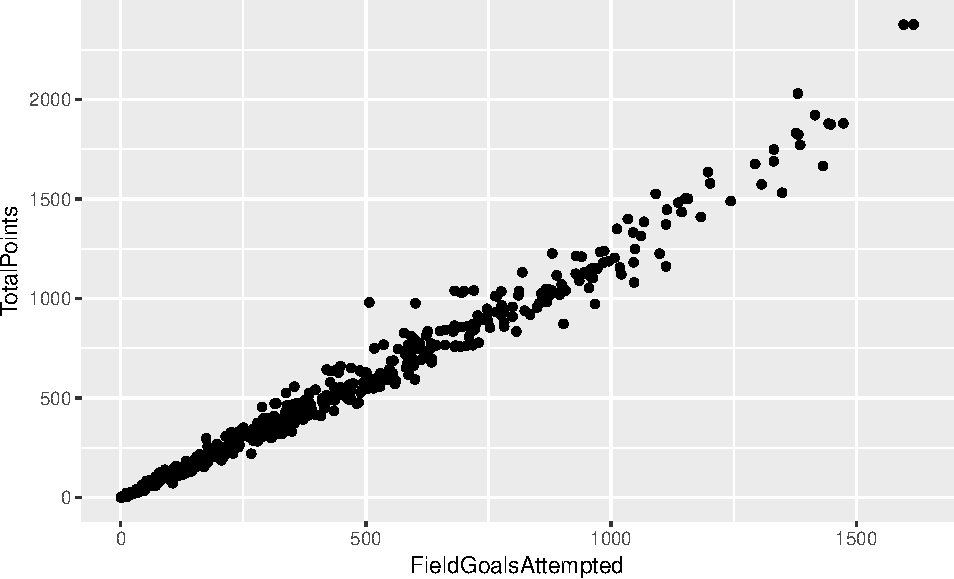
\includegraphics{DataAnalyticsWithR_files/figure-latex/qplot1-1.pdf}

針對做圖的文法的第一個主要元素\textbf{Aesthetics}(包括顏色、形狀、點的大小與線的粗細等),可透過增加指令做修改,如加上\texttt{color=Position},表示用守備位置Position著色

\begin{Shaded}
\begin{Highlighting}[]
\KeywordTok{qplot}\NormalTok{(FieldGoalsAttempted, TotalPoints, }\DataTypeTok{data =} \NormalTok{NBA1516,}\DataTypeTok{color=}\NormalTok{Position)}
\end{Highlighting}
\end{Shaded}

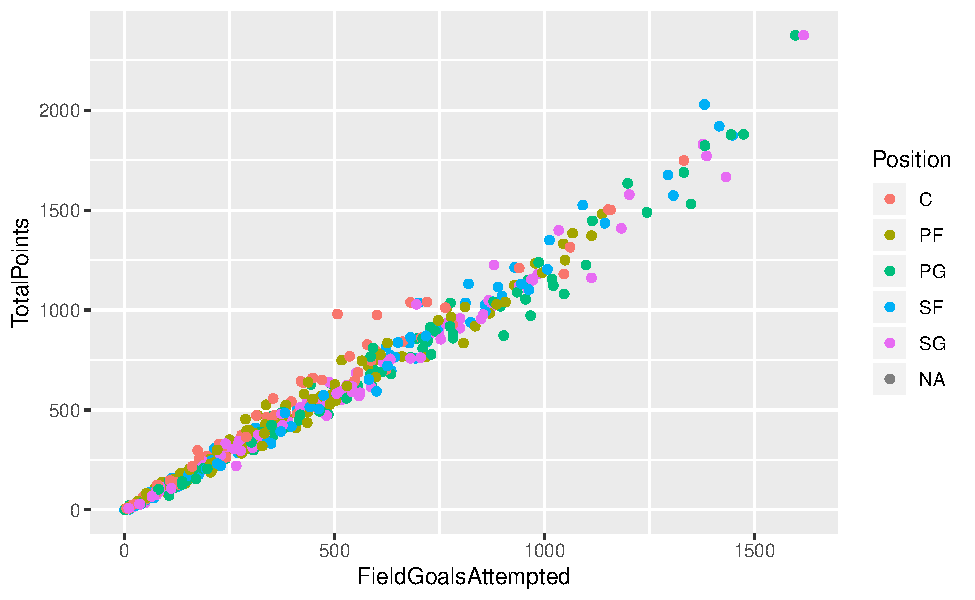
\includegraphics{DataAnalyticsWithR_files/figure-latex/qplot2-1.pdf}
針對做圖的文法的第二個主要元素\textbf{Geometric}(包括點、線、盒狀圖、直條圖等),也可透過增加指令修改,如使用\texttt{geom\ =\ c("point",\ "smooth")}
在圖上加點與漸進線

\begin{Shaded}
\begin{Highlighting}[]
\KeywordTok{qplot}\NormalTok{(FieldGoalsAttempted, TotalPoints, }\DataTypeTok{data =} \NormalTok{NBA1516,}
      \DataTypeTok{geom =} \KeywordTok{c}\NormalTok{(}\StringTok{"point"}\NormalTok{, }\StringTok{"smooth"}\NormalTok{))}
\end{Highlighting}
\end{Shaded}

\begin{verbatim}
## `geom_smooth()` using method = 'loess'
\end{verbatim}

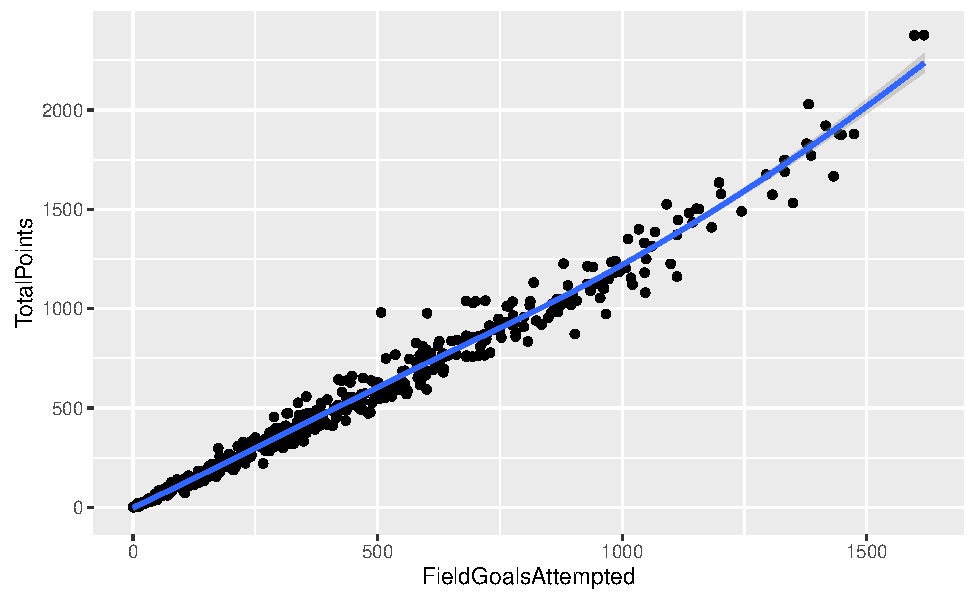
\includegraphics{DataAnalyticsWithR_files/figure-latex/qplot3-1.pdf}

如果輸入的變量並非\textbf{雙}變量,而是\textbf{單}變量時,預設圖形會從\textbf{散佈圖}變為\textbf{Histograms直方圖}

\begin{Shaded}
\begin{Highlighting}[]
\CommentTok{#畫TotalPoints的直方圖/ fill = Position 並用守備位置Position著色}
\KeywordTok{qplot}\NormalTok{(TotalPoints, }\DataTypeTok{data =} \NormalTok{NBA1516, }\DataTypeTok{fill =} \NormalTok{Position)}
\end{Highlighting}
\end{Shaded}

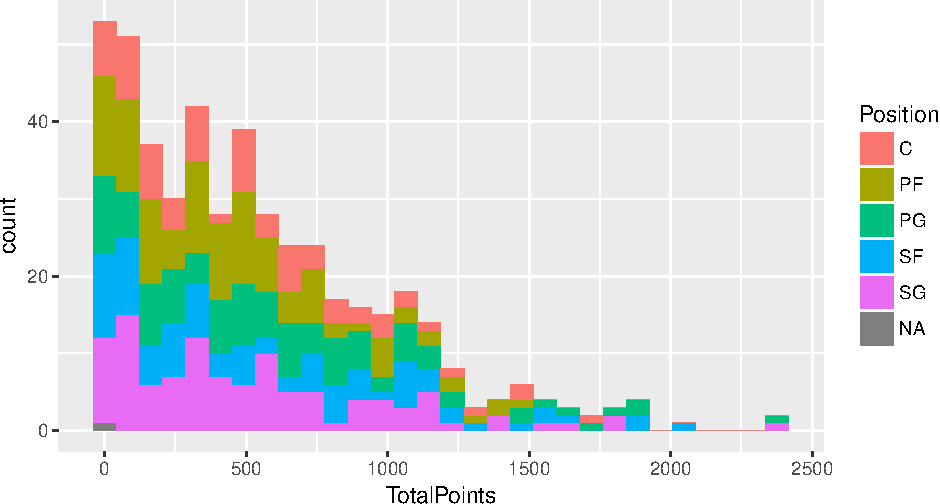
\includegraphics{DataAnalyticsWithR_files/figure-latex/unnamed-chunk-114-1.pdf}

作圖的\textbf{Facets}元素可提供在同一張圖內做多個子圖的方法,只要使用\texttt{facets\ =}來設定子圖分類的依據參數即可,以下圖為例,輸入的變量是\textbf{雙}變量,所以預設圖形為散佈圖,而設定子圖的語法為\texttt{直向分類\textasciitilde{}橫向分類},直向分類意指以增加列(Row)的方式畫子圖,橫向分類意指以增加行(Column)的方式畫子圖,通常只會設定單一方向,如果選擇的是\texttt{直向},\texttt{橫向分類}部分可用\texttt{.}表示,範例如下:

\begin{Shaded}
\begin{Highlighting}[]
\CommentTok{#facets = . ~ Position 用守備位置Position分群畫圖(橫向)}
\KeywordTok{qplot}\NormalTok{(FieldGoalsAttempted, TotalPoints, }
      \DataTypeTok{data =} \NormalTok{NBA1516,}
      \DataTypeTok{facets =} \NormalTok{. ~}\StringTok{ }\NormalTok{Position)}
\end{Highlighting}
\end{Shaded}

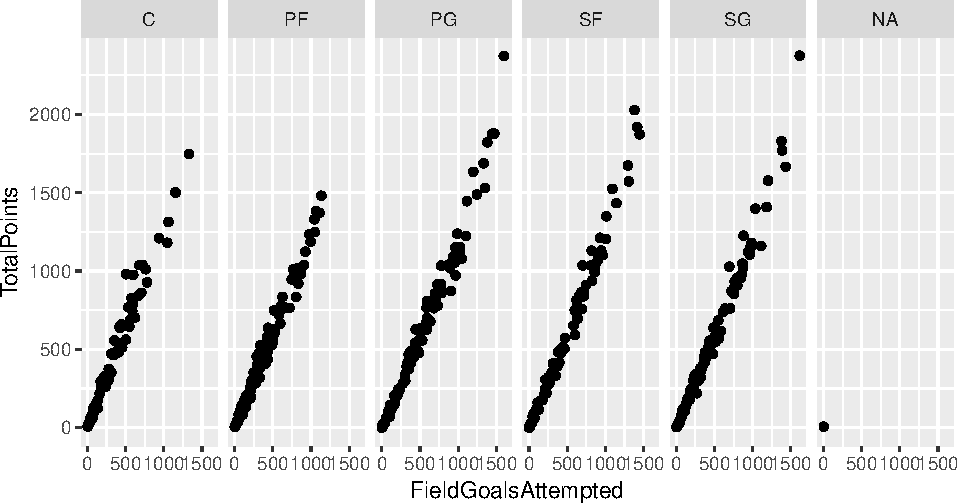
\includegraphics{DataAnalyticsWithR_files/figure-latex/unnamed-chunk-115-1.pdf}

\begin{Shaded}
\begin{Highlighting}[]
\CommentTok{#facets = . ~ Position 用守備位置Position分群畫圖(直向)}
\KeywordTok{qplot}\NormalTok{(FieldGoalsAttempted, TotalPoints, }
      \DataTypeTok{data =} \NormalTok{NBA1516,}
      \DataTypeTok{facets =} \NormalTok{Position ~}\StringTok{ }\NormalTok{.)}
\end{Highlighting}
\end{Shaded}

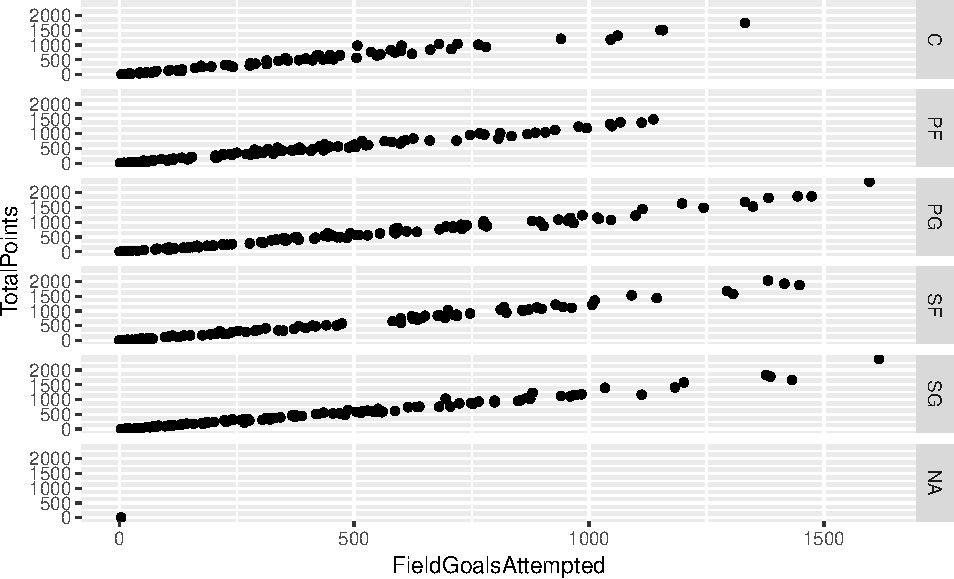
\includegraphics{DataAnalyticsWithR_files/figure-latex/unnamed-chunk-116-1.pdf}

\texttt{ggplot2}套件會自動幫使用者選擇顏色與圖形各項參數,但使用者也可依需求微調,如直方圖的分組間隔,可透過\texttt{binwidth}參數設定

\begin{Shaded}
\begin{Highlighting}[]
\CommentTok{#facets = . ~ Position 用守備位置Position分群畫圖(直向)}
\NormalTok{##binwidth = 2 每2分一組}
\KeywordTok{qplot}\NormalTok{(TotalPoints, }\DataTypeTok{data =} \NormalTok{NBA1516, }
      \DataTypeTok{facets =} \NormalTok{Position ~}\StringTok{ }\NormalTok{., }\DataTypeTok{binwidth =} \DecValTok{2}\NormalTok{)}
\end{Highlighting}
\end{Shaded}

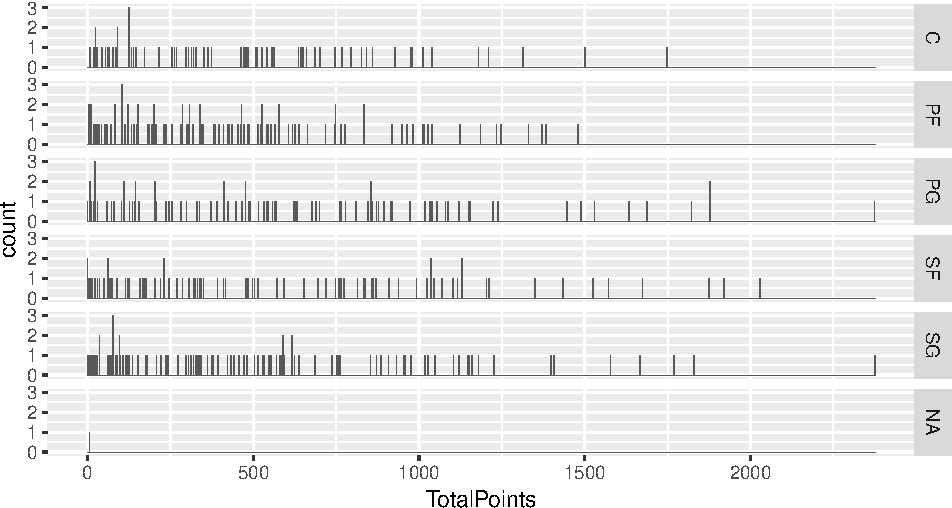
\includegraphics{DataAnalyticsWithR_files/figure-latex/unnamed-chunk-117-1.pdf}

\begin{Shaded}
\begin{Highlighting}[]
\CommentTok{#facets = . ~ Position 用守備位置Position分群畫圖(直向)}
\NormalTok{##binwidth = 100 每100分一組}
\KeywordTok{qplot}\NormalTok{(TotalPoints, }\DataTypeTok{data =} \NormalTok{NBA1516,}
      \DataTypeTok{facets =} \NormalTok{Position ~}\StringTok{ }\NormalTok{., }\DataTypeTok{binwidth =} \DecValTok{100}\NormalTok{)}
\end{Highlighting}
\end{Shaded}

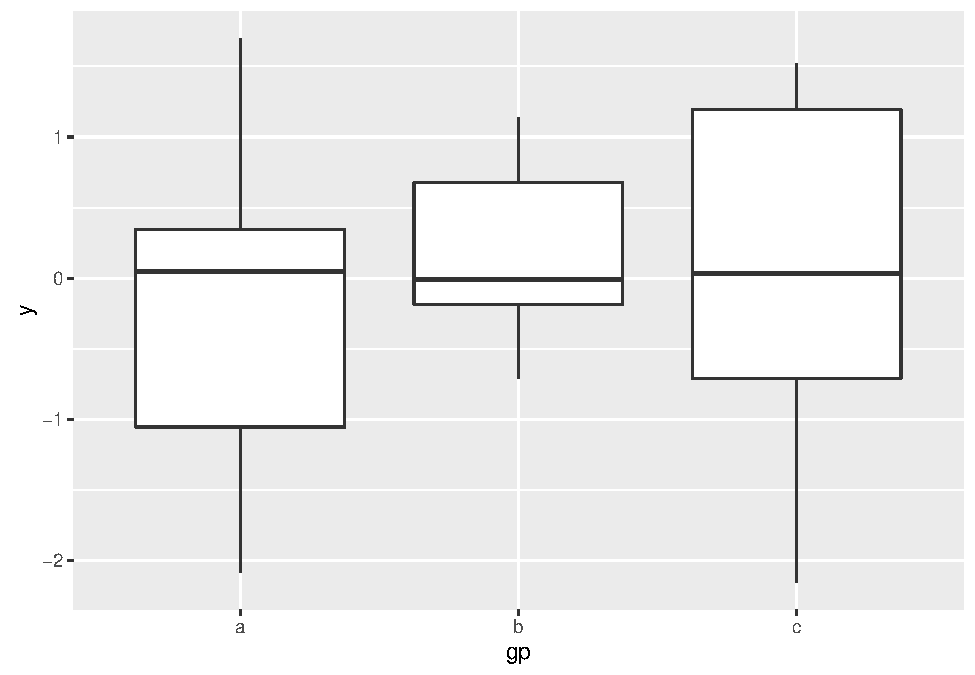
\includegraphics{DataAnalyticsWithR_files/figure-latex/unnamed-chunk-118-1.pdf}

總括來說\texttt{qplot()}提供快速方便的畫圖功能,並且保留部分參數設定的彈性,但若需要調整更多參數,仍須使用完整的\texttt{ggplot()}函式。

\subsection{ggplot()}\label{ggplot}

使用ggplot2作圖有以下步驟:

\begin{itemize}
\tightlist
\item
  準備好資料。當然要有資料才能畫圖
\item
  設定\textbf{Aesthetic attributes}。使用\texttt{aes(x,\ y,\ ...)}指定
\item
  指定\textbf{Geometric
  objects}。常用的包括\texttt{geom\_point()}、\texttt{geom\_line()}、\texttt{geom\_point()}、\texttt{geom\_polygon()}、\texttt{geom\_errorbar()}
\end{itemize}

\begin{Shaded}
\begin{Highlighting}[]
\KeywordTok{library}\NormalTok{(ggplot2) ##須先安裝 install.packages("ggplot2")}
\end{Highlighting}
\end{Shaded}

首先先產生教學用畫圖資料

\begin{Shaded}
\begin{Highlighting}[]
\NormalTok{df <-}\StringTok{ }\KeywordTok{data.frame}\NormalTok{(}\DataTypeTok{gp =} \KeywordTok{factor}\NormalTok{(}\KeywordTok{rep}\NormalTok{(letters[}\DecValTok{1}\NormalTok{:}\DecValTok{3}\NormalTok{], }\DataTypeTok{each =} \DecValTok{10}\NormalTok{)),}\DataTypeTok{y =} \KeywordTok{rnorm}\NormalTok{(}\DecValTok{30}\NormalTok{))}
\end{Highlighting}
\end{Shaded}

設定兩個畫圖的重要元素\textbf{Aesthetic attributes}和\textbf{Geometric
objects}

\begin{Shaded}
\begin{Highlighting}[]
\KeywordTok{ggplot}\NormalTok{(df, }\KeywordTok{aes}\NormalTok{(}\DataTypeTok{x =} \NormalTok{gp, }\DataTypeTok{y =} \NormalTok{y)) +}\KeywordTok{geom_point}\NormalTok{()}
\end{Highlighting}
\end{Shaded}

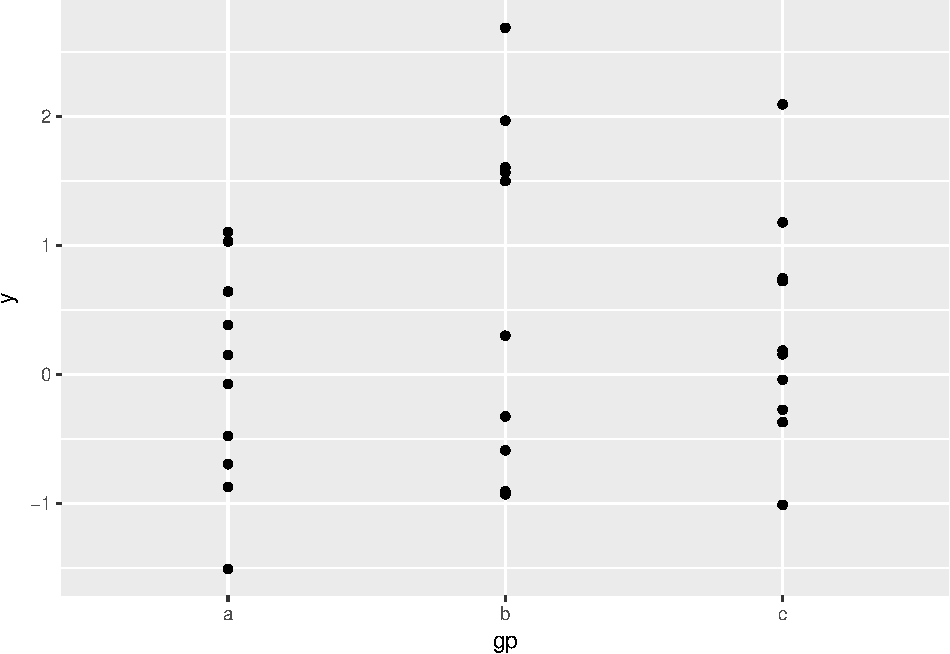
\includegraphics{DataAnalyticsWithR_files/figure-latex/unnamed-chunk-121-1.pdf}
用\texttt{geom\_boxpolt()}改畫盒狀圖

\begin{Shaded}
\begin{Highlighting}[]
\KeywordTok{ggplot}\NormalTok{(df, }\KeywordTok{aes}\NormalTok{(}\DataTypeTok{x =} \NormalTok{gp, }\DataTypeTok{y =} \NormalTok{y)) +}\KeywordTok{geom_boxplot}\NormalTok{()}
\end{Highlighting}
\end{Shaded}

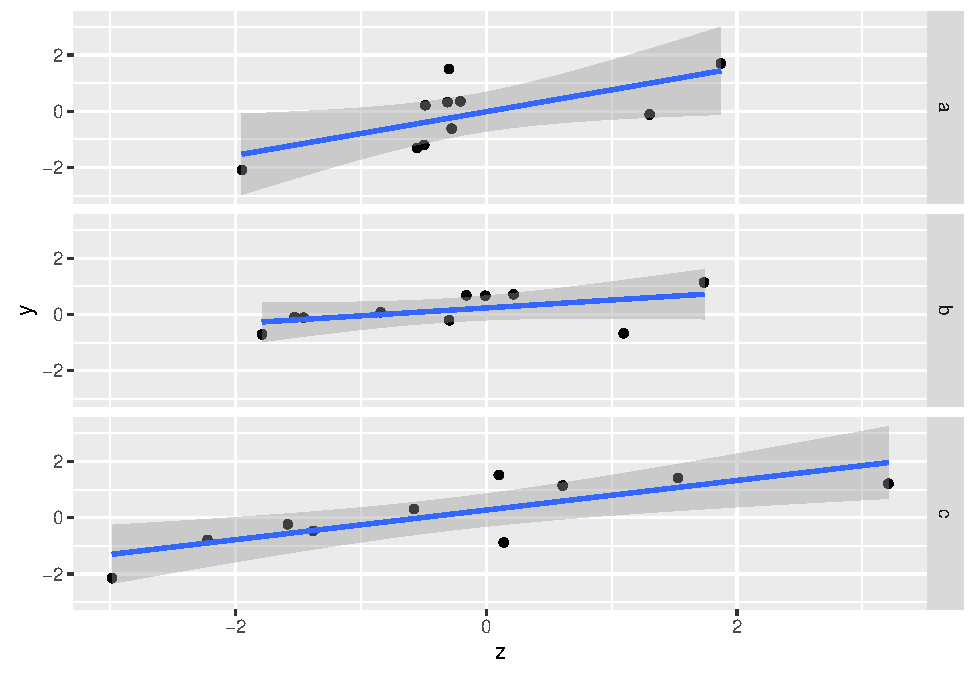
\includegraphics{DataAnalyticsWithR_files/figure-latex/unnamed-chunk-122-1.pdf}
使用Faceting功能

\begin{Shaded}
\begin{Highlighting}[]
\NormalTok{df$z<-df$y+}\KeywordTok{rnorm}\NormalTok{(}\DecValTok{30}\NormalTok{)}
\KeywordTok{ggplot}\NormalTok{(df, }\KeywordTok{aes}\NormalTok{(}\DataTypeTok{x =} \NormalTok{z, }\DataTypeTok{y =} \NormalTok{y)) +}\KeywordTok{geom_point}\NormalTok{()+}\KeywordTok{facet_grid}\NormalTok{(gp~.)}
\end{Highlighting}
\end{Shaded}

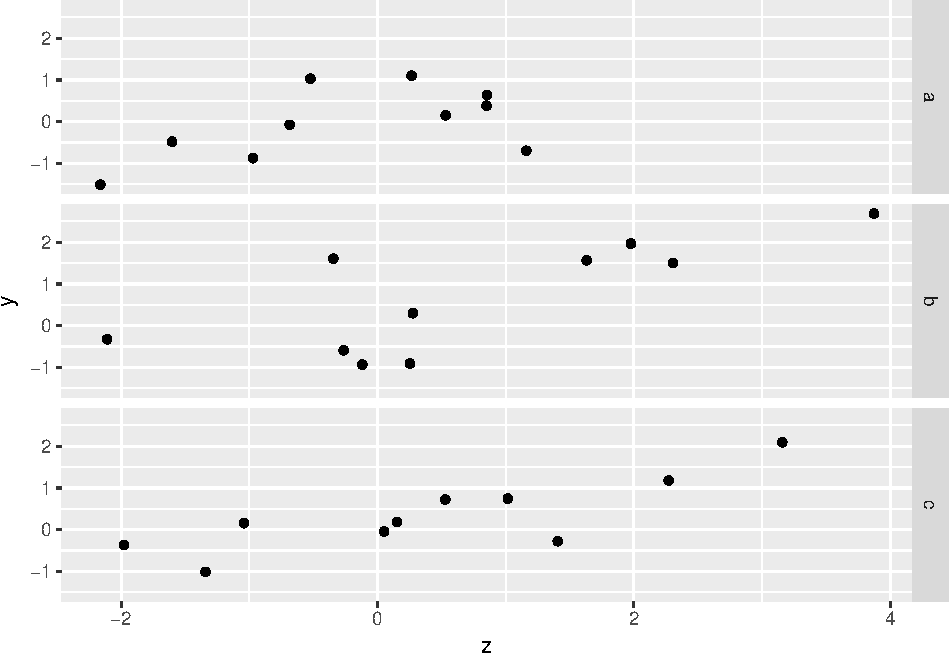
\includegraphics{DataAnalyticsWithR_files/figure-latex/unnamed-chunk-123-1.pdf}
轉向

\begin{Shaded}
\begin{Highlighting}[]
\KeywordTok{ggplot}\NormalTok{(df, }\KeywordTok{aes}\NormalTok{(}\DataTypeTok{x =} \NormalTok{z, }\DataTypeTok{y =} \NormalTok{y)) +}\KeywordTok{geom_point}\NormalTok{()+}\KeywordTok{facet_grid}\NormalTok{(.~gp)}
\end{Highlighting}
\end{Shaded}

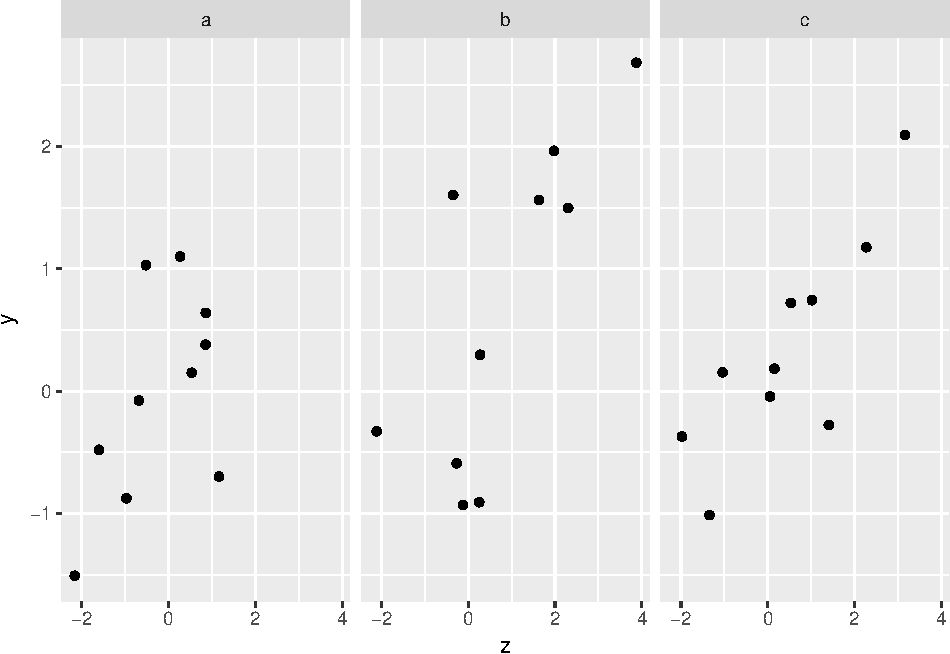
\includegraphics{DataAnalyticsWithR_files/figure-latex/unnamed-chunk-124-1.pdf}
用\texttt{geom\_smooth()}替xy散佈圖加上趨勢線

\begin{Shaded}
\begin{Highlighting}[]
\KeywordTok{ggplot}\NormalTok{(df, }\KeywordTok{aes}\NormalTok{(}\DataTypeTok{x =} \NormalTok{z, }\DataTypeTok{y =} \NormalTok{y)) +}\KeywordTok{geom_point}\NormalTok{()+}\KeywordTok{facet_grid}\NormalTok{(gp~.)+}\KeywordTok{geom_smooth}\NormalTok{()}
\end{Highlighting}
\end{Shaded}

\begin{verbatim}
## `geom_smooth()` using method = 'loess'
\end{verbatim}

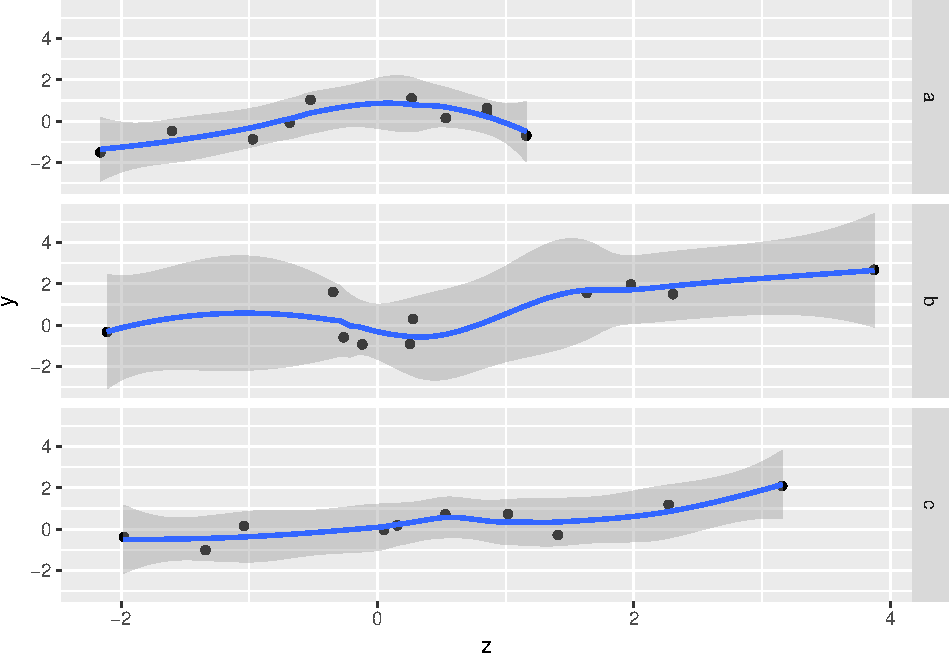
\includegraphics{DataAnalyticsWithR_files/figure-latex/unnamed-chunk-125-1.pdf}
用\texttt{geom\_smooth()}替xy散佈圖加上趨勢線,使用linear regresion

\begin{Shaded}
\begin{Highlighting}[]
\KeywordTok{ggplot}\NormalTok{(df, }\KeywordTok{aes}\NormalTok{(}\DataTypeTok{x =} \NormalTok{z, }\DataTypeTok{y =} \NormalTok{y)) +}\KeywordTok{geom_point}\NormalTok{()+}\KeywordTok{facet_grid}\NormalTok{(gp~.)+}\KeywordTok{geom_smooth}\NormalTok{(}\DataTypeTok{method=}\StringTok{'lm'}\NormalTok{)}
\end{Highlighting}
\end{Shaded}

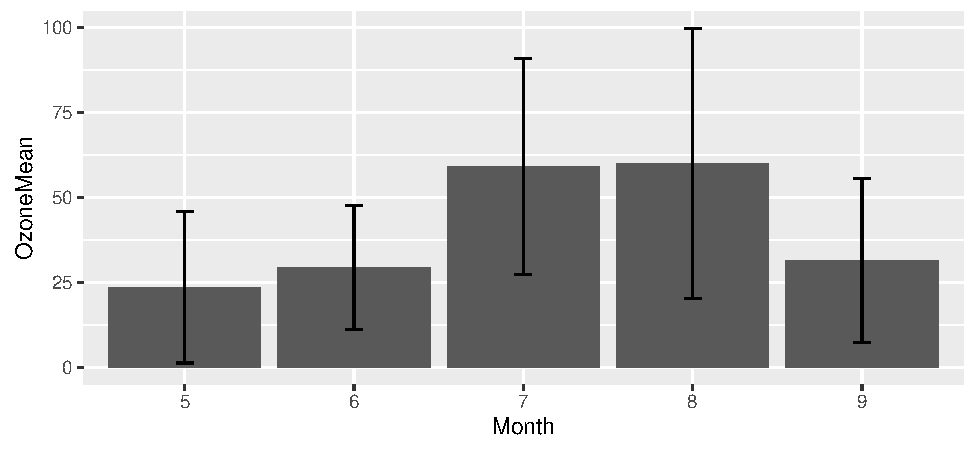
\includegraphics{DataAnalyticsWithR_files/figure-latex/unnamed-chunk-126-1.pdf}
改用\texttt{geom\_line()}畫線

\begin{Shaded}
\begin{Highlighting}[]
\KeywordTok{ggplot}\NormalTok{(df, }\KeywordTok{aes}\NormalTok{(}\DataTypeTok{x =} \NormalTok{z, }\DataTypeTok{y =} \NormalTok{y)) +}\KeywordTok{geom_line}\NormalTok{()+}\KeywordTok{facet_grid}\NormalTok{(gp~.)}
\end{Highlighting}
\end{Shaded}

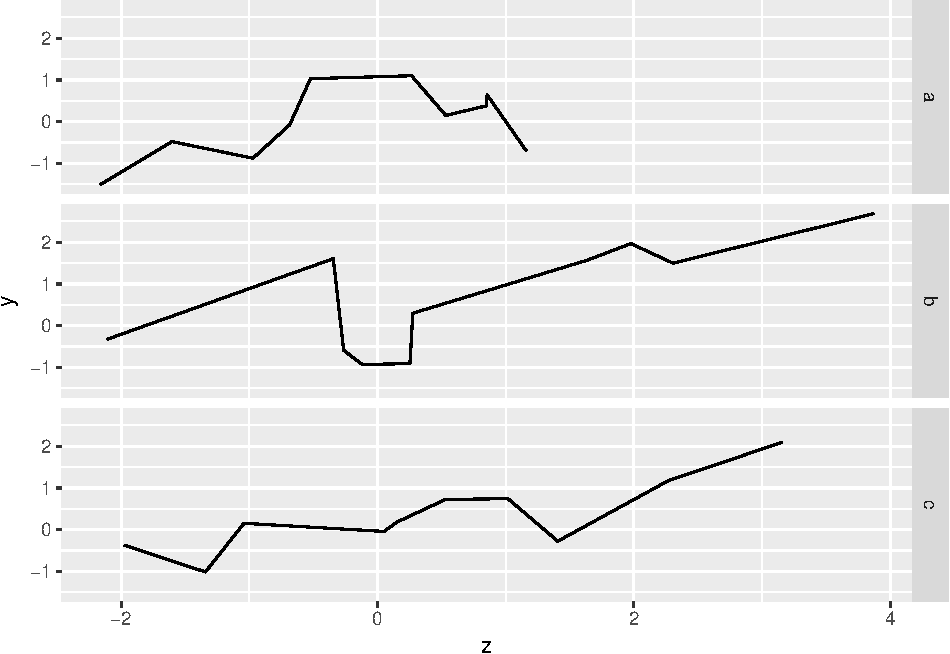
\includegraphics{DataAnalyticsWithR_files/figure-latex/unnamed-chunk-127-1.pdf}
改用顏色分組,使用\texttt{aes(color=\textquotesingle{}group\ name\textquotesingle{})}

\begin{Shaded}
\begin{Highlighting}[]
\KeywordTok{ggplot}\NormalTok{(df, }\KeywordTok{aes}\NormalTok{(}\DataTypeTok{x =} \NormalTok{z, }\DataTypeTok{y =} \NormalTok{y, }\DataTypeTok{color=}\NormalTok{gp)) +}\KeywordTok{geom_line}\NormalTok{()}
\end{Highlighting}
\end{Shaded}

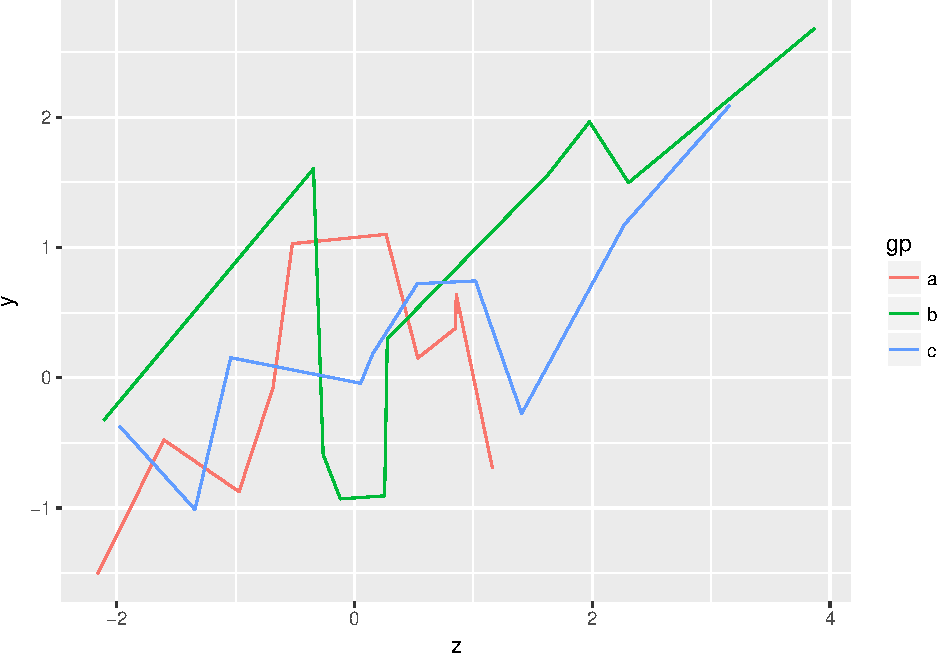
\includegraphics{DataAnalyticsWithR_files/figure-latex/unnamed-chunk-128-1.pdf}

畫圖前需要注意的幾個小地方:

提供資料時,把資料修改為想要在圖片顯示的文字。從上面的範例可以發現,ggplot2會直接將資料分組(a/b/c)直接標在圖上,與其之後再來改圖,不如在資料處理時就將a/b/c改為有意義且可以直接使用的文字。
如果是離散性的資料,但卻又是數值時(像是1,2,3)可以用factor()轉換,ggplot會將factor視為離散資料。

除了基本的製圖外,\texttt{ggplot2}套件也提供完整的資料標示設定與其他參數設定功能,包括:

\begin{itemize}
\tightlist
\item
  標籤 \texttt{xlab()}, \texttt{ylab()}, \texttt{labs(x=,y=)},
  \texttt{ggtitle()}
\item
  每一個\texttt{geom\_*()}都有參數可設定
\item
  圖形樣式設定 \texttt{theme()},可使用內建樣式
\item
  \texttt{theme\_gray()}: 灰背景,預設樣式
\item
  \texttt{theme\_bw()}: 黑白樣式
\item
  使用其他樣式套件
\item
  \texttt{ggthemes} packages
  \href{https://cran.r-project.org/web/packages/ggthemes/vignettes/ggthemes.html}{Website}
\item
  \texttt{xkcd} packages
  \href{http://xkcd.r-forge.r-project.org/}{Website}
\end{itemize}

在比較多組的平均值高低時,因為各組樣本數與資料分佈不同,平均數的誤差值也會不同,所以在資料視覺化時,建議加上誤差線(Error
bar),誤差線通常使用在bar chart和line
chart,而誤差值的計算有下列三種選擇:

\begin{itemize}
\tightlist
\item
  Standard deviation (SD) 標準差:呈現資料本質時使用
\item
  Standard error (SE) 標準誤差:呈現預估平均值的可能誤差時使用
\item
  Confidence interval (CI) 信賴區間:呈現預估平均值的信心時使用
\end{itemize}

以空氣污染料為例,若想比較各月臭氧濃度差異,可以使用bar
chart來呈現,在ggplot2中,如果要畫bar chart,需要將\textbf{Geometric
objects}設定為\texttt{geom\_bar}

\begin{Shaded}
\begin{Highlighting}[]
\KeywordTok{library}\NormalTok{(datasets) }
\KeywordTok{library}\NormalTok{(data.table)}
\NormalTok{airquality$Month<-}\KeywordTok{as.factor}\NormalTok{(airquality$Month) }\CommentTok{#將Month轉為因子變項}
\NormalTok{airquality.mean<-}\KeywordTok{data.table}\NormalTok{(airquality)[,.(}\DataTypeTok{OzoneMean=}\KeywordTok{mean}\NormalTok{(Ozone,}\DataTypeTok{na.rm =} \NormalTok{T)),by=Month] }\CommentTok{#計算每月Ozone平均}
\KeywordTok{ggplot}\NormalTok{()+}\KeywordTok{geom_bar}\NormalTok{(}\DataTypeTok{data=}\NormalTok{airquality.mean,}\KeywordTok{aes}\NormalTok{(}\DataTypeTok{x=}\NormalTok{Month,}\DataTypeTok{y=}\NormalTok{OzoneMean),}
                  \DataTypeTok{stat =} \StringTok{"identity"}\NormalTok{) }\CommentTok{#stat = "identity" 直接畫數字}
\end{Highlighting}
\end{Shaded}

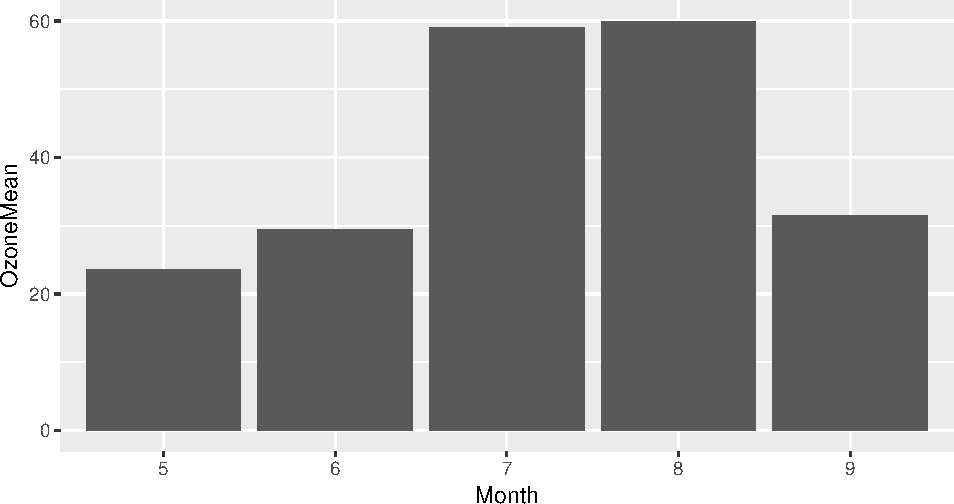
\includegraphics{DataAnalyticsWithR_files/figure-latex/unnamed-chunk-129-1.pdf}

在ggplot2套件中,只要加上\texttt{geom\_errorbar()}函式,設定資料高低值,就能在原圖中加上誤差線

\begin{Shaded}
\begin{Highlighting}[]
\KeywordTok{library}\NormalTok{(datasets) }
\KeywordTok{library}\NormalTok{(data.table)}
\NormalTok{airquality$Month<-}\KeywordTok{as.factor}\NormalTok{(airquality$Month) }\CommentTok{#將Month轉為因子變項}
\NormalTok{airquality.stat<-}\KeywordTok{data.table}\NormalTok{(airquality)[,.(}\DataTypeTok{OzoneMean=}\KeywordTok{mean}\NormalTok{(Ozone,}\DataTypeTok{na.rm =} \NormalTok{T),}\DataTypeTok{OzoneSD=}\KeywordTok{sd}\NormalTok{(Ozone,}\DataTypeTok{na.rm =} \NormalTok{T)),by=Month] }\CommentTok{#計算每月Ozone平均與標準差}
\KeywordTok{ggplot}\NormalTok{(}\DataTypeTok{data=}\NormalTok{airquality.stat)+}\StringTok{ }\CommentTok{#資料airquality.eb}
\StringTok{    }\KeywordTok{geom_bar}\NormalTok{(}\KeywordTok{aes}\NormalTok{(}\DataTypeTok{x=}\NormalTok{Month,}\DataTypeTok{y=}\NormalTok{OzoneMean),}\DataTypeTok{stat =} \StringTok{"identity"}\NormalTok{)+}
\StringTok{    }\KeywordTok{geom_errorbar}\NormalTok{( }\CommentTok{#ymin低點, ymax高點}
        \KeywordTok{aes}\NormalTok{(}\DataTypeTok{x=}\NormalTok{Month,}\DataTypeTok{ymin=}\NormalTok{OzoneMean-OzoneSD,}\DataTypeTok{ymax=}\NormalTok{OzoneMean+OzoneSD), }\DataTypeTok{width=}\NormalTok{.}\DecValTok{1}\NormalTok{)}
\end{Highlighting}
\end{Shaded}

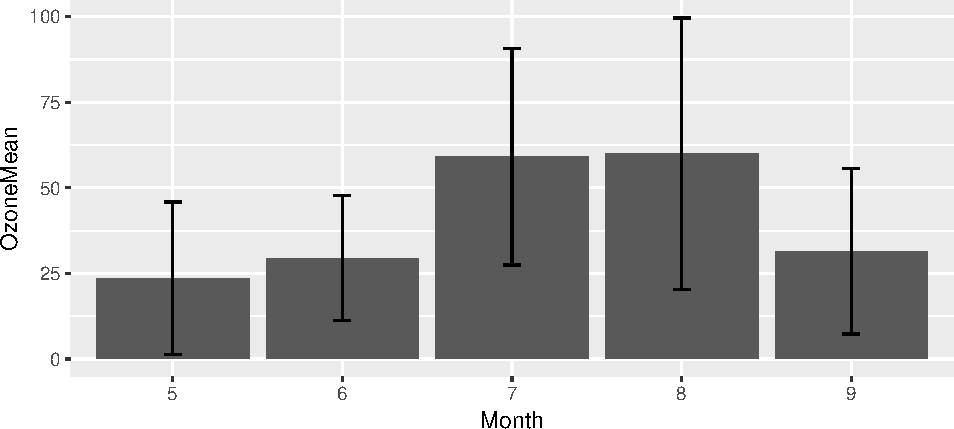
\includegraphics{DataAnalyticsWithR_files/figure-latex/unnamed-chunk-130-1.pdf}

\section{ggplot2+地圖}\label{ggplot2}

\subsection{Choropleth map面量圖}\label{choropleth-map}

Choropleth
map\href{https://en.wikipedia.org/wiki/Choropleth_map}{面量圖}是指\textbf{把統計資料用顏色畫在對應的地圖上}的一種資料視覺化方式,在R中可以使用\texttt{choroplethr}\citep{R-choroplethr}
package來畫面量圖, \texttt{choroplethr}
package是一個基於\texttt{ggplot2}
package的\texttt{面量圖}做圖工具,使用前需要先安裝,建議同時安裝\texttt{choroplethrMaps}
package

\begin{Shaded}
\begin{Highlighting}[]
\KeywordTok{install.packages}\NormalTok{(}\KeywordTok{c}\NormalTok{(}\StringTok{"choroplethr"}\NormalTok{,}\StringTok{"choroplethrMaps"}\NormalTok{)) ##第一次使用前先安裝}
\end{Highlighting}
\end{Shaded}

\begin{Shaded}
\begin{Highlighting}[]
\KeywordTok{library}\NormalTok{(choroplethr)}
\end{Highlighting}
\end{Shaded}

\texttt{choroplethr}\citep{R-choroplethr}
package內建美國各州地圖與人口學資料,所以可以輕鬆使用\texttt{state\_choropleth()}函式畫出美國各州人口分布

\begin{Shaded}
\begin{Highlighting}[]
\KeywordTok{data}\NormalTok{(df_pop_state) }\CommentTok{#記載各州人口數的資料}
\KeywordTok{state_choropleth}\NormalTok{(df_pop_state) }\CommentTok{#把各州人口畫在地圖上}
\end{Highlighting}
\end{Shaded}

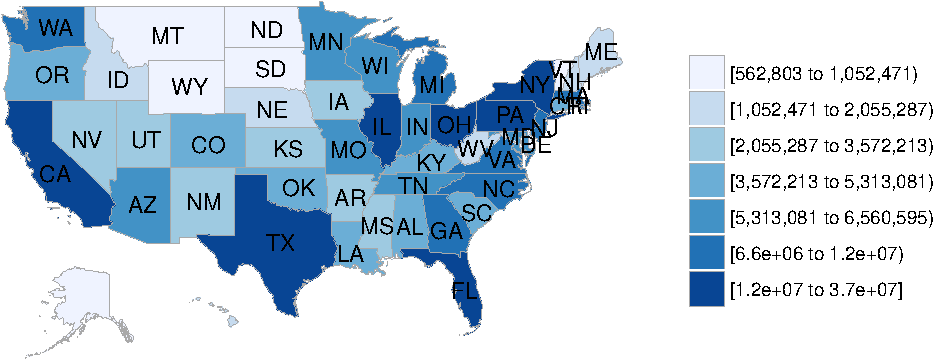
\includegraphics{DataAnalyticsWithR_files/figure-latex/unnamed-chunk-133-1.pdf}
若在將\texttt{reference\_map}設定為\texttt{=\ TRUE},可在面量圖的背景加上google地圖

\begin{Shaded}
\begin{Highlighting}[]
\KeywordTok{data}\NormalTok{(continental_us_states)}
\KeywordTok{state_choropleth}\NormalTok{(df_pop_state,}\DataTypeTok{reference_map =} \OtherTok{TRUE}\NormalTok{,}
                 \DataTypeTok{zoom=} \NormalTok{continental_us_states) }\CommentTok{#把各州人口畫在地圖上}
\end{Highlighting}
\end{Shaded}

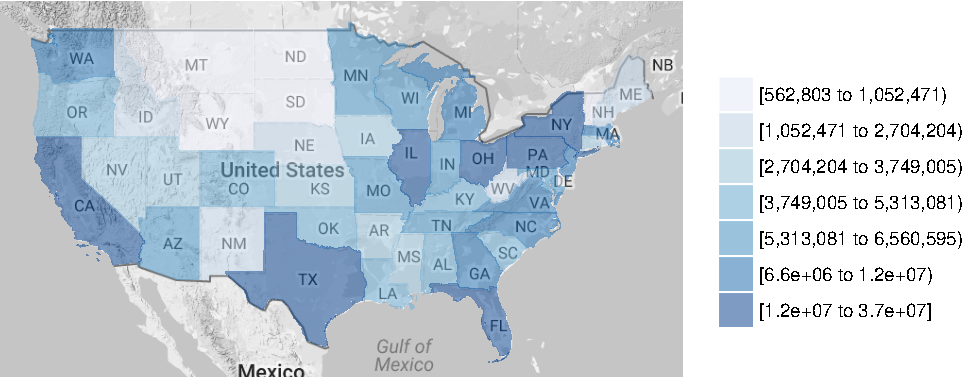
\includegraphics{DataAnalyticsWithR_files/figure-latex/unnamed-chunk-134-1.pdf}

除了美國地圖外,使用\texttt{choroplethr} package搭配\texttt{WDI}:
\href{http://beta.data.worldbank.org/}{World Development Indicators}
的世界人口分布資料,可以針對世界人口分佈做\textbf{面量圖}。
世界人口資料的代碼為\texttt{SP.POP.TOTL},代碼查詢可見\href{http://beta.data.worldbank.org/}{World
Development Indicators}

由於需要使用\texttt{WDI}的資料,所以需要安裝與載入\texttt{WDI}\citep{R-WDI}
package

\begin{Shaded}
\begin{Highlighting}[]
\KeywordTok{install.packages}\NormalTok{(}\StringTok{"WDI"}\NormalTok{) ##第一次使用前先安裝}
\end{Highlighting}
\end{Shaded}

\begin{Shaded}
\begin{Highlighting}[]
\KeywordTok{library}\NormalTok{(WDI)}
\KeywordTok{choroplethr_wdi}\NormalTok{(}\DataTypeTok{code=}\StringTok{"SP.POP.TOTL"}\NormalTok{, }\DataTypeTok{year=}\DecValTok{2014}\NormalTok{, }
                \DataTypeTok{title=}\StringTok{"2015 Population"}\NormalTok{, }\DataTypeTok{num_colors=}\DecValTok{1}\NormalTok{)}
\end{Highlighting}
\end{Shaded}

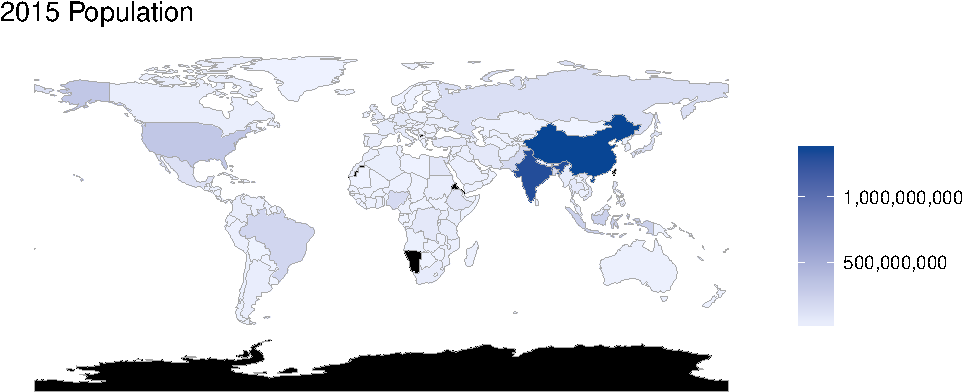
\includegraphics{DataAnalyticsWithR_files/figure-latex/choroplethr_wdi_1 -1.pdf}

除了人口資料外,WDI也有世界平均壽命資料,平均壽命的代碼為\texttt{SP.DYN.LE00.IN},代碼查詢可見\href{http://beta.data.worldbank.org/}{World
Development Indicators}

\begin{Shaded}
\begin{Highlighting}[]
\KeywordTok{choroplethr_wdi}\NormalTok{(}\DataTypeTok{code=}\StringTok{"SP.DYN.LE00.IN"}\NormalTok{, }\DataTypeTok{year=}\DecValTok{2014}\NormalTok{, }
                \DataTypeTok{title=}\StringTok{"2014 Life Expectancy"}\NormalTok{)}
\end{Highlighting}
\end{Shaded}

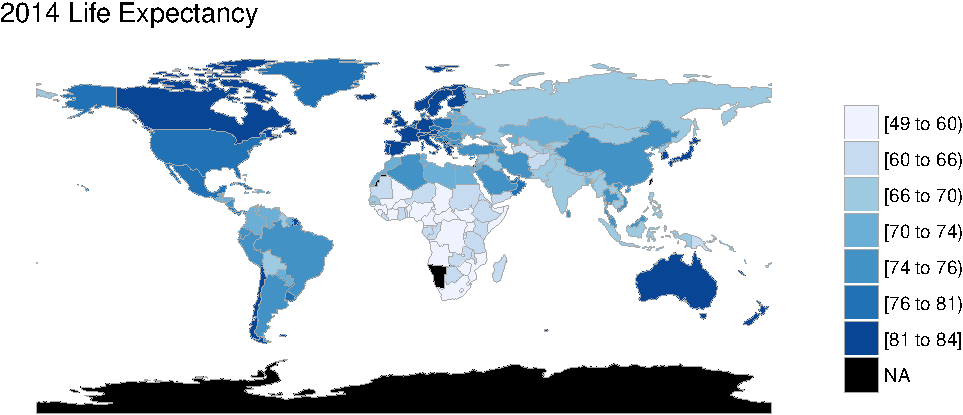
\includegraphics{DataAnalyticsWithR_files/figure-latex/choroplethr_wdi_2-1.pdf}

如果只需亞洲太平洋人口分布,可使用\texttt{zoom}參數設定想畫的國家,國家的名稱設定必須要和\texttt{country.regions}資料完全吻合

\begin{Shaded}
\begin{Highlighting}[]
\KeywordTok{choroplethr_wdi}\NormalTok{(}\DataTypeTok{code=}\StringTok{"SP.POP.TOTL"}\NormalTok{, }\DataTypeTok{year=}\DecValTok{2015}\NormalTok{, }
                \DataTypeTok{title=}\StringTok{"2015 Life Expectancy"}\NormalTok{,}
                \DataTypeTok{zoom=}\KeywordTok{c}\NormalTok{(}\StringTok{'taiwan'}\NormalTok{,}\StringTok{'japan'}\NormalTok{,}\StringTok{'south korea'}\NormalTok{,}\StringTok{'philippines'}\NormalTok{))}
\end{Highlighting}
\end{Shaded}

\subsection{ggmap()}\label{ggmap}

\texttt{ggmap}\citep{R-ggmap} package是一個可以把google
map載入並作圖的套件,一樣是基於\texttt{ggplot2}套件開發的。
依照往例,第一次使用前需要安裝

\begin{Shaded}
\begin{Highlighting}[]
\KeywordTok{install.packages}\NormalTok{(}\StringTok{"ggmap"}\NormalTok{, }\DataTypeTok{type =} \StringTok{"source"}\NormalTok{) ##第一次使用前先安裝}
\end{Highlighting}
\end{Shaded}

載入\texttt{ggmap}\citep{R-ggmap}
package後,可以使用\texttt{get\_map()}函式取得google
map圖層,並用\texttt{ggmap()}函式將取得的圖層畫出來,\texttt{get\_map()}函式需要設定的參數如下:

\begin{itemize}
\tightlist
\item
  location 地點,可以是地名,也可以是經緯度座標
\item
  zoom 放大倍率
\item
  language 地圖語言
\end{itemize}

\begin{Shaded}
\begin{Highlighting}[]
\KeywordTok{library}\NormalTok{(ggmap)}
\NormalTok{twmap <-}\StringTok{ }\KeywordTok{get_map}\NormalTok{(}\DataTypeTok{location =} \StringTok{'Taiwan'}\NormalTok{, }\DataTypeTok{zoom =} \DecValTok{7}\NormalTok{,}\DataTypeTok{language =} \StringTok{"zh-TW"}\NormalTok{)}
\KeywordTok{ggmap}\NormalTok{(twmap)}
\end{Highlighting}
\end{Shaded}

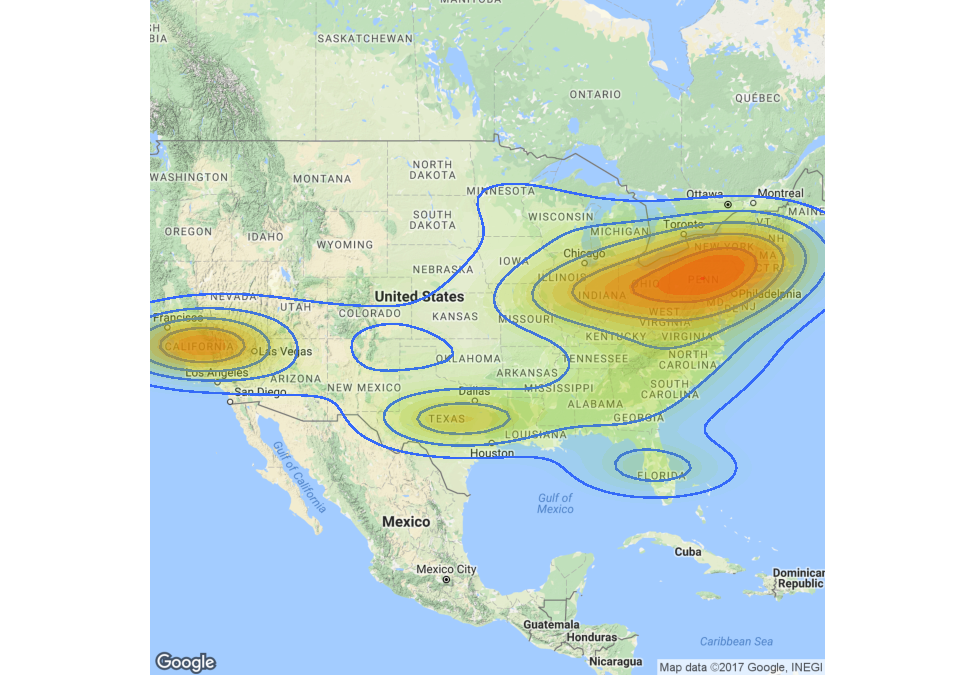
\includegraphics{DataAnalyticsWithR_files/figure-latex/unnamed-chunk-137-1.pdf}

只要資料有經緯度等資訊,就可以使用\texttt{ggmap}
package與各式資料結合呈現,以台北市水質地圖開放資料為例,首先先將資料載入處理(參考Ch
\ref{JSON})。台北市水質資料的Open data
API網址是http://data.taipei/opendata/datalist/apiAccess?scope=resourceAquire\&rid=190796c8-7c56-42e0-8068-39242b8ec927

\begin{Shaded}
\begin{Highlighting}[]
\NormalTok{##資料載入}
\KeywordTok{library}\NormalTok{(jsonlite)}
\KeywordTok{library}\NormalTok{(RCurl)}
\NormalTok{WaterData<-}\KeywordTok{fromJSON}\NormalTok{(}\KeywordTok{getURL}\NormalTok{(}\StringTok{"http://data.taipei/opendata/datalist/apiAccess?scope=resourceAquire&rid=190796c8-7c56-42e0-8068-39242b8ec927"}\NormalTok{))}
\NormalTok{WaterDataFrame<-WaterData$result$results}
\NormalTok{WaterDataFrame$longitude<-}\KeywordTok{as.numeric}\NormalTok{(WaterDataFrame$longitude)}
\NormalTok{WaterDataFrame$latitude<-}\KeywordTok{as.numeric}\NormalTok{(WaterDataFrame$latitude)}
\NormalTok{WaterDataFrame$qua_cntu<-}\KeywordTok{as.numeric}\NormalTok{(WaterDataFrame$qua_cntu)}
\NormalTok{##結合ggmap}
\KeywordTok{library}\NormalTok{(ggmap)}
\NormalTok{TaipeiMap =}\StringTok{ }\KeywordTok{get_map}\NormalTok{(}\DataTypeTok{location =} \KeywordTok{c}\NormalTok{(}\FloatTok{121.43}\NormalTok{,}\FloatTok{24.93}\NormalTok{,}\FloatTok{121.62}\NormalTok{,}\FloatTok{25.19}\NormalTok{), }
                    \DataTypeTok{zoom =} \DecValTok{11}\NormalTok{, }\DataTypeTok{maptype =} \StringTok{'roadmap'}\NormalTok{)}
\NormalTok{TaipeiMapO =}\StringTok{ }\KeywordTok{ggmap}\NormalTok{(TaipeiMap)+}\StringTok{ }
\StringTok{    }\KeywordTok{geom_point}\NormalTok{(}\DataTypeTok{data=}\NormalTok{WaterDataFrame[WaterDataFrame$qua_cntu>=}\DecValTok{0}\NormalTok{,], }
               \KeywordTok{aes}\NormalTok{(}\DataTypeTok{x=}\NormalTok{longitude, }\DataTypeTok{y=}\NormalTok{latitude,}\DataTypeTok{color=}\NormalTok{qua_cntu,}\DataTypeTok{size=}\FloatTok{3.5}\NormalTok{))+}\StringTok{ }
\StringTok{    }\KeywordTok{scale_color_continuous}\NormalTok{(}\DataTypeTok{low =} \StringTok{"yellow"}\NormalTok{,}\DataTypeTok{high =} \StringTok{"red"}\NormalTok{)+}\StringTok{ }
\StringTok{    }\KeywordTok{guides}\NormalTok{(}\DataTypeTok{size=}\OtherTok{FALSE}\NormalTok{)}
\NormalTok{TaipeiMapO}
\end{Highlighting}
\end{Shaded}

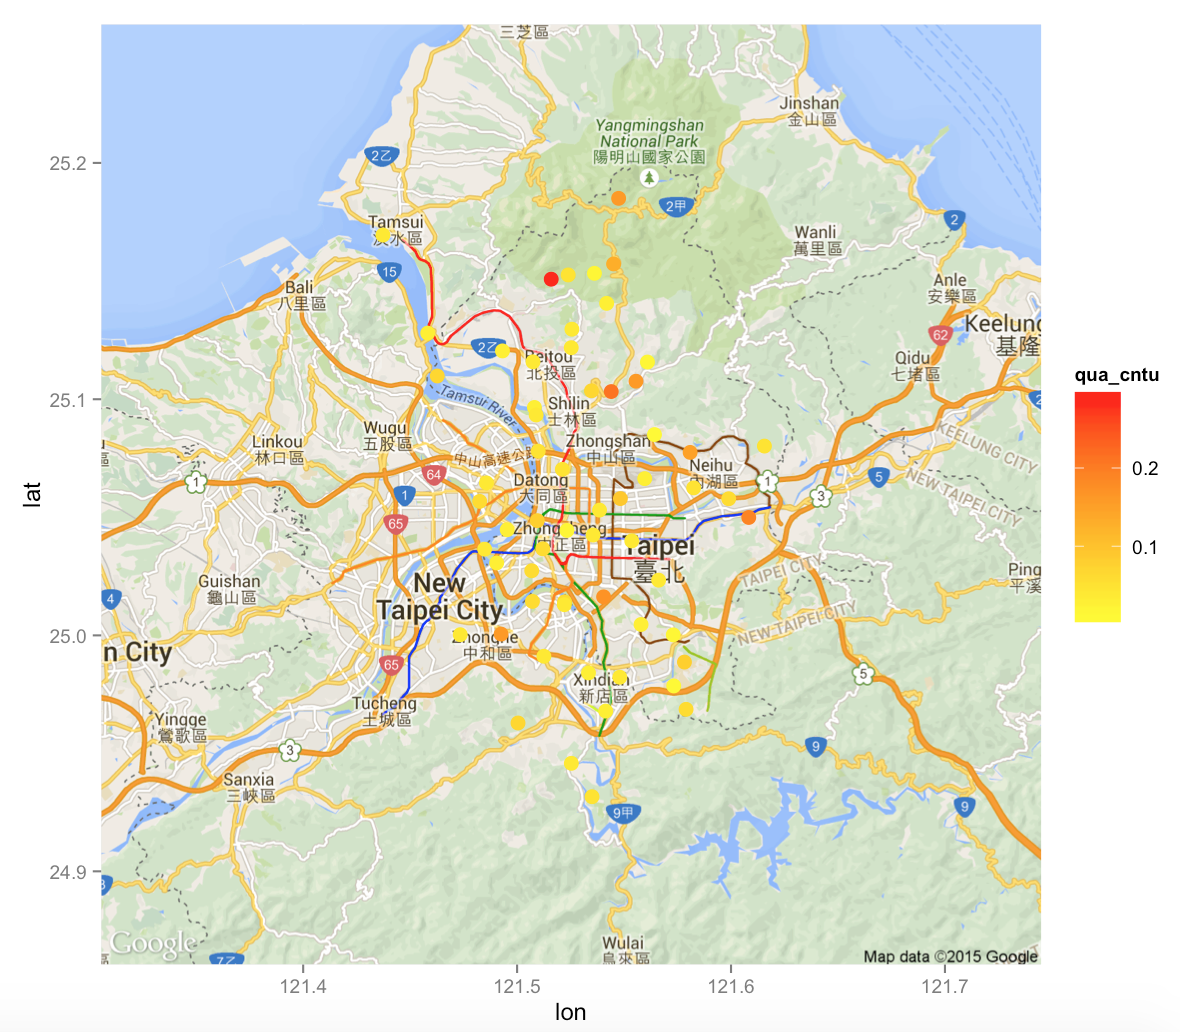
\includegraphics[width=16.39in]{figure/waterQ}

\texttt{ggmap}套件提供多種地圖型態,使用者可透過設定\texttt{maptype}自行選擇適合的地圖樣式,樣式有:

\begin{itemize}
\tightlist
\item
  terrain
\item
  terrain-background
\item
  satellite
\item
  roadmap
\item
  hybrid (google maps)
\item
  watercolor
\item
  toner (stamen maps)
\end{itemize}

透過設定\texttt{extent}參數可將地圖輸出樣式改為滿版

\begin{Shaded}
\begin{Highlighting}[]
\KeywordTok{library}\NormalTok{(ggmap)}
\NormalTok{TaipeiMap =}\StringTok{ }\KeywordTok{get_map}\NormalTok{(}\DataTypeTok{location =} \KeywordTok{c}\NormalTok{(}\FloatTok{121.43}\NormalTok{,}\FloatTok{24.93}\NormalTok{,}\FloatTok{121.62}\NormalTok{,}\FloatTok{25.19}\NormalTok{), }
                    \DataTypeTok{zoom =} \DecValTok{14}\NormalTok{, }\DataTypeTok{maptype =} \StringTok{'roadmap'}\NormalTok{)}
\KeywordTok{ggmap}\NormalTok{(TaipeiMap,}\DataTypeTok{extent =} \StringTok{'device'}\NormalTok{) }\CommentTok{#extent = 'device' 滿版}
\end{Highlighting}
\end{Shaded}

\subsection{Density Map}\label{density-map}

除了面量圖外,密度圖Density
Map也是常用來表示因地理位置不同的數值差異,以下是美國人口密度圖範例
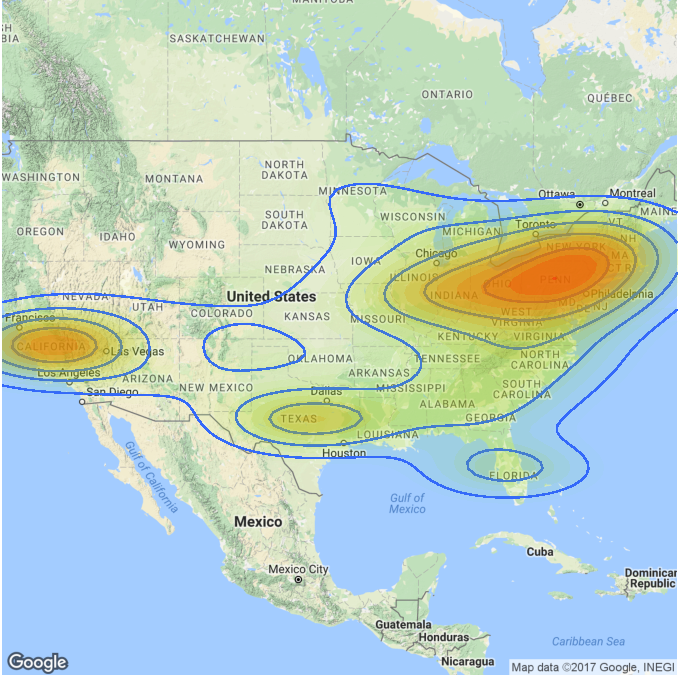
\includegraphics{DataAnalyticsWithR_files/figure-latex/unnamed-chunk-141-1.pdf}

上述範例使用 \texttt{ggplot2} + \texttt{ggmap}
套件來畫人口密度圖,做圖的第一步是資料載入,包括取得美國各州中心座標資料以及美國各州人口資料

\begin{Shaded}
\begin{Highlighting}[]
\CommentTok{#取得美國各州中心座標資料}
\NormalTok{StateCenter<-}\KeywordTok{data.frame}\NormalTok{( }
    \DataTypeTok{region=}\KeywordTok{tolower}\NormalTok{(state.name),}\DataTypeTok{lon=}\NormalTok{state.center$x,}\DataTypeTok{lat=}\NormalTok{state.center$y)}
\KeywordTok{head}\NormalTok{(StateCenter,}\DecValTok{1}\NormalTok{)}
\end{Highlighting}
\end{Shaded}

\begin{verbatim}
##    region lon lat
## 1 alabama -87  33
\end{verbatim}

\begin{Shaded}
\begin{Highlighting}[]
\CommentTok{#美國各州人口資料}
\NormalTok{StatePop<-}\KeywordTok{merge}\NormalTok{(df_pop_state,StateCenter,}\DataTypeTok{by=}\StringTok{"region"}\NormalTok{) }
\KeywordTok{head}\NormalTok{(StatePop,}\DecValTok{1}\NormalTok{)}
\end{Highlighting}
\end{Shaded}

\begin{verbatim}
##    region   value lon lat
## 1 alabama 4777326 -87  33
\end{verbatim}

第二個步驟是將人口數字轉換為\textbf{資料列數},需要這樣轉換的原因是密度圖是用資料列數來決定畫圖的密度,而不是透過單一數值,所以需要在此步驟做轉換

\begin{Shaded}
\begin{Highlighting}[]
\CommentTok{#將人口數值,轉為點!重要!}
\NormalTok{PopPoint<-}\OtherTok{NULL} 
\NormalTok{for(i in }\DecValTok{1}\NormalTok{:}\KeywordTok{nrow}\NormalTok{(StatePop))\{}
    \CommentTok{#每100萬人轉為1點}
    \NormalTok{for(j in }\DecValTok{1}\NormalTok{:(StatePop[i,}\StringTok{"value"}\NormalTok{]/}\DecValTok{1000000}\NormalTok{))\{}
        \NormalTok{PopPoint<-}\KeywordTok{rbind}\NormalTok{(PopPoint,StatePop[i,])   }
    \NormalTok{\}}
\NormalTok{\}}
\KeywordTok{head}\NormalTok{(PopPoint,}\DecValTok{3}\NormalTok{)}
\end{Highlighting}
\end{Shaded}

\begin{verbatim}
##    region   value lon lat
## 1 alabama 4777326 -87  33
## 2 alabama 4777326 -87  33
## 3 alabama 4777326 -87  33
\end{verbatim}

第三個步驟是作圖

\begin{Shaded}
\begin{Highlighting}[]
\NormalTok{USMap <-}\StringTok{ }\KeywordTok{get_map}\NormalTok{(}\DataTypeTok{location =} \StringTok{"United States"}\NormalTok{, }\DataTypeTok{zoom =} \DecValTok{4}\NormalTok{)}
\NormalTok{densityMap<-}\KeywordTok{ggmap}\NormalTok{(USMap, }\DataTypeTok{extent =} \StringTok{"device"}\NormalTok{) +}\StringTok{ }
\StringTok{    }\KeywordTok{geom_density2d}\NormalTok{(}\DataTypeTok{data =} \NormalTok{PopPoint, }\KeywordTok{aes}\NormalTok{(}\DataTypeTok{x =} \NormalTok{lon, }\DataTypeTok{y =} \NormalTok{lat), }\DataTypeTok{size =} \FloatTok{0.3}\NormalTok{) +}\StringTok{ }
\StringTok{    }\KeywordTok{stat_density2d}\NormalTok{(}\DataTypeTok{data =} \NormalTok{PopPoint, }
            \KeywordTok{aes}\NormalTok{(}\DataTypeTok{x =} \NormalTok{lon, }\DataTypeTok{y =} \NormalTok{lat, }\DataTypeTok{fill =} \NormalTok{..level.., }\DataTypeTok{alpha =} \NormalTok{..level..), }
                \DataTypeTok{size =} \FloatTok{0.01}\NormalTok{, }\DataTypeTok{bins =} \DecValTok{16}\NormalTok{, }\DataTypeTok{geom =} \StringTok{"polygon"}\NormalTok{) +}\StringTok{ }
\StringTok{    }\KeywordTok{scale_fill_gradient}\NormalTok{(}\DataTypeTok{low =} \StringTok{"green"}\NormalTok{, }\DataTypeTok{high =} \StringTok{"red"}\NormalTok{, }\DataTypeTok{guide =} \OtherTok{FALSE}\NormalTok{) +}\StringTok{ }
\StringTok{    }\KeywordTok{scale_alpha}\NormalTok{(}\DataTypeTok{range =} \KeywordTok{c}\NormalTok{(}\DecValTok{0}\NormalTok{, }\FloatTok{0.3}\NormalTok{), }\DataTypeTok{guide =} \OtherTok{FALSE}\NormalTok{)}
\NormalTok{densityMap}
\end{Highlighting}
\end{Shaded}

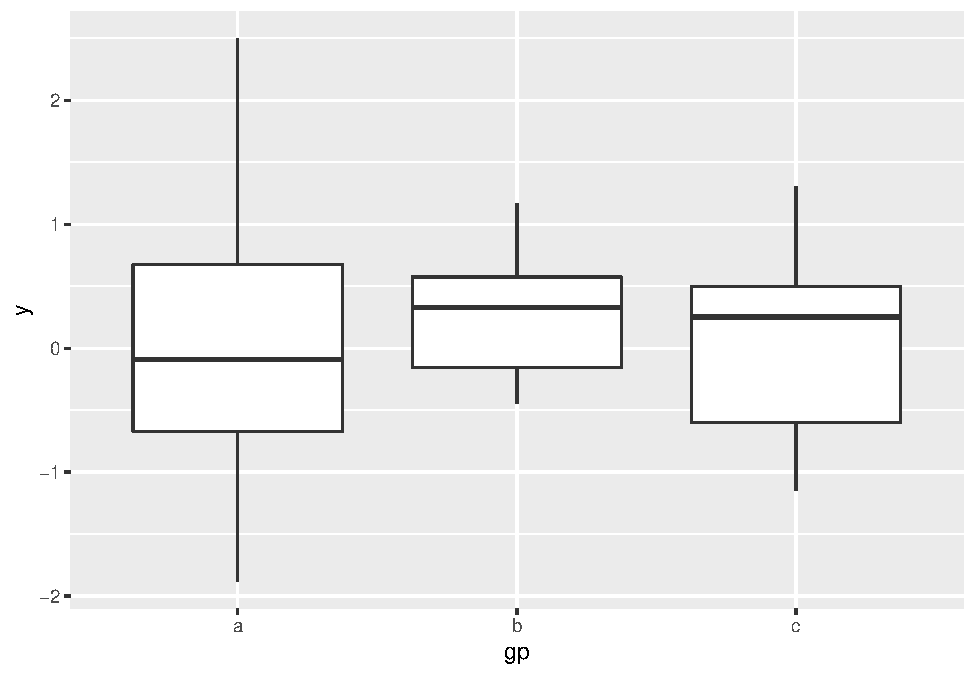
\includegraphics{DataAnalyticsWithR_files/figure-latex/unnamed-chunk-144-1.pdf}

\subsection{參考資料}

\begin{itemize}
\tightlist
\item
  \href{https://github.com/dkahle/ggmap}{ggmap package source code}
\item
  \href{https://www.nceas.ucsb.edu/~frazier/RSpatialGuides/ggmap/ggmapCheatsheet.pdf}{ggmap
  cheat sheet}
\item
  \href{https://dl.dropboxusercontent.com/u/24648660/ggmap\%20useR\%202012.pdf}{ggmap
  doc}
\end{itemize}

\section{Taiwan的面量圖}\label{taiwan}

因為畫台灣的面量圖尚無好的套件輔助,但因Open
Data的關係,我們可以很容易地取得台灣鄉鎮市邊界的經緯度檔案,通常地圖/邊界經緯度檔案是用空間資料開放格式\texttt{shapefile}
\texttt{.shp}儲存,透過\href{http://data.gov.tw/}{政府資料開放平台}可以下載台灣的地圖資料,資料集名稱為\href{http://data.gov.tw/node/7441}{鄉鎮市區界線}。使用\texttt{shapefile}與\texttt{ggplot2}畫圖的步驟如下:

\begin{itemize}
\tightlist
\item
  取得空間資料檔案
\item
  使用\texttt{rgdal}, \texttt{rgeos},\texttt{maptools}
  package處理地圖檔shapefile
\item
  使用\texttt{ggplot2} \& \texttt{RColorBrewer} 畫圖
\end{itemize}

上述套件在第一次使用前需要安裝與載入

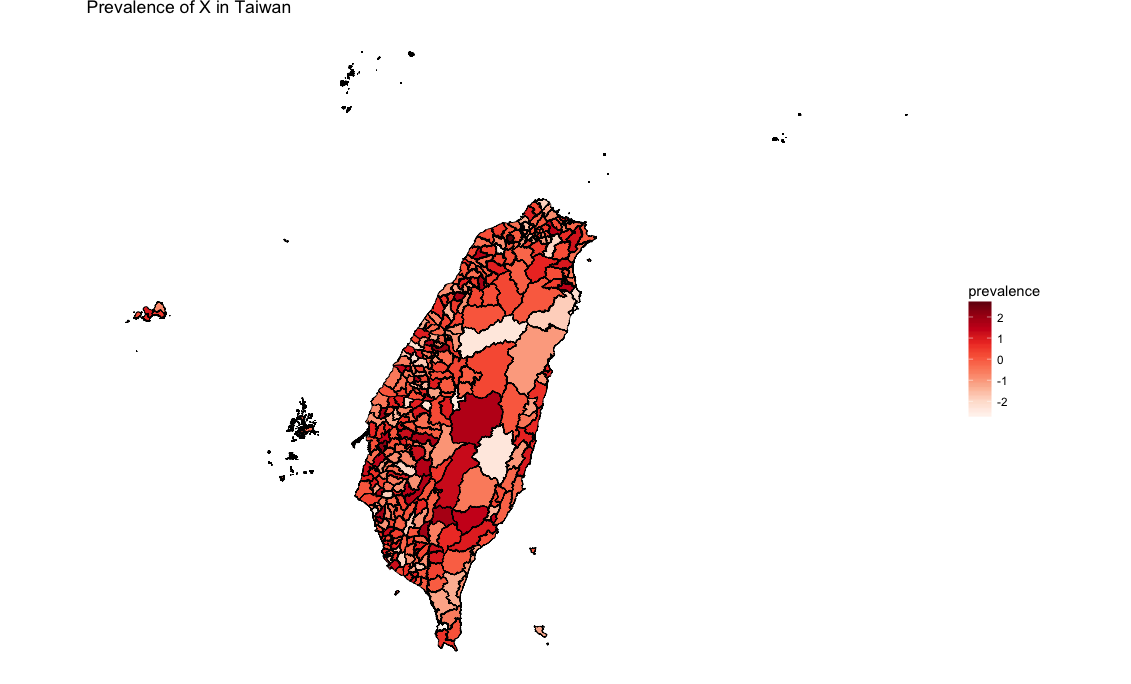
\includegraphics[width=15.71in]{figure/Taiwan}

以上各步驟詳述如下: 1. 處理shapefile-1

\begin{itemize}
\tightlist
\item
  需要\texttt{rgdal}, \texttt{rgeos},\texttt{maptools}
\item
  fortify: 將\texttt{shapefile}物件轉為\texttt{data.frame}
\end{itemize}

\begin{Shaded}
\begin{Highlighting}[]
\KeywordTok{library}\NormalTok{(ggplot2) }\CommentTok{#for fortify(), ggplot(), ggmap()}
\KeywordTok{head}\NormalTok{(tw_new$Town_ID)}
\NormalTok{tw_new.df <-}\StringTok{ }\KeywordTok{fortify}\NormalTok{(tw_new, }\DataTypeTok{region =} \StringTok{"T_UID"}\NormalTok{) }\CommentTok{#from ggplot2 package}
\KeywordTok{head}\NormalTok{(tw_new.df,}\DecValTok{10}\NormalTok{)}
\end{Highlighting}
\end{Shaded}

\begin{verbatim}
       long      lat order  hole piece id group
1  119.9170 26.17518     1 FALSE     1  1   1.1
2  119.9171 26.17517     2 FALSE     1  1   1.1
3  119.9171 26.17518     3 FALSE     1  1   1.1
4  119.9171 26.17518     4 FALSE     1  1   1.1
5  119.9171 26.17518     5 FALSE     1  1   1.1
6  119.9172 26.17518     6 FALSE     1  1   1.1
7  119.9172 26.17518     7 FALSE     1  1   1.1
8  119.9172 26.17518     8 FALSE     1  1   1.1
9  119.9173 26.17515     9 FALSE     1  1   1.1
10 119.9173 26.17515    10 FALSE     1  1   1.1
\end{verbatim}

\begin{enumerate}
\def\labelenumi{\arabic{enumi}.}
\setcounter{enumi}{1}
\tightlist
\item
  做一個假資料來畫:著色基準檔
\end{enumerate}

\begin{Shaded}
\begin{Highlighting}[]
\CommentTok{#做一個假資料來畫}
\CommentTok{#prevalence設為亂數rnorm(需要的亂數個數)}
\NormalTok{mydata<-}\KeywordTok{data.frame}\NormalTok{(}\DataTypeTok{NAME_2=}\NormalTok{tw_new$T_Name, }\DataTypeTok{id=}\NormalTok{tw_new$T_UID,}
                   \DataTypeTok{prevalence=}\KeywordTok{rnorm}\NormalTok{(}\KeywordTok{length}\NormalTok{(tw_new$T_UID)))}
\KeywordTok{head}\NormalTok{(mydata)}
\end{Highlighting}
\end{Shaded}

\begin{verbatim}
                  NAME_2  id prevalence
1 \xa6\xa8\xa5\\\xc2\xed 178  1.0551637
2            \xa8ΥV\xb6m 164 -0.6307466
3     \xb3\xc1\xbcd\xb6m 118 -1.2255327
4     \xba\xf1\xaeq\xb6m 376  0.1314583
5  \xc4\xf5\xc0\xac\xb6m 369  1.3665832
6      \xa5Ф\xa4\xc2\xed  78 -0.3132549
\end{verbatim}

\begin{enumerate}
\def\labelenumi{\arabic{enumi}.}
\setcounter{enumi}{2}
\tightlist
\item
  處理中文編碼
  利用iconv將不知所以然的代碼(\xa6\xa8\xa5\textbackslash{}\xc2\xed)轉為看得懂的中文
\end{enumerate}

\begin{Shaded}
\begin{Highlighting}[]
\CommentTok{#from big5 to utf-8}
\NormalTok{mydata$NAME_2<-}\KeywordTok{iconv}\NormalTok{(}\KeywordTok{as.character}\NormalTok{(mydata$NAME_2), }\CommentTok{#NAME_2原本是factor}
                     \DataTypeTok{from=}\StringTok{"big5"}\NormalTok{, }\DataTypeTok{to =} \StringTok{"UTF-8"}\NormalTok{)}
\KeywordTok{head}\NormalTok{(mydata,}\DecValTok{10}\NormalTok{)}
\end{Highlighting}
\end{Shaded}

\begin{verbatim}
   NAME_2  id prevalence
1  成功鎮 178  1.0551637
2  佳冬鄉 164 -0.6307466
3  麥寮鄉 118 -1.2255327
4  綠島鄉 376  0.1314583
5  蘭嶼鄉 369  1.3665832
6  田中鎮  78 -0.3132549
7  社頭鄉  83  1.2072224
8  竹田鄉 157  0.7312959
9  萬丹鄉 148  1.4849184
10 三灣鄉  64  0.6094254
\end{verbatim}

\begin{enumerate}
\def\labelenumi{\arabic{enumi}.}
\setcounter{enumi}{3}
\tightlist
\item
  合併的圖檔與著色基準檔
  最後將有prevalence的假數據mydata和經緯度資料tw\_new.df合併, 用merge()
\end{enumerate}

\begin{Shaded}
\begin{Highlighting}[]
\NormalTok{final.plot<-}\KeywordTok{merge}\NormalTok{(tw_new.df,mydata,}\DataTypeTok{by=}\StringTok{"id"}\NormalTok{,}\DataTypeTok{all.x=}\NormalTok{T)}
\KeywordTok{head}\NormalTok{(final.plot,}\DecValTok{10}\NormalTok{)}
\end{Highlighting}
\end{Shaded}

\begin{verbatim}
   id     long      lat order  hole piece group NAME_2 prevalence
1   1 119.9170 26.17518     1 FALSE     1   1.1 南竿鄉  0.9584632
2   1 119.9171 26.17517     2 FALSE     1   1.1 南竿鄉  0.9584632
3   1 119.9171 26.17518     3 FALSE     1   1.1 南竿鄉  0.9584632
4   1 119.9171 26.17518     4 FALSE     1   1.1 南竿鄉  0.9584632
5   1 119.9171 26.17518     5 FALSE     1   1.1 南竿鄉  0.9584632
6   1 119.9172 26.17518     6 FALSE     1   1.1 南竿鄉  0.9584632
7   1 119.9172 26.17518     7 FALSE     1   1.1 南竿鄉  0.9584632
8   1 119.9172 26.17518     8 FALSE     1   1.1 南竿鄉  0.9584632
9   1 119.9173 26.17515     9 FALSE     1   1.1 南竿鄉  0.9584632
10  1 119.9173 26.17515    10 FALSE     1   1.1 南竿鄉  0.9584632
\end{verbatim}

\begin{enumerate}
\def\labelenumi{\arabic{enumi}.}
\setcounter{enumi}{4}
\tightlist
\item
  畫台灣面量圖
\end{enumerate}

\begin{Shaded}
\begin{Highlighting}[]
\KeywordTok{library}\NormalTok{(RColorBrewer) }\CommentTok{#配色用brewer.pal( 9 , "Reds" )}
\NormalTok{twcmap<-}\KeywordTok{ggplot}\NormalTok{() +}
\StringTok{    }\KeywordTok{geom_polygon}\NormalTok{(}\DataTypeTok{data =} \NormalTok{final.plot, }
                 \KeywordTok{aes}\NormalTok{(}\DataTypeTok{x =} \NormalTok{long, }\DataTypeTok{y =} \NormalTok{lat, }\DataTypeTok{group =} \NormalTok{group, }
                     \DataTypeTok{fill =} \NormalTok{prevalence), }
                 \DataTypeTok{color =} \StringTok{"black"}\NormalTok{, }\DataTypeTok{size =} \FloatTok{0.25}\NormalTok{) +}\StringTok{ }
\StringTok{    }\KeywordTok{coord_map}\NormalTok{()+}\CommentTok{#維持地圖比例}
\StringTok{    }\KeywordTok{scale_fill_gradientn}\NormalTok{(}\DataTypeTok{colours =} \KeywordTok{brewer.pal}\NormalTok{(}\DecValTok{9}\NormalTok{,}\StringTok{"Reds"}\NormalTok{))+}
\StringTok{    }\KeywordTok{theme_void}\NormalTok{()+}
\StringTok{    }\KeywordTok{labs}\NormalTok{(}\DataTypeTok{title=}\StringTok{"Prevalence of X in Taiwan"}\NormalTok{)}
\NormalTok{twcmap}
\end{Highlighting}
\end{Shaded}

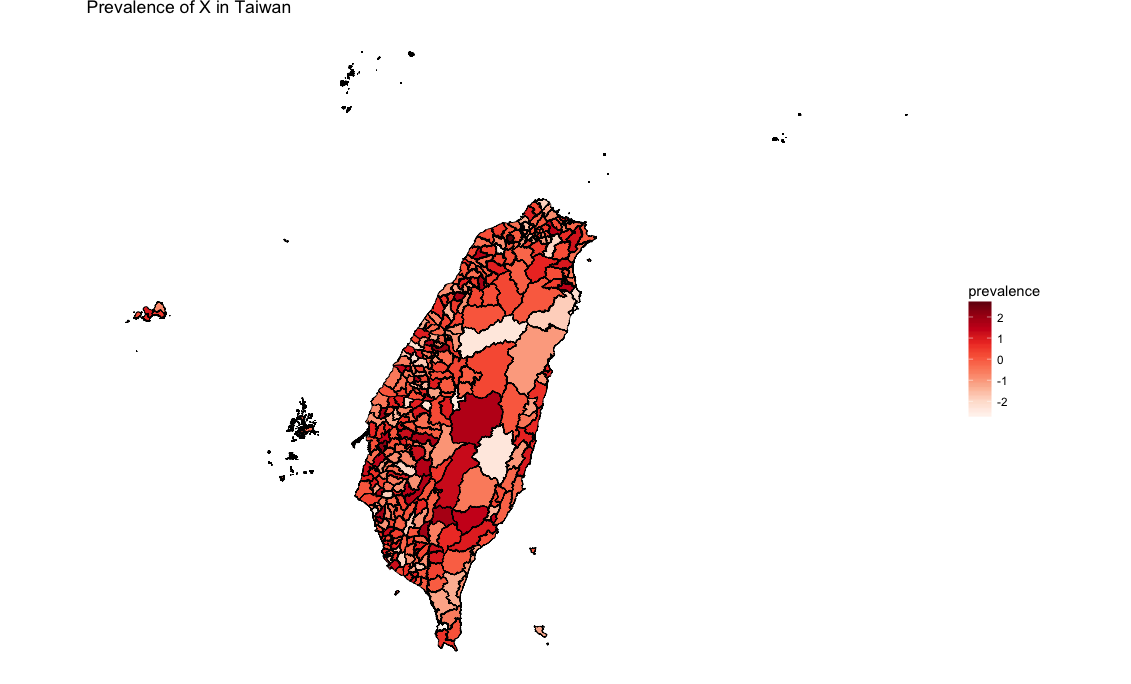
\includegraphics[width=15.71in]{figure/Taiwan}

\subsection{ggmap+面量圖}\label{ggmap}

\begin{Shaded}
\begin{Highlighting}[]
\KeywordTok{library}\NormalTok{(ggmap)}
\NormalTok{twmap <-}\StringTok{ }\KeywordTok{get_map}\NormalTok{(}\DataTypeTok{location =} \StringTok{'Taiwan'}\NormalTok{, }\DataTypeTok{zoom =} \DecValTok{7}\NormalTok{,}\DataTypeTok{language =} \StringTok{"zh-TW"}\NormalTok{)}
\KeywordTok{ggmap}\NormalTok{(twmap)+}\StringTok{ }\CommentTok{#ggmap}
\StringTok{    }\KeywordTok{geom_polygon}\NormalTok{(}\DataTypeTok{data =} \NormalTok{final.plot,  }\CommentTok{#面量圖}
        \KeywordTok{aes}\NormalTok{(}\DataTypeTok{x =} \NormalTok{long, }\DataTypeTok{y =} \NormalTok{lat, }\DataTypeTok{group =} \NormalTok{group, }\DataTypeTok{fill =} \NormalTok{prevalence), }
        \DataTypeTok{color =} \StringTok{"grey80"}\NormalTok{, }\DataTypeTok{size =} \FloatTok{0.1}\NormalTok{,}\DataTypeTok{alpha =} \FloatTok{0.5}\NormalTok{) +}\StringTok{ }
\KeywordTok{scale_fill_gradientn}\NormalTok{(}\DataTypeTok{colours =} \KeywordTok{brewer.pal}\NormalTok{(}\DecValTok{9}\NormalTok{,}\StringTok{"Reds"}\NormalTok{))}
\end{Highlighting}
\end{Shaded}

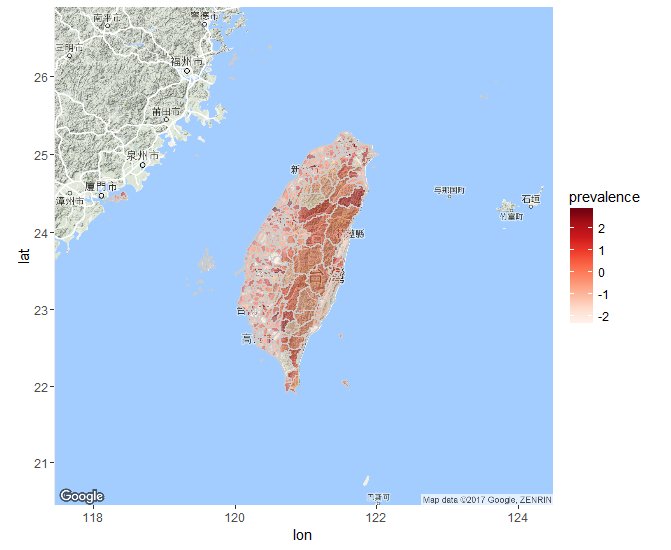
\includegraphics[width=9.32in]{figure/ggmapTaiwan}

\section{Heatmap}\label{heatmap}

\texttt{Heatmap}熱度圖使用顏色的深淺來表示數值的大小,通常會搭配XY兩軸的變量,所以使用一張圖就能表示三個維度的資訊,在ggplot2套件中,可以使用\texttt{geom\_tile()}來畫Heatmap,以下以NBA球員的資料作為範例,希望能透過Heatmap來呈現球員表現的差異。
首先先將檔案讀入

\begin{Shaded}
\begin{Highlighting}[]
\CommentTok{#讀.csv檔案}
\NormalTok{nba <-}\StringTok{ }\KeywordTok{read.csv}\NormalTok{(}\StringTok{"http://datasets.flowingdata.com/ppg2008.csv"}\NormalTok{)}
\KeywordTok{head}\NormalTok{(nba)}
\end{Highlighting}
\end{Shaded}

\begin{verbatim}
##             Name  G MIN PTS  FGM FGA  FGP FTM FTA  FTP X3PM X3PA X3PP ORB DRB
## 1   Dwyane Wade  79  39  30 10.8  22 0.49 7.5 9.8 0.77  1.1  3.5 0.32 1.1 3.9
## 2  LeBron James  81  38  28  9.7  20 0.49 7.3 9.4 0.78  1.6  4.7 0.34 1.3 6.3
## 3   Kobe Bryant  82  36  27  9.8  21 0.47 5.9 6.9 0.86  1.4  4.1 0.35 1.1 4.1
## 4 Dirk Nowitzki  81  38  26  9.6  20 0.48 6.0 6.7 0.89  0.8  2.1 0.36 1.1 7.3
## 5 Danny Granger  67  36  26  8.5  19 0.45 6.0 6.9 0.88  2.7  6.7 0.40 0.7 4.4
## 6  Kevin Durant  74  39  25  8.9  19 0.48 6.1 7.1 0.86  1.3  3.1 0.42 1.0 5.5
##   TRB AST STL BLK  TO  PF
## 1 5.0 7.5 2.2 1.3 3.4 2.3
## 2 7.6 7.2 1.7 1.1 3.0 1.7
## 3 5.2 4.9 1.5 0.5 2.6 2.3
## 4 8.4 2.4 0.8 0.8 1.9 2.2
## 5 5.1 2.7 1.0 1.4 2.5 3.1
## 6 6.5 2.8 1.3 0.7 3.0 1.8
\end{verbatim}

為了做圖,將寬表轉長表,寬表與長表的概念可參見\ref{reshape}

\begin{Shaded}
\begin{Highlighting}[]
\KeywordTok{library}\NormalTok{(reshape2) }\CommentTok{#for melt()}
\NormalTok{nba.m <-}\StringTok{ }\KeywordTok{melt}\NormalTok{(nba,}\DataTypeTok{id.vars =} \StringTok{"Name"}\NormalTok{) }\CommentTok{#寬表轉長表,以名字作依據}
\KeywordTok{head}\NormalTok{(nba.m,}\DecValTok{10}\NormalTok{)}
\end{Highlighting}
\end{Shaded}

\begin{verbatim}
##                Name variable value
## 1      Dwyane Wade         G    79
## 2     LeBron James         G    81
## 3      Kobe Bryant         G    82
## 4    Dirk Nowitzki         G    81
## 5    Danny Granger         G    67
## 6     Kevin Durant         G    74
## 7     Kevin Martin         G    51
## 8     Al Jefferson         G    50
## 9       Chris Paul         G    78
## 10 Carmelo Anthony         G    66
\end{verbatim}

將Geometric objects指定為\texttt{geom\_tile()},完成Heatmap

\begin{Shaded}
\begin{Highlighting}[]
\KeywordTok{library}\NormalTok{(ggplot2) }\CommentTok{#for ggplot()}
\KeywordTok{ggplot}\NormalTok{(nba.m, }\KeywordTok{aes}\NormalTok{(variable, Name)) +}\StringTok{ }\CommentTok{#aes(x,y)}
\StringTok{    }\KeywordTok{geom_tile}\NormalTok{(}\KeywordTok{aes}\NormalTok{(}\DataTypeTok{fill =} \NormalTok{value),}\DataTypeTok{colour =} \StringTok{"white"}\NormalTok{)+}\StringTok{ }\CommentTok{#geom_tile: 區塊著色}
\StringTok{    }\KeywordTok{scale_fill_gradient}\NormalTok{(}\DataTypeTok{low =} \StringTok{"white"}\NormalTok{,}\DataTypeTok{high =} \StringTok{"steelblue"}\NormalTok{) }\CommentTok{#數值低:白色}
\end{Highlighting}
\end{Shaded}

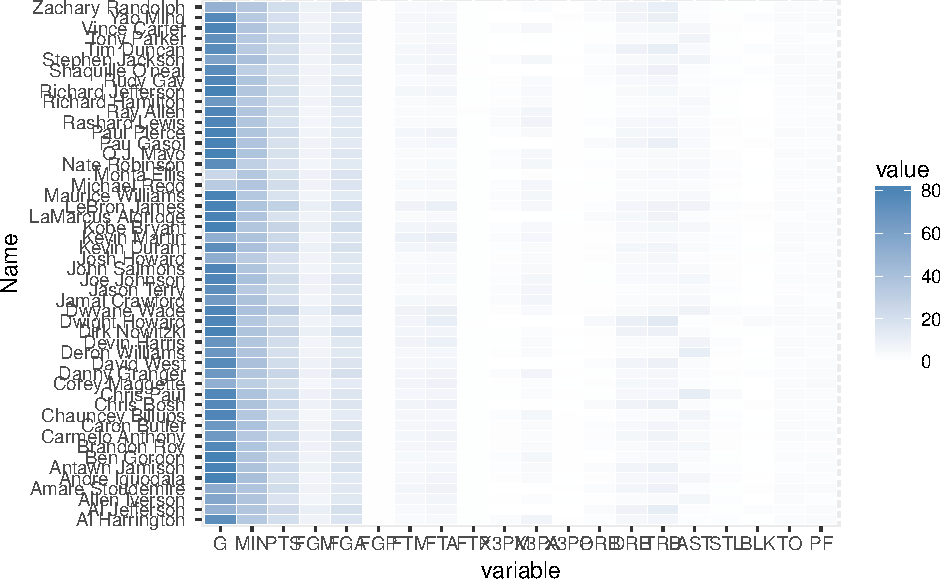
\includegraphics{DataAnalyticsWithR_files/figure-latex/unnamed-chunk-157-1.pdf}

看上圖可以發現,因為G欄資料明顯大於其他欄位,導致顏色差異不明顯,為了解決此問題,將個欄位的資料標準化處理,這邊使用到apply函式

apply()有類似for迴圈的功能

\begin{itemize}
\tightlist
\item
  apply(Data, MARGIN, FUN,\ldots{})

  \begin{itemize}
  \tightlist
  \item
    Data:矩陣(Matrix),Data Frame
  \item
    MARGIN:1=row, 2=column
  \item
    FUN:函數
  \item
    \ldots{}:函數要用的參數
  \end{itemize}
\end{itemize}

\begin{Shaded}
\begin{Highlighting}[]
\NormalTok{nba[,}\DecValTok{2}\NormalTok{:}\DecValTok{21}\NormalTok{]<-}\KeywordTok{apply}\NormalTok{(nba[,}\DecValTok{2}\NormalTok{:}\DecValTok{21}\NormalTok{], }\DecValTok{2}\NormalTok{, scale) }\CommentTok{#scale處理,將數值轉為平均=0}
\KeywordTok{head}\NormalTok{(nba,}\DecValTok{2}\NormalTok{)}
\end{Highlighting}
\end{Shaded}

\begin{verbatim}
##            Name    G  MIN PTS FGM FGA  FGP FTM FTA   FTP  X3PM X3PA   X3PP
## 1  Dwyane Wade  0.62 1.00 3.2 2.9 2.6 0.51 1.9 2.1 -0.74 -0.11 0.13 -0.157
## 2 LeBron James  0.77 0.61 2.6 2.0 1.7 0.46 1.8 1.9 -0.52  0.49 0.70  0.027
##      ORB   DRB   TRB AST STL  BLK  TO   PF
## 1 -0.272 -0.35 -0.33 1.7 2.6 1.21 1.8 -0.3
## 2 -0.061  1.01  0.66 1.5 1.4 0.86 1.1 -1.4
\end{verbatim}

\begin{Shaded}
\begin{Highlighting}[]
\NormalTok{nba.m <-}\StringTok{ }\KeywordTok{melt}\NormalTok{(nba) ##寬轉長}
\KeywordTok{ggplot}\NormalTok{(nba.m, }\KeywordTok{aes}\NormalTok{(variable, Name)) +}\StringTok{ }
\StringTok{    }\KeywordTok{geom_tile}\NormalTok{(}\KeywordTok{aes}\NormalTok{(}\DataTypeTok{fill =} \NormalTok{value),}\DataTypeTok{colour =} \StringTok{"white"}\NormalTok{)+}\StringTok{ }\CommentTok{#geom_tile: 區塊著色}
\StringTok{    }\KeywordTok{scale_fill_gradient}\NormalTok{(}\DataTypeTok{low =} \StringTok{"white"}\NormalTok{,}\DataTypeTok{high =} \StringTok{"steelblue"}\NormalTok{) }\CommentTok{#數值低:白色}
\end{Highlighting}
\end{Shaded}

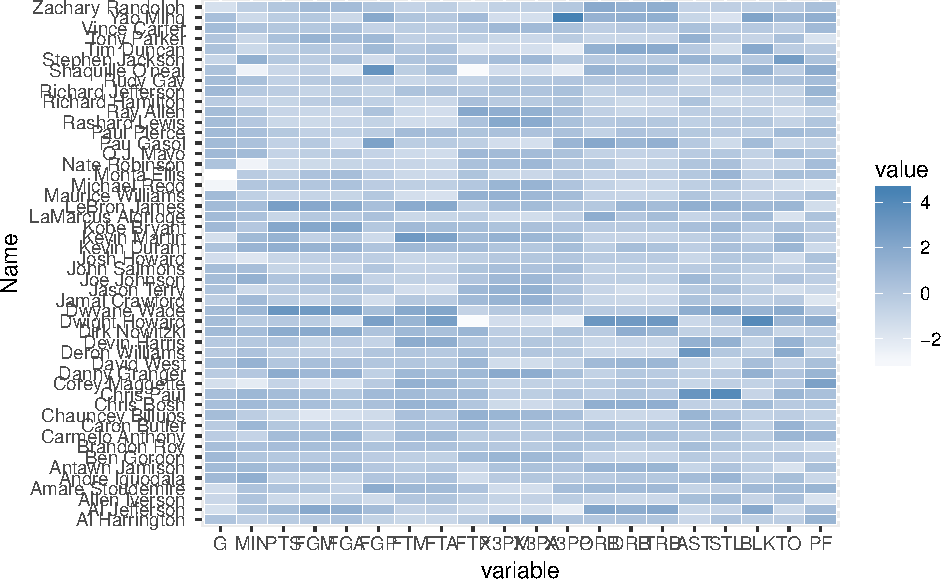
\includegraphics{DataAnalyticsWithR_files/figure-latex/unnamed-chunk-158-1.pdf}

以上範例之參考資料為\href{http://flowingdata.com/2010/01/21/how-to-make-a-heatmap-a-quick-and-easy-solution/}{How
to Make a Heatmap -- a Quick and Easy Solution}

\section{Treemap}\label{treemap}

Treemap(矩形式樹狀結構繪圖法)是以二維平面的方式展示包含階層結構(hierarchical)形式的統計資訊,在R中可以使用\texttt{treemapify}\citep{R-treemapify}
packages

\begin{Shaded}
\begin{Highlighting}[]
\KeywordTok{install.packages}\NormalTok{(}\StringTok{"devtools"}\NormalTok{)}
\KeywordTok{library}\NormalTok{(devtools)}
\KeywordTok{install_github}\NormalTok{(}\StringTok{"wilkox/ggfittext"}\NormalTok{)}
\KeywordTok{install_github}\NormalTok{(}\StringTok{"wilkox/treemapify"}\NormalTok{) }
\end{Highlighting}
\end{Shaded}

\begin{Shaded}
\begin{Highlighting}[]
\KeywordTok{library}\NormalTok{(treemapify)}
\end{Highlighting}
\end{Shaded}

以G20 Dataset為例,二十國集團(英語:Group of
Twenty,縮寫:G20)是一個國際經濟合作論壇,於1999年12月16日在德國柏林成立,屬於布雷頓森林體系框架內非正式對話的一種機制,由七國集團(美國、英國、法國、德國、義大利、日本、加拿大),金磚五國(中國、印度、巴西、俄羅斯、南非),七個重要經濟體(澳大利亞、墨西哥、韓國、土耳其、印尼、沙烏地阿拉伯、阿根廷),以及歐盟組成。按照慣例,國際貨幣基金組織與世界銀行列席該組織的會議。二十國集團的GDP總量約佔全球GDP的85%,貿易佔全球貿易總額的80\%以上,人口約佔全球人口的2/3。(\href{https://en.wikipedia.org/wiki/G-20_major_economies}{維基百科})

G20 Dataset包含20個國家的資訊,資料欄位有:

\begin{itemize}
\tightlist
\item
  Region 國家所在區域
\item
  Country 國家名稱
\item
  Trade.mil.USD 總貿易額,以百萬為單位
\item
  Nom.GDP.mil.USD 名義國內生產總值,以百萬為單位
\item
  HDI
  人類發展指數(\href{https://zh.wikipedia.org/zh-tw/\%E4\%BA\%BA\%E7\%B1\%BB\%E5\%8F\%91\%E5\%B1\%95\%E6\%8C\%87\%E6\%95\%B0}{維基百科})
\item
  Population 人口數
\item
  Economic.classification 經濟狀況分類
\end{itemize}

首先將資料讀入,並用\texttt{str()}函式觀察資料型態

\begin{Shaded}
\begin{Highlighting}[]
\KeywordTok{data}\NormalTok{(G20)}\CommentTok{#範例資料}
\KeywordTok{str}\NormalTok{(G20)}
\end{Highlighting}
\end{Shaded}

\begin{verbatim}
## 'data.frame':    20 obs. of  7 variables:
##  $ Region                 : Factor w/ 8 levels "Africa","Asia",..: 1 6 6 6 8 8 2 2 2 2 ...
##  $ Country                : Factor w/ 20 levels " Argentina"," Australia",..: 15 19 4 12 3 1 5 11 16 8 ...
##  $ Trade.mil.USD          : int  208000 3969000 962600 756800 494800 152690 3801000 1649800 1068700 809400 ...
##  $ Nom.GDP.mil.USD        : int  384315 15684750 1819081 1177116 2395968 474954 8227037 5963969 1155872 1824832 ...
##  $ HDI                    : num  0.629 0.937 0.911 0.775 0.73 0.811 0.699 0.912 0.909 0.554 ...
##  $ Population             : int  53000000 316173000 34088000 112211789 201032714 40117096 1339724852 127390000 50004441 1210193422 ...
##  $ Economic.classification: Factor w/ 2 levels "Advanced","Developing": 2 1 1 2 2 2 2 1 1 2 ...
\end{verbatim}

畫Treemap的第一個步驟是用\texttt{treemapify()}函式將資料轉為畫Treemap所需格式,此格式要包括下列欄位:

\begin{itemize}
\tightlist
\item
  area: 面積來源(GDP)
\item
  fill: 著色來源(HDI)
\item
  label: 每個方塊分類依據(Country)
\item
  group: 方塊群組(Region)
\end{itemize}

\begin{Shaded}
\begin{Highlighting}[]
\NormalTok{treeMapCoordinates <-}\StringTok{ }\KeywordTok{treemapify}\NormalTok{(}\DataTypeTok{data=}\NormalTok{G20, }\CommentTok{#data=資料來源(G20)}
    \DataTypeTok{area =} \StringTok{"Nom.GDP.mil.USD"}\NormalTok{,}\DataTypeTok{fill =} \StringTok{"HDI"}\NormalTok{, }\CommentTok{#面積依GDP,顏色用HDI}
    \DataTypeTok{label =} \StringTok{"Country"}\NormalTok{,}\DataTypeTok{group =} \StringTok{"Region"}\NormalTok{) }\CommentTok{#方塊分類依據用國家,再用地區分群}
\KeywordTok{head}\NormalTok{(treeMapCoordinates)}
\end{Highlighting}
\end{Shaded}

\begin{verbatim}
##   fill           label xmin xmax ymin ymax         group
## 1 0.88  European Union    0   39    0   59        Europe
## 2 0.92         Germany   39   63    0   19        Europe
## 3 0.89          France   39   63   19   34        Europe
## 4 0.88  United Kingdom   39   63   34   48        Europe
## 5 0.88           Italy   39   63   48   59        Europe
## 6 0.94   United States    0   53   59  100 North America
\end{verbatim}

用\texttt{treemapify()}完成資料轉換後,使用\texttt{ggplotify()}函式做圖

\begin{Shaded}
\begin{Highlighting}[]
\KeywordTok{ggplotify}\NormalTok{(treeMapCoordinates)}
\end{Highlighting}
\end{Shaded}

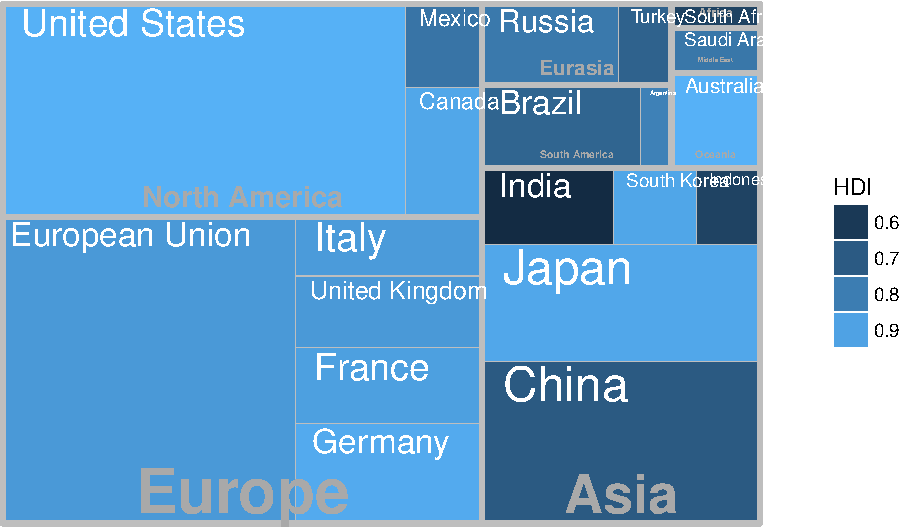
\includegraphics{DataAnalyticsWithR_files/figure-latex/ggplotify1-1.pdf}

看函式名稱不難了解\texttt{ggplotify()}也是基於\texttt{ggplot2}套件開發,所以可以使用ggplot2的圖形設定參數改變圖形樣式,由於數字越大顏色越深比較符合視覺化的常理,所以這邊使用\texttt{ggplot2}的\texttt{scale\_fill\_gradient()}函式指定數值高低所需的顏色

\begin{Shaded}
\begin{Highlighting}[]
\KeywordTok{ggplotify}\NormalTok{(treeMapCoordinates)+}\StringTok{ }
\StringTok{    }\KeywordTok{scale_fill_gradient}\NormalTok{(}\DataTypeTok{low =} \StringTok{"white"}\NormalTok{,}\DataTypeTok{high =} \StringTok{"steelblue"}\NormalTok{) }\CommentTok{#指定高低顏色}
\end{Highlighting}
\end{Shaded}

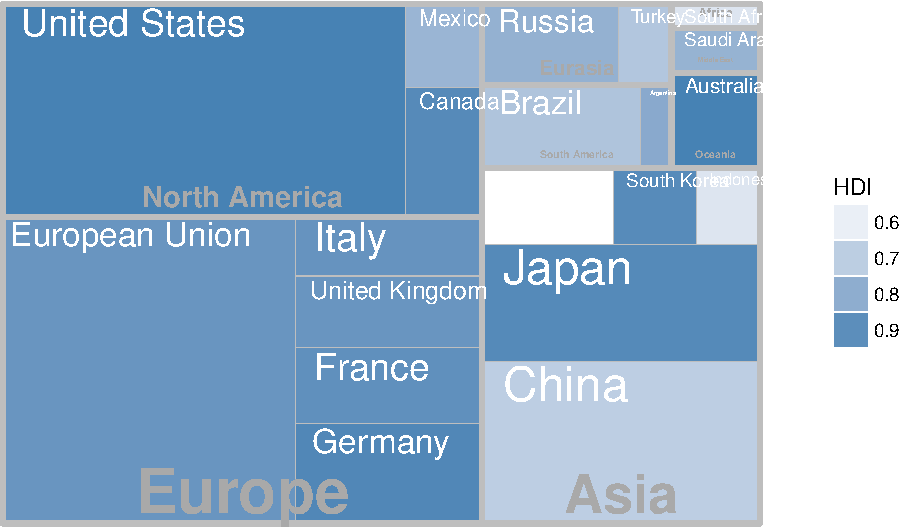
\includegraphics{DataAnalyticsWithR_files/figure-latex/ggplotify2-1.pdf}

完整做圖程式碼如下:

\begin{Shaded}
\begin{Highlighting}[]
\NormalTok{## install.packages("devtools") 第一次使用前需要安裝}
\NormalTok{## library(devtools)}
\NormalTok{## install_github("wilkox/treemapify") }
\KeywordTok{library}\NormalTok{(treemapify)}
\KeywordTok{data}\NormalTok{(G20)}\CommentTok{#載入範例資料}
\NormalTok{treeMapCoordinates <-}\StringTok{ }\KeywordTok{treemapify}\NormalTok{(}\DataTypeTok{data=}\NormalTok{G20, }\CommentTok{#data=資料來源(G20)}
    \DataTypeTok{area =} \StringTok{"Nom.GDP.mil.USD"}\NormalTok{,}\DataTypeTok{fill =} \StringTok{"HDI"}\NormalTok{,}
    \DataTypeTok{label =} \StringTok{"Country"}\NormalTok{,}\DataTypeTok{group =} \StringTok{"Region"}\NormalTok{)}
\KeywordTok{ggplotify}\NormalTok{(treeMapCoordinates)+}\StringTok{ }
\StringTok{    }\KeywordTok{scale_fill_gradient}\NormalTok{(}\DataTypeTok{low =} \StringTok{"white"}\NormalTok{,}\DataTypeTok{high =} \StringTok{"steelblue"}\NormalTok{) }\CommentTok{#指定高低顏色}
\end{Highlighting}
\end{Shaded}

\texttt{treemap}\citep{R-treemap} package也提供相同的功能

\begin{Shaded}
\begin{Highlighting}[]
\KeywordTok{library}\NormalTok{(treemap)}
\KeywordTok{data}\NormalTok{(GNI2014)}
\KeywordTok{treemap}\NormalTok{(GNI2014,}
       \DataTypeTok{index=}\KeywordTok{c}\NormalTok{(}\StringTok{"continent"}\NormalTok{, }\StringTok{"iso3"}\NormalTok{),}
       \DataTypeTok{vSize=}\StringTok{"population"}\NormalTok{,}
       \DataTypeTok{vColor=}\StringTok{"GNI"}\NormalTok{,}
       \DataTypeTok{type=}\StringTok{"value"}\NormalTok{)}
\end{Highlighting}
\end{Shaded}

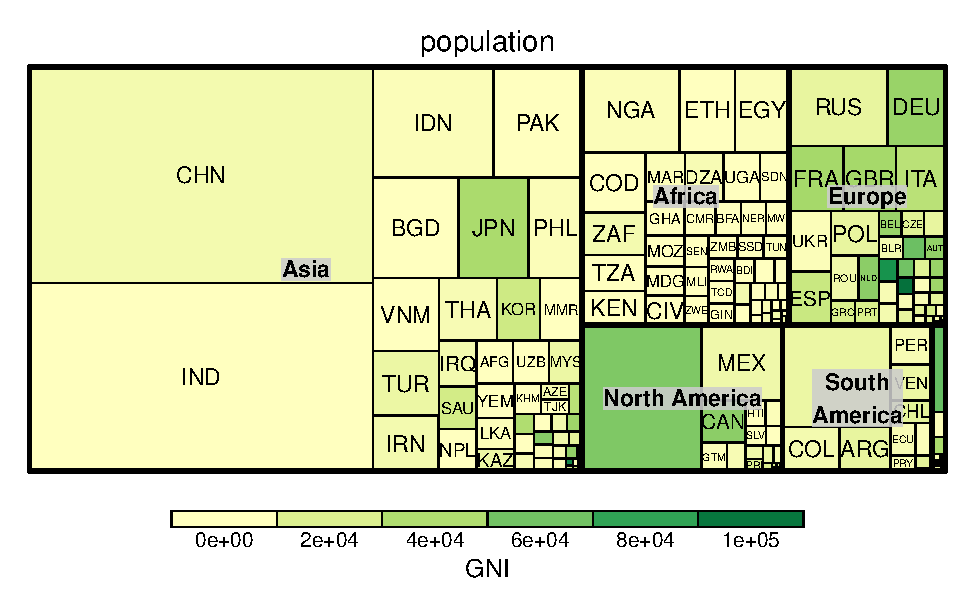
\includegraphics{DataAnalyticsWithR_files/figure-latex/treemap1-1.pdf}

\href{https://github.com/wilkox/treemapify}{參考資料}

\section{參考文件與資源}\label{-2}

\begin{itemize}
\tightlist
\item
  官方網站\href{http://docs.ggplot2.org/current/}{文件}
\item
  RStudio製作的\href{https://www.rstudio.com/wp-content/uploads/2016/11/ggplot2-cheatsheet-2.1.pdf}{ggplot
  cheat sheet}
\item
  DataCamp互動式課程1
  \href{https://www.datacamp.com/courses/data-visualization-with-ggplot2-1}{Data
  Visualization with ggplot2 (Part 1)}
\item
  DataCamp互動式課程2
  \href{https://www.datacamp.com/courses/data-visualization-with-ggplot2-2}{Data
  Visualization with ggplot2 (Part 2)}
\item
  DataCamp互動式課程3
  \href{https://www.datacamp.com/courses/data-visualization-with-ggplot2-3}{Data
  Visualization with ggplot2 (Part 3)}
\end{itemize}

\chapter{互動式資料呈現}\label{InteractiveGraphics}

在R中有多種互動式資料呈現方式,除了傳統的\texttt{GGobi}、\texttt{iPlots}、\texttt{identify}等套件外,結合網頁呈現的互動畫呈現方式有更多的彈性,以下介紹幾種好用的互動式套件:

\begin{itemize}
\tightlist
\item
  ggvis
\item
  googleVis
\item
  Plot.ly
\end{itemize}

使用者可依需求選擇使用。

最後再介紹Shiny,一個RStudio推出供R語言使用的網頁應用框架,使用者可以將做好的互動式圖表用Shiny部署網頁,並將分析結果以網頁的方式分享給別人。

\section{ggvis}\label{ggvis}

ggvis\citep{R-ggvis}
是RStudio開發的互動式繪圖套件,繪圖語法與ggplot2\citep{R-ggplot2}套件類似,基本概念是使用R做資料處理與分析,然後利用網頁的方式做視覺化呈現。如果使用RStudio
IDE,透過ggvis套件畫的圖會呈現在右下角的\textbf{Viewer}視窗中。

使用ggvis套件時,必須先安裝與載入

\begin{Shaded}
\begin{Highlighting}[]
\KeywordTok{install.packages}\NormalTok{(}\StringTok{"ggvis"}\NormalTok{)}
\end{Highlighting}
\end{Shaded}

\begin{Shaded}
\begin{Highlighting}[]
\KeywordTok{library}\NormalTok{(ggvis)}
\end{Highlighting}
\end{Shaded}

\begin{Shaded}
\begin{Highlighting}[]
\NormalTok{p <-}\StringTok{ }\KeywordTok{ggvis}\NormalTok{(mtcars, }\DataTypeTok{x =} \NormalTok{~wt, }\DataTypeTok{y =} \NormalTok{~mpg)}
\KeywordTok{layer_points}\NormalTok{(p)}
\end{Highlighting}
\end{Shaded}

\hypertarget{plot_id578777234-container}{}
\hypertarget{plot_id578777234}{}

Renderer: SVG \textbar{} Canvas

Download

增加\texttt{input\_slider}函數,讓使用者可以調整圖形畫圖方式(因書本輸出格式,不支援動態畫圖,請將程式碼複製貼上到RStudio中就能看到互動式畫圖的樣子)

\begin{Shaded}
\begin{Highlighting}[]
\NormalTok{p<-}\KeywordTok{ggvis}\NormalTok{(mtcars,~wt)}
\KeywordTok{layer_histograms}\NormalTok{(p,}\DataTypeTok{width =}  \KeywordTok{input_slider}\NormalTok{(}\DecValTok{0}\NormalTok{, }\DecValTok{2}\NormalTok{, }\DataTypeTok{step =} \FloatTok{0.10}\NormalTok{, }\DataTypeTok{label =} \StringTok{"width"}\NormalTok{),}
                   \DataTypeTok{center =} \KeywordTok{input_slider}\NormalTok{(}\DecValTok{0}\NormalTok{, }\DecValTok{2}\NormalTok{, }\DataTypeTok{step =} \FloatTok{0.05}\NormalTok{, }\DataTypeTok{label =} \StringTok{"center"}\NormalTok{))}
\end{Highlighting}
\end{Shaded}

\begin{verbatim}
## Warning: Can't output dynamic/interactive ggvis plots in a knitr document.
## Generating a static (non-dynamic, non-interactive) version of the plot.
\end{verbatim}

\hypertarget{plot_id511182544-container}{}
\hypertarget{plot_id511182544}{}

Renderer: SVG \textbar{} Canvas

Download

除了\texttt{input\_slider()}外,ggvis還提供以下互動式輸入介面:

\begin{itemize}
\tightlist
\item
  input\_checkbox()
\item
  input\_checkboxgroup()
\item
  input\_numeric()
\item
  input\_radiobuttons()
\item
  input\_select()
\item
  input\_text()
\end{itemize}

其他詳細使用說明請參考\href{http://ggvis.rstudio.com/}{官網}

\section{googleVis}\label{googlevis}

googleVis\citep{R-googleVis}
package是基於\href{https://developers.google.com/chart/interactive/docs/}{Google
Chart API}開發的R套件,使用前需要先安裝與載入。

\begin{Shaded}
\begin{Highlighting}[]
\KeywordTok{install.packages}\NormalTok{(}\StringTok{"googleVis"}\NormalTok{)}
\end{Highlighting}
\end{Shaded}

\begin{Shaded}
\begin{Highlighting}[]
\KeywordTok{library}\NormalTok{(googleVis)}
\end{Highlighting}
\end{Shaded}

如果想要一次看完所有作圖範例,可用以下指令(執行完畢需要一點時間)

\begin{Shaded}
\begin{Highlighting}[]
\KeywordTok{demo}\NormalTok{(googleVis)}
\end{Highlighting}
\end{Shaded}

googleVis套件提供多種繪圖方式,包括:

\begin{itemize}
\tightlist
\item
  一維資料做圖

  \begin{itemize}
  \tightlist
  \item
    gvisHistogram
  \end{itemize}
\item
  類別-數值資料做圖

  \begin{itemize}
  \tightlist
  \item
    gvisPieChart
  \item
    gvisGauge
  \item
    gvisBarChart
  \item
    gvisColumnChart
  \item
    gvisCandlestickChart
  \end{itemize}
\item
  數值-數值資料做圖

  \begin{itemize}
  \tightlist
  \item
    gvisLineChart
  \item
    gvisAreaChart
  \item
    gvisSteppedAreaChart
  \item
    gvisScatterChart
  \item
    gvisAnnotationChart
  \end{itemize}
\item
  數值-數值-數值資料做圖

  \begin{itemize}
  \tightlist
  \item
    gvisBubbleChart
  \end{itemize}
\item
  地圖相關

  \begin{itemize}
  \tightlist
  \item
    gvisIntensityMap
  \item
    gvisGeoChart
  \item
    gvisMap
  \end{itemize}
\item
  其他圖形

  \begin{itemize}
  \tightlist
  \item
    gvisOrgChart
  \item
    gvisTreeMap
  \item
    gvisSankey
  \item
    gvisComboChart
  \item
    gvisCalendar
  \item
    gvisTimeline
  \end{itemize}
\end{itemize}

詳細使用說明請參考\href{https://cran.r-project.org/web/packages/googleVis/vignettes/googleVis_examples.html}{googleVis套件說明}

\begin{Shaded}
\begin{Highlighting}[]
\NormalTok{df=}\KeywordTok{data.frame}\NormalTok{(}\DataTypeTok{country=}\KeywordTok{c}\NormalTok{(}\StringTok{"US"}\NormalTok{, }\StringTok{"GB"}\NormalTok{, }\StringTok{"BR"}\NormalTok{), }
              \DataTypeTok{val1=}\KeywordTok{c}\NormalTok{(}\DecValTok{10}\NormalTok{,}\DecValTok{13}\NormalTok{,}\DecValTok{14}\NormalTok{), }
              \DataTypeTok{val2=}\KeywordTok{c}\NormalTok{(}\DecValTok{23}\NormalTok{,}\DecValTok{12}\NormalTok{,}\DecValTok{32}\NormalTok{))}
\NormalTok{Line <-}\StringTok{ }\KeywordTok{gvisLineChart}\NormalTok{(df)}
\KeywordTok{plot}\NormalTok{(Line)}
\end{Highlighting}
\end{Shaded}

\begin{Shaded}
\begin{Highlighting}[]
\KeywordTok{require}\NormalTok{(datasets)}
\NormalTok{states <-}\StringTok{ }\KeywordTok{data.frame}\NormalTok{(state.name, state.x77)}
\NormalTok{GeoStates <-}\StringTok{ }\KeywordTok{gvisGeoChart}\NormalTok{(states, }\StringTok{"state.name"}\NormalTok{, }\StringTok{"Illiteracy"}\NormalTok{,}
                          \DataTypeTok{options=}\KeywordTok{list}\NormalTok{(}\DataTypeTok{region=}\StringTok{"US"}\NormalTok{, }
                                       \DataTypeTok{displayMode=}\StringTok{"regions"}\NormalTok{, }
                                       \DataTypeTok{resolution=}\StringTok{"provinces"}\NormalTok{,}
                                       \DataTypeTok{width=}\DecValTok{600}\NormalTok{, }\DataTypeTok{height=}\DecValTok{400}\NormalTok{))}
\KeywordTok{plot}\NormalTok{(GeoStates)}
\end{Highlighting}
\end{Shaded}

\begin{Shaded}
\begin{Highlighting}[]
\NormalTok{AndrewMap <-}\StringTok{ }\KeywordTok{gvisMap}\NormalTok{(Andrew, }\StringTok{"LatLong"} \NormalTok{, }\StringTok{"Tip"}\NormalTok{, }
                     \DataTypeTok{options=}\KeywordTok{list}\NormalTok{(}\DataTypeTok{showTip=}\OtherTok{TRUE}\NormalTok{, }
                                  \DataTypeTok{showLine=}\OtherTok{TRUE}\NormalTok{, }
                                  \DataTypeTok{enableScrollWheel=}\OtherTok{TRUE}\NormalTok{,}
                                  \DataTypeTok{mapType=}\StringTok{'terrain'}\NormalTok{, }
                                  \DataTypeTok{useMapTypeControl=}\OtherTok{TRUE}\NormalTok{))}
\KeywordTok{plot}\NormalTok{(AndrewMap)}
\end{Highlighting}
\end{Shaded}

其他Google
Chart可以做的圖形種類,可以參考\href{https://developers.google.com/chart/interactive/docs/gallery}{Chart
Gallery}

\section{Plot.ly}\label{plot.ly}

\href{https://plot.ly/}{Plotly}是一個線上分析與視覺化的工具,如需線上作圖,可至https://plot.ly/create/
建立帳號並開始作圖。Plotly也\textbf{提供套件R使用},使用者可以透過安裝plotly\citep{R-plotly}
package在R中畫基於\textbf{Plotly.js} (\textbf{d3.js } +
\textbf{stack.gl})的圖表和地圖。除了R的套件外,還有Python, MATLAB, Perl,
Julia, Arduino等套件可供使用。

使用plotly套件時,必須先安裝與載入

\begin{Shaded}
\begin{Highlighting}[]
\KeywordTok{install.packages}\NormalTok{(}\StringTok{"plotly"}\NormalTok{)}
\end{Highlighting}
\end{Shaded}

\begin{Shaded}
\begin{Highlighting}[]
\KeywordTok{library}\NormalTok{(plotly)}
\end{Highlighting}
\end{Shaded}

\begin{Shaded}
\begin{Highlighting}[]
\NormalTok{d <-}\StringTok{ }\NormalTok{diamonds[}\KeywordTok{sample}\NormalTok{(}\KeywordTok{nrow}\NormalTok{(diamonds), }\DecValTok{1000}\NormalTok{), ]}
\KeywordTok{plot_ly}\NormalTok{(d, }\DataTypeTok{x =} \NormalTok{~carat, }\DataTypeTok{y =} \NormalTok{~price, }\DataTypeTok{color =} \NormalTok{~carat,}
        \DataTypeTok{size =} \NormalTok{~carat, }\DataTypeTok{text =} \NormalTok{~}\KeywordTok{paste}\NormalTok{(}\StringTok{"Clarity: "}\NormalTok{, clarity))}
\end{Highlighting}
\end{Shaded}

\hypertarget{htmlwidget-bb3f51547581b0f2326c}{}

\begin{Shaded}
\begin{Highlighting}[]
\NormalTok{p <-}\StringTok{ }\KeywordTok{ggplot}\NormalTok{(}\DataTypeTok{data =} \NormalTok{d, }\KeywordTok{aes}\NormalTok{(}\DataTypeTok{x =} \NormalTok{carat, }\DataTypeTok{y =} \NormalTok{price)) +}
\StringTok{  }\KeywordTok{geom_point}\NormalTok{(}\KeywordTok{aes}\NormalTok{(}\DataTypeTok{text =} \KeywordTok{paste}\NormalTok{(}\StringTok{"Clarity:"}\NormalTok{, clarity))) +}
\StringTok{  }\KeywordTok{geom_smooth}\NormalTok{(}\KeywordTok{aes}\NormalTok{(}\DataTypeTok{colour =} \NormalTok{cut, }\DataTypeTok{fill =} \NormalTok{cut)) +}\StringTok{ }\KeywordTok{facet_wrap}\NormalTok{(~}\StringTok{ }\NormalTok{cut)}
\KeywordTok{ggplotly}\NormalTok{(p)}
\end{Highlighting}
\end{Shaded}

\hypertarget{htmlwidget-32c5516a2db5c033e43b}{}

Plotly提供免費的圖形分享空間,方便使用者將做好的圖上傳到網路上,若想使用Plotly提供圖形分享空間,必須要先申請Plotly帳號,透過\href{https://plot.ly/settings/api}{此網頁}取得API
keys,並使用下列程式碼設定帳號與API keys

\begin{Shaded}
\begin{Highlighting}[]
\KeywordTok{Sys.setenv}\NormalTok{(}\StringTok{"plotly_username"}\NormalTok{=}\StringTok{"your_plotly_username"}\NormalTok{)}
\KeywordTok{Sys.setenv}\NormalTok{(}\StringTok{"plotly_api_key"}\NormalTok{=}\StringTok{"your_api_key"}\NormalTok{)}
\end{Highlighting}
\end{Shaded}

設定完基本資料後,使用\texttt{plotly\_POST}函式將plotly物件\texttt{p}上傳到指定路徑(\texttt{filename})的網路空間中。

\begin{Shaded}
\begin{Highlighting}[]
\KeywordTok{plotly_POST}\NormalTok{(p, }\DataTypeTok{filename =} \StringTok{"file-name"}\NormalTok{)}
\end{Highlighting}
\end{Shaded}

參考資料

\begin{itemize}
\tightlist
\item
  \href{https://plot.ly/}{Plotly官網}
\item
  \href{https://plot.ly/r/}{Plotly API for R}
\item
  \href{https://images.plot.ly/plotly-documentation/images/r_cheat_sheet.pdf}{Plotly
  cheat sheet}
\end{itemize}

\section{Shiny簡介}\label{shiny}

Shiny是RStudio推出供R語言使用的網頁應用框架(Web application
framework),透過Shiny,使用者可以輕鬆地將資料分析結果轉換成互動式的網頁應用,不用另外學習其他網頁程式語言(如HTML,
CSS, JavaScript等),若要使用Shiny,RStudio
IDE提供完整測試預覽功能,建議一起使用。使用前必須先安裝並載入\texttt{shiny}
\citep{R-shiny} package

\begin{Shaded}
\begin{Highlighting}[]
\KeywordTok{install.packages}\NormalTok{(}\StringTok{"shiny"}\NormalTok{)}
\end{Highlighting}
\end{Shaded}

\begin{Shaded}
\begin{Highlighting}[]
\KeywordTok{library}\NormalTok{(shiny)}
\end{Highlighting}
\end{Shaded}

shiny
package內提供11個網頁部署範例,使用者可以直接用下列程式碼觀看相關範例的呈現效果與原始碼

\begin{Shaded}
\begin{Highlighting}[]
\KeywordTok{runExample}\NormalTok{(}\StringTok{"01_hello"}\NormalTok{) }\CommentTok{# a histogram}
\KeywordTok{runExample}\NormalTok{(}\StringTok{"02_text"}\NormalTok{) }\CommentTok{# tables and data frames}
\KeywordTok{runExample}\NormalTok{(}\StringTok{"03_reactivity"}\NormalTok{) }\CommentTok{# a reactive expression}
\KeywordTok{runExample}\NormalTok{(}\StringTok{"04_mpg"}\NormalTok{) }\CommentTok{# global variables}
\KeywordTok{runExample}\NormalTok{(}\StringTok{"05_sliders"}\NormalTok{) }\CommentTok{# slider bars}
\KeywordTok{runExample}\NormalTok{(}\StringTok{"06_tabsets"}\NormalTok{) }\CommentTok{# tabbed panels}
\KeywordTok{runExample}\NormalTok{(}\StringTok{"07_widgets"}\NormalTok{) }\CommentTok{# help text and submit buttons}
\KeywordTok{runExample}\NormalTok{(}\StringTok{"08_html"}\NormalTok{) }\CommentTok{# Shiny app built from HTML}
\KeywordTok{runExample}\NormalTok{(}\StringTok{"09_upload"}\NormalTok{) }\CommentTok{# file upload wizard}
\KeywordTok{runExample}\NormalTok{(}\StringTok{"10_download"}\NormalTok{) }\CommentTok{# file download wizard}
\KeywordTok{runExample}\NormalTok{(}\StringTok{"11_timer"}\NormalTok{) }\CommentTok{# an automated timer}
\end{Highlighting}
\end{Shaded}

在RStudio內,可直接透過新增專案 \textbf{New Project}新增Shiny應用程式

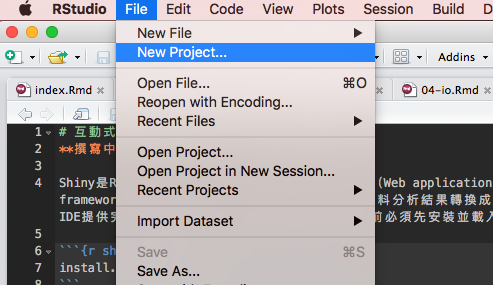
\includegraphics[width=6.85in]{figure/shiny1}

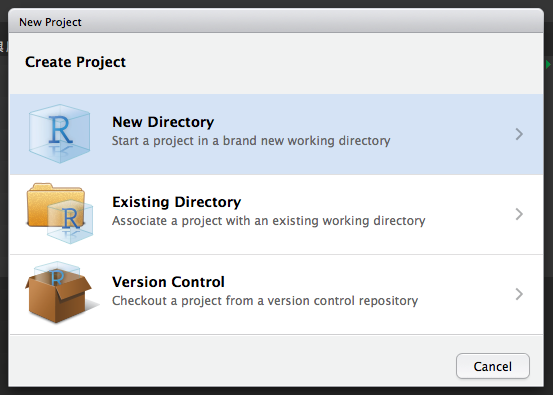
\includegraphics[width=7.68in]{figure/shiny2}

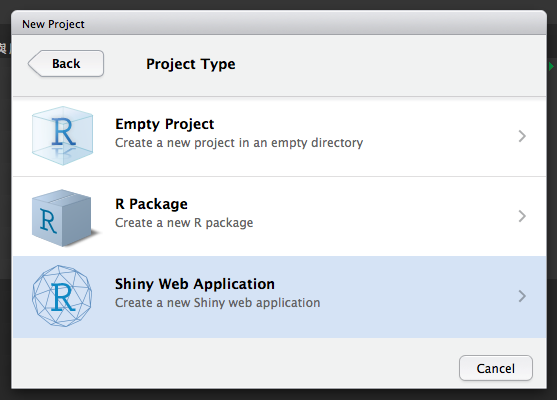
\includegraphics[width=7.74in]{figure/shiny3}

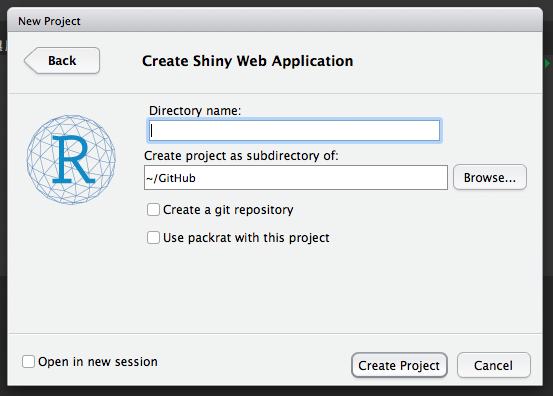
\includegraphics[width=7.68in]{figure/shiny4}

Shiny應用程式包括兩個元件:

\begin{itemize}
\tightlist
\item
  \textbf{ui.R} : 使用者介面(前端)程式碼 user-interface script
\item
  \textbf{server.R} : 伺服器端(後端)程式碼 server script
\end{itemize}

使用者介面程式碼\textbf{ui.R}控制Shiny應用程式的外觀,伺服器端程式碼\textbf{server.R}控制Shiny應用程式的功能。

\textbf{ui.R範例}

\begin{Shaded}
\begin{Highlighting}[]
\KeywordTok{library}\NormalTok{(shiny)}

\KeywordTok{shinyUI}\NormalTok{(}\KeywordTok{fluidPage}\NormalTok{(}

  \CommentTok{# 網頁標題}
  \KeywordTok{titlePanel}\NormalTok{(}\StringTok{"Hello Shiny!"}\NormalTok{),}

  \CommentTok{# Sidebar + slider}
  \KeywordTok{sidebarLayout}\NormalTok{(}
    \KeywordTok{sidebarPanel}\NormalTok{(}
      \KeywordTok{sliderInput}\NormalTok{(}\StringTok{"bins"}\NormalTok{,}
                  \StringTok{"Number of bins:"}\NormalTok{,}
                  \DataTypeTok{min =} \DecValTok{1}\NormalTok{,}
                  \DataTypeTok{max =} \DecValTok{50}\NormalTok{,}
                  \DataTypeTok{value =} \DecValTok{30}\NormalTok{)}
    \NormalTok{),}

    \CommentTok{# 圖形呈現}
    \KeywordTok{mainPanel}\NormalTok{(}
      \KeywordTok{plotOutput}\NormalTok{(}\StringTok{"distPlot"}\NormalTok{)}
    \NormalTok{)}
  \NormalTok{)}
\NormalTok{))}
\end{Highlighting}
\end{Shaded}

\textbf{server.R範例}

\begin{Shaded}
\begin{Highlighting}[]
\KeywordTok{library}\NormalTok{(shiny)}

\KeywordTok{shinyServer}\NormalTok{(function(input, output) \{}

 
  \CommentTok{# 將直方圖Histogram存入distPlot變數,在UI端用plotOutput呈現}
  \NormalTok{output$distPlot <-}\StringTok{ }\KeywordTok{renderPlot}\NormalTok{(\{}
    \NormalTok{x  <-}\StringTok{ }\NormalTok{faithful[, }\DecValTok{2}\NormalTok{]  }\CommentTok{# Old Faithful Geyser data}
    \CommentTok{# input$bins是用UI端的Sidebar + slider調整}
    \NormalTok{bins <-}\StringTok{ }\KeywordTok{seq}\NormalTok{(}\KeywordTok{min}\NormalTok{(x), }\KeywordTok{max}\NormalTok{(x), }\DataTypeTok{length.out =} \NormalTok{input$bins +}\StringTok{ }\DecValTok{1}\NormalTok{)}
    \KeywordTok{hist}\NormalTok{(x, }\DataTypeTok{breaks =} \NormalTok{bins, }\DataTypeTok{col =} \StringTok{'darkgray'}\NormalTok{, }\DataTypeTok{border =} \StringTok{'white'}\NormalTok{)}
  \NormalTok{\})}
\NormalTok{\})}
\end{Highlighting}
\end{Shaded}

若想使用介紹過的Plotly與Shiny結合,可參考\href{https://plot.ly/r/shiny-tutorial/}{此教學網頁}

參考資料

\begin{itemize}
\tightlist
\item
  \href{http://shiny.rstudio.com/}{Shiny官網}
\item
  \href{https://www.rstudio.com/wp-content/uploads/2016/01/shiny-cheatsheet.pdf}{Shiny
  cheat sheet}
\end{itemize}

\chapter{資料探勘}\label{datamining}

\textbf{撰寫中}

\section{什麼是資料探勘}

\textbf{資料探勘(Data
mining)}是用人工智慧、機器學習、統計學和資料庫的交叉方法在相對較大型的資料集中發現模式的計算過程。使用資料探勘技術可以建立從\textbf{輸入資料}學習新資訊,變成智慧的\textbf{演算法}或\textbf{資料模式},\textbf{預測事件}或\textbf{協助決策}。所以,當資料太\texttt{少}或\texttt{太髒}的時候,資料探勘的效力會被影響。

資料探勘要派上用場,必須有以下條件:

\begin{itemize}
\tightlist
\item
  有一些模式/模型可\texttt{學}
\item
  很難定義這些模式/模型
\item
  有資料可\texttt{學}這些模式/模型
\end{itemize}

資料探勘可應用在:

\begin{itemize}
\tightlist
\item
  天氣預測
\item
  搜尋建議、購物建議
\item
  股市預測
\item
  臉部辨識、指紋辨識
\item
  垃圾郵件標記
\item
  尿布啤酒
\end{itemize}

資料探勘的步驟

資料探勘的種類 (依資料性質)

\begin{itemize}
\tightlist
\item
  Supervised learning 監督式學習

  \begin{itemize}
  \tightlist
  \item
    Regression 迴歸:真實的'值'(股票、氣溫)

    \begin{itemize}
    \tightlist
    \item
      Linear Regression 線性迴歸
    \item
      Logistic Regression 羅吉斯迴歸、邏輯迴歸
    \end{itemize}
  \item
    Classification 分類:分兩類(P/N, Yes/No, M/F, Sick/Not
    sick)/分多類 (A/B/C/D)

    \begin{itemize}
    \tightlist
    \item
      Support Vector Machines 支持向量機
    \item
      Decision Trees 決策樹
    \item
      Neural Networks 神經網路
    \item
      K-Nearest Neighbor
    \end{itemize}
  \end{itemize}
\item
  Unsupervised learning 非監督式學習

  \begin{itemize}
  \tightlist
  \item
    Clustering 分群

    \begin{itemize}
    \tightlist
    \item
      Hierarchical clustering 階層式分群
    \item
      K-means clustering
    \end{itemize}
  \item
    Association Rules 關聯式規則
  \end{itemize}
\end{itemize}

\chapter{從小數據到大數據分析}\label{big}

\section{R + Hadoop}\label{r-hadoop}

\section{RHadoop安裝測試流程 (Cloudera)}\label{rhadoop-cloudera}

安裝與測試日期2016/05/12

\subsection{系統/軟體版本資訊}

\begin{itemize}
\tightlist
\item
  Cloudera Hadoop Platform: CDH-5.4.5
  \href{http://www.cloudera.com/downloads/cdh/5-4-5.html}{下載}
\item
  R for Linux 3.3.0
  \href{https://cran.rstudio.com/bin/linux/redhat/README}{安裝說明}
\item
  RStudio Server
  \href{https://www.rstudio.com/products/rstudio/download-server/}{下載}
\item
  RHadoop (latest version on May 12, 2016)
  \href{https://github.com/RevolutionAnalytics/RHadoop/wiki/Downloads}{下載}

  \begin{itemize}
  \tightlist
  \item
    ravro-1.0.3
  \item
    plyrmr-0.6.0
  \item
    rmr-3.3.1
  \item
    rhdfs-1.0.8
  \item
    rhbase-1.2.1
  \end{itemize}
\end{itemize}

\subsection{參考資料}\label{-1}

\begin{itemize}
\tightlist
\item
  \href{https://github.com/RevolutionAnalytics/RHadoop/wiki/Installing-RHadoop-on-RHEL}{RHadoop安裝說明文件}
\item
  \href{https://bigdatastudy.hackpad.com/ep/pad/static/IADMBeqF0vV}{RHadoop安裝步驟}
\item
  \href{http://unix.stackexchange.com/questions/271514/setting-persistent-environment-variable-in-centos-7-issue}{Setting
  persistent environment variable in CentOS 7 issue}
\item
  \href{https://community.cloudera.com/t5/CDH-Manual-Installation/How-to-resolve-quot-Permission-denied-quot-errors-in-CDH/ta-p/36141}{How
  to resolve ``Permission denied'' errors in CDH}
\end{itemize}

\subsection{安裝步驟}

\begin{enumerate}
\def\labelenumi{\arabic{enumi}.}
\tightlist
\item
  下載Cloudera CDH QuickStart VM
  \href{http://www.cloudera.com/developers/get-started-with-hadoop-tutorial.html}{Cloudera
  VM}
\item
  安裝R
  \href{https://cran.rstudio.com/bin/linux/redhat/README}{安裝說明}
\item
  安裝RHadoop
  \href{https://bigdatastudy.hackpad.com/ep/pad/static/IADMBeqF0vV}{RHadoop安裝步驟}
\item
  安裝RStudio Server
  \href{https://www.rstudio.com/products/rstudio/download-server/}{說明}
\end{enumerate}

\subsubsection{Cloudera CDH QuickStart
VM}\label{cloudera-cdh-quickstart-vm}

Cloudera CDH QuickStart
VM是由Cloudera提供的虛擬機器,內涵Linux系統與預載多項Hadoop相關服務,適合想了解Hadoop運作的初學者。

下載VM後,用Virtural Box 開啟即可。

\begin{itemize}
\tightlist
\item
  \href{http://www.cloudera.com/developers/get-started-with-hadoop-tutorial.html}{Cloudera
  CDH QuickStart VM下載處}
\item
  \href{https://www.virtualbox.org/}{Virtural Box下載處}
\end{itemize}

以下安裝步驟都在Cloudera CDH QuickStart VM內進行

\subsubsection{安裝R}\label{r}

\begin{itemize}
\tightlist
\item
  Cloudera CDH用的Linux作業系統是CentOS
\item
  依照安裝說明,需要先安裝Extra Packages for Enterprise Linux
  (EPEL),但系統內有預載,所以可以不用按照說明重新下載安裝,直接執行\texttt{sudo\ yum\ install\ epel-release}指令即可
\item
  步驟:安裝最新EPRL,更新yum,安裝R。打開Terminal輸入以下指令。
\end{itemize}

\begin{verbatim}
sudo yum install epel-release
sudo yum update
sudo yum install R
\end{verbatim}

\subsubsection{安裝RHadoop-1 先進行環境設定}\label{rhadoop-1-}

設定\texttt{HADOOP\_CMD}與\texttt{HADOOP\_STREAMING}兩項環境參數,路徑可能會不同(尤其是\texttt{HADOOP\_STREAMING})

\begin{enumerate}
\def\labelenumi{\arabic{enumi}.}
\item
  尋找\texttt{HADOOP\_STREAMING}路徑方法

\begin{verbatim}
find / -name hadoop-streaming-*.jar
\end{verbatim}
\item
  設定\texttt{HADOOP\_CMD}與\texttt{HADOOP\_STREAMING}兩項環境參數,路徑記得換成自己的

\begin{verbatim}
echo export HADOOP_CMD="/usr/bin/hadoop">/etc/profile.d/hadoopenv.sh
echo export HADOOP_STREAMING=
"/opt/cloudera/parcels/CDH-5.4.5-1.cdh5.4.5.p0.7/lib/hadoop-mapreduce/
    hadoop-streaming-2.6.0-cdh5.4.5.jar" > /etc/profile.d/hadoopenv.sh
chmod 0755 /etc/profile.d/hadoopenv.sh
\end{verbatim}
\end{enumerate}

\subsubsection{安裝RHadoop-2 rmr2}\label{rhadoop-2-rmr2}

\begin{itemize}
\tightlist
\item
  每個Node都要裝
\item
  安裝前先至\href{https://github.com/RevolutionAnalytics/rmr2/blob/master/pkg/DESCRIPTION}{說明檔}看需要先安裝哪些其他的packages,Depends
  和 Imports 所列的packages都要裝
\item
  以下為安裝packages的程式碼,在R內執行(在Terminal輸入\texttt{R},就能進入R軟體)
\end{itemize}

\begin{Shaded}
\begin{Highlighting}[]
\KeywordTok{install.packages}\NormalTok{(}\KeywordTok{c}\NormalTok{(}\StringTok{"methods"}\NormalTok{,}\StringTok{"Rcpp"}\NormalTok{, }\StringTok{"RJSONIO"}\NormalTok{, }\StringTok{"digest"}\NormalTok{, }\StringTok{"functional"}\NormalTok{, }
                   \StringTok{"reshape2"}\NormalTok{,}\StringTok{"stringr"}\NormalTok{, }\StringTok{"plyr"}\NormalTok{, }\StringTok{"caTools"}\NormalTok{,}\StringTok{"quickcheck"}\NormalTok{,}\StringTok{"testthat"}\NormalTok{), }
                 \DataTypeTok{dependencies=}\OtherTok{TRUE}\NormalTok{, }\DataTypeTok{repos=}\StringTok{'http://cran.rstudio.com/'}\NormalTok{)}
\end{Highlighting}
\end{Shaded}

\begin{itemize}
\tightlist
\item
  使用\texttt{q()}指令,跳出R軟體
\item
  \href{https://github.com/RevolutionAnalytics/RHadoop/wiki/Downloads}{下載rmr2}
\item
  安裝(請將\texttt{rmr2\_2.3.0.tar.gz}替換成剛剛下載的安裝檔路徑)
\end{itemize}

\begin{verbatim}
sudo R CMD INSTALL rmr2_2.3.0.tar.gz
\end{verbatim}

\subsubsection{安裝RHadoop-3 rhdfs}\label{rhadoop-3-rhdfs}

\begin{itemize}
\tightlist
\item
  只要裝在會跑R的那個Node
\item
  在裝之前,先Check是否有安裝JDK (測試JDK 1.8.0\_91沒問題)
\item
  Check環境變數JAVA\_HOME是否有設好
\end{itemize}

\begin{verbatim}
echo $JAVA_HOME
\end{verbatim}

若什麼都沒有回傳,先設定環境變數(將\texttt{/usr/java/jdk1.8.0\_91}換成自己的路徑)

\begin{verbatim}
echo export JAVA_HOME="/usr/java/jdk1.8.0_91">/etc/profile.d/jdkenv.sh
\end{verbatim}

為了讓R可以跑JAVA,在Terminal輸入

\begin{verbatim}
R CMD javareconf
\end{verbatim}

然後進到R程式(在Terminal輸入\texttt{R},就能進入R軟體),安裝\texttt{rJava}
package

\begin{Shaded}
\begin{Highlighting}[]
\KeywordTok{install.packages}\NormalTok{(}\StringTok{"rJava"}\NormalTok{,}\DataTypeTok{dependencies=}\OtherTok{TRUE}\NormalTok{, }\DataTypeTok{repos=}\StringTok{'http://cran.rstudio.com/'}\NormalTok{)\{target=}\StringTok{"_blank"}\NormalTok{\}}
\end{Highlighting}
\end{Shaded}

最後跳出R程式,\href{https://github.com/RevolutionAnalytics/RHadoop/wiki/Downloads}{下載rhdfs},安裝rhdfs

\begin{itemize}
\tightlist
\item
  將\texttt{/usr/bin/hadoop}換成自己的\texttt{HADOOP\_CMD}路徑
\item
  \texttt{rhdfs\_1.0.8.tar.gz}換成下載的安裝檔路徑)
\end{itemize}

\begin{verbatim}
sudo HADOOP_CMD=/usr/bin/hadoop R CMD INSTALL rhdfs_1.0.8.tar.gz
\end{verbatim}

\subsection{測試前,先解決權限問題}

\begin{itemize}
\tightlist
\item
  預設hdfs的存取權限不足,所以要打開
\item
  將\texttt{user01}改為自己的使用者名稱
\end{itemize}

\begin{verbatim}
sudo -u hdfs hadoop fs -mkdir /user/user01
sudo -u hdfs hadoop fs -chown user01 /user/user01
\end{verbatim}

\subsection{測試}

進入R測試以下程式碼是否能執行

\begin{Shaded}
\begin{Highlighting}[]
\KeywordTok{Sys.setenv}\NormalTok{(}\DataTypeTok{HADOOP_CMD=}\StringTok{"/usr/bin/hadoop"}\NormalTok{)}
\KeywordTok{Sys.setenv}\NormalTok{(}\DataTypeTok{HADOOP_STREAMING=}\StringTok{"/opt/cloudera/parcels/CDH-5.4.5-1.cdh5.4.5.p0.7/lib/hadoop-mapreduce/hadoop-streaming-2.6.0-cdh5.4.5.jar"}\NormalTok{)}
\KeywordTok{library}\NormalTok{(rmr2)}
\CommentTok{#test mapreduce}
\NormalTok{small.ints =}\StringTok{ }\KeywordTok{to.dfs}\NormalTok{(}\DecValTok{1}\NormalTok{:}\DecValTok{100}\NormalTok{)}
\NormalTok{out<-}\KeywordTok{mapreduce}\NormalTok{(}
    \DataTypeTok{input =} \NormalTok{small.ints, }
    \DataTypeTok{map =} \NormalTok{function(., v) }\KeywordTok{cbind}\NormalTok{(v, v^}\DecValTok{2}\NormalTok{))}
\KeywordTok{head}\NormalTok{(}\KeywordTok{from.dfs}\NormalTok{(out))}
\end{Highlighting}
\end{Shaded}

\subsection{安裝RStudio Server}\label{rstudio-server}

\href{https://www.rstudio.com/products/rstudio/download-server/}{官方下載與安裝說明}

在Terminal執行以下程式碼

\begin{itemize}
\tightlist
\item
  檔案連結\texttt{https://download2.rstudio.org/rstudio-server-rhel-0.99.896-x86\_64.rpm}可能有最新版,請Check\href{https://www.rstudio.com/products/rstudio/download-server/}{官網}
\end{itemize}

\begin{verbatim}
wget https://download2.rstudio.org/rstudio-server-rhel-0.99.896-x86_64.rpm
sudo yum install --nogpgcheck rstudio-server-rhel-0.99.896-x86_64.rpm
\end{verbatim}

打開瀏覽器,輸入\texttt{http://localhost:8787/},就能進入RStudio
Server了!

測完收工~

\section{RHadoop MapReduce: easy word
count}\label{rhadoop-mapreduce-easy-word-count}

\begin{Shaded}
\begin{Highlighting}[]
\NormalTok{Debate<-}\KeywordTok{readLines}\NormalTok{(}\StringTok{"https://raw.githubusercontent.com/CGUIM-BigDataAnalysis/BigDataCGUIM/master/104/RepDebateMiami.txt"}\NormalTok{)}
\NormalTok{DebateSplit<-}\KeywordTok{unlist}\NormalTok{(}\KeywordTok{strsplit}\NormalTok{(}\KeywordTok{tolower}\NormalTok{(Debate),}\DataTypeTok{split =} \StringTok{' |}\CharTok{\textbackslash{}\textbackslash{}}\StringTok{.|}\CharTok{\textbackslash{}\textbackslash{}}\StringTok{,|}\CharTok{\textbackslash{}\textbackslash{}}\StringTok{?'}\NormalTok{))}
\CommentTok{#table(DebateSplit)}
\end{Highlighting}
\end{Shaded}

\begin{Shaded}
\begin{Highlighting}[]
\NormalTok{DebateSplitDFS =}\StringTok{ }\KeywordTok{to.dfs}\NormalTok{(DebateSplit)}
\NormalTok{result =}\StringTok{ }\KeywordTok{mapreduce}\NormalTok{(}
    \DataTypeTok{input =} \NormalTok{DebateSplitDFS,}
    \DataTypeTok{map =} \NormalTok{function(.,v) }\KeywordTok{keyval}\NormalTok{(v, }\DecValTok{1}\NormalTok{),}
    \DataTypeTok{reduce =} \NormalTok{function(k,vv) }\KeywordTok{keyval}\NormalTok{(k, }\KeywordTok{sum}\NormalTok{(vv)))}
\KeywordTok{head}\NormalTok{(result)}
\end{Highlighting}
\end{Shaded}

\section{R + Spark}\label{r-spark}

sparklyr SparkR

Supports dplyr, Spark ML and H2O Distributed on CRAN Easy to install
Extensible

測試環境

\begin{itemize}
\tightlist
\item
  R version 3.3.2 (2016-10-31)
\item
  Platform: x86\_64-w64-mingw32/x64 (64-bit)
\item
  Running under: Windows \textgreater{}= 8 x64 (build 9200)
\item
  sparklyr\_0.5.3-9002
\end{itemize}

\begin{Shaded}
\begin{Highlighting}[]
\KeywordTok{install.packages}\NormalTok{(}\StringTok{"sparklyr"}\NormalTok{)}
\CommentTok{#devtools::install_github("rstudio/sparklyr")}
\end{Highlighting}
\end{Shaded}

\begin{Shaded}
\begin{Highlighting}[]
\KeywordTok{library}\NormalTok{(sparklyr)}
\KeywordTok{spark_install}\NormalTok{(}\DataTypeTok{version =} \StringTok{"2.1.0"}\NormalTok{)}
\end{Highlighting}
\end{Shaded}

\begin{Shaded}
\begin{Highlighting}[]
\CommentTok{#Sys.setenv(SPARK_HOME="C:/Users/yjtseng/AppData/Local/rstudio/spark/Cache/spark-2.0.1-bin-hadoop2.7")}
\CommentTok{#Sys.setenv(HADOOP_HOME="C:\textbackslash{}\textbackslash{}Program Files\textbackslash{}\textbackslash{}RStudio\textbackslash{}\textbackslash{}bin\textbackslash{}\textbackslash{}winutils\textbackslash{}\textbackslash{}x64\textbackslash{}\textbackslash{}")}
\KeywordTok{library}\NormalTok{(sparklyr)}
\KeywordTok{library}\NormalTok{(dplyr)}
\NormalTok{sc <-}\StringTok{ }\KeywordTok{spark_connect}\NormalTok{(}\DataTypeTok{master =} \StringTok{"local"}\NormalTok{, }\DataTypeTok{version =} \StringTok{"2.1.0"}\NormalTok{)}
\end{Highlighting}
\end{Shaded}

\begin{Shaded}
\begin{Highlighting}[]
\KeywordTok{install.packages}\NormalTok{(}\KeywordTok{c}\NormalTok{(}\StringTok{"nycflights13"}\NormalTok{, }\StringTok{"Lahman"}\NormalTok{))}
\end{Highlighting}
\end{Shaded}

\begin{Shaded}
\begin{Highlighting}[]
\NormalTok{iris_tbl <-}\StringTok{ }\KeywordTok{copy_to}\NormalTok{(sc, iris)}
\NormalTok{flights_tbl <-}\StringTok{ }\KeywordTok{copy_to}\NormalTok{(sc, nycflights13::flights, }\StringTok{"flights"}\NormalTok{)}
\NormalTok{batting_tbl <-}\StringTok{ }\KeywordTok{copy_to}\NormalTok{(sc, Lahman::Batting, }\StringTok{"batting"}\NormalTok{)}
\KeywordTok{src_tbls}\NormalTok{(sc)}
\NormalTok{flights_tbl %>%}\StringTok{ }\KeywordTok{filter}\NormalTok{(dep_delay ==}\StringTok{ }\DecValTok{2}\NormalTok{)}
\end{Highlighting}
\end{Shaded}

\begin{verbatim}
Source:   query [6,233 x 19]
Database: spark connection master=local[8] app=sparklyr local=TRUE

    year month   day dep_time sched_dep_time dep_delay arr_time sched_arr_time arr_delay
   <int> <int> <int>    <int>          <int>     <dbl>    <int>          <int>     <dbl>
1   2013     1     1      517            515         2      830            819        11
2   2013     1     1      542            540         2      923            850        33
3   2013     1     1      702            700         2     1058           1014        44
4   2013     1     1      715            713         2      911            850        21
5   2013     1     1      752            750         2     1025           1029        -4
6   2013     1     1      917            915         2     1206           1211        -5
7   2013     1     1      932            930         2     1219           1225        -6
8   2013     1     1     1028           1026         2     1350           1339        11
9   2013     1     1     1042           1040         2     1325           1326        -1
10  2013     1     1     1231           1229         2     1523           1529        -6
# ... with 6,223 more rows, and 10 more variables: carrier <chr>, flight <int>,
#   tailnum <chr>, origin <chr>, dest <chr>, air_time <dbl>, distance <dbl>, hour <dbl>,
#   minute <dbl>, time_hour <dbl>
\end{verbatim}

\begin{Shaded}
\begin{Highlighting}[]
\KeywordTok{spark_disconnect}\NormalTok{(sc)}
\end{Highlighting}
\end{Shaded}

在RStudio中有整合Spark連線功能,右上角的Spark頁籤可供使用者開啟特定版本的Spark
connections,除此之外,也可使用Spark頁籤瀏覽在Spark中的表格結構與資料的前1000列。

參考資料

\begin{itemize}
\tightlist
\item
  \url{http://spark.rstudio.com/}
\item
  \url{https://shiring.github.io/machine_learning/2017/02/19/food_spark}
\end{itemize}

\chapter{軟體安裝介紹}\label{install}

本章節將介紹R與RStudio的安裝與基本使用方式

\section{R安裝}\label{r}

\href{http://www.r-project.org/}{R語言}是一種自由軟體程式語言,主要用於資料分析與統計運算,2000年時終於發表R
1.0.0,有關R語言的發展歷史可參考\href{https://zh.wikipedia.org/wiki/R\%E8\%AF\%AD\%E8\%A8\%80}{維基百科}。

安裝步驟如下:

\textbf{Step 1. 從R的官網下載安裝檔}

\begin{itemize}
\tightlist
\item
  進入R官網 \url{https://www.r-project.org/}
\item
  選擇\textbf{Download}下方的\textbf{CRAN}連結
\item
  進入CRAN子網頁後,請選擇離所在地最近的載點,以臺灣桃園為例,可選擇元智大學
  ( Department of Computer Science and Engineering, Yuan Ze University)
  的載點。
\end{itemize}

進入下載網頁後,可看到多個選項:

\begin{itemize}
\tightlist
\item
  Download R for Linux
\item
  Download R for (Mac) OS X
\item
  Download R for Windows
\end{itemize}

依作業系統選擇適當連結後,點選\textbf{base} (Binaries for base
distribution),下載最新版本的R安裝檔。

\textbf{Step 2. 依安裝檔指示完成安裝}

\section{RStudio安裝}\label{rstudio}

\href{https://www.rstudio.com/}{RStudio}是R語言的IDE,屬於免費自由軟體,提供一般桌面板與伺服器版,以下介紹桌面板安裝方式,伺服器版安裝可參考Chapter
\ref{big}。

\textbf{Step 1. 從RStudio的官網下載安裝檔}

\begin{itemize}
\tightlist
\item
  進入RStudio官網 \url{https://www.rstudio.com/}
\item
  選擇網頁上方\textbf{Products}連結內的\textbf{RStudio}
\item
  選擇\textbf{Desktop}版本
\item
  點選\textbf{Open Source Edition}下方的\textbf{DOWNLOAD RSTUDIO
  DESKTOP}
\item
  點選RStudio Desktop Open Source License下方的\textbf{DOWNLOAD}
\end{itemize}

選單中會出現多種作業系統版本,以RStudio 1.0.136為例,各作業系統版本如下

\begin{itemize}
\tightlist
\item
  RStudio 1.0.136 - Windows Vista/7/8/10\\
\item
  RStudio 1.0.136 - Mac OS X 10.6+ (64-bit)
\item
  RStudio 1.0.136 - Ubuntu 12.04+/Debian 8+ (32-bit)
\item
  RStudio 1.0.136 - Ubuntu 12.04+/Debian 8+ (64-bit)
\item
  RStudio 1.0.136 - Fedora 19+/RedHat 7+/openSUSE 13.1+ (32-bit)
\item
  RStudio 1.0.136 - Fedora 19+/RedHat 7+/openSUSE 13.1+ (64-bit)
\end{itemize}

依作業系統選擇適當連結

\textbf{Step 2. 依安裝檔指示完成安裝}

\section{RStudio使用簡介}\label{rstudio}

\subsection{專案}

RStudio引進專案(Project)的概念,幫助使用者管理同一專案之R程式碼檔案,同時完成工作路徑的設定
(設定為專案所在資料夾)。除快速測試外,建議一開始就以專案形式新增R程式碼。

以本課程為例,開啟RStudio視窗後,可在左上\textbf{File}選項中選擇\textbf{New
Project}後,依需求選擇\textbf{New Directory}或\textbf{Existing
Directory}

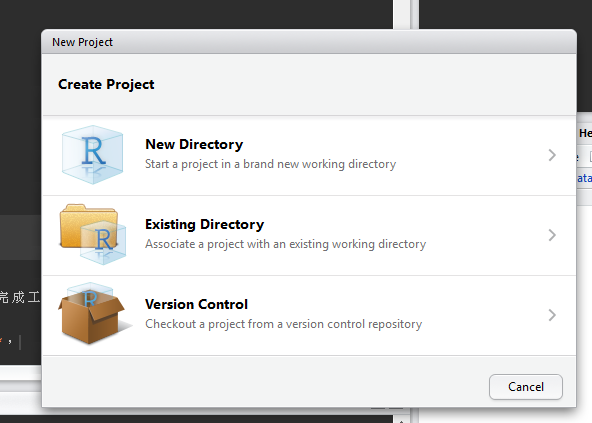
\includegraphics[width=8.22in]{figure/NewProject}

若選擇的是\textbf{New Directory},則會出現下列三個選項

\begin{itemize}
\tightlist
\item
  Empty Project
\item
  R Package
\item
  Shiny Web Application
\end{itemize}

若是新增一般分析專案,選擇\textbf{Empty
Project}後,輸入\textbf{專案路徑}與\textbf{專案名稱},完成專案新增。

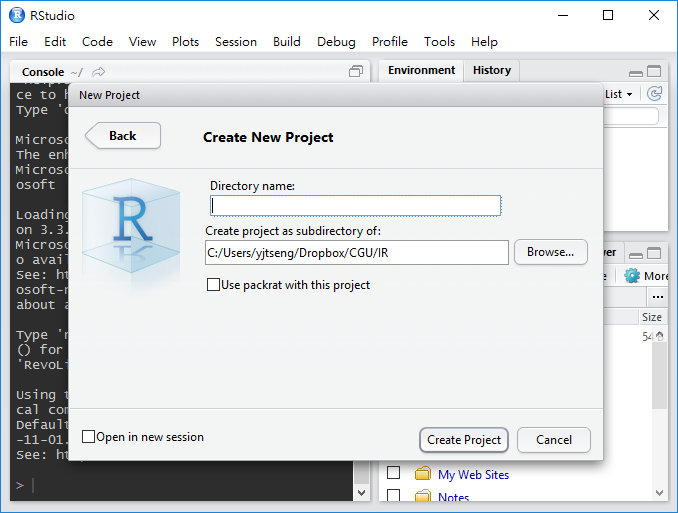
\includegraphics[width=9.42in]{figure/NewProject1}

完成專案新增後,在專案內新增R程式碼檔案(File -\textgreater{} New file
-\textgreater{} R Script)後,\textbf{程式碼編輯區 Source
editor}就會出現在左上角。

\subsection{RStudio介面}\label{rstudio}

RStudio的介面共有四個區塊,分別為

\begin{itemize}
\tightlist
\item
  程式碼編輯區 Source editor
\item
  執行視窗 Console
\item
  環境/物件
\item
  檔案/圖表/說明文件
\end{itemize}

剛開啟一個新的RStudio視窗時不會有\textbf{程式碼編輯區 Source
editor},必須要新增專案後才會出現。

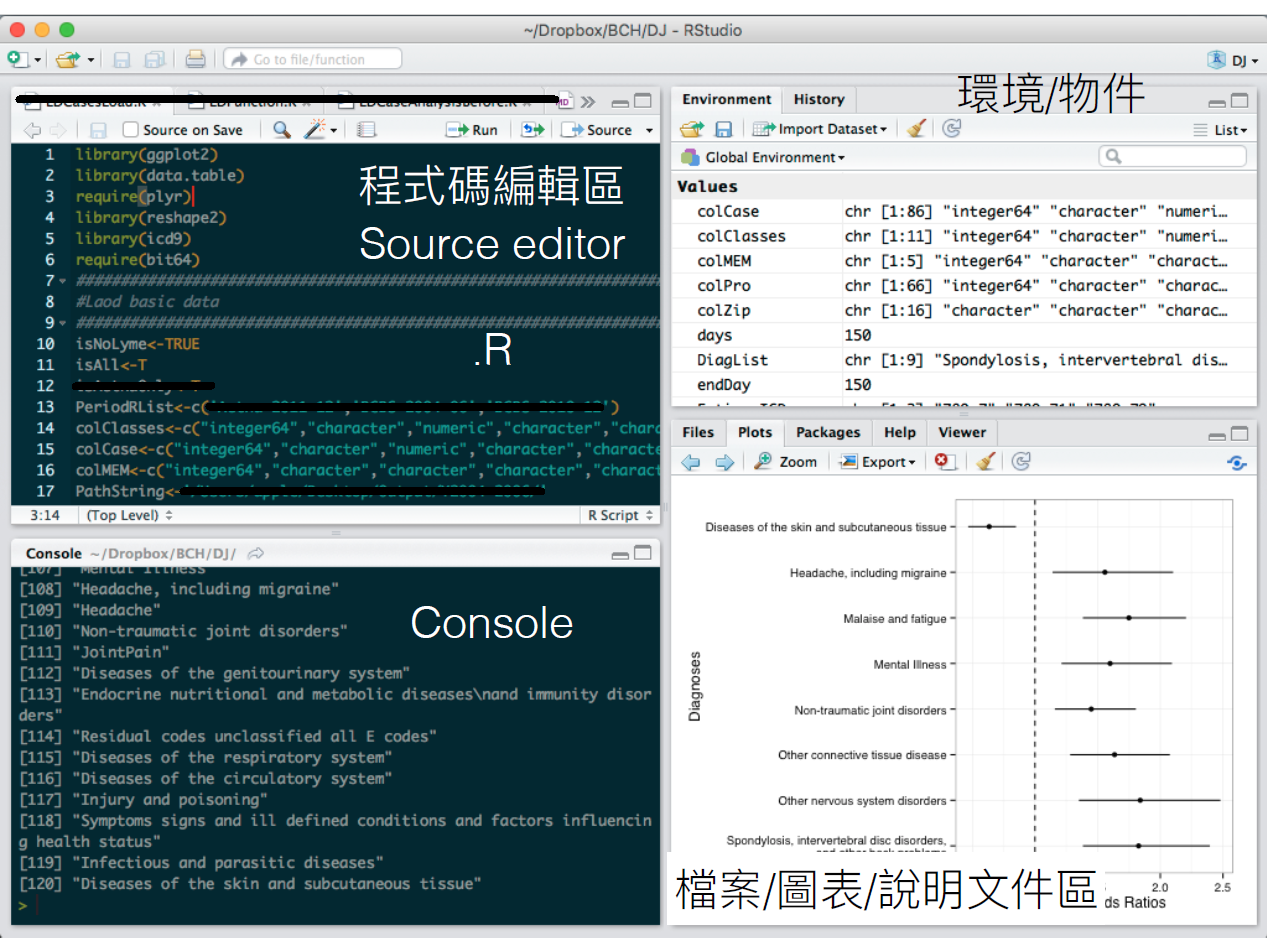
\includegraphics[width=17.6in]{figure/RStudio}

建議使用方式如下:

\begin{itemize}
\tightlist
\item
  在左上方\textbf{程式碼編輯區 Source editor}撰寫程式碼
\item
  完成程式碼撰寫後,將需要執行的程式碼反白,點選\textbf{Run}
  (見下圖),執行程式碼
\item
  除了反白外,將游標移至需要執行的程式碼,,點選\textbf{Run}
  (見下圖)也可執行該行程式碼
\item
  程式碼會在左下方Console視窗執行,顯示結果
\item
  如果有畫圖,會出現在右下方視窗
\item
  可在右上方視窗檢查所有變數
\end{itemize}

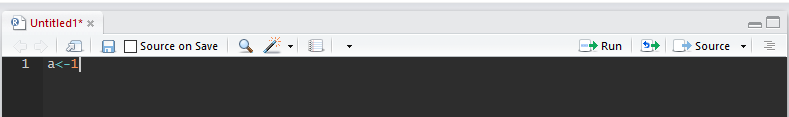
\includegraphics[width=10.96in]{figure/ed}

RStudio的其他使用細節,可參考\href{https://www.rstudio.com/wp-content/uploads/2016/01/rstudio-IDE-cheatsheet.pdf}{RStudio
IDE Cheat Sheet}

\chapter*{作者資訊}\label{author}
\addcontentsline{toc}{chapter}{作者資訊}

曾意儒 Yi-Ju Tseng

\href{http://im.cgu.edu.tw/bin/home.php}{長庚大學 資訊管理學系} 助理教授

\href{http://yijutseng.github.io}{個人網站}

Lab: \href{https://dhlab-cgu.github.io/}{數位健康實驗室}

歡迎提供\href{https://goo.gl/forms/5Htobvwy2vsB7yiF3}{建議與回饋}

\bibliography{packages.bib,book.bib}


\end{document}
